\documentclass[twoside]{book}

% Packages required by doxygen
\usepackage{fixltx2e}
\usepackage{calc}
\usepackage{doxygen}
\usepackage[export]{adjustbox} % also loads graphicx
\usepackage{graphicx}
\usepackage[utf8]{inputenc}
\usepackage{makeidx}
\usepackage{multicol}
\usepackage{multirow}
\PassOptionsToPackage{warn}{textcomp}
\usepackage{textcomp}
\usepackage[nointegrals]{wasysym}
\usepackage[table]{xcolor}

% Font selection
\usepackage[T1]{fontenc}
\usepackage[scaled=.90]{helvet}
\usepackage{courier}
\usepackage{amssymb}
\usepackage{sectsty}
\renewcommand{\familydefault}{\sfdefault}
\allsectionsfont{%
  \fontseries{bc}\selectfont%
  \color{darkgray}%
}
\renewcommand{\DoxyLabelFont}{%
  \fontseries{bc}\selectfont%
  \color{darkgray}%
}
\newcommand{\+}{\discretionary{\mbox{\scriptsize$\hookleftarrow$}}{}{}}

% Page & text layout
\usepackage{geometry}
\geometry{%
  a4paper,%
  top=2.5cm,%
  bottom=2.5cm,%
  left=2.5cm,%
  right=2.5cm%
}
\tolerance=750
\hfuzz=15pt
\hbadness=750
\setlength{\emergencystretch}{15pt}
\setlength{\parindent}{0cm}
\setlength{\parskip}{3ex plus 2ex minus 2ex}
\makeatletter
\renewcommand{\paragraph}{%
  \@startsection{paragraph}{4}{0ex}{-1.0ex}{1.0ex}{%
    \normalfont\normalsize\bfseries\SS@parafont%
  }%
}
\renewcommand{\subparagraph}{%
  \@startsection{subparagraph}{5}{0ex}{-1.0ex}{1.0ex}{%
    \normalfont\normalsize\bfseries\SS@subparafont%
  }%
}
\makeatother

% Headers & footers
\usepackage{fancyhdr}
\pagestyle{fancyplain}
\fancyhead[LE]{\fancyplain{}{\bfseries\thepage}}
\fancyhead[CE]{\fancyplain{}{}}
\fancyhead[RE]{\fancyplain{}{\bfseries\leftmark}}
\fancyhead[LO]{\fancyplain{}{\bfseries\rightmark}}
\fancyhead[CO]{\fancyplain{}{}}
\fancyhead[RO]{\fancyplain{}{\bfseries\thepage}}
\fancyfoot[LE]{\fancyplain{}{}}
\fancyfoot[CE]{\fancyplain{}{}}
\fancyfoot[RE]{\fancyplain{}{\bfseries\scriptsize Generated by Doxygen }}
\fancyfoot[LO]{\fancyplain{}{\bfseries\scriptsize Generated by Doxygen }}
\fancyfoot[CO]{\fancyplain{}{}}
\fancyfoot[RO]{\fancyplain{}{}}
\renewcommand{\footrulewidth}{0.4pt}
\renewcommand{\chaptermark}[1]{%
  \markboth{#1}{}%
}
\renewcommand{\sectionmark}[1]{%
  \markright{\thesection\ #1}%
}

% Indices & bibliography
\usepackage{natbib}
\usepackage[titles]{tocloft}
\setcounter{tocdepth}{3}
\setcounter{secnumdepth}{5}
\makeindex

% Hyperlinks (required, but should be loaded last)
\usepackage{ifpdf}
\ifpdf
  \usepackage[pdftex,pagebackref=true]{hyperref}
\else
  \usepackage[ps2pdf,pagebackref=true]{hyperref}
\fi
\hypersetup{%
  colorlinks=true,%
  linkcolor=blue,%
  citecolor=blue,%
  unicode%
}

% Custom commands
\newcommand{\clearemptydoublepage}{%
  \newpage{\pagestyle{empty}\cleardoublepage}%
}

\usepackage{caption}
\captionsetup{labelsep=space,justification=centering,font={bf},singlelinecheck=off,skip=4pt,position=top}

%===== C O N T E N T S =====

\begin{document}

% Titlepage & ToC
\hypersetup{pageanchor=false,
             bookmarksnumbered=true,
             pdfencoding=unicode
            }
\pagenumbering{alph}
\begin{titlepage}
\vspace*{7cm}
\begin{center}%
{\Large Mturk \\[1ex]\large 1.\+0.\+0 }\\
\vspace*{1cm}
{\large Generated by Doxygen 1.8.14}\\
\end{center}
\end{titlepage}
\clearemptydoublepage
\pagenumbering{roman}
\tableofcontents
\clearemptydoublepage
\pagenumbering{arabic}
\hypersetup{pageanchor=true}

%--- Begin generated contents ---
\chapter{Namespace Index}
\section{Packages}
Here are the packages with brief descriptions (if available)\+:\begin{DoxyCompactList}
\item\contentsline{section}{\mbox{\hyperlink{namespace_utility_system}{Utility\+System}} }{\pageref{namespace_utility_system}}{}
\end{DoxyCompactList}

\chapter{Hierarchical Index}
\section{Class Hierarchy}
This inheritance list is sorted roughly, but not completely, alphabetically\+:\begin{DoxyCompactList}
\item \contentsline{section}{Base\+Connection$<$ Node $>$}{\pageref{class_base_connection}}{}
\begin{DoxyCompactList}
\item \contentsline{section}{Node\+Edge}{\pageref{class_node_edge}}{}
\end{DoxyCompactList}
\item \contentsline{section}{Circum\+Circ}{\pageref{struct_circum_circ}}{}
\item \contentsline{section}{Utility\+System.\+Decision\+Context}{\pageref{class_utility_system_1_1_decision_context}}{}
\item \contentsline{section}{Delaunay\+Triangle}{\pageref{struct_delaunay_triangle}}{}
\item \contentsline{section}{Simplex\+Noise.\+Grad}{\pageref{class_simplex_noise_1_1_grad}}{}
\item \contentsline{section}{Grid2D}{\pageref{struct_grid2_d}}{}
\item \contentsline{section}{Grid\+Factory}{\pageref{class_grid_factory}}{}
\item \contentsline{section}{Heuristic$<$ Int\+Point $>$}{\pageref{class_heuristic}}{}
\begin{DoxyCompactList}
\item \contentsline{section}{Euclidean\+Heuristic}{\pageref{class_euclidean_heuristic}}{}
\end{DoxyCompactList}
\item I\+Comparable\begin{DoxyCompactList}
\item \contentsline{section}{Utility\+System.\+Decision}{\pageref{class_utility_system_1_1_decision}}{}
\begin{DoxyCompactList}
\item \contentsline{section}{Spawn\+Decision}{\pageref{class_spawn_decision}}{}
\end{DoxyCompactList}
\item \contentsline{section}{Utility\+System.\+Utility\+Properties}{\pageref{class_utility_system_1_1_utility_properties}}{}
\end{DoxyCompactList}
\item \contentsline{section}{I\+Connection$<$ T $>$}{\pageref{interface_i_connection}}{}
\begin{DoxyCompactList}
\item \contentsline{section}{Base\+Connection$<$ T $>$}{\pageref{class_base_connection}}{}
\end{DoxyCompactList}
\item \contentsline{section}{I\+Connection$<$ Int\+Point $>$}{\pageref{interface_i_connection}}{}
\item \contentsline{section}{I\+Graph$<$ T $>$}{\pageref{interface_i_graph}}{}
\item \contentsline{section}{I\+Graph$<$ Int\+Point $>$}{\pageref{interface_i_graph}}{}
\begin{DoxyCompactList}
\item \contentsline{section}{Tile\+Graph}{\pageref{class_tile_graph}}{}
\end{DoxyCompactList}
\item \contentsline{section}{I\+Has\+Connections$<$ T $>$}{\pageref{interface_i_has_connections}}{}
\item \contentsline{section}{I\+Has\+Connections$<$ Node $>$}{\pageref{interface_i_has_connections}}{}
\begin{DoxyCompactList}
\item \contentsline{section}{Node}{\pageref{class_node}}{}
\begin{DoxyCompactList}
\item \contentsline{section}{Grid\+Face}{\pageref{class_grid_face}}{}
\end{DoxyCompactList}
\end{DoxyCompactList}
\item \contentsline{section}{Int\+Point}{\pageref{struct_int_point}}{}
\item \contentsline{section}{Int\+Triangle}{\pageref{struct_int_triangle}}{}
\item \contentsline{section}{Math\+Ops}{\pageref{class_math_ops}}{}
\item \contentsline{section}{Mesh\+Data}{\pageref{class_mesh_data}}{}
\item Mono\+Behaviour\begin{DoxyCompactList}
\item \contentsline{section}{Clutter\+Placement}{\pageref{class_clutter_placement}}{}
\item \contentsline{section}{Delaunay\+Triangulation}{\pageref{class_delaunay_triangulation}}{}
\item \contentsline{section}{Game\+Node}{\pageref{class_game_node}}{}
\item \contentsline{section}{Generation\+Algorithm}{\pageref{class_generation_algorithm}}{}
\begin{DoxyCompactList}
\item \contentsline{section}{Biome\+Generator}{\pageref{class_biome_generator}}{}
\item \contentsline{section}{City\+Generator}{\pageref{class_city_generator}}{}
\item \contentsline{section}{Generation\+Sequence}{\pageref{class_generation_sequence}}{}
\item \contentsline{section}{Noise\+Generator}{\pageref{class_noise_generator}}{}
\begin{DoxyCompactList}
\item \contentsline{section}{Perlin\+Octaves}{\pageref{class_perlin_octaves}}{}
\item \contentsline{section}{Simplex\+Noise}{\pageref{class_simplex_noise}}{}
\end{DoxyCompactList}
\item \contentsline{section}{Terrain\+Generator}{\pageref{class_terrain_generator}}{}
\end{DoxyCompactList}
\item \contentsline{section}{Generation\+Controller}{\pageref{class_generation_controller}}{}
\item \contentsline{section}{Graph\+Builder}{\pageref{class_graph_builder}}{}
\item \contentsline{section}{Heuristic$<$ T $>$}{\pageref{class_heuristic}}{}
\item \contentsline{section}{Map\+Display}{\pageref{class_map_display}}{}
\item \contentsline{section}{Map\+Generator}{\pageref{class_map_generator}}{}
\item \contentsline{section}{Noise\+Map}{\pageref{class_noise_map}}{}
\item \contentsline{section}{Object\+Picker}{\pageref{class_object_picker}}{}
\item \contentsline{section}{Path\+Following}{\pageref{class_path_following}}{}
\item \contentsline{section}{Path\+Smoother}{\pageref{class_path_smoother}}{}
\item \contentsline{section}{Point\+Generator}{\pageref{class_point_generator}}{}
\begin{DoxyCompactList}
\item \contentsline{section}{Poisson\+Disk\+Sampling}{\pageref{class_poisson_disk_sampling}}{}
\end{DoxyCompactList}
\item \contentsline{section}{Poly\+Grid}{\pageref{class_poly_grid}}{}
\item \contentsline{section}{Simplex\+Terrain\+Generator}{\pageref{class_simplex_terrain_generator}}{}
\item \contentsline{section}{Tile\+A\+Star}{\pageref{class_tile_a_star}}{}
\item \contentsline{section}{Tile\+Graph}{\pageref{class_tile_graph}}{}
\item \contentsline{section}{Tile\+World}{\pageref{class_tile_world}}{}
\item \contentsline{section}{Utility\+System.\+Consideration}{\pageref{class_utility_system_1_1_consideration}}{}
\item \contentsline{section}{Utility\+System.\+Decision}{\pageref{class_utility_system_1_1_decision}}{}
\item \contentsline{section}{Utility\+System.\+Decision\+Maker}{\pageref{class_utility_system_1_1_decision_maker}}{}
\item \contentsline{section}{Utility\+System.\+Decision\+Score\+Evaluator}{\pageref{class_utility_system_1_1_decision_score_evaluator}}{}
\item \contentsline{section}{Utility\+System.\+Utility\+Properties}{\pageref{class_utility_system_1_1_utility_properties}}{}
\item \contentsline{section}{World\+Gen\+Context}{\pageref{class_world_gen_context}}{}
\end{DoxyCompactList}
\item \contentsline{section}{Noise\+Data}{\pageref{struct_noise_data}}{}
\item \contentsline{section}{Random\+Queue$<$ T $>$}{\pageref{class_random_queue}}{}
\item \contentsline{section}{Random\+Queue$<$ Vector2 $>$}{\pageref{class_random_queue}}{}
\item \contentsline{section}{Square\+Grid\+Params}{\pageref{struct_square_grid_params}}{}
\item \contentsline{section}{Terrain\+Type}{\pageref{struct_terrain_type}}{}
\item \contentsline{section}{Tile\+Record}{\pageref{struct_tile_record}}{}
\end{DoxyCompactList}

\chapter{Class Index}
\section{Class List}
Here are the classes, structs, unions and interfaces with brief descriptions\+:\begin{DoxyCompactList}
\item\contentsline{section}{\mbox{\hyperlink{class_base_connection}{Base\+Connection$<$ T $>$}} }{\pageref{class_base_connection}}{}
\item\contentsline{section}{\mbox{\hyperlink{class_biome_generator}{Biome\+Generator}} }{\pageref{class_biome_generator}}{}
\item\contentsline{section}{\mbox{\hyperlink{struct_circum_circ}{Circum\+Circ}} }{\pageref{struct_circum_circ}}{}
\item\contentsline{section}{\mbox{\hyperlink{class_city_generator}{City\+Generator}} }{\pageref{class_city_generator}}{}
\item\contentsline{section}{\mbox{\hyperlink{class_clutter_placement}{Clutter\+Placement}} }{\pageref{class_clutter_placement}}{}
\item\contentsline{section}{\mbox{\hyperlink{class_utility_system_1_1_consideration}{Utility\+System.\+Consideration}} }{\pageref{class_utility_system_1_1_consideration}}{}
\item\contentsline{section}{\mbox{\hyperlink{class_utility_system_1_1_decision}{Utility\+System.\+Decision}} }{\pageref{class_utility_system_1_1_decision}}{}
\item\contentsline{section}{\mbox{\hyperlink{class_utility_system_1_1_decision_context}{Utility\+System.\+Decision\+Context}} }{\pageref{class_utility_system_1_1_decision_context}}{}
\item\contentsline{section}{\mbox{\hyperlink{class_utility_system_1_1_decision_maker}{Utility\+System.\+Decision\+Maker}} }{\pageref{class_utility_system_1_1_decision_maker}}{}
\item\contentsline{section}{\mbox{\hyperlink{class_utility_system_1_1_decision_score_evaluator}{Utility\+System.\+Decision\+Score\+Evaluator}} }{\pageref{class_utility_system_1_1_decision_score_evaluator}}{}
\item\contentsline{section}{\mbox{\hyperlink{struct_delaunay_triangle}{Delaunay\+Triangle}} }{\pageref{struct_delaunay_triangle}}{}
\item\contentsline{section}{\mbox{\hyperlink{class_delaunay_triangulation}{Delaunay\+Triangulation}} }{\pageref{class_delaunay_triangulation}}{}
\item\contentsline{section}{\mbox{\hyperlink{class_euclidean_heuristic}{Euclidean\+Heuristic}} }{\pageref{class_euclidean_heuristic}}{}
\item\contentsline{section}{\mbox{\hyperlink{class_game_node}{Game\+Node}} }{\pageref{class_game_node}}{}
\item\contentsline{section}{\mbox{\hyperlink{class_generation_algorithm}{Generation\+Algorithm}} \\*Wrapper for various generation algorithms that adds events }{\pageref{class_generation_algorithm}}{}
\item\contentsline{section}{\mbox{\hyperlink{class_generation_controller}{Generation\+Controller}} \\*Manages Random Seed, Generation Sequences. }{\pageref{class_generation_controller}}{}
\item\contentsline{section}{\mbox{\hyperlink{class_generation_sequence}{Generation\+Sequence}} }{\pageref{class_generation_sequence}}{}
\item\contentsline{section}{\mbox{\hyperlink{class_simplex_noise_1_1_grad}{Simplex\+Noise.\+Grad}} }{\pageref{class_simplex_noise_1_1_grad}}{}
\item\contentsline{section}{\mbox{\hyperlink{class_graph_builder}{Graph\+Builder}} }{\pageref{class_graph_builder}}{}
\item\contentsline{section}{\mbox{\hyperlink{struct_grid2_d}{Grid2D}} }{\pageref{struct_grid2_d}}{}
\item\contentsline{section}{\mbox{\hyperlink{class_grid_face}{Grid\+Face}} }{\pageref{class_grid_face}}{}
\item\contentsline{section}{\mbox{\hyperlink{class_grid_factory}{Grid\+Factory}} }{\pageref{class_grid_factory}}{}
\item\contentsline{section}{\mbox{\hyperlink{class_heuristic}{Heuristic$<$ T $>$}} }{\pageref{class_heuristic}}{}
\item\contentsline{section}{\mbox{\hyperlink{interface_i_connection}{I\+Connection$<$ T $>$}} }{\pageref{interface_i_connection}}{}
\item\contentsline{section}{\mbox{\hyperlink{interface_i_graph}{I\+Graph$<$ T $>$}} }{\pageref{interface_i_graph}}{}
\item\contentsline{section}{\mbox{\hyperlink{interface_i_has_connections}{I\+Has\+Connections$<$ T $>$}} }{\pageref{interface_i_has_connections}}{}
\item\contentsline{section}{\mbox{\hyperlink{struct_int_point}{Int\+Point}} }{\pageref{struct_int_point}}{}
\item\contentsline{section}{\mbox{\hyperlink{struct_int_triangle}{Int\+Triangle}} }{\pageref{struct_int_triangle}}{}
\item\contentsline{section}{\mbox{\hyperlink{class_map_display}{Map\+Display}} }{\pageref{class_map_display}}{}
\item\contentsline{section}{\mbox{\hyperlink{class_map_generator}{Map\+Generator}} }{\pageref{class_map_generator}}{}
\item\contentsline{section}{\mbox{\hyperlink{class_math_ops}{Math\+Ops}} }{\pageref{class_math_ops}}{}
\item\contentsline{section}{\mbox{\hyperlink{class_mesh_data}{Mesh\+Data}} }{\pageref{class_mesh_data}}{}
\item\contentsline{section}{\mbox{\hyperlink{class_node}{Node}} }{\pageref{class_node}}{}
\item\contentsline{section}{\mbox{\hyperlink{class_node_edge}{Node\+Edge}} }{\pageref{class_node_edge}}{}
\item\contentsline{section}{\mbox{\hyperlink{struct_noise_data}{Noise\+Data}} }{\pageref{struct_noise_data}}{}
\item\contentsline{section}{\mbox{\hyperlink{class_noise_generator}{Noise\+Generator}} }{\pageref{class_noise_generator}}{}
\item\contentsline{section}{\mbox{\hyperlink{class_noise_map}{Noise\+Map}} \\*2D Array with indexers }{\pageref{class_noise_map}}{}
\item\contentsline{section}{\mbox{\hyperlink{class_object_picker}{Object\+Picker}} }{\pageref{class_object_picker}}{}
\item\contentsline{section}{\mbox{\hyperlink{class_path_following}{Path\+Following}} }{\pageref{class_path_following}}{}
\item\contentsline{section}{\mbox{\hyperlink{class_path_smoother}{Path\+Smoother}} }{\pageref{class_path_smoother}}{}
\item\contentsline{section}{\mbox{\hyperlink{class_perlin_octaves}{Perlin\+Octaves}} }{\pageref{class_perlin_octaves}}{}
\item\contentsline{section}{\mbox{\hyperlink{class_point_generator}{Point\+Generator}} }{\pageref{class_point_generator}}{}
\item\contentsline{section}{\mbox{\hyperlink{class_poisson_disk_sampling}{Poisson\+Disk\+Sampling}} }{\pageref{class_poisson_disk_sampling}}{}
\item\contentsline{section}{\mbox{\hyperlink{class_poly_grid}{Poly\+Grid}} }{\pageref{class_poly_grid}}{}
\item\contentsline{section}{\mbox{\hyperlink{class_random_queue}{Random\+Queue$<$ T $>$}} }{\pageref{class_random_queue}}{}
\item\contentsline{section}{\mbox{\hyperlink{class_simplex_noise}{Simplex\+Noise}} }{\pageref{class_simplex_noise}}{}
\item\contentsline{section}{\mbox{\hyperlink{class_simplex_terrain_generator}{Simplex\+Terrain\+Generator}} }{\pageref{class_simplex_terrain_generator}}{}
\item\contentsline{section}{\mbox{\hyperlink{class_spawn_decision}{Spawn\+Decision}} }{\pageref{class_spawn_decision}}{}
\item\contentsline{section}{\mbox{\hyperlink{struct_square_grid_params}{Square\+Grid\+Params}} }{\pageref{struct_square_grid_params}}{}
\item\contentsline{section}{\mbox{\hyperlink{class_terrain_generator}{Terrain\+Generator}} }{\pageref{class_terrain_generator}}{}
\item\contentsline{section}{\mbox{\hyperlink{struct_terrain_type}{Terrain\+Type}} }{\pageref{struct_terrain_type}}{}
\item\contentsline{section}{\mbox{\hyperlink{class_tile_a_star}{Tile\+A\+Star}} }{\pageref{class_tile_a_star}}{}
\item\contentsline{section}{\mbox{\hyperlink{class_tile_graph}{Tile\+Graph}} }{\pageref{class_tile_graph}}{}
\item\contentsline{section}{\mbox{\hyperlink{struct_tile_record}{Tile\+Record}} }{\pageref{struct_tile_record}}{}
\item\contentsline{section}{\mbox{\hyperlink{class_tile_world}{Tile\+World}} }{\pageref{class_tile_world}}{}
\item\contentsline{section}{\mbox{\hyperlink{class_utility_system_1_1_utility_properties}{Utility\+System.\+Utility\+Properties}} }{\pageref{class_utility_system_1_1_utility_properties}}{}
\item\contentsline{section}{\mbox{\hyperlink{class_world_gen_context}{World\+Gen\+Context}} }{\pageref{class_world_gen_context}}{}
\end{DoxyCompactList}

\chapter{File Index}
\section{File List}
Here is a list of all files with brief descriptions\+:\begin{DoxyCompactList}
\item\contentsline{section}{/\+Users/sabienambrose/\+Documents/\+Coding/\+Unity\+Mechanical\+Turk/\+Mechanical\+Turk/\+Assets/\+Scripts/\mbox{\hyperlink{_l_system_generation_8cs}{L\+System\+Generation.\+cs}} }{\pageref{_l_system_generation_8cs}}{}
\item\contentsline{section}{/\+Users/sabienambrose/\+Documents/\+Coding/\+Unity\+Mechanical\+Turk/\+Mechanical\+Turk/\+Assets/\+Scripts/\mbox{\hyperlink{_map_display_8cs}{Map\+Display.\+cs}} }{\pageref{_map_display_8cs}}{}
\item\contentsline{section}{/\+Users/sabienambrose/\+Documents/\+Coding/\+Unity\+Mechanical\+Turk/\+Mechanical\+Turk/\+Assets/\+Scripts/\+Framework/\+Generation/\mbox{\hyperlink{_city_generator_8cs}{City\+Generator.\+cs}} }{\pageref{_city_generator_8cs}}{}
\item\contentsline{section}{/\+Users/sabienambrose/\+Documents/\+Coding/\+Unity\+Mechanical\+Turk/\+Mechanical\+Turk/\+Assets/\+Scripts/\+Framework/\+Generation/\mbox{\hyperlink{_generation_algorithm_8cs}{Generation\+Algorithm.\+cs}} }{\pageref{_generation_algorithm_8cs}}{}
\item\contentsline{section}{/\+Users/sabienambrose/\+Documents/\+Coding/\+Unity\+Mechanical\+Turk/\+Mechanical\+Turk/\+Assets/\+Scripts/\+Framework/\+Generation/\mbox{\hyperlink{_generation_controller_8cs}{Generation\+Controller.\+cs}} }{\pageref{_generation_controller_8cs}}{}
\item\contentsline{section}{/\+Users/sabienambrose/\+Documents/\+Coding/\+Unity\+Mechanical\+Turk/\+Mechanical\+Turk/\+Assets/\+Scripts/\+Framework/\+Generation/\mbox{\hyperlink{_generation_sequence_8cs}{Generation\+Sequence.\+cs}} }{\pageref{_generation_sequence_8cs}}{}
\item\contentsline{section}{/\+Users/sabienambrose/\+Documents/\+Coding/\+Unity\+Mechanical\+Turk/\+Mechanical\+Turk/\+Assets/\+Scripts/\+Framework/\+Generation/\mbox{\hyperlink{_noise_generator_8cs}{Noise\+Generator.\+cs}} }{\pageref{_noise_generator_8cs}}{}
\item\contentsline{section}{/\+Users/sabienambrose/\+Documents/\+Coding/\+Unity\+Mechanical\+Turk/\+Mechanical\+Turk/\+Assets/\+Scripts/\+Framework/\+Generation/\mbox{\hyperlink{_object_picker_8cs}{Object\+Picker.\+cs}} }{\pageref{_object_picker_8cs}}{}
\item\contentsline{section}{/\+Users/sabienambrose/\+Documents/\+Coding/\+Unity\+Mechanical\+Turk/\+Mechanical\+Turk/\+Assets/\+Scripts/\+Framework/\+Generation/\mbox{\hyperlink{_point_generator_8cs}{Point\+Generator.\+cs}} }{\pageref{_point_generator_8cs}}{}
\item\contentsline{section}{/\+Users/sabienambrose/\+Documents/\+Coding/\+Unity\+Mechanical\+Turk/\+Mechanical\+Turk/\+Assets/\+Scripts/\+Framework/\+Utility/\mbox{\hyperlink{_consideration_8cs}{Consideration.\+cs}} }{\pageref{_consideration_8cs}}{}
\item\contentsline{section}{/\+Users/sabienambrose/\+Documents/\+Coding/\+Unity\+Mechanical\+Turk/\+Mechanical\+Turk/\+Assets/\+Scripts/\+Framework/\+Utility/\mbox{\hyperlink{_decision_8cs}{Decision.\+cs}} }{\pageref{_decision_8cs}}{}
\item\contentsline{section}{/\+Users/sabienambrose/\+Documents/\+Coding/\+Unity\+Mechanical\+Turk/\+Mechanical\+Turk/\+Assets/\+Scripts/\+Framework/\+Utility/\mbox{\hyperlink{_decision_context_8cs}{Decision\+Context.\+cs}} }{\pageref{_decision_context_8cs}}{}
\item\contentsline{section}{/\+Users/sabienambrose/\+Documents/\+Coding/\+Unity\+Mechanical\+Turk/\+Mechanical\+Turk/\+Assets/\+Scripts/\+Framework/\+Utility/\mbox{\hyperlink{_decision_maker_8cs}{Decision\+Maker.\+cs}} }{\pageref{_decision_maker_8cs}}{}
\item\contentsline{section}{/\+Users/sabienambrose/\+Documents/\+Coding/\+Unity\+Mechanical\+Turk/\+Mechanical\+Turk/\+Assets/\+Scripts/\+Framework/\+Utility/\mbox{\hyperlink{_decision_score_evaluator_8cs}{Decision\+Score\+Evaluator.\+cs}} }{\pageref{_decision_score_evaluator_8cs}}{}
\item\contentsline{section}{/\+Users/sabienambrose/\+Documents/\+Coding/\+Unity\+Mechanical\+Turk/\+Mechanical\+Turk/\+Assets/\+Scripts/\+Generation/\mbox{\hyperlink{_biome_generator_8cs}{Biome\+Generator.\+cs}} }{\pageref{_biome_generator_8cs}}{}
\item\contentsline{section}{/\+Users/sabienambrose/\+Documents/\+Coding/\+Unity\+Mechanical\+Turk/\+Mechanical\+Turk/\+Assets/\+Scripts/\+Generation/\mbox{\hyperlink{_clutter_placement_8cs}{Clutter\+Placement.\+cs}} }{\pageref{_clutter_placement_8cs}}{}
\item\contentsline{section}{/\+Users/sabienambrose/\+Documents/\+Coding/\+Unity\+Mechanical\+Turk/\+Mechanical\+Turk/\+Assets/\+Scripts/\+Generation/\mbox{\hyperlink{_map_generator_8cs}{Map\+Generator.\+cs}} }{\pageref{_map_generator_8cs}}{}
\item\contentsline{section}{/\+Users/sabienambrose/\+Documents/\+Coding/\+Unity\+Mechanical\+Turk/\+Mechanical\+Turk/\+Assets/\+Scripts/\+Generation/\mbox{\hyperlink{_mesh_generator_8cs}{Mesh\+Generator.\+cs}} }{\pageref{_mesh_generator_8cs}}{}
\item\contentsline{section}{/\+Users/sabienambrose/\+Documents/\+Coding/\+Unity\+Mechanical\+Turk/\+Mechanical\+Turk/\+Assets/\+Scripts/\+Generation/\mbox{\hyperlink{_noise_data_8cs}{Noise\+Data.\+cs}} }{\pageref{_noise_data_8cs}}{}
\item\contentsline{section}{/\+Users/sabienambrose/\+Documents/\+Coding/\+Unity\+Mechanical\+Turk/\+Mechanical\+Turk/\+Assets/\+Scripts/\+Generation/\mbox{\hyperlink{_perlin_octaves_8cs}{Perlin\+Octaves.\+cs}} }{\pageref{_perlin_octaves_8cs}}{}
\item\contentsline{section}{/\+Users/sabienambrose/\+Documents/\+Coding/\+Unity\+Mechanical\+Turk/\+Mechanical\+Turk/\+Assets/\+Scripts/\+Generation/\mbox{\hyperlink{_poisson_disk_sampling_8cs}{Poisson\+Disk\+Sampling.\+cs}} }{\pageref{_poisson_disk_sampling_8cs}}{}
\item\contentsline{section}{/\+Users/sabienambrose/\+Documents/\+Coding/\+Unity\+Mechanical\+Turk/\+Mechanical\+Turk/\+Assets/\+Scripts/\+Generation/\mbox{\hyperlink{_simplex_terrain_generator_8cs}{Simplex\+Terrain\+Generator.\+cs}} }{\pageref{_simplex_terrain_generator_8cs}}{}
\item\contentsline{section}{/\+Users/sabienambrose/\+Documents/\+Coding/\+Unity\+Mechanical\+Turk/\+Mechanical\+Turk/\+Assets/\+Scripts/\+Generation/\mbox{\hyperlink{_terrain_generator_8cs}{Terrain\+Generator.\+cs}} }{\pageref{_terrain_generator_8cs}}{}
\item\contentsline{section}{/\+Users/sabienambrose/\+Documents/\+Coding/\+Unity\+Mechanical\+Turk/\+Mechanical\+Turk/\+Assets/\+Scripts/\+Generation/\mbox{\hyperlink{_texture_generator_8cs}{Texture\+Generator.\+cs}} }{\pageref{_texture_generator_8cs}}{}
\item\contentsline{section}{/\+Users/sabienambrose/\+Documents/\+Coding/\+Unity\+Mechanical\+Turk/\+Mechanical\+Turk/\+Assets/\+Scripts/\+Generation/\+Noise/\mbox{\hyperlink{_simplex_noise_8cs}{Simplex\+Noise.\+cs}} }{\pageref{_simplex_noise_8cs}}{}
\item\contentsline{section}{/\+Users/sabienambrose/\+Documents/\+Coding/\+Unity\+Mechanical\+Turk/\+Mechanical\+Turk/\+Assets/\+Scripts/\+Pathfinding/\mbox{\hyperlink{_path_following_8cs}{Path\+Following.\+cs}} }{\pageref{_path_following_8cs}}{}
\item\contentsline{section}{/\+Users/sabienambrose/\+Documents/\+Coding/\+Unity\+Mechanical\+Turk/\+Mechanical\+Turk/\+Assets/\+Scripts/\+Pathfinding/\mbox{\hyperlink{_path_smoother_8cs}{Path\+Smoother.\+cs}} }{\pageref{_path_smoother_8cs}}{}
\item\contentsline{section}{/\+Users/sabienambrose/\+Documents/\+Coding/\+Unity\+Mechanical\+Turk/\+Mechanical\+Turk/\+Assets/\+Scripts/\+Pathfinding/\mbox{\hyperlink{_tile_a_star_8cs}{Tile\+A\+Star.\+cs}} }{\pageref{_tile_a_star_8cs}}{}
\item\contentsline{section}{/\+Users/sabienambrose/\+Documents/\+Coding/\+Unity\+Mechanical\+Turk/\+Mechanical\+Turk/\+Assets/\+Scripts/\+Pathfinding/\+Heuristics/\mbox{\hyperlink{_euclidean_heuristic_8cs}{Euclidean\+Heuristic.\+cs}} }{\pageref{_euclidean_heuristic_8cs}}{}
\item\contentsline{section}{/\+Users/sabienambrose/\+Documents/\+Coding/\+Unity\+Mechanical\+Turk/\+Mechanical\+Turk/\+Assets/\+Scripts/\+Pathfinding/\+Heuristics/\mbox{\hyperlink{_heuristic_8cs}{Heuristic.\+cs}} }{\pageref{_heuristic_8cs}}{}
\item\contentsline{section}{/\+Users/sabienambrose/\+Documents/\+Coding/\+Unity\+Mechanical\+Turk/\+Mechanical\+Turk/\+Assets/\+Scripts/\+Pathfinding/\+Utility/\mbox{\hyperlink{_utility_properties_8cs}{Utility\+Properties.\+cs}} }{\pageref{_utility_properties_8cs}}{}
\item\contentsline{section}{/\+Users/sabienambrose/\+Documents/\+Coding/\+Unity\+Mechanical\+Turk/\+Mechanical\+Turk/\+Assets/\+Scripts/\+Pathfinding/\+Utility/\+Context/\mbox{\hyperlink{_world_gen_context_8cs}{World\+Gen\+Context.\+cs}} }{\pageref{_world_gen_context_8cs}}{}
\item\contentsline{section}{/\+Users/sabienambrose/\+Documents/\+Coding/\+Unity\+Mechanical\+Turk/\+Mechanical\+Turk/\+Assets/\+Scripts/\+Pathfinding/\+Utility/\+Decisions/\mbox{\hyperlink{_spawn_decision_8cs}{Spawn\+Decision.\+cs}} }{\pageref{_spawn_decision_8cs}}{}
\item\contentsline{section}{/\+Users/sabienambrose/\+Documents/\+Coding/\+Unity\+Mechanical\+Turk/\+Mechanical\+Turk/\+Assets/\+Scripts/\+Util/\mbox{\hyperlink{_math_ops_8cs}{Math\+Ops.\+cs}} }{\pageref{_math_ops_8cs}}{}
\item\contentsline{section}{/\+Users/sabienambrose/\+Documents/\+Coding/\+Unity\+Mechanical\+Turk/\+Mechanical\+Turk/\+Assets/\+Scripts/\+Util/\+Containers/\mbox{\hyperlink{_grid2_d_8cs}{Grid2\+D.\+cs}} }{\pageref{_grid2_d_8cs}}{}
\item\contentsline{section}{/\+Users/sabienambrose/\+Documents/\+Coding/\+Unity\+Mechanical\+Turk/\+Mechanical\+Turk/\+Assets/\+Scripts/\+Util/\+Containers/\mbox{\hyperlink{_noise_map_8cs}{Noise\+Map.\+cs}} }{\pageref{_noise_map_8cs}}{}
\item\contentsline{section}{/\+Users/sabienambrose/\+Documents/\+Coding/\+Unity\+Mechanical\+Turk/\+Mechanical\+Turk/\+Assets/\+Scripts/\+Util/\+Containers/\mbox{\hyperlink{_random_queue_8cs}{Random\+Queue.\+cs}} }{\pageref{_random_queue_8cs}}{}
\item\contentsline{section}{/\+Users/sabienambrose/\+Documents/\+Coding/\+Unity\+Mechanical\+Turk/\+Mechanical\+Turk/\+Assets/\+Scripts/\+Util/\+Containers/\+Graphs/\mbox{\hyperlink{_base_connection_8cs}{Base\+Connection.\+cs}} }{\pageref{_base_connection_8cs}}{}
\item\contentsline{section}{/\+Users/sabienambrose/\+Documents/\+Coding/\+Unity\+Mechanical\+Turk/\+Mechanical\+Turk/\+Assets/\+Scripts/\+Util/\+Containers/\+Graphs/\mbox{\hyperlink{_graph_builder_8cs}{Graph\+Builder.\+cs}} }{\pageref{_graph_builder_8cs}}{}
\item\contentsline{section}{/\+Users/sabienambrose/\+Documents/\+Coding/\+Unity\+Mechanical\+Turk/\+Mechanical\+Turk/\+Assets/\+Scripts/\+Util/\+Containers/\+Graphs/\mbox{\hyperlink{_graph_types_8cs}{Graph\+Types.\+cs}} }{\pageref{_graph_types_8cs}}{}
\item\contentsline{section}{/\+Users/sabienambrose/\+Documents/\+Coding/\+Unity\+Mechanical\+Turk/\+Mechanical\+Turk/\+Assets/\+Scripts/\+Util/\+Containers/\+Graphs/\+Grids/\mbox{\hyperlink{_game_node_8cs}{Game\+Node.\+cs}} }{\pageref{_game_node_8cs}}{}
\item\contentsline{section}{/\+Users/sabienambrose/\+Documents/\+Coding/\+Unity\+Mechanical\+Turk/\+Mechanical\+Turk/\+Assets/\+Scripts/\+Util/\+Containers/\+Graphs/\+Grids/\mbox{\hyperlink{_grid_face_8cs}{Grid\+Face.\+cs}} }{\pageref{_grid_face_8cs}}{}
\item\contentsline{section}{/\+Users/sabienambrose/\+Documents/\+Coding/\+Unity\+Mechanical\+Turk/\+Mechanical\+Turk/\+Assets/\+Scripts/\+Util/\+Containers/\+Graphs/\+Grids/\mbox{\hyperlink{_grid_factory_8cs}{Grid\+Factory.\+cs}} }{\pageref{_grid_factory_8cs}}{}
\item\contentsline{section}{/\+Users/sabienambrose/\+Documents/\+Coding/\+Unity\+Mechanical\+Turk/\+Mechanical\+Turk/\+Assets/\+Scripts/\+Util/\+Containers/\+Graphs/\+Grids/\mbox{\hyperlink{_node_8cs}{Node.\+cs}} }{\pageref{_node_8cs}}{}
\item\contentsline{section}{/\+Users/sabienambrose/\+Documents/\+Coding/\+Unity\+Mechanical\+Turk/\+Mechanical\+Turk/\+Assets/\+Scripts/\+Util/\+Containers/\+Graphs/\+Grids/\mbox{\hyperlink{_node_edge_8cs}{Node\+Edge.\+cs}} }{\pageref{_node_edge_8cs}}{}
\item\contentsline{section}{/\+Users/sabienambrose/\+Documents/\+Coding/\+Unity\+Mechanical\+Turk/\+Mechanical\+Turk/\+Assets/\+Scripts/\+Util/\+Containers/\+Graphs/\+Grids/\mbox{\hyperlink{_poly_grid_8cs}{Poly\+Grid.\+cs}} }{\pageref{_poly_grid_8cs}}{}
\item\contentsline{section}{/\+Users/sabienambrose/\+Documents/\+Coding/\+Unity\+Mechanical\+Turk/\+Mechanical\+Turk/\+Assets/\+Scripts/\+Util/\+Containers/\+Graphs/\+Tile\+Graphs/\mbox{\hyperlink{_tile_graph_8cs}{Tile\+Graph.\+cs}} }{\pageref{_tile_graph_8cs}}{}
\item\contentsline{section}{/\+Users/sabienambrose/\+Documents/\+Coding/\+Unity\+Mechanical\+Turk/\+Mechanical\+Turk/\+Assets/\+Scripts/\+Util/\+Containers/\+Graphs/\+Tile\+Graphs/\mbox{\hyperlink{_tile_world_8cs}{Tile\+World.\+cs}} }{\pageref{_tile_world_8cs}}{}
\item\contentsline{section}{/\+Users/sabienambrose/\+Documents/\+Coding/\+Unity\+Mechanical\+Turk/\+Mechanical\+Turk/\+Assets/\+Scripts/\+Util/\+Containers/\+Graphs/\+Triangle\+Graphs/\mbox{\hyperlink{_delaunay_triangulation_8cs}{Delaunay\+Triangulation.\+cs}} }{\pageref{_delaunay_triangulation_8cs}}{}
\end{DoxyCompactList}

\chapter{Namespace Documentation}
\hypertarget{namespace_utility_system}{}\section{Utility\+System Namespace Reference}
\label{namespace_utility_system}\index{Utility\+System@{Utility\+System}}
\subsection*{Classes}
\begin{DoxyCompactItemize}
\item 
class \mbox{\hyperlink{class_utility_system_1_1_consideration}{Consideration}}
\item 
class \mbox{\hyperlink{class_utility_system_1_1_decision}{Decision}}
\item 
class \mbox{\hyperlink{class_utility_system_1_1_decision_context}{Decision\+Context}}
\item 
class \mbox{\hyperlink{class_utility_system_1_1_decision_maker}{Decision\+Maker}}
\item 
class \mbox{\hyperlink{class_utility_system_1_1_decision_score_evaluator}{Decision\+Score\+Evaluator}}
\item 
class \mbox{\hyperlink{class_utility_system_1_1_utility_properties}{Utility\+Properties}}
\end{DoxyCompactItemize}

\chapter{Class Documentation}
\hypertarget{class_base_connection}{}\section{Base\+Connection$<$ T $>$ Class Template Reference}
\label{class_base_connection}\index{Base\+Connection$<$ T $>$@{Base\+Connection$<$ T $>$}}
Inheritance diagram for Base\+Connection$<$ T $>$\+:\begin{figure}[H]
\begin{center}
\leavevmode
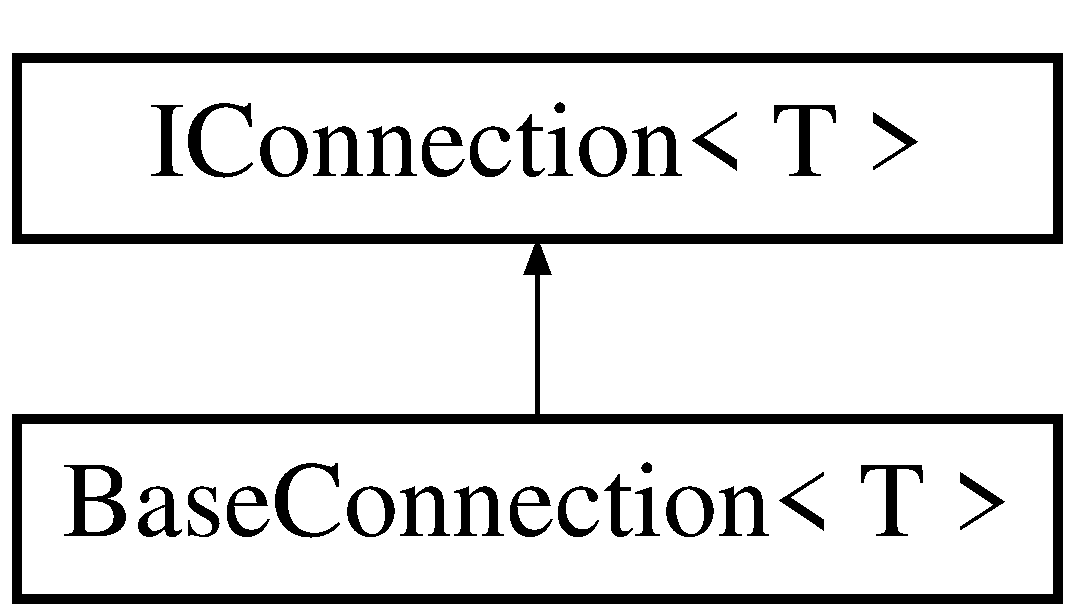
\includegraphics[height=2.000000cm]{class_base_connection}
\end{center}
\end{figure}
\subsection*{Public Member Functions}
\begin{DoxyCompactItemize}
\item 
\mbox{\hyperlink{class_base_connection_a37e4aa9ebfd71b7b5916a2d82bd58a14}{Base\+Connection}} (T from, T to)
\item 
virtual float \mbox{\hyperlink{class_base_connection_a3f2351e9bf997450cca8f64e1e32337a}{Get\+Cost}} ()
\begin{DoxyCompactList}\small\item\em Returns the non-\/negative cost of the connection \end{DoxyCompactList}\item 
T \mbox{\hyperlink{class_base_connection_a45f52b2a297e6ac3a1bca5b5b0d80b89}{Get\+From\+Node}} ()
\begin{DoxyCompactList}\small\item\em Returns the id of the node that this connection from. \end{DoxyCompactList}\item 
T \mbox{\hyperlink{class_base_connection_ad6baf1f89a5abd5f860e1ec58244aab7}{Get\+To\+Node}} ()
\begin{DoxyCompactList}\small\item\em Returns the id of the node that this connection leads to. \end{DoxyCompactList}\item 
bool \mbox{\hyperlink{class_base_connection_a94d80620b77e0c9c0afdcef31ade9196}{Has\+Node}} (T t)
\end{DoxyCompactItemize}
\subsection*{Public Attributes}
\begin{DoxyCompactItemize}
\item 
float \mbox{\hyperlink{class_base_connection_a7dd0468ec0dfbd6dfdcb0ea54516f361}{cost}} = 1
\end{DoxyCompactItemize}
\subsection*{Protected Attributes}
\begin{DoxyCompactItemize}
\item 
T \mbox{\hyperlink{class_base_connection_a30ae67c939f355a10a00539e1db5f6f7}{from\+Node}}
\item 
T \mbox{\hyperlink{class_base_connection_a2c37f6dab5d3d2779dfe3cf8923495e1}{to\+Node}}
\end{DoxyCompactItemize}


\subsection{Constructor \& Destructor Documentation}
\mbox{\Hypertarget{class_base_connection_a37e4aa9ebfd71b7b5916a2d82bd58a14}\label{class_base_connection_a37e4aa9ebfd71b7b5916a2d82bd58a14}} 
\index{Base\+Connection@{Base\+Connection}!Base\+Connection@{Base\+Connection}}
\index{Base\+Connection@{Base\+Connection}!Base\+Connection@{Base\+Connection}}
\subsubsection{\texorpdfstring{Base\+Connection()}{BaseConnection()}}
{\footnotesize\ttfamily \mbox{\hyperlink{class_base_connection}{Base\+Connection}}$<$ T $>$.\mbox{\hyperlink{class_base_connection}{Base\+Connection}} (\begin{DoxyParamCaption}\item[{T}]{from,  }\item[{T}]{to }\end{DoxyParamCaption})}



\subsection{Member Function Documentation}
\mbox{\Hypertarget{class_base_connection_a3f2351e9bf997450cca8f64e1e32337a}\label{class_base_connection_a3f2351e9bf997450cca8f64e1e32337a}} 
\index{Base\+Connection@{Base\+Connection}!Get\+Cost@{Get\+Cost}}
\index{Get\+Cost@{Get\+Cost}!Base\+Connection@{Base\+Connection}}
\subsubsection{\texorpdfstring{Get\+Cost()}{GetCost()}}
{\footnotesize\ttfamily virtual float \mbox{\hyperlink{class_base_connection}{Base\+Connection}}$<$ T $>$.Get\+Cost (\begin{DoxyParamCaption}{ }\end{DoxyParamCaption})\hspace{0.3cm}{\ttfamily [virtual]}}



Returns the non-\/negative cost of the connection 

\begin{DoxyReturn}{Returns}

\end{DoxyReturn}


Implements \mbox{\hyperlink{interface_i_connection_adf42d8cf17bee3b3b1ee299d6f9de1df}{I\+Connection$<$ T $>$}}.



Reimplemented in \mbox{\hyperlink{class_node_edge_aa2eb53bd74c21ecc54af55568af1b6cc}{Node\+Edge}}.

\mbox{\Hypertarget{class_base_connection_a45f52b2a297e6ac3a1bca5b5b0d80b89}\label{class_base_connection_a45f52b2a297e6ac3a1bca5b5b0d80b89}} 
\index{Base\+Connection@{Base\+Connection}!Get\+From\+Node@{Get\+From\+Node}}
\index{Get\+From\+Node@{Get\+From\+Node}!Base\+Connection@{Base\+Connection}}
\subsubsection{\texorpdfstring{Get\+From\+Node()}{GetFromNode()}}
{\footnotesize\ttfamily T \mbox{\hyperlink{class_base_connection}{Base\+Connection}}$<$ T $>$.Get\+From\+Node (\begin{DoxyParamCaption}{ }\end{DoxyParamCaption})}



Returns the id of the node that this connection from. 

\begin{DoxyReturn}{Returns}

\end{DoxyReturn}


Implements \mbox{\hyperlink{interface_i_connection_acecfce42b26af8f2f83e3a806edc6910}{I\+Connection$<$ T $>$}}.

\mbox{\Hypertarget{class_base_connection_ad6baf1f89a5abd5f860e1ec58244aab7}\label{class_base_connection_ad6baf1f89a5abd5f860e1ec58244aab7}} 
\index{Base\+Connection@{Base\+Connection}!Get\+To\+Node@{Get\+To\+Node}}
\index{Get\+To\+Node@{Get\+To\+Node}!Base\+Connection@{Base\+Connection}}
\subsubsection{\texorpdfstring{Get\+To\+Node()}{GetToNode()}}
{\footnotesize\ttfamily T \mbox{\hyperlink{class_base_connection}{Base\+Connection}}$<$ T $>$.Get\+To\+Node (\begin{DoxyParamCaption}{ }\end{DoxyParamCaption})}



Returns the id of the node that this connection leads to. 

\begin{DoxyReturn}{Returns}

\end{DoxyReturn}


Implements \mbox{\hyperlink{interface_i_connection_a738b6e5b2c2620e9e4a8a3e07fe85b52}{I\+Connection$<$ T $>$}}.

\mbox{\Hypertarget{class_base_connection_a94d80620b77e0c9c0afdcef31ade9196}\label{class_base_connection_a94d80620b77e0c9c0afdcef31ade9196}} 
\index{Base\+Connection@{Base\+Connection}!Has\+Node@{Has\+Node}}
\index{Has\+Node@{Has\+Node}!Base\+Connection@{Base\+Connection}}
\subsubsection{\texorpdfstring{Has\+Node()}{HasNode()}}
{\footnotesize\ttfamily bool \mbox{\hyperlink{class_base_connection}{Base\+Connection}}$<$ T $>$.Has\+Node (\begin{DoxyParamCaption}\item[{T}]{t }\end{DoxyParamCaption})}



Implements \mbox{\hyperlink{interface_i_connection_a0789fc3877953a8da47402b986c8469d}{I\+Connection$<$ T $>$}}.



\subsection{Member Data Documentation}
\mbox{\Hypertarget{class_base_connection_a7dd0468ec0dfbd6dfdcb0ea54516f361}\label{class_base_connection_a7dd0468ec0dfbd6dfdcb0ea54516f361}} 
\index{Base\+Connection@{Base\+Connection}!cost@{cost}}
\index{cost@{cost}!Base\+Connection@{Base\+Connection}}
\subsubsection{\texorpdfstring{cost}{cost}}
{\footnotesize\ttfamily float \mbox{\hyperlink{class_base_connection}{Base\+Connection}}$<$ T $>$.cost = 1}

\mbox{\Hypertarget{class_base_connection_a30ae67c939f355a10a00539e1db5f6f7}\label{class_base_connection_a30ae67c939f355a10a00539e1db5f6f7}} 
\index{Base\+Connection@{Base\+Connection}!from\+Node@{from\+Node}}
\index{from\+Node@{from\+Node}!Base\+Connection@{Base\+Connection}}
\subsubsection{\texorpdfstring{from\+Node}{fromNode}}
{\footnotesize\ttfamily T \mbox{\hyperlink{class_base_connection}{Base\+Connection}}$<$ T $>$.from\+Node\hspace{0.3cm}{\ttfamily [protected]}}

\mbox{\Hypertarget{class_base_connection_a2c37f6dab5d3d2779dfe3cf8923495e1}\label{class_base_connection_a2c37f6dab5d3d2779dfe3cf8923495e1}} 
\index{Base\+Connection@{Base\+Connection}!to\+Node@{to\+Node}}
\index{to\+Node@{to\+Node}!Base\+Connection@{Base\+Connection}}
\subsubsection{\texorpdfstring{to\+Node}{toNode}}
{\footnotesize\ttfamily T \mbox{\hyperlink{class_base_connection}{Base\+Connection}}$<$ T $>$.to\+Node\hspace{0.3cm}{\ttfamily [protected]}}



The documentation for this class was generated from the following file\+:\begin{DoxyCompactItemize}
\item 
/\+Users/sabienambrose/\+Documents/\+Coding/\+Unity\+Mechanical\+Turk/\+Mechanical\+Turk/\+Assets/\+Scripts/\+Util/\+Containers/\+Graphs/\mbox{\hyperlink{_base_connection_8cs}{Base\+Connection.\+cs}}\end{DoxyCompactItemize}

\hypertarget{class_biome_generator}{}\section{Biome\+Generator Class Reference}
\label{class_biome_generator}\index{Biome\+Generator@{Biome\+Generator}}
Inheritance diagram for Biome\+Generator\+:\begin{figure}[H]
\begin{center}
\leavevmode
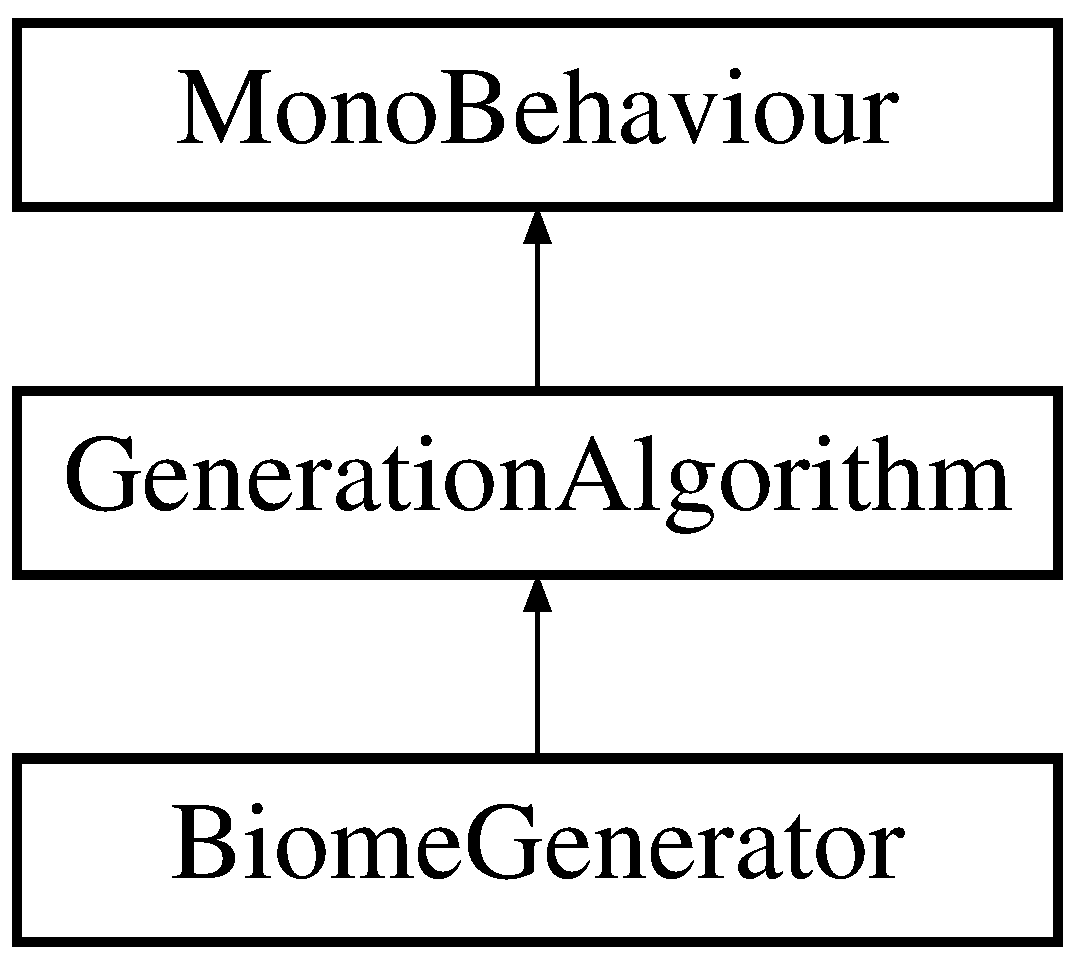
\includegraphics[height=3.000000cm]{class_biome_generator}
\end{center}
\end{figure}
\subsection*{Public Member Functions}
\begin{DoxyCompactItemize}
\item 
override bool \mbox{\hyperlink{class_biome_generator_abe3d21283eef52d4c3ae631178ab69fc}{Can\+Generate}} ()
\begin{DoxyCompactList}\small\item\em Checks to see if generation prerequisites are met. \end{DoxyCompactList}\item 
override void \mbox{\hyperlink{class_biome_generator_aa1df38909c58ff7112ebfd285e65f6c0}{Setup}} ()
\begin{DoxyCompactList}\small\item\em Collects any prerequisites for generation. \end{DoxyCompactList}\item 
override void \mbox{\hyperlink{class_biome_generator_ac8ac31b6e0276662994f0cd143457fdb}{Generate}} ()
\item 
Color \mbox{[}$\,$\mbox{]} \mbox{\hyperlink{class_biome_generator_ad1c3b877b0dde5621250e5ca3c78446a}{Get\+Color\+Map}} ()
\item 
int \mbox{\hyperlink{class_biome_generator_aa4113331412728f686a99dfebf78a42e}{Find\+Best\+Terrain}} (float height\+Value)
\end{DoxyCompactItemize}
\subsection*{Public Attributes}
\begin{DoxyCompactItemize}
\item 
\mbox{\hyperlink{struct_terrain_type}{Terrain\+Type}} \mbox{[}$\,$\mbox{]} \mbox{\hyperlink{class_biome_generator_a3ff1f2229659aaf0008f4c3ffd286efe}{biome\+Types}}
\item 
\mbox{\hyperlink{class_noise_map}{Noise\+Map}} \mbox{\hyperlink{class_biome_generator_a26984c4131089a2ad1b9f8a2eb2c3e28}{height\+Map}}
\item 
int \mbox{[},\mbox{]} \mbox{\hyperlink{class_biome_generator_a3fed4e888962415d1e2b758c33c45c81}{biome\+Map}}
\end{DoxyCompactItemize}


\subsection{Member Function Documentation}
\mbox{\Hypertarget{class_biome_generator_abe3d21283eef52d4c3ae631178ab69fc}\label{class_biome_generator_abe3d21283eef52d4c3ae631178ab69fc}} 
\index{Biome\+Generator@{Biome\+Generator}!Can\+Generate@{Can\+Generate}}
\index{Can\+Generate@{Can\+Generate}!Biome\+Generator@{Biome\+Generator}}
\subsubsection{\texorpdfstring{Can\+Generate()}{CanGenerate()}}
{\footnotesize\ttfamily override bool Biome\+Generator.\+Can\+Generate (\begin{DoxyParamCaption}{ }\end{DoxyParamCaption})\hspace{0.3cm}{\ttfamily [virtual]}}



Checks to see if generation prerequisites are met. 

\begin{DoxyReturn}{Returns}
true if ready for generation.
\end{DoxyReturn}


Implements \mbox{\hyperlink{class_generation_algorithm_af7d03e24e3b7fecfe2ae43f06915986d}{Generation\+Algorithm}}.

\mbox{\Hypertarget{class_biome_generator_aa4113331412728f686a99dfebf78a42e}\label{class_biome_generator_aa4113331412728f686a99dfebf78a42e}} 
\index{Biome\+Generator@{Biome\+Generator}!Find\+Best\+Terrain@{Find\+Best\+Terrain}}
\index{Find\+Best\+Terrain@{Find\+Best\+Terrain}!Biome\+Generator@{Biome\+Generator}}
\subsubsection{\texorpdfstring{Find\+Best\+Terrain()}{FindBestTerrain()}}
{\footnotesize\ttfamily int Biome\+Generator.\+Find\+Best\+Terrain (\begin{DoxyParamCaption}\item[{float}]{height\+Value }\end{DoxyParamCaption})}

\mbox{\Hypertarget{class_biome_generator_ac8ac31b6e0276662994f0cd143457fdb}\label{class_biome_generator_ac8ac31b6e0276662994f0cd143457fdb}} 
\index{Biome\+Generator@{Biome\+Generator}!Generate@{Generate}}
\index{Generate@{Generate}!Biome\+Generator@{Biome\+Generator}}
\subsubsection{\texorpdfstring{Generate()}{Generate()}}
{\footnotesize\ttfamily override void Biome\+Generator.\+Generate (\begin{DoxyParamCaption}{ }\end{DoxyParamCaption})\hspace{0.3cm}{\ttfamily [virtual]}}



Implements \mbox{\hyperlink{class_generation_algorithm_ac2df20f7751c1b480ab958791d5c7d41}{Generation\+Algorithm}}.

\mbox{\Hypertarget{class_biome_generator_ad1c3b877b0dde5621250e5ca3c78446a}\label{class_biome_generator_ad1c3b877b0dde5621250e5ca3c78446a}} 
\index{Biome\+Generator@{Biome\+Generator}!Get\+Color\+Map@{Get\+Color\+Map}}
\index{Get\+Color\+Map@{Get\+Color\+Map}!Biome\+Generator@{Biome\+Generator}}
\subsubsection{\texorpdfstring{Get\+Color\+Map()}{GetColorMap()}}
{\footnotesize\ttfamily Color \mbox{[}$\,$\mbox{]} Biome\+Generator.\+Get\+Color\+Map (\begin{DoxyParamCaption}{ }\end{DoxyParamCaption})}

\mbox{\Hypertarget{class_biome_generator_aa1df38909c58ff7112ebfd285e65f6c0}\label{class_biome_generator_aa1df38909c58ff7112ebfd285e65f6c0}} 
\index{Biome\+Generator@{Biome\+Generator}!Setup@{Setup}}
\index{Setup@{Setup}!Biome\+Generator@{Biome\+Generator}}
\subsubsection{\texorpdfstring{Setup()}{Setup()}}
{\footnotesize\ttfamily override void Biome\+Generator.\+Setup (\begin{DoxyParamCaption}{ }\end{DoxyParamCaption})\hspace{0.3cm}{\ttfamily [virtual]}}



Collects any prerequisites for generation. 



Implements \mbox{\hyperlink{class_generation_algorithm_a5e891b08f0c1d8f4ccc9ad06667691ec}{Generation\+Algorithm}}.



\subsection{Member Data Documentation}
\mbox{\Hypertarget{class_biome_generator_a3fed4e888962415d1e2b758c33c45c81}\label{class_biome_generator_a3fed4e888962415d1e2b758c33c45c81}} 
\index{Biome\+Generator@{Biome\+Generator}!biome\+Map@{biome\+Map}}
\index{biome\+Map@{biome\+Map}!Biome\+Generator@{Biome\+Generator}}
\subsubsection{\texorpdfstring{biome\+Map}{biomeMap}}
{\footnotesize\ttfamily int \mbox{[},\mbox{]} Biome\+Generator.\+biome\+Map}

\mbox{\Hypertarget{class_biome_generator_a3ff1f2229659aaf0008f4c3ffd286efe}\label{class_biome_generator_a3ff1f2229659aaf0008f4c3ffd286efe}} 
\index{Biome\+Generator@{Biome\+Generator}!biome\+Types@{biome\+Types}}
\index{biome\+Types@{biome\+Types}!Biome\+Generator@{Biome\+Generator}}
\subsubsection{\texorpdfstring{biome\+Types}{biomeTypes}}
{\footnotesize\ttfamily \mbox{\hyperlink{struct_terrain_type}{Terrain\+Type}} \mbox{[}$\,$\mbox{]} Biome\+Generator.\+biome\+Types}

\mbox{\Hypertarget{class_biome_generator_a26984c4131089a2ad1b9f8a2eb2c3e28}\label{class_biome_generator_a26984c4131089a2ad1b9f8a2eb2c3e28}} 
\index{Biome\+Generator@{Biome\+Generator}!height\+Map@{height\+Map}}
\index{height\+Map@{height\+Map}!Biome\+Generator@{Biome\+Generator}}
\subsubsection{\texorpdfstring{height\+Map}{heightMap}}
{\footnotesize\ttfamily \mbox{\hyperlink{class_noise_map}{Noise\+Map}} Biome\+Generator.\+height\+Map}



The documentation for this class was generated from the following file\+:\begin{DoxyCompactItemize}
\item 
/\+Users/sabienambrose/\+Documents/\+Coding/\+Unity\+Mechanical\+Turk/\+Mechanical\+Turk/\+Assets/\+Scripts/\+Generation/\mbox{\hyperlink{_biome_generator_8cs}{Biome\+Generator.\+cs}}\end{DoxyCompactItemize}

\hypertarget{struct_circum_circ}{}\section{Circum\+Circ Struct Reference}
\label{struct_circum_circ}\index{Circum\+Circ@{Circum\+Circ}}
\subsection*{Public Member Functions}
\begin{DoxyCompactItemize}
\item 
\mbox{\hyperlink{struct_circum_circ_ada56c128b52d0eabfc4ef19de0490589}{Circum\+Circ}} (Vector2 C, float r)
\item 
override string \mbox{\hyperlink{struct_circum_circ_ae51a3357893dd35882d55c01e8784d21}{To\+String}} ()
\end{DoxyCompactItemize}
\subsection*{Public Attributes}
\begin{DoxyCompactItemize}
\item 
Vector2 \mbox{\hyperlink{struct_circum_circ_ac0b08155df88d5ebfe7970e94bba4adf}{Center}}
\item 
float \mbox{\hyperlink{struct_circum_circ_a135edc470aa3698901aad8e662c43f02}{Radius}}
\end{DoxyCompactItemize}


\subsection{Constructor \& Destructor Documentation}
\mbox{\Hypertarget{struct_circum_circ_ada56c128b52d0eabfc4ef19de0490589}\label{struct_circum_circ_ada56c128b52d0eabfc4ef19de0490589}} 
\index{Circum\+Circ@{Circum\+Circ}!Circum\+Circ@{Circum\+Circ}}
\index{Circum\+Circ@{Circum\+Circ}!Circum\+Circ@{Circum\+Circ}}
\subsubsection{\texorpdfstring{Circum\+Circ()}{CircumCirc()}}
{\footnotesize\ttfamily Circum\+Circ.\+Circum\+Circ (\begin{DoxyParamCaption}\item[{Vector2}]{C,  }\item[{float}]{r }\end{DoxyParamCaption})}



\subsection{Member Function Documentation}
\mbox{\Hypertarget{struct_circum_circ_ae51a3357893dd35882d55c01e8784d21}\label{struct_circum_circ_ae51a3357893dd35882d55c01e8784d21}} 
\index{Circum\+Circ@{Circum\+Circ}!To\+String@{To\+String}}
\index{To\+String@{To\+String}!Circum\+Circ@{Circum\+Circ}}
\subsubsection{\texorpdfstring{To\+String()}{ToString()}}
{\footnotesize\ttfamily override string Circum\+Circ.\+To\+String (\begin{DoxyParamCaption}{ }\end{DoxyParamCaption})}



\subsection{Member Data Documentation}
\mbox{\Hypertarget{struct_circum_circ_ac0b08155df88d5ebfe7970e94bba4adf}\label{struct_circum_circ_ac0b08155df88d5ebfe7970e94bba4adf}} 
\index{Circum\+Circ@{Circum\+Circ}!Center@{Center}}
\index{Center@{Center}!Circum\+Circ@{Circum\+Circ}}
\subsubsection{\texorpdfstring{Center}{Center}}
{\footnotesize\ttfamily Vector2 Circum\+Circ.\+Center}

\mbox{\Hypertarget{struct_circum_circ_a135edc470aa3698901aad8e662c43f02}\label{struct_circum_circ_a135edc470aa3698901aad8e662c43f02}} 
\index{Circum\+Circ@{Circum\+Circ}!Radius@{Radius}}
\index{Radius@{Radius}!Circum\+Circ@{Circum\+Circ}}
\subsubsection{\texorpdfstring{Radius}{Radius}}
{\footnotesize\ttfamily float Circum\+Circ.\+Radius}



The documentation for this struct was generated from the following file\+:\begin{DoxyCompactItemize}
\item 
/\+Users/sabienambrose/\+Documents/\+Coding/\+Unity\+Mechanical\+Turk/\+Mechanical\+Turk/\+Assets/\+Scripts/\+Util/\+Containers/\+Graphs/\+Triangle\+Graphs/\mbox{\hyperlink{_delaunay_triangulation_8cs}{Delaunay\+Triangulation.\+cs}}\end{DoxyCompactItemize}

\hypertarget{class_city_generator}{}\section{City\+Generator Class Reference}
\label{class_city_generator}\index{City\+Generator@{City\+Generator}}
Inheritance diagram for City\+Generator\+:\begin{figure}[H]
\begin{center}
\leavevmode
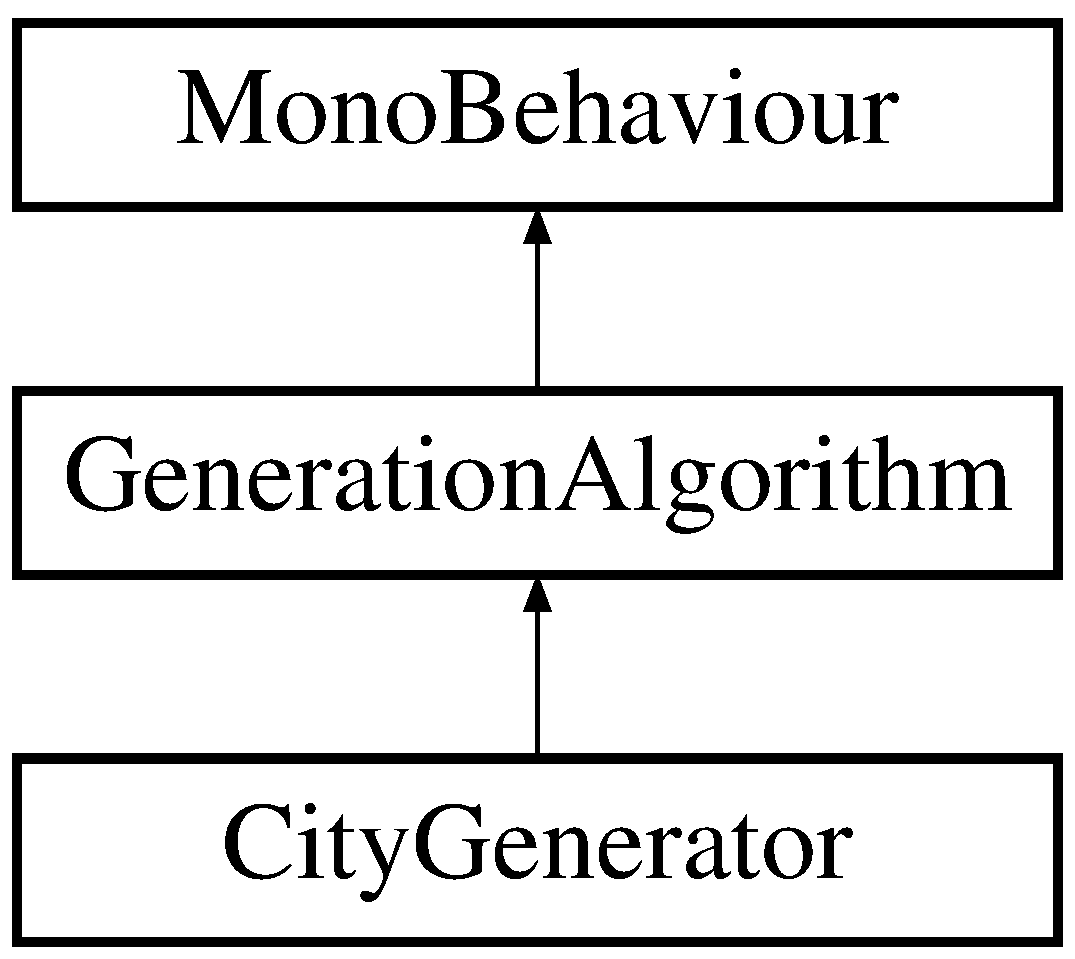
\includegraphics[height=3.000000cm]{class_city_generator}
\end{center}
\end{figure}
\subsection*{Public Member Functions}
\begin{DoxyCompactItemize}
\item 
override bool \mbox{\hyperlink{class_city_generator_abae83261cf4eea2ed07339b644ed13af}{Can\+Generate}} ()
\begin{DoxyCompactList}\small\item\em Checks to see if generation prerequisites are met. \end{DoxyCompactList}\item 
override void \mbox{\hyperlink{class_city_generator_a1b17b4a2ea1d8a4cc1b320829da286ae}{Setup}} ()
\begin{DoxyCompactList}\small\item\em Collects any prerequisites for generation. \end{DoxyCompactList}\item 
override void \mbox{\hyperlink{class_city_generator_aa80ad8d8d723fd17f6bf9a4fe89dec4f}{Generate}} ()
\end{DoxyCompactItemize}
\subsection*{Public Attributes}
\begin{DoxyCompactItemize}
\item 
\mbox{\hyperlink{class_noise_map}{Noise\+Map}} \mbox{\hyperlink{class_city_generator_a41f981122cd74ff6758e7b4dda236085}{height\+Map}}
\item 
\mbox{\hyperlink{class_poly_grid}{Poly\+Grid}} \mbox{\hyperlink{class_city_generator_a9c2dcf98212de701d637f3f3d39214c9}{poly\+Grid}}
\item 
Game\+Object \mbox{[}$\,$\mbox{]} \mbox{\hyperlink{class_city_generator_aa3865cc4ee840dc1d72701093efa4c24}{L\+O\+D\+\_\+0\+\_\+\+Prefabs}} = new Game\+Object\mbox{[}3\mbox{]}
\end{DoxyCompactItemize}


\subsection{Member Function Documentation}
\mbox{\Hypertarget{class_city_generator_abae83261cf4eea2ed07339b644ed13af}\label{class_city_generator_abae83261cf4eea2ed07339b644ed13af}} 
\index{City\+Generator@{City\+Generator}!Can\+Generate@{Can\+Generate}}
\index{Can\+Generate@{Can\+Generate}!City\+Generator@{City\+Generator}}
\subsubsection{\texorpdfstring{Can\+Generate()}{CanGenerate()}}
{\footnotesize\ttfamily override bool City\+Generator.\+Can\+Generate (\begin{DoxyParamCaption}{ }\end{DoxyParamCaption})\hspace{0.3cm}{\ttfamily [virtual]}}



Checks to see if generation prerequisites are met. 

\begin{DoxyReturn}{Returns}
true if ready for generation.
\end{DoxyReturn}


Implements \mbox{\hyperlink{class_generation_algorithm_af7d03e24e3b7fecfe2ae43f06915986d}{Generation\+Algorithm}}.

\mbox{\Hypertarget{class_city_generator_aa80ad8d8d723fd17f6bf9a4fe89dec4f}\label{class_city_generator_aa80ad8d8d723fd17f6bf9a4fe89dec4f}} 
\index{City\+Generator@{City\+Generator}!Generate@{Generate}}
\index{Generate@{Generate}!City\+Generator@{City\+Generator}}
\subsubsection{\texorpdfstring{Generate()}{Generate()}}
{\footnotesize\ttfamily override void City\+Generator.\+Generate (\begin{DoxyParamCaption}{ }\end{DoxyParamCaption})\hspace{0.3cm}{\ttfamily [virtual]}}



Implements \mbox{\hyperlink{class_generation_algorithm_ac2df20f7751c1b480ab958791d5c7d41}{Generation\+Algorithm}}.

\mbox{\Hypertarget{class_city_generator_a1b17b4a2ea1d8a4cc1b320829da286ae}\label{class_city_generator_a1b17b4a2ea1d8a4cc1b320829da286ae}} 
\index{City\+Generator@{City\+Generator}!Setup@{Setup}}
\index{Setup@{Setup}!City\+Generator@{City\+Generator}}
\subsubsection{\texorpdfstring{Setup()}{Setup()}}
{\footnotesize\ttfamily override void City\+Generator.\+Setup (\begin{DoxyParamCaption}{ }\end{DoxyParamCaption})\hspace{0.3cm}{\ttfamily [virtual]}}



Collects any prerequisites for generation. 



Implements \mbox{\hyperlink{class_generation_algorithm_a5e891b08f0c1d8f4ccc9ad06667691ec}{Generation\+Algorithm}}.



\subsection{Member Data Documentation}
\mbox{\Hypertarget{class_city_generator_a41f981122cd74ff6758e7b4dda236085}\label{class_city_generator_a41f981122cd74ff6758e7b4dda236085}} 
\index{City\+Generator@{City\+Generator}!height\+Map@{height\+Map}}
\index{height\+Map@{height\+Map}!City\+Generator@{City\+Generator}}
\subsubsection{\texorpdfstring{height\+Map}{heightMap}}
{\footnotesize\ttfamily \mbox{\hyperlink{class_noise_map}{Noise\+Map}} City\+Generator.\+height\+Map}

\mbox{\Hypertarget{class_city_generator_aa3865cc4ee840dc1d72701093efa4c24}\label{class_city_generator_aa3865cc4ee840dc1d72701093efa4c24}} 
\index{City\+Generator@{City\+Generator}!L\+O\+D\+\_\+0\+\_\+\+Prefabs@{L\+O\+D\+\_\+0\+\_\+\+Prefabs}}
\index{L\+O\+D\+\_\+0\+\_\+\+Prefabs@{L\+O\+D\+\_\+0\+\_\+\+Prefabs}!City\+Generator@{City\+Generator}}
\subsubsection{\texorpdfstring{L\+O\+D\+\_\+0\+\_\+\+Prefabs}{LOD\_0\_Prefabs}}
{\footnotesize\ttfamily Game\+Object \mbox{[}$\,$\mbox{]} City\+Generator.\+L\+O\+D\+\_\+0\+\_\+\+Prefabs = new Game\+Object\mbox{[}3\mbox{]}}

\mbox{\Hypertarget{class_city_generator_a9c2dcf98212de701d637f3f3d39214c9}\label{class_city_generator_a9c2dcf98212de701d637f3f3d39214c9}} 
\index{City\+Generator@{City\+Generator}!poly\+Grid@{poly\+Grid}}
\index{poly\+Grid@{poly\+Grid}!City\+Generator@{City\+Generator}}
\subsubsection{\texorpdfstring{poly\+Grid}{polyGrid}}
{\footnotesize\ttfamily \mbox{\hyperlink{class_poly_grid}{Poly\+Grid}} City\+Generator.\+poly\+Grid}



The documentation for this class was generated from the following file\+:\begin{DoxyCompactItemize}
\item 
/\+Users/sabienambrose/\+Documents/\+Coding/\+Unity\+Mechanical\+Turk/\+Mechanical\+Turk/\+Assets/\+Scripts/\+Framework/\+Generation/\mbox{\hyperlink{_city_generator_8cs}{City\+Generator.\+cs}}\end{DoxyCompactItemize}

\hypertarget{class_clutter_placement}{}\section{Clutter\+Placement Class Reference}
\label{class_clutter_placement}\index{Clutter\+Placement@{Clutter\+Placement}}
Inheritance diagram for Clutter\+Placement\+:\begin{figure}[H]
\begin{center}
\leavevmode
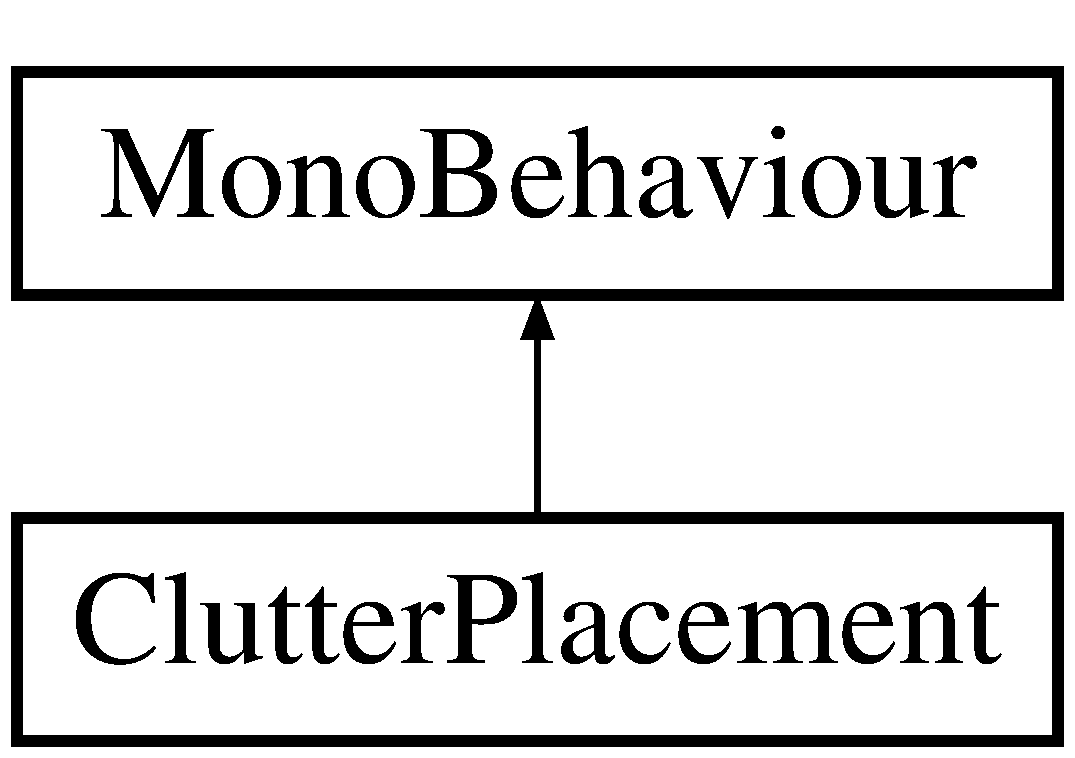
\includegraphics[height=2.000000cm]{class_clutter_placement}
\end{center}
\end{figure}
\subsection*{Public Member Functions}
\begin{DoxyCompactItemize}
\item 
void \mbox{\hyperlink{class_clutter_placement_ab27c08059209c83e0978398f3bfdde9b}{place\+Clutter}} ()
\item 
void \mbox{\hyperlink{class_clutter_placement_a04a7692842800b021ea68e6be3ed5a4c}{clear\+Clutter}} ()
\item 
Game\+Object \mbox{\hyperlink{class_clutter_placement_a00508e28f3977a7622a11653cb625f65}{Get\+Random\+Clutter}} ()
\end{DoxyCompactItemize}
\subsection*{Public Attributes}
\begin{DoxyCompactItemize}
\item 
Game\+Object \mbox{[}$\,$\mbox{]} \mbox{\hyperlink{class_clutter_placement_a0438378166fab8abdbb483d4252e181f}{clutter\+Prefabs}}
\item 
\mbox{\hyperlink{class_point_generator}{Point\+Generator}} \mbox{\hyperlink{class_clutter_placement_a954b2af9e4dcc7ffe61b63c9f1b7a873}{point\+Generator}}
\item 
List$<$ Game\+Object $>$ \mbox{\hyperlink{class_clutter_placement_ad9f568266937efd7a7938371c7179e4a}{spawned\+Clutter}}
\item 
Mesh\+Filter \mbox{\hyperlink{class_clutter_placement_a28d25417ea666507f5a68e5c789ac903}{map\+Mesh\+Filter}}
\end{DoxyCompactItemize}


\subsection{Member Function Documentation}
\mbox{\Hypertarget{class_clutter_placement_a04a7692842800b021ea68e6be3ed5a4c}\label{class_clutter_placement_a04a7692842800b021ea68e6be3ed5a4c}} 
\index{Clutter\+Placement@{Clutter\+Placement}!clear\+Clutter@{clear\+Clutter}}
\index{clear\+Clutter@{clear\+Clutter}!Clutter\+Placement@{Clutter\+Placement}}
\subsubsection{\texorpdfstring{clear\+Clutter()}{clearClutter()}}
{\footnotesize\ttfamily void Clutter\+Placement.\+clear\+Clutter (\begin{DoxyParamCaption}{ }\end{DoxyParamCaption})}

\mbox{\Hypertarget{class_clutter_placement_a00508e28f3977a7622a11653cb625f65}\label{class_clutter_placement_a00508e28f3977a7622a11653cb625f65}} 
\index{Clutter\+Placement@{Clutter\+Placement}!Get\+Random\+Clutter@{Get\+Random\+Clutter}}
\index{Get\+Random\+Clutter@{Get\+Random\+Clutter}!Clutter\+Placement@{Clutter\+Placement}}
\subsubsection{\texorpdfstring{Get\+Random\+Clutter()}{GetRandomClutter()}}
{\footnotesize\ttfamily Game\+Object Clutter\+Placement.\+Get\+Random\+Clutter (\begin{DoxyParamCaption}{ }\end{DoxyParamCaption})}

\mbox{\Hypertarget{class_clutter_placement_ab27c08059209c83e0978398f3bfdde9b}\label{class_clutter_placement_ab27c08059209c83e0978398f3bfdde9b}} 
\index{Clutter\+Placement@{Clutter\+Placement}!place\+Clutter@{place\+Clutter}}
\index{place\+Clutter@{place\+Clutter}!Clutter\+Placement@{Clutter\+Placement}}
\subsubsection{\texorpdfstring{place\+Clutter()}{placeClutter()}}
{\footnotesize\ttfamily void Clutter\+Placement.\+place\+Clutter (\begin{DoxyParamCaption}{ }\end{DoxyParamCaption})}



\subsection{Member Data Documentation}
\mbox{\Hypertarget{class_clutter_placement_a0438378166fab8abdbb483d4252e181f}\label{class_clutter_placement_a0438378166fab8abdbb483d4252e181f}} 
\index{Clutter\+Placement@{Clutter\+Placement}!clutter\+Prefabs@{clutter\+Prefabs}}
\index{clutter\+Prefabs@{clutter\+Prefabs}!Clutter\+Placement@{Clutter\+Placement}}
\subsubsection{\texorpdfstring{clutter\+Prefabs}{clutterPrefabs}}
{\footnotesize\ttfamily Game\+Object \mbox{[}$\,$\mbox{]} Clutter\+Placement.\+clutter\+Prefabs}

\mbox{\Hypertarget{class_clutter_placement_a28d25417ea666507f5a68e5c789ac903}\label{class_clutter_placement_a28d25417ea666507f5a68e5c789ac903}} 
\index{Clutter\+Placement@{Clutter\+Placement}!map\+Mesh\+Filter@{map\+Mesh\+Filter}}
\index{map\+Mesh\+Filter@{map\+Mesh\+Filter}!Clutter\+Placement@{Clutter\+Placement}}
\subsubsection{\texorpdfstring{map\+Mesh\+Filter}{mapMeshFilter}}
{\footnotesize\ttfamily Mesh\+Filter Clutter\+Placement.\+map\+Mesh\+Filter}

\mbox{\Hypertarget{class_clutter_placement_a954b2af9e4dcc7ffe61b63c9f1b7a873}\label{class_clutter_placement_a954b2af9e4dcc7ffe61b63c9f1b7a873}} 
\index{Clutter\+Placement@{Clutter\+Placement}!point\+Generator@{point\+Generator}}
\index{point\+Generator@{point\+Generator}!Clutter\+Placement@{Clutter\+Placement}}
\subsubsection{\texorpdfstring{point\+Generator}{pointGenerator}}
{\footnotesize\ttfamily \mbox{\hyperlink{class_point_generator}{Point\+Generator}} Clutter\+Placement.\+point\+Generator}

\mbox{\Hypertarget{class_clutter_placement_ad9f568266937efd7a7938371c7179e4a}\label{class_clutter_placement_ad9f568266937efd7a7938371c7179e4a}} 
\index{Clutter\+Placement@{Clutter\+Placement}!spawned\+Clutter@{spawned\+Clutter}}
\index{spawned\+Clutter@{spawned\+Clutter}!Clutter\+Placement@{Clutter\+Placement}}
\subsubsection{\texorpdfstring{spawned\+Clutter}{spawnedClutter}}
{\footnotesize\ttfamily List$<$Game\+Object$>$ Clutter\+Placement.\+spawned\+Clutter}



The documentation for this class was generated from the following file\+:\begin{DoxyCompactItemize}
\item 
/\+Users/sabienambrose/\+Documents/\+Coding/\+Unity\+Mechanical\+Turk/\+Mechanical\+Turk/\+Assets/\+Scripts/\+Generation/\mbox{\hyperlink{_clutter_placement_8cs}{Clutter\+Placement.\+cs}}\end{DoxyCompactItemize}

\hypertarget{class_utility_system_1_1_consideration}{}\section{Utility\+System.\+Consideration Class Reference}
\label{class_utility_system_1_1_consideration}\index{Utility\+System.\+Consideration@{Utility\+System.\+Consideration}}
Inheritance diagram for Utility\+System.\+Consideration\+:\begin{figure}[H]
\begin{center}
\leavevmode
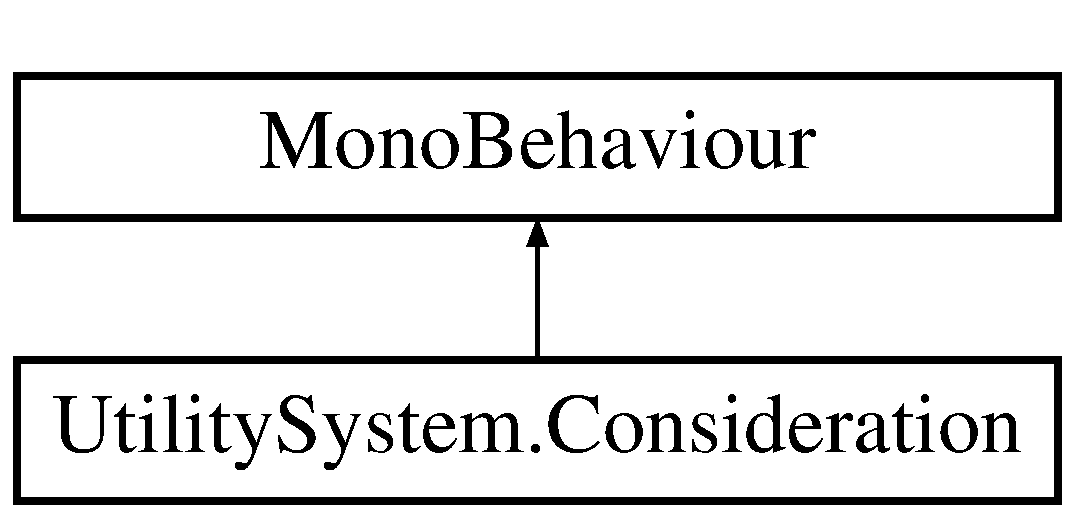
\includegraphics[height=2.000000cm]{class_utility_system_1_1_consideration}
\end{center}
\end{figure}
\subsection*{Public Member Functions}
\begin{DoxyCompactItemize}
\item 
float \mbox{\hyperlink{class_utility_system_1_1_consideration_a06aa9c595c6f247b429028b3d64480b9}{Get\+Float\+Parameter}} (int id)
\item 
virtual float \mbox{\hyperlink{class_utility_system_1_1_consideration_afe926b80ef5f4780b788e6bae93ac89e}{Score}} (\mbox{\hyperlink{class_utility_system_1_1_decision_context}{Decision\+Context}} context)
\item 
abstract float \mbox{\hyperlink{class_utility_system_1_1_consideration_a1340c371b0e917253e906b48b5c3b187}{Score}} (\mbox{\hyperlink{class_utility_system_1_1_decision_context}{Decision\+Context}} context, \mbox{\hyperlink{class_utility_system_1_1_consideration}{Consideration}} c)
\item 
abstract float \mbox{\hyperlink{class_utility_system_1_1_consideration_a899a8fdb51b9e7c82f4a52e8bfb4aba9}{Compute\+Response\+Curve}} (float score)
\end{DoxyCompactItemize}
\subsection*{Public Attributes}
\begin{DoxyCompactItemize}
\item 
string \mbox{\hyperlink{class_utility_system_1_1_consideration_aea5bafaa7a2cb6b8d8dda059e7cbc452}{description}}
\item 
float \mbox{[}$\,$\mbox{]} \mbox{\hyperlink{class_utility_system_1_1_consideration_aab4d2dc6c9084d5684a53b2cc2c7c0c7}{float\+Params}}
\end{DoxyCompactItemize}


\subsection{Member Function Documentation}
\mbox{\Hypertarget{class_utility_system_1_1_consideration_a899a8fdb51b9e7c82f4a52e8bfb4aba9}\label{class_utility_system_1_1_consideration_a899a8fdb51b9e7c82f4a52e8bfb4aba9}} 
\index{Utility\+System\+::\+Consideration@{Utility\+System\+::\+Consideration}!Compute\+Response\+Curve@{Compute\+Response\+Curve}}
\index{Compute\+Response\+Curve@{Compute\+Response\+Curve}!Utility\+System\+::\+Consideration@{Utility\+System\+::\+Consideration}}
\subsubsection{\texorpdfstring{Compute\+Response\+Curve()}{ComputeResponseCurve()}}
{\footnotesize\ttfamily abstract float Utility\+System.\+Consideration.\+Compute\+Response\+Curve (\begin{DoxyParamCaption}\item[{float}]{score }\end{DoxyParamCaption})\hspace{0.3cm}{\ttfamily [pure virtual]}}

\mbox{\Hypertarget{class_utility_system_1_1_consideration_a06aa9c595c6f247b429028b3d64480b9}\label{class_utility_system_1_1_consideration_a06aa9c595c6f247b429028b3d64480b9}} 
\index{Utility\+System\+::\+Consideration@{Utility\+System\+::\+Consideration}!Get\+Float\+Parameter@{Get\+Float\+Parameter}}
\index{Get\+Float\+Parameter@{Get\+Float\+Parameter}!Utility\+System\+::\+Consideration@{Utility\+System\+::\+Consideration}}
\subsubsection{\texorpdfstring{Get\+Float\+Parameter()}{GetFloatParameter()}}
{\footnotesize\ttfamily float Utility\+System.\+Consideration.\+Get\+Float\+Parameter (\begin{DoxyParamCaption}\item[{int}]{id }\end{DoxyParamCaption})}

\mbox{\Hypertarget{class_utility_system_1_1_consideration_afe926b80ef5f4780b788e6bae93ac89e}\label{class_utility_system_1_1_consideration_afe926b80ef5f4780b788e6bae93ac89e}} 
\index{Utility\+System\+::\+Consideration@{Utility\+System\+::\+Consideration}!Score@{Score}}
\index{Score@{Score}!Utility\+System\+::\+Consideration@{Utility\+System\+::\+Consideration}}
\subsubsection{\texorpdfstring{Score()}{Score()}\hspace{0.1cm}{\footnotesize\ttfamily [1/2]}}
{\footnotesize\ttfamily virtual float Utility\+System.\+Consideration.\+Score (\begin{DoxyParamCaption}\item[{\mbox{\hyperlink{class_utility_system_1_1_decision_context}{Decision\+Context}}}]{context }\end{DoxyParamCaption})\hspace{0.3cm}{\ttfamily [virtual]}}

\mbox{\Hypertarget{class_utility_system_1_1_consideration_a1340c371b0e917253e906b48b5c3b187}\label{class_utility_system_1_1_consideration_a1340c371b0e917253e906b48b5c3b187}} 
\index{Utility\+System\+::\+Consideration@{Utility\+System\+::\+Consideration}!Score@{Score}}
\index{Score@{Score}!Utility\+System\+::\+Consideration@{Utility\+System\+::\+Consideration}}
\subsubsection{\texorpdfstring{Score()}{Score()}\hspace{0.1cm}{\footnotesize\ttfamily [2/2]}}
{\footnotesize\ttfamily abstract float Utility\+System.\+Consideration.\+Score (\begin{DoxyParamCaption}\item[{\mbox{\hyperlink{class_utility_system_1_1_decision_context}{Decision\+Context}}}]{context,  }\item[{\mbox{\hyperlink{class_utility_system_1_1_consideration}{Consideration}}}]{c }\end{DoxyParamCaption})\hspace{0.3cm}{\ttfamily [pure virtual]}}



\subsection{Member Data Documentation}
\mbox{\Hypertarget{class_utility_system_1_1_consideration_aea5bafaa7a2cb6b8d8dda059e7cbc452}\label{class_utility_system_1_1_consideration_aea5bafaa7a2cb6b8d8dda059e7cbc452}} 
\index{Utility\+System\+::\+Consideration@{Utility\+System\+::\+Consideration}!description@{description}}
\index{description@{description}!Utility\+System\+::\+Consideration@{Utility\+System\+::\+Consideration}}
\subsubsection{\texorpdfstring{description}{description}}
{\footnotesize\ttfamily string Utility\+System.\+Consideration.\+description}

\mbox{\Hypertarget{class_utility_system_1_1_consideration_aab4d2dc6c9084d5684a53b2cc2c7c0c7}\label{class_utility_system_1_1_consideration_aab4d2dc6c9084d5684a53b2cc2c7c0c7}} 
\index{Utility\+System\+::\+Consideration@{Utility\+System\+::\+Consideration}!float\+Params@{float\+Params}}
\index{float\+Params@{float\+Params}!Utility\+System\+::\+Consideration@{Utility\+System\+::\+Consideration}}
\subsubsection{\texorpdfstring{float\+Params}{floatParams}}
{\footnotesize\ttfamily float \mbox{[}$\,$\mbox{]} Utility\+System.\+Consideration.\+float\+Params}



The documentation for this class was generated from the following file\+:\begin{DoxyCompactItemize}
\item 
/\+Users/sabienambrose/\+Documents/\+Coding/\+Unity\+Mechanical\+Turk/\+Mechanical\+Turk/\+Assets/\+Scripts/\+Framework/\+Utility/\mbox{\hyperlink{_consideration_8cs}{Consideration.\+cs}}\end{DoxyCompactItemize}

\hypertarget{class_utility_system_1_1_decision}{}\section{Utility\+System.\+Decision Class Reference}
\label{class_utility_system_1_1_decision}\index{Utility\+System.\+Decision@{Utility\+System.\+Decision}}
Inheritance diagram for Utility\+System.\+Decision\+:\begin{figure}[H]
\begin{center}
\leavevmode
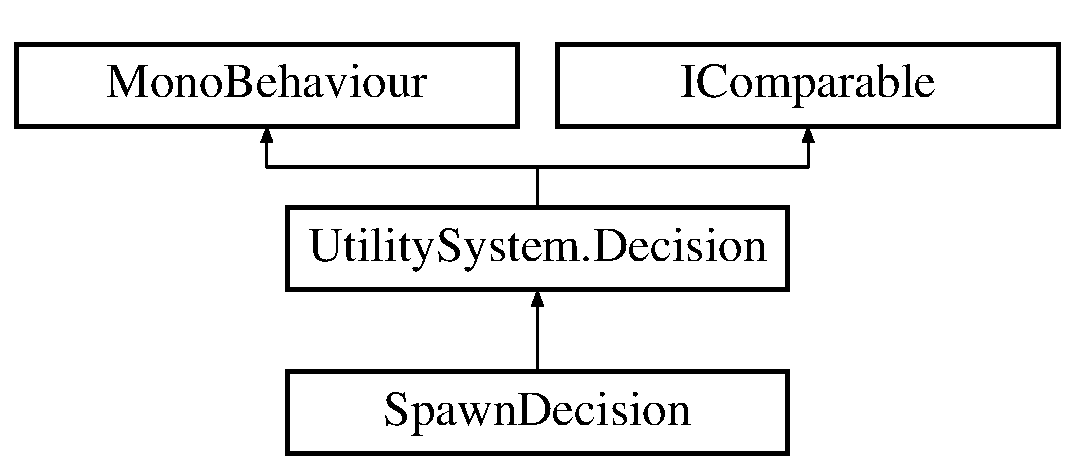
\includegraphics[height=3.000000cm]{class_utility_system_1_1_decision}
\end{center}
\end{figure}
\subsection*{Public Member Functions}
\begin{DoxyCompactItemize}
\item 
abstract \mbox{\hyperlink{class_utility_system_1_1_decision_context}{Decision\+Context}} \mbox{\hyperlink{class_utility_system_1_1_decision_a46ba8cac39f52c630897a24f2bde6b07}{Get\+Context}} ()
\item 
\mbox{\hyperlink{class_utility_system_1_1_decision_score_evaluator}{Decision\+Score\+Evaluator}} \mbox{\hyperlink{class_utility_system_1_1_decision_a7a544c6d16e25998e64d89d510ab7733}{Get\+D\+SE}} ()
\item 
int \mbox{\hyperlink{class_utility_system_1_1_decision_a35c44bfaa350617cb9c18c6961f66ba8}{Compare\+To}} (object obj)
\item 
int \mbox{\hyperlink{class_utility_system_1_1_decision_ae75bc92f152e31288002e8ed1dfa8084}{Compare\+To}} (\mbox{\hyperlink{class_utility_system_1_1_decision}{Decision}} other)
\item 
abstract void \mbox{\hyperlink{class_utility_system_1_1_decision_a055dcaafb617365bc8b16bb9acba6575}{Perform}} ()
\end{DoxyCompactItemize}
\subsection*{Public Attributes}
\begin{DoxyCompactItemize}
\item 
int \mbox{\hyperlink{class_utility_system_1_1_decision_ac898590add80a922e0dea64906a536fc}{id}}
\item 
float \mbox{\hyperlink{class_utility_system_1_1_decision_a26d318a50cfa8b16f3955ae814516b8d}{score}}
\item 
\mbox{\hyperlink{class_utility_system_1_1_decision_score_evaluator}{Decision\+Score\+Evaluator}} \mbox{\hyperlink{class_utility_system_1_1_decision_aed761a6523b0eb1148c743665fa05789}{score\+Evaluator}}
\end{DoxyCompactItemize}


\subsection{Member Function Documentation}
\mbox{\Hypertarget{class_utility_system_1_1_decision_a35c44bfaa350617cb9c18c6961f66ba8}\label{class_utility_system_1_1_decision_a35c44bfaa350617cb9c18c6961f66ba8}} 
\index{Utility\+System\+::\+Decision@{Utility\+System\+::\+Decision}!Compare\+To@{Compare\+To}}
\index{Compare\+To@{Compare\+To}!Utility\+System\+::\+Decision@{Utility\+System\+::\+Decision}}
\subsubsection{\texorpdfstring{Compare\+To()}{CompareTo()}\hspace{0.1cm}{\footnotesize\ttfamily [1/2]}}
{\footnotesize\ttfamily int Utility\+System.\+Decision.\+Compare\+To (\begin{DoxyParamCaption}\item[{object}]{obj }\end{DoxyParamCaption})}

\mbox{\Hypertarget{class_utility_system_1_1_decision_ae75bc92f152e31288002e8ed1dfa8084}\label{class_utility_system_1_1_decision_ae75bc92f152e31288002e8ed1dfa8084}} 
\index{Utility\+System\+::\+Decision@{Utility\+System\+::\+Decision}!Compare\+To@{Compare\+To}}
\index{Compare\+To@{Compare\+To}!Utility\+System\+::\+Decision@{Utility\+System\+::\+Decision}}
\subsubsection{\texorpdfstring{Compare\+To()}{CompareTo()}\hspace{0.1cm}{\footnotesize\ttfamily [2/2]}}
{\footnotesize\ttfamily int Utility\+System.\+Decision.\+Compare\+To (\begin{DoxyParamCaption}\item[{\mbox{\hyperlink{class_utility_system_1_1_decision}{Decision}}}]{other }\end{DoxyParamCaption})}

\mbox{\Hypertarget{class_utility_system_1_1_decision_a46ba8cac39f52c630897a24f2bde6b07}\label{class_utility_system_1_1_decision_a46ba8cac39f52c630897a24f2bde6b07}} 
\index{Utility\+System\+::\+Decision@{Utility\+System\+::\+Decision}!Get\+Context@{Get\+Context}}
\index{Get\+Context@{Get\+Context}!Utility\+System\+::\+Decision@{Utility\+System\+::\+Decision}}
\subsubsection{\texorpdfstring{Get\+Context()}{GetContext()}}
{\footnotesize\ttfamily abstract \mbox{\hyperlink{class_utility_system_1_1_decision_context}{Decision\+Context}} Utility\+System.\+Decision.\+Get\+Context (\begin{DoxyParamCaption}{ }\end{DoxyParamCaption})\hspace{0.3cm}{\ttfamily [pure virtual]}}



Implemented in \mbox{\hyperlink{class_spawn_decision_a8c2019e64b2353e9c0eb314cc0e804d7}{Spawn\+Decision}}.

\mbox{\Hypertarget{class_utility_system_1_1_decision_a7a544c6d16e25998e64d89d510ab7733}\label{class_utility_system_1_1_decision_a7a544c6d16e25998e64d89d510ab7733}} 
\index{Utility\+System\+::\+Decision@{Utility\+System\+::\+Decision}!Get\+D\+SE@{Get\+D\+SE}}
\index{Get\+D\+SE@{Get\+D\+SE}!Utility\+System\+::\+Decision@{Utility\+System\+::\+Decision}}
\subsubsection{\texorpdfstring{Get\+D\+S\+E()}{GetDSE()}}
{\footnotesize\ttfamily \mbox{\hyperlink{class_utility_system_1_1_decision_score_evaluator}{Decision\+Score\+Evaluator}} Utility\+System.\+Decision.\+Get\+D\+SE (\begin{DoxyParamCaption}{ }\end{DoxyParamCaption})}

\mbox{\Hypertarget{class_utility_system_1_1_decision_a055dcaafb617365bc8b16bb9acba6575}\label{class_utility_system_1_1_decision_a055dcaafb617365bc8b16bb9acba6575}} 
\index{Utility\+System\+::\+Decision@{Utility\+System\+::\+Decision}!Perform@{Perform}}
\index{Perform@{Perform}!Utility\+System\+::\+Decision@{Utility\+System\+::\+Decision}}
\subsubsection{\texorpdfstring{Perform()}{Perform()}}
{\footnotesize\ttfamily abstract void Utility\+System.\+Decision.\+Perform (\begin{DoxyParamCaption}{ }\end{DoxyParamCaption})\hspace{0.3cm}{\ttfamily [pure virtual]}}



Implemented in \mbox{\hyperlink{class_spawn_decision_a7f943d8fd313e6a38f26b223e4b4dba7}{Spawn\+Decision}}.



\subsection{Member Data Documentation}
\mbox{\Hypertarget{class_utility_system_1_1_decision_ac898590add80a922e0dea64906a536fc}\label{class_utility_system_1_1_decision_ac898590add80a922e0dea64906a536fc}} 
\index{Utility\+System\+::\+Decision@{Utility\+System\+::\+Decision}!id@{id}}
\index{id@{id}!Utility\+System\+::\+Decision@{Utility\+System\+::\+Decision}}
\subsubsection{\texorpdfstring{id}{id}}
{\footnotesize\ttfamily int Utility\+System.\+Decision.\+id}

\mbox{\Hypertarget{class_utility_system_1_1_decision_a26d318a50cfa8b16f3955ae814516b8d}\label{class_utility_system_1_1_decision_a26d318a50cfa8b16f3955ae814516b8d}} 
\index{Utility\+System\+::\+Decision@{Utility\+System\+::\+Decision}!score@{score}}
\index{score@{score}!Utility\+System\+::\+Decision@{Utility\+System\+::\+Decision}}
\subsubsection{\texorpdfstring{score}{score}}
{\footnotesize\ttfamily float Utility\+System.\+Decision.\+score}

\mbox{\Hypertarget{class_utility_system_1_1_decision_aed761a6523b0eb1148c743665fa05789}\label{class_utility_system_1_1_decision_aed761a6523b0eb1148c743665fa05789}} 
\index{Utility\+System\+::\+Decision@{Utility\+System\+::\+Decision}!score\+Evaluator@{score\+Evaluator}}
\index{score\+Evaluator@{score\+Evaluator}!Utility\+System\+::\+Decision@{Utility\+System\+::\+Decision}}
\subsubsection{\texorpdfstring{score\+Evaluator}{scoreEvaluator}}
{\footnotesize\ttfamily \mbox{\hyperlink{class_utility_system_1_1_decision_score_evaluator}{Decision\+Score\+Evaluator}} Utility\+System.\+Decision.\+score\+Evaluator}



The documentation for this class was generated from the following file\+:\begin{DoxyCompactItemize}
\item 
/\+Users/sabienambrose/\+Documents/\+Coding/\+Unity\+Mechanical\+Turk/\+Mechanical\+Turk/\+Assets/\+Scripts/\+Framework/\+Utility/\mbox{\hyperlink{_decision_8cs}{Decision.\+cs}}\end{DoxyCompactItemize}

\hypertarget{class_utility_system_1_1_decision_context}{}\section{Utility\+System.\+Decision\+Context Class Reference}
\label{class_utility_system_1_1_decision_context}\index{Utility\+System.\+Decision\+Context@{Utility\+System.\+Decision\+Context}}
\subsection*{Public Member Functions}
\begin{DoxyCompactItemize}
\item 
\mbox{\hyperlink{class_utility_system_1_1_decision_context_a827706e37081745d5291660508b14df4}{Decision\+Context}} (int decision\+Identifier, Game\+Object intelligence\+Controller, Game\+Object \mbox{\hyperlink{class_utility_system_1_1_decision_context_ad7900272c03f4eca8fcabb15b76fe005}{target\+Object}})
\item 
Game\+Object \mbox{\hyperlink{class_utility_system_1_1_decision_context_a05391232347edeb491c3a918414a2bc7}{Get\+Intelligence}} ()
\item 
virtual float \mbox{\hyperlink{class_utility_system_1_1_decision_context_a811906f5fd74646edde4031a947e81c2}{Get\+Bonus\+Factor}} (\mbox{\hyperlink{class_utility_system_1_1_decision_context}{Decision\+Context}} last\+Decision)
\end{DoxyCompactItemize}
\subsection*{Public Attributes}
\begin{DoxyCompactItemize}
\item 
int \mbox{\hyperlink{class_utility_system_1_1_decision_context_a509cf4a0499cbe43a5758a4324e320ff}{decision\+Id}}
\item 
Game\+Object \mbox{\hyperlink{class_utility_system_1_1_decision_context_aa706423d7e4422c57926689c4f723a5d}{intel\+Object}}
\item 
Game\+Object \mbox{\hyperlink{class_utility_system_1_1_decision_context_ad7900272c03f4eca8fcabb15b76fe005}{target\+Object}}
\end{DoxyCompactItemize}


\subsection{Constructor \& Destructor Documentation}
\mbox{\Hypertarget{class_utility_system_1_1_decision_context_a827706e37081745d5291660508b14df4}\label{class_utility_system_1_1_decision_context_a827706e37081745d5291660508b14df4}} 
\index{Utility\+System\+::\+Decision\+Context@{Utility\+System\+::\+Decision\+Context}!Decision\+Context@{Decision\+Context}}
\index{Decision\+Context@{Decision\+Context}!Utility\+System\+::\+Decision\+Context@{Utility\+System\+::\+Decision\+Context}}
\subsubsection{\texorpdfstring{Decision\+Context()}{DecisionContext()}}
{\footnotesize\ttfamily Utility\+System.\+Decision\+Context.\+Decision\+Context (\begin{DoxyParamCaption}\item[{int}]{decision\+Identifier,  }\item[{Game\+Object}]{intelligence\+Controller,  }\item[{Game\+Object}]{target\+Object }\end{DoxyParamCaption})}



\subsection{Member Function Documentation}
\mbox{\Hypertarget{class_utility_system_1_1_decision_context_a811906f5fd74646edde4031a947e81c2}\label{class_utility_system_1_1_decision_context_a811906f5fd74646edde4031a947e81c2}} 
\index{Utility\+System\+::\+Decision\+Context@{Utility\+System\+::\+Decision\+Context}!Get\+Bonus\+Factor@{Get\+Bonus\+Factor}}
\index{Get\+Bonus\+Factor@{Get\+Bonus\+Factor}!Utility\+System\+::\+Decision\+Context@{Utility\+System\+::\+Decision\+Context}}
\subsubsection{\texorpdfstring{Get\+Bonus\+Factor()}{GetBonusFactor()}}
{\footnotesize\ttfamily virtual float Utility\+System.\+Decision\+Context.\+Get\+Bonus\+Factor (\begin{DoxyParamCaption}\item[{\mbox{\hyperlink{class_utility_system_1_1_decision_context}{Decision\+Context}}}]{last\+Decision }\end{DoxyParamCaption})\hspace{0.3cm}{\ttfamily [virtual]}}

\mbox{\Hypertarget{class_utility_system_1_1_decision_context_a05391232347edeb491c3a918414a2bc7}\label{class_utility_system_1_1_decision_context_a05391232347edeb491c3a918414a2bc7}} 
\index{Utility\+System\+::\+Decision\+Context@{Utility\+System\+::\+Decision\+Context}!Get\+Intelligence@{Get\+Intelligence}}
\index{Get\+Intelligence@{Get\+Intelligence}!Utility\+System\+::\+Decision\+Context@{Utility\+System\+::\+Decision\+Context}}
\subsubsection{\texorpdfstring{Get\+Intelligence()}{GetIntelligence()}}
{\footnotesize\ttfamily Game\+Object Utility\+System.\+Decision\+Context.\+Get\+Intelligence (\begin{DoxyParamCaption}{ }\end{DoxyParamCaption})}



\subsection{Member Data Documentation}
\mbox{\Hypertarget{class_utility_system_1_1_decision_context_a509cf4a0499cbe43a5758a4324e320ff}\label{class_utility_system_1_1_decision_context_a509cf4a0499cbe43a5758a4324e320ff}} 
\index{Utility\+System\+::\+Decision\+Context@{Utility\+System\+::\+Decision\+Context}!decision\+Id@{decision\+Id}}
\index{decision\+Id@{decision\+Id}!Utility\+System\+::\+Decision\+Context@{Utility\+System\+::\+Decision\+Context}}
\subsubsection{\texorpdfstring{decision\+Id}{decisionId}}
{\footnotesize\ttfamily int Utility\+System.\+Decision\+Context.\+decision\+Id}

\mbox{\Hypertarget{class_utility_system_1_1_decision_context_aa706423d7e4422c57926689c4f723a5d}\label{class_utility_system_1_1_decision_context_aa706423d7e4422c57926689c4f723a5d}} 
\index{Utility\+System\+::\+Decision\+Context@{Utility\+System\+::\+Decision\+Context}!intel\+Object@{intel\+Object}}
\index{intel\+Object@{intel\+Object}!Utility\+System\+::\+Decision\+Context@{Utility\+System\+::\+Decision\+Context}}
\subsubsection{\texorpdfstring{intel\+Object}{intelObject}}
{\footnotesize\ttfamily Game\+Object Utility\+System.\+Decision\+Context.\+intel\+Object}

\mbox{\Hypertarget{class_utility_system_1_1_decision_context_ad7900272c03f4eca8fcabb15b76fe005}\label{class_utility_system_1_1_decision_context_ad7900272c03f4eca8fcabb15b76fe005}} 
\index{Utility\+System\+::\+Decision\+Context@{Utility\+System\+::\+Decision\+Context}!target\+Object@{target\+Object}}
\index{target\+Object@{target\+Object}!Utility\+System\+::\+Decision\+Context@{Utility\+System\+::\+Decision\+Context}}
\subsubsection{\texorpdfstring{target\+Object}{targetObject}}
{\footnotesize\ttfamily Game\+Object Utility\+System.\+Decision\+Context.\+target\+Object}



The documentation for this class was generated from the following file\+:\begin{DoxyCompactItemize}
\item 
/\+Users/sabienambrose/\+Documents/\+Coding/\+Unity\+Mechanical\+Turk/\+Mechanical\+Turk/\+Assets/\+Scripts/\+Framework/\+Utility/\mbox{\hyperlink{_decision_context_8cs}{Decision\+Context.\+cs}}\end{DoxyCompactItemize}

\hypertarget{class_utility_system_1_1_decision_maker}{}\section{Utility\+System.\+Decision\+Maker Class Reference}
\label{class_utility_system_1_1_decision_maker}\index{Utility\+System.\+Decision\+Maker@{Utility\+System.\+Decision\+Maker}}
Inheritance diagram for Utility\+System.\+Decision\+Maker\+:\begin{figure}[H]
\begin{center}
\leavevmode
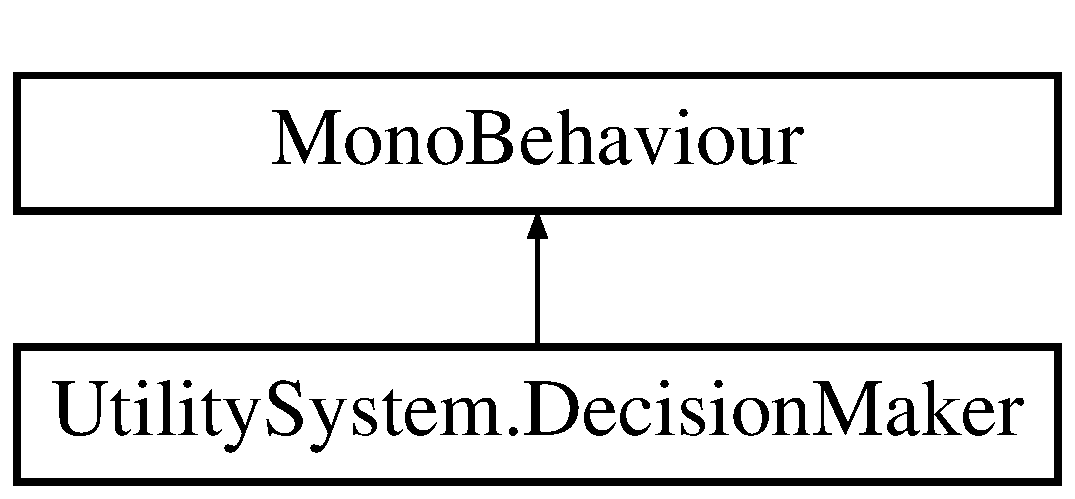
\includegraphics[height=2.000000cm]{class_utility_system_1_1_decision_maker}
\end{center}
\end{figure}
\subsection*{Public Member Functions}
\begin{DoxyCompactItemize}
\item 
void \mbox{\hyperlink{class_utility_system_1_1_decision_maker_a51ccf99d911381b29ca61d69697e93dc}{Perform\+Best\+Decision}} ()
\item 
\mbox{\hyperlink{class_utility_system_1_1_decision}{Decision}} \mbox{\hyperlink{class_utility_system_1_1_decision_maker_a696dfddb4eb31cb1498df83fa6304ae5}{Get\+Best\+Decision}} ()
\item 
void \mbox{\hyperlink{class_utility_system_1_1_decision_maker_ac342e07ac99e8de808e7bbc9faa59a1a}{Score\+All\+Decisions}} ()
\end{DoxyCompactItemize}


\subsection{Member Function Documentation}
\mbox{\Hypertarget{class_utility_system_1_1_decision_maker_a696dfddb4eb31cb1498df83fa6304ae5}\label{class_utility_system_1_1_decision_maker_a696dfddb4eb31cb1498df83fa6304ae5}} 
\index{Utility\+System\+::\+Decision\+Maker@{Utility\+System\+::\+Decision\+Maker}!Get\+Best\+Decision@{Get\+Best\+Decision}}
\index{Get\+Best\+Decision@{Get\+Best\+Decision}!Utility\+System\+::\+Decision\+Maker@{Utility\+System\+::\+Decision\+Maker}}
\subsubsection{\texorpdfstring{Get\+Best\+Decision()}{GetBestDecision()}}
{\footnotesize\ttfamily \mbox{\hyperlink{class_utility_system_1_1_decision}{Decision}} Utility\+System.\+Decision\+Maker.\+Get\+Best\+Decision (\begin{DoxyParamCaption}{ }\end{DoxyParamCaption})}

\mbox{\Hypertarget{class_utility_system_1_1_decision_maker_a51ccf99d911381b29ca61d69697e93dc}\label{class_utility_system_1_1_decision_maker_a51ccf99d911381b29ca61d69697e93dc}} 
\index{Utility\+System\+::\+Decision\+Maker@{Utility\+System\+::\+Decision\+Maker}!Perform\+Best\+Decision@{Perform\+Best\+Decision}}
\index{Perform\+Best\+Decision@{Perform\+Best\+Decision}!Utility\+System\+::\+Decision\+Maker@{Utility\+System\+::\+Decision\+Maker}}
\subsubsection{\texorpdfstring{Perform\+Best\+Decision()}{PerformBestDecision()}}
{\footnotesize\ttfamily void Utility\+System.\+Decision\+Maker.\+Perform\+Best\+Decision (\begin{DoxyParamCaption}{ }\end{DoxyParamCaption})}

\mbox{\Hypertarget{class_utility_system_1_1_decision_maker_ac342e07ac99e8de808e7bbc9faa59a1a}\label{class_utility_system_1_1_decision_maker_ac342e07ac99e8de808e7bbc9faa59a1a}} 
\index{Utility\+System\+::\+Decision\+Maker@{Utility\+System\+::\+Decision\+Maker}!Score\+All\+Decisions@{Score\+All\+Decisions}}
\index{Score\+All\+Decisions@{Score\+All\+Decisions}!Utility\+System\+::\+Decision\+Maker@{Utility\+System\+::\+Decision\+Maker}}
\subsubsection{\texorpdfstring{Score\+All\+Decisions()}{ScoreAllDecisions()}}
{\footnotesize\ttfamily void Utility\+System.\+Decision\+Maker.\+Score\+All\+Decisions (\begin{DoxyParamCaption}{ }\end{DoxyParamCaption})}



The documentation for this class was generated from the following file\+:\begin{DoxyCompactItemize}
\item 
/\+Users/sabienambrose/\+Documents/\+Coding/\+Unity\+Mechanical\+Turk/\+Mechanical\+Turk/\+Assets/\+Scripts/\+Framework/\+Utility/\mbox{\hyperlink{_decision_maker_8cs}{Decision\+Maker.\+cs}}\end{DoxyCompactItemize}

\hypertarget{class_utility_system_1_1_decision_score_evaluator}{}\section{Utility\+System.\+Decision\+Score\+Evaluator Class Reference}
\label{class_utility_system_1_1_decision_score_evaluator}\index{Utility\+System.\+Decision\+Score\+Evaluator@{Utility\+System.\+Decision\+Score\+Evaluator}}
Inheritance diagram for Utility\+System.\+Decision\+Score\+Evaluator\+:\begin{figure}[H]
\begin{center}
\leavevmode
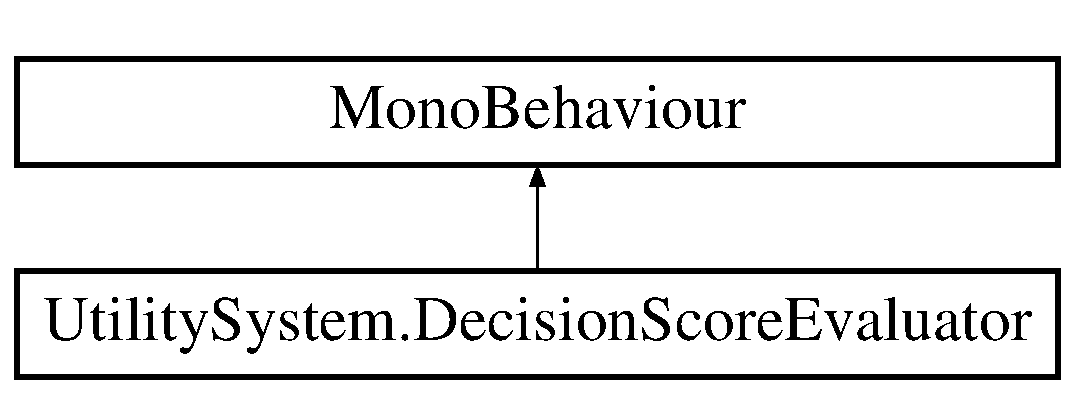
\includegraphics[height=2.000000cm]{class_utility_system_1_1_decision_score_evaluator}
\end{center}
\end{figure}
\subsection*{Public Member Functions}
\begin{DoxyCompactItemize}
\item 
float \mbox{\hyperlink{class_utility_system_1_1_decision_score_evaluator_acf7ab6dfc85d63f780e632430a3cc991}{Score}} (\mbox{\hyperlink{class_utility_system_1_1_decision_context}{Decision\+Context}} context, float bonus, float min)
\end{DoxyCompactItemize}
\subsection*{Public Attributes}
\begin{DoxyCompactItemize}
\item 
string \mbox{\hyperlink{class_utility_system_1_1_decision_score_evaluator_aba9d231541a9c40addd46c83fccdd96b}{description}}
\item 
float \mbox{\hyperlink{class_utility_system_1_1_decision_score_evaluator_a606aa4ec017c2c0aa7e21cdcb8586f34}{weight}}
\item 
\mbox{\hyperlink{class_utility_system_1_1_consideration}{Consideration}} \mbox{[}$\,$\mbox{]} \mbox{\hyperlink{class_utility_system_1_1_decision_score_evaluator_a25c6bcf192097790a27891e542d7beb7}{considerations}}
\end{DoxyCompactItemize}
\subsection*{Protected Member Functions}
\begin{DoxyCompactItemize}
\item 
float \mbox{\hyperlink{class_utility_system_1_1_decision_score_evaluator_aefe0da6966b6e9fa0fad36de6c70add7}{Compensate}} (float original\+Score)
\end{DoxyCompactItemize}


\subsection{Member Function Documentation}
\mbox{\Hypertarget{class_utility_system_1_1_decision_score_evaluator_aefe0da6966b6e9fa0fad36de6c70add7}\label{class_utility_system_1_1_decision_score_evaluator_aefe0da6966b6e9fa0fad36de6c70add7}} 
\index{Utility\+System\+::\+Decision\+Score\+Evaluator@{Utility\+System\+::\+Decision\+Score\+Evaluator}!Compensate@{Compensate}}
\index{Compensate@{Compensate}!Utility\+System\+::\+Decision\+Score\+Evaluator@{Utility\+System\+::\+Decision\+Score\+Evaluator}}
\subsubsection{\texorpdfstring{Compensate()}{Compensate()}}
{\footnotesize\ttfamily float Utility\+System.\+Decision\+Score\+Evaluator.\+Compensate (\begin{DoxyParamCaption}\item[{float}]{original\+Score }\end{DoxyParamCaption})\hspace{0.3cm}{\ttfamily [protected]}}

\mbox{\Hypertarget{class_utility_system_1_1_decision_score_evaluator_acf7ab6dfc85d63f780e632430a3cc991}\label{class_utility_system_1_1_decision_score_evaluator_acf7ab6dfc85d63f780e632430a3cc991}} 
\index{Utility\+System\+::\+Decision\+Score\+Evaluator@{Utility\+System\+::\+Decision\+Score\+Evaluator}!Score@{Score}}
\index{Score@{Score}!Utility\+System\+::\+Decision\+Score\+Evaluator@{Utility\+System\+::\+Decision\+Score\+Evaluator}}
\subsubsection{\texorpdfstring{Score()}{Score()}}
{\footnotesize\ttfamily float Utility\+System.\+Decision\+Score\+Evaluator.\+Score (\begin{DoxyParamCaption}\item[{\mbox{\hyperlink{class_utility_system_1_1_decision_context}{Decision\+Context}}}]{context,  }\item[{float}]{bonus,  }\item[{float}]{min }\end{DoxyParamCaption})}



\subsection{Member Data Documentation}
\mbox{\Hypertarget{class_utility_system_1_1_decision_score_evaluator_a25c6bcf192097790a27891e542d7beb7}\label{class_utility_system_1_1_decision_score_evaluator_a25c6bcf192097790a27891e542d7beb7}} 
\index{Utility\+System\+::\+Decision\+Score\+Evaluator@{Utility\+System\+::\+Decision\+Score\+Evaluator}!considerations@{considerations}}
\index{considerations@{considerations}!Utility\+System\+::\+Decision\+Score\+Evaluator@{Utility\+System\+::\+Decision\+Score\+Evaluator}}
\subsubsection{\texorpdfstring{considerations}{considerations}}
{\footnotesize\ttfamily \mbox{\hyperlink{class_utility_system_1_1_consideration}{Consideration}} \mbox{[}$\,$\mbox{]} Utility\+System.\+Decision\+Score\+Evaluator.\+considerations}

\mbox{\Hypertarget{class_utility_system_1_1_decision_score_evaluator_aba9d231541a9c40addd46c83fccdd96b}\label{class_utility_system_1_1_decision_score_evaluator_aba9d231541a9c40addd46c83fccdd96b}} 
\index{Utility\+System\+::\+Decision\+Score\+Evaluator@{Utility\+System\+::\+Decision\+Score\+Evaluator}!description@{description}}
\index{description@{description}!Utility\+System\+::\+Decision\+Score\+Evaluator@{Utility\+System\+::\+Decision\+Score\+Evaluator}}
\subsubsection{\texorpdfstring{description}{description}}
{\footnotesize\ttfamily string Utility\+System.\+Decision\+Score\+Evaluator.\+description}

\mbox{\Hypertarget{class_utility_system_1_1_decision_score_evaluator_a606aa4ec017c2c0aa7e21cdcb8586f34}\label{class_utility_system_1_1_decision_score_evaluator_a606aa4ec017c2c0aa7e21cdcb8586f34}} 
\index{Utility\+System\+::\+Decision\+Score\+Evaluator@{Utility\+System\+::\+Decision\+Score\+Evaluator}!weight@{weight}}
\index{weight@{weight}!Utility\+System\+::\+Decision\+Score\+Evaluator@{Utility\+System\+::\+Decision\+Score\+Evaluator}}
\subsubsection{\texorpdfstring{weight}{weight}}
{\footnotesize\ttfamily float Utility\+System.\+Decision\+Score\+Evaluator.\+weight}



The documentation for this class was generated from the following file\+:\begin{DoxyCompactItemize}
\item 
/\+Users/sabienambrose/\+Documents/\+Coding/\+Unity\+Mechanical\+Turk/\+Mechanical\+Turk/\+Assets/\+Scripts/\+Framework/\+Utility/\mbox{\hyperlink{_decision_score_evaluator_8cs}{Decision\+Score\+Evaluator.\+cs}}\end{DoxyCompactItemize}

\hypertarget{struct_delaunay_triangle}{}\section{Delaunay\+Triangle Struct Reference}
\label{struct_delaunay_triangle}\index{Delaunay\+Triangle@{Delaunay\+Triangle}}
\subsection*{Public Member Functions}
\begin{DoxyCompactItemize}
\item 
\mbox{\hyperlink{struct_delaunay_triangle_a3346e0ff1d4d37b31293359750e28548}{Delaunay\+Triangle}} (int A, int B, int C)
\item 
\mbox{\hyperlink{struct_delaunay_triangle_a98d84cc9db0152ca7bd5e7181a54382e}{Delaunay\+Triangle}} (\mbox{\hyperlink{struct_int_triangle}{Int\+Triangle}} Tri)
\item 
void \mbox{\hyperlink{struct_delaunay_triangle_aa47e1ddfbb465eb5b0f7de2a356b2ae1}{Add\+Child}} (\mbox{\hyperlink{struct_delaunay_triangle}{Delaunay\+Triangle}} dt)
\item 
void \mbox{\hyperlink{struct_delaunay_triangle_ae8eabb4164875b524a4d826a829bcb05}{Remove\+Child}} (\mbox{\hyperlink{struct_delaunay_triangle}{Delaunay\+Triangle}} dt)
\item 
List$<$ \mbox{\hyperlink{struct_delaunay_triangle}{Delaunay\+Triangle}} $>$ \mbox{\hyperlink{struct_delaunay_triangle_a380da11f8b29fd534ea8ce959364f7f7}{Get\+Triangles}} ()
\item 
\mbox{\hyperlink{struct_int_point}{Int\+Point}} \mbox{[}$\,$\mbox{]} \mbox{\hyperlink{struct_delaunay_triangle_af41ef86382b370cdacbb76fff23b3f6d}{Edges}} ()
\item 
\mbox{\hyperlink{struct_int_point}{Int\+Point}} \mbox{[}$\,$\mbox{]} \mbox{\hyperlink{struct_delaunay_triangle_abfa19827eec8c68badc78c4a9b76e21f}{All\+Edges}} ()
\item 
bool \mbox{\hyperlink{struct_delaunay_triangle_a0b4b4356bd164b7b209074203cf9d666}{Shares\+Vertex\+With}} (\mbox{\hyperlink{struct_delaunay_triangle}{Delaunay\+Triangle}} other)
\item 
bool \mbox{\hyperlink{struct_delaunay_triangle_a5797e4a4cf0ec654433e2d61e5540058}{Has\+Vertex}} (int a)
\item 
bool \mbox{\hyperlink{struct_delaunay_triangle_a5faf014731e3078f4989f56f46ce2845}{Has\+Edge}} (\mbox{\hyperlink{struct_int_point}{Int\+Point}} edge)
\item 
bool \mbox{\hyperlink{struct_delaunay_triangle_afbf1696692f10be76c4d701aa2c918f0}{Has\+Edge}} (int a, int b)
\item 
override bool \mbox{\hyperlink{struct_delaunay_triangle_a32169a31c41b6f4f2a223a7dfdbf4b08}{Equals}} (object obj)
\end{DoxyCompactItemize}
\subsection*{Public Attributes}
\begin{DoxyCompactItemize}
\item 
\mbox{\hyperlink{struct_int_triangle}{Int\+Triangle}} \mbox{\hyperlink{struct_delaunay_triangle_ade0daceebe739c61341e33e5dddb2efc}{Triangle}}
\end{DoxyCompactItemize}


\subsection{Constructor \& Destructor Documentation}
\mbox{\Hypertarget{struct_delaunay_triangle_a3346e0ff1d4d37b31293359750e28548}\label{struct_delaunay_triangle_a3346e0ff1d4d37b31293359750e28548}} 
\index{Delaunay\+Triangle@{Delaunay\+Triangle}!Delaunay\+Triangle@{Delaunay\+Triangle}}
\index{Delaunay\+Triangle@{Delaunay\+Triangle}!Delaunay\+Triangle@{Delaunay\+Triangle}}
\subsubsection{\texorpdfstring{Delaunay\+Triangle()}{DelaunayTriangle()}\hspace{0.1cm}{\footnotesize\ttfamily [1/2]}}
{\footnotesize\ttfamily Delaunay\+Triangle.\+Delaunay\+Triangle (\begin{DoxyParamCaption}\item[{int}]{A,  }\item[{int}]{B,  }\item[{int}]{C }\end{DoxyParamCaption})}

\mbox{\Hypertarget{struct_delaunay_triangle_a98d84cc9db0152ca7bd5e7181a54382e}\label{struct_delaunay_triangle_a98d84cc9db0152ca7bd5e7181a54382e}} 
\index{Delaunay\+Triangle@{Delaunay\+Triangle}!Delaunay\+Triangle@{Delaunay\+Triangle}}
\index{Delaunay\+Triangle@{Delaunay\+Triangle}!Delaunay\+Triangle@{Delaunay\+Triangle}}
\subsubsection{\texorpdfstring{Delaunay\+Triangle()}{DelaunayTriangle()}\hspace{0.1cm}{\footnotesize\ttfamily [2/2]}}
{\footnotesize\ttfamily Delaunay\+Triangle.\+Delaunay\+Triangle (\begin{DoxyParamCaption}\item[{\mbox{\hyperlink{struct_int_triangle}{Int\+Triangle}}}]{Tri }\end{DoxyParamCaption})}



\subsection{Member Function Documentation}
\mbox{\Hypertarget{struct_delaunay_triangle_aa47e1ddfbb465eb5b0f7de2a356b2ae1}\label{struct_delaunay_triangle_aa47e1ddfbb465eb5b0f7de2a356b2ae1}} 
\index{Delaunay\+Triangle@{Delaunay\+Triangle}!Add\+Child@{Add\+Child}}
\index{Add\+Child@{Add\+Child}!Delaunay\+Triangle@{Delaunay\+Triangle}}
\subsubsection{\texorpdfstring{Add\+Child()}{AddChild()}}
{\footnotesize\ttfamily void Delaunay\+Triangle.\+Add\+Child (\begin{DoxyParamCaption}\item[{\mbox{\hyperlink{struct_delaunay_triangle}{Delaunay\+Triangle}}}]{dt }\end{DoxyParamCaption})}

\mbox{\Hypertarget{struct_delaunay_triangle_abfa19827eec8c68badc78c4a9b76e21f}\label{struct_delaunay_triangle_abfa19827eec8c68badc78c4a9b76e21f}} 
\index{Delaunay\+Triangle@{Delaunay\+Triangle}!All\+Edges@{All\+Edges}}
\index{All\+Edges@{All\+Edges}!Delaunay\+Triangle@{Delaunay\+Triangle}}
\subsubsection{\texorpdfstring{All\+Edges()}{AllEdges()}}
{\footnotesize\ttfamily \mbox{\hyperlink{struct_int_point}{Int\+Point}} \mbox{[}$\,$\mbox{]} Delaunay\+Triangle.\+All\+Edges (\begin{DoxyParamCaption}{ }\end{DoxyParamCaption})}

\mbox{\Hypertarget{struct_delaunay_triangle_af41ef86382b370cdacbb76fff23b3f6d}\label{struct_delaunay_triangle_af41ef86382b370cdacbb76fff23b3f6d}} 
\index{Delaunay\+Triangle@{Delaunay\+Triangle}!Edges@{Edges}}
\index{Edges@{Edges}!Delaunay\+Triangle@{Delaunay\+Triangle}}
\subsubsection{\texorpdfstring{Edges()}{Edges()}}
{\footnotesize\ttfamily \mbox{\hyperlink{struct_int_point}{Int\+Point}} \mbox{[}$\,$\mbox{]} Delaunay\+Triangle.\+Edges (\begin{DoxyParamCaption}{ }\end{DoxyParamCaption})}

\mbox{\Hypertarget{struct_delaunay_triangle_a32169a31c41b6f4f2a223a7dfdbf4b08}\label{struct_delaunay_triangle_a32169a31c41b6f4f2a223a7dfdbf4b08}} 
\index{Delaunay\+Triangle@{Delaunay\+Triangle}!Equals@{Equals}}
\index{Equals@{Equals}!Delaunay\+Triangle@{Delaunay\+Triangle}}
\subsubsection{\texorpdfstring{Equals()}{Equals()}}
{\footnotesize\ttfamily override bool Delaunay\+Triangle.\+Equals (\begin{DoxyParamCaption}\item[{object}]{obj }\end{DoxyParamCaption})}

\mbox{\Hypertarget{struct_delaunay_triangle_a380da11f8b29fd534ea8ce959364f7f7}\label{struct_delaunay_triangle_a380da11f8b29fd534ea8ce959364f7f7}} 
\index{Delaunay\+Triangle@{Delaunay\+Triangle}!Get\+Triangles@{Get\+Triangles}}
\index{Get\+Triangles@{Get\+Triangles}!Delaunay\+Triangle@{Delaunay\+Triangle}}
\subsubsection{\texorpdfstring{Get\+Triangles()}{GetTriangles()}}
{\footnotesize\ttfamily List$<$\mbox{\hyperlink{struct_delaunay_triangle}{Delaunay\+Triangle}}$>$ Delaunay\+Triangle.\+Get\+Triangles (\begin{DoxyParamCaption}{ }\end{DoxyParamCaption})}

\mbox{\Hypertarget{struct_delaunay_triangle_a5faf014731e3078f4989f56f46ce2845}\label{struct_delaunay_triangle_a5faf014731e3078f4989f56f46ce2845}} 
\index{Delaunay\+Triangle@{Delaunay\+Triangle}!Has\+Edge@{Has\+Edge}}
\index{Has\+Edge@{Has\+Edge}!Delaunay\+Triangle@{Delaunay\+Triangle}}
\subsubsection{\texorpdfstring{Has\+Edge()}{HasEdge()}\hspace{0.1cm}{\footnotesize\ttfamily [1/2]}}
{\footnotesize\ttfamily bool Delaunay\+Triangle.\+Has\+Edge (\begin{DoxyParamCaption}\item[{\mbox{\hyperlink{struct_int_point}{Int\+Point}}}]{edge }\end{DoxyParamCaption})}

\mbox{\Hypertarget{struct_delaunay_triangle_afbf1696692f10be76c4d701aa2c918f0}\label{struct_delaunay_triangle_afbf1696692f10be76c4d701aa2c918f0}} 
\index{Delaunay\+Triangle@{Delaunay\+Triangle}!Has\+Edge@{Has\+Edge}}
\index{Has\+Edge@{Has\+Edge}!Delaunay\+Triangle@{Delaunay\+Triangle}}
\subsubsection{\texorpdfstring{Has\+Edge()}{HasEdge()}\hspace{0.1cm}{\footnotesize\ttfamily [2/2]}}
{\footnotesize\ttfamily bool Delaunay\+Triangle.\+Has\+Edge (\begin{DoxyParamCaption}\item[{int}]{a,  }\item[{int}]{b }\end{DoxyParamCaption})}

\mbox{\Hypertarget{struct_delaunay_triangle_a5797e4a4cf0ec654433e2d61e5540058}\label{struct_delaunay_triangle_a5797e4a4cf0ec654433e2d61e5540058}} 
\index{Delaunay\+Triangle@{Delaunay\+Triangle}!Has\+Vertex@{Has\+Vertex}}
\index{Has\+Vertex@{Has\+Vertex}!Delaunay\+Triangle@{Delaunay\+Triangle}}
\subsubsection{\texorpdfstring{Has\+Vertex()}{HasVertex()}}
{\footnotesize\ttfamily bool Delaunay\+Triangle.\+Has\+Vertex (\begin{DoxyParamCaption}\item[{int}]{a }\end{DoxyParamCaption})}

\mbox{\Hypertarget{struct_delaunay_triangle_ae8eabb4164875b524a4d826a829bcb05}\label{struct_delaunay_triangle_ae8eabb4164875b524a4d826a829bcb05}} 
\index{Delaunay\+Triangle@{Delaunay\+Triangle}!Remove\+Child@{Remove\+Child}}
\index{Remove\+Child@{Remove\+Child}!Delaunay\+Triangle@{Delaunay\+Triangle}}
\subsubsection{\texorpdfstring{Remove\+Child()}{RemoveChild()}}
{\footnotesize\ttfamily void Delaunay\+Triangle.\+Remove\+Child (\begin{DoxyParamCaption}\item[{\mbox{\hyperlink{struct_delaunay_triangle}{Delaunay\+Triangle}}}]{dt }\end{DoxyParamCaption})}

\mbox{\Hypertarget{struct_delaunay_triangle_a0b4b4356bd164b7b209074203cf9d666}\label{struct_delaunay_triangle_a0b4b4356bd164b7b209074203cf9d666}} 
\index{Delaunay\+Triangle@{Delaunay\+Triangle}!Shares\+Vertex\+With@{Shares\+Vertex\+With}}
\index{Shares\+Vertex\+With@{Shares\+Vertex\+With}!Delaunay\+Triangle@{Delaunay\+Triangle}}
\subsubsection{\texorpdfstring{Shares\+Vertex\+With()}{SharesVertexWith()}}
{\footnotesize\ttfamily bool Delaunay\+Triangle.\+Shares\+Vertex\+With (\begin{DoxyParamCaption}\item[{\mbox{\hyperlink{struct_delaunay_triangle}{Delaunay\+Triangle}}}]{other }\end{DoxyParamCaption})}



\subsection{Member Data Documentation}
\mbox{\Hypertarget{struct_delaunay_triangle_ade0daceebe739c61341e33e5dddb2efc}\label{struct_delaunay_triangle_ade0daceebe739c61341e33e5dddb2efc}} 
\index{Delaunay\+Triangle@{Delaunay\+Triangle}!Triangle@{Triangle}}
\index{Triangle@{Triangle}!Delaunay\+Triangle@{Delaunay\+Triangle}}
\subsubsection{\texorpdfstring{Triangle}{Triangle}}
{\footnotesize\ttfamily \mbox{\hyperlink{struct_int_triangle}{Int\+Triangle}} Delaunay\+Triangle.\+Triangle}



The documentation for this struct was generated from the following file\+:\begin{DoxyCompactItemize}
\item 
/\+Users/sabienambrose/\+Documents/\+Coding/\+Unity\+Mechanical\+Turk/\+Mechanical\+Turk/\+Assets/\+Scripts/\+Util/\+Containers/\+Graphs/\+Triangle\+Graphs/\mbox{\hyperlink{_delaunay_triangulation_8cs}{Delaunay\+Triangulation.\+cs}}\end{DoxyCompactItemize}

\hypertarget{class_delaunay_triangulation}{}\section{Delaunay\+Triangulation Class Reference}
\label{class_delaunay_triangulation}\index{Delaunay\+Triangulation@{Delaunay\+Triangulation}}
Inheritance diagram for Delaunay\+Triangulation\+:\begin{figure}[H]
\begin{center}
\leavevmode
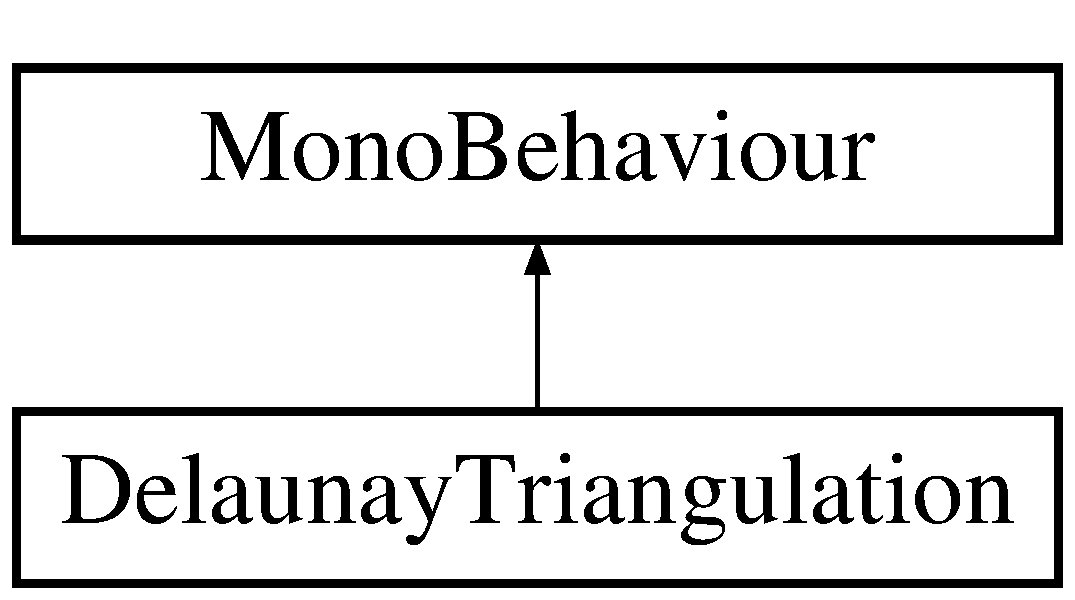
\includegraphics[height=2.000000cm]{class_delaunay_triangulation}
\end{center}
\end{figure}
\subsection*{Public Member Functions}
\begin{DoxyCompactItemize}
\item 
void \mbox{\hyperlink{class_delaunay_triangulation_a0edb936dc23053ec75ffecfb7a426c03}{Init}} ()
\item 
Vector2 \mbox{[}$\,$\mbox{]} \mbox{\hyperlink{class_delaunay_triangulation_a1f871cd0ab4b06003e92c9aa02683f5a}{Corners}} ()
\item 
void \mbox{\hyperlink{class_delaunay_triangulation_a2880d1fc8f58a1c500da8276e31fbddc}{Add\+Point}} (Vector2 New\+Point)
\item 
bool \mbox{\hyperlink{class_delaunay_triangulation_a81fe4e7d4347425f00d973cad4215fc6}{Is\+Point\+Inside\+Circumcircle}} (Vector2 p, \mbox{\hyperlink{struct_delaunay_triangle}{Delaunay\+Triangle}} dt)
\item 
bool \mbox{\hyperlink{class_delaunay_triangulation_a1f1b19add4ee96d9613b47fe19106a94}{Is\+Point\+Inside\+Circumcircle}} (Vector2 p, \mbox{\hyperlink{struct_int_triangle}{Int\+Triangle}} dt)
\item 
Vector2 \mbox{[}$\,$\mbox{]} \mbox{\hyperlink{class_delaunay_triangulation_a44384b9db3229395f862673e9ec03296}{Get\+Points}} ()
\item 
\mbox{\hyperlink{struct_int_point}{Int\+Point}} \mbox{[}$\,$\mbox{]} \mbox{\hyperlink{class_delaunay_triangulation_afcf101ed329a388d5b2c1e720f3cfb41}{Get\+Edges}} ()
\item 
\mbox{\hyperlink{struct_int_triangle}{Int\+Triangle}} \mbox{[}$\,$\mbox{]} \mbox{\hyperlink{class_delaunay_triangulation_a1b55615a70f1a68c150f397be89357bf}{Get\+Triangles}} ()
\item 
void \mbox{\hyperlink{class_delaunay_triangulation_ab740dde5362f8e54c4d000d6cd82d57c}{On\+Draw\+Gizmos\+Selected}} ()
\item 
Color \mbox{\hyperlink{class_delaunay_triangulation_a5c2e4b787760bd7aa248933bce6b97b2}{Get\+Point\+Color}} (Vector2 P)
\end{DoxyCompactItemize}
\subsection*{Public Attributes}
\begin{DoxyCompactItemize}
\item 
Polygon\+Collider2D \mbox{\hyperlink{class_delaunay_triangulation_aeb242e46a6c940c61502ea5e08d4b5b6}{bounds}}
\end{DoxyCompactItemize}
\subsection*{Protected Member Functions}
\begin{DoxyCompactItemize}
\item 
void \mbox{\hyperlink{class_delaunay_triangulation_aa4ae5153592df4ba083d810a6d809999}{Update\+Triangles}} (Vector2 New\+Point)
\item 
void \mbox{\hyperlink{class_delaunay_triangulation_aa4b708614e1c66fde876d036630804da}{Update\+Deltris}} (Vector2 New\+Point)
\end{DoxyCompactItemize}
\subsection*{Protected Attributes}
\begin{DoxyCompactItemize}
\item 
int \mbox{\hyperlink{class_delaunay_triangulation_a04fce817ac5bdbc5ac2891e0efc8626b}{Num\+Triangles}} = 0
\item 
int \mbox{\hyperlink{class_delaunay_triangulation_aecaad9bab22a717e9ec4e91191896d83}{Num\+Points}} = 0
\item 
List$<$ Vector2 $>$ \mbox{\hyperlink{class_delaunay_triangulation_abe36cb50d65f6fa86fa15dba1cb413a5}{points}} = new List$<$Vector2$>$()
\item 
List$<$ \mbox{\hyperlink{struct_int_triangle}{Int\+Triangle}} $>$ \mbox{\hyperlink{class_delaunay_triangulation_a51e3e7d9301274730cba64afc6ce69cb}{triangles}} = new List$<$\mbox{\hyperlink{struct_int_triangle}{Int\+Triangle}}$>$()
\end{DoxyCompactItemize}


\subsection{Member Function Documentation}
\mbox{\Hypertarget{class_delaunay_triangulation_a2880d1fc8f58a1c500da8276e31fbddc}\label{class_delaunay_triangulation_a2880d1fc8f58a1c500da8276e31fbddc}} 
\index{Delaunay\+Triangulation@{Delaunay\+Triangulation}!Add\+Point@{Add\+Point}}
\index{Add\+Point@{Add\+Point}!Delaunay\+Triangulation@{Delaunay\+Triangulation}}
\subsubsection{\texorpdfstring{Add\+Point()}{AddPoint()}}
{\footnotesize\ttfamily void Delaunay\+Triangulation.\+Add\+Point (\begin{DoxyParamCaption}\item[{Vector2}]{New\+Point }\end{DoxyParamCaption})}

~\newline
 for each triangle in triangulation // done inserting points, now clean up if triangle contains a vertex from original super-\/triangle remove triangle from triangulation\mbox{\Hypertarget{class_delaunay_triangulation_a1f871cd0ab4b06003e92c9aa02683f5a}\label{class_delaunay_triangulation_a1f871cd0ab4b06003e92c9aa02683f5a}} 
\index{Delaunay\+Triangulation@{Delaunay\+Triangulation}!Corners@{Corners}}
\index{Corners@{Corners}!Delaunay\+Triangulation@{Delaunay\+Triangulation}}
\subsubsection{\texorpdfstring{Corners()}{Corners()}}
{\footnotesize\ttfamily Vector2 \mbox{[}$\,$\mbox{]} Delaunay\+Triangulation.\+Corners (\begin{DoxyParamCaption}{ }\end{DoxyParamCaption})}

\mbox{\Hypertarget{class_delaunay_triangulation_afcf101ed329a388d5b2c1e720f3cfb41}\label{class_delaunay_triangulation_afcf101ed329a388d5b2c1e720f3cfb41}} 
\index{Delaunay\+Triangulation@{Delaunay\+Triangulation}!Get\+Edges@{Get\+Edges}}
\index{Get\+Edges@{Get\+Edges}!Delaunay\+Triangulation@{Delaunay\+Triangulation}}
\subsubsection{\texorpdfstring{Get\+Edges()}{GetEdges()}}
{\footnotesize\ttfamily \mbox{\hyperlink{struct_int_point}{Int\+Point}} \mbox{[}$\,$\mbox{]} Delaunay\+Triangulation.\+Get\+Edges (\begin{DoxyParamCaption}{ }\end{DoxyParamCaption})}

\mbox{\Hypertarget{class_delaunay_triangulation_a5c2e4b787760bd7aa248933bce6b97b2}\label{class_delaunay_triangulation_a5c2e4b787760bd7aa248933bce6b97b2}} 
\index{Delaunay\+Triangulation@{Delaunay\+Triangulation}!Get\+Point\+Color@{Get\+Point\+Color}}
\index{Get\+Point\+Color@{Get\+Point\+Color}!Delaunay\+Triangulation@{Delaunay\+Triangulation}}
\subsubsection{\texorpdfstring{Get\+Point\+Color()}{GetPointColor()}}
{\footnotesize\ttfamily Color Delaunay\+Triangulation.\+Get\+Point\+Color (\begin{DoxyParamCaption}\item[{Vector2}]{P }\end{DoxyParamCaption})}

\mbox{\Hypertarget{class_delaunay_triangulation_a44384b9db3229395f862673e9ec03296}\label{class_delaunay_triangulation_a44384b9db3229395f862673e9ec03296}} 
\index{Delaunay\+Triangulation@{Delaunay\+Triangulation}!Get\+Points@{Get\+Points}}
\index{Get\+Points@{Get\+Points}!Delaunay\+Triangulation@{Delaunay\+Triangulation}}
\subsubsection{\texorpdfstring{Get\+Points()}{GetPoints()}}
{\footnotesize\ttfamily Vector2 \mbox{[}$\,$\mbox{]} Delaunay\+Triangulation.\+Get\+Points (\begin{DoxyParamCaption}{ }\end{DoxyParamCaption})}

\mbox{\Hypertarget{class_delaunay_triangulation_a1b55615a70f1a68c150f397be89357bf}\label{class_delaunay_triangulation_a1b55615a70f1a68c150f397be89357bf}} 
\index{Delaunay\+Triangulation@{Delaunay\+Triangulation}!Get\+Triangles@{Get\+Triangles}}
\index{Get\+Triangles@{Get\+Triangles}!Delaunay\+Triangulation@{Delaunay\+Triangulation}}
\subsubsection{\texorpdfstring{Get\+Triangles()}{GetTriangles()}}
{\footnotesize\ttfamily \mbox{\hyperlink{struct_int_triangle}{Int\+Triangle}} \mbox{[}$\,$\mbox{]} Delaunay\+Triangulation.\+Get\+Triangles (\begin{DoxyParamCaption}{ }\end{DoxyParamCaption})}

\mbox{\Hypertarget{class_delaunay_triangulation_a0edb936dc23053ec75ffecfb7a426c03}\label{class_delaunay_triangulation_a0edb936dc23053ec75ffecfb7a426c03}} 
\index{Delaunay\+Triangulation@{Delaunay\+Triangulation}!Init@{Init}}
\index{Init@{Init}!Delaunay\+Triangulation@{Delaunay\+Triangulation}}
\subsubsection{\texorpdfstring{Init()}{Init()}}
{\footnotesize\ttfamily void Delaunay\+Triangulation.\+Init (\begin{DoxyParamCaption}{ }\end{DoxyParamCaption})}

\mbox{\Hypertarget{class_delaunay_triangulation_a81fe4e7d4347425f00d973cad4215fc6}\label{class_delaunay_triangulation_a81fe4e7d4347425f00d973cad4215fc6}} 
\index{Delaunay\+Triangulation@{Delaunay\+Triangulation}!Is\+Point\+Inside\+Circumcircle@{Is\+Point\+Inside\+Circumcircle}}
\index{Is\+Point\+Inside\+Circumcircle@{Is\+Point\+Inside\+Circumcircle}!Delaunay\+Triangulation@{Delaunay\+Triangulation}}
\subsubsection{\texorpdfstring{Is\+Point\+Inside\+Circumcircle()}{IsPointInsideCircumcircle()}\hspace{0.1cm}{\footnotesize\ttfamily [1/2]}}
{\footnotesize\ttfamily bool Delaunay\+Triangulation.\+Is\+Point\+Inside\+Circumcircle (\begin{DoxyParamCaption}\item[{Vector2}]{p,  }\item[{\mbox{\hyperlink{struct_delaunay_triangle}{Delaunay\+Triangle}}}]{dt }\end{DoxyParamCaption})}

\mbox{\Hypertarget{class_delaunay_triangulation_a1f1b19add4ee96d9613b47fe19106a94}\label{class_delaunay_triangulation_a1f1b19add4ee96d9613b47fe19106a94}} 
\index{Delaunay\+Triangulation@{Delaunay\+Triangulation}!Is\+Point\+Inside\+Circumcircle@{Is\+Point\+Inside\+Circumcircle}}
\index{Is\+Point\+Inside\+Circumcircle@{Is\+Point\+Inside\+Circumcircle}!Delaunay\+Triangulation@{Delaunay\+Triangulation}}
\subsubsection{\texorpdfstring{Is\+Point\+Inside\+Circumcircle()}{IsPointInsideCircumcircle()}\hspace{0.1cm}{\footnotesize\ttfamily [2/2]}}
{\footnotesize\ttfamily bool Delaunay\+Triangulation.\+Is\+Point\+Inside\+Circumcircle (\begin{DoxyParamCaption}\item[{Vector2}]{p,  }\item[{\mbox{\hyperlink{struct_int_triangle}{Int\+Triangle}}}]{dt }\end{DoxyParamCaption})}

\mbox{\Hypertarget{class_delaunay_triangulation_ab740dde5362f8e54c4d000d6cd82d57c}\label{class_delaunay_triangulation_ab740dde5362f8e54c4d000d6cd82d57c}} 
\index{Delaunay\+Triangulation@{Delaunay\+Triangulation}!On\+Draw\+Gizmos\+Selected@{On\+Draw\+Gizmos\+Selected}}
\index{On\+Draw\+Gizmos\+Selected@{On\+Draw\+Gizmos\+Selected}!Delaunay\+Triangulation@{Delaunay\+Triangulation}}
\subsubsection{\texorpdfstring{On\+Draw\+Gizmos\+Selected()}{OnDrawGizmosSelected()}}
{\footnotesize\ttfamily void Delaunay\+Triangulation.\+On\+Draw\+Gizmos\+Selected (\begin{DoxyParamCaption}{ }\end{DoxyParamCaption})}

\mbox{\Hypertarget{class_delaunay_triangulation_aa4b708614e1c66fde876d036630804da}\label{class_delaunay_triangulation_aa4b708614e1c66fde876d036630804da}} 
\index{Delaunay\+Triangulation@{Delaunay\+Triangulation}!Update\+Deltris@{Update\+Deltris}}
\index{Update\+Deltris@{Update\+Deltris}!Delaunay\+Triangulation@{Delaunay\+Triangulation}}
\subsubsection{\texorpdfstring{Update\+Deltris()}{UpdateDeltris()}}
{\footnotesize\ttfamily void Delaunay\+Triangulation.\+Update\+Deltris (\begin{DoxyParamCaption}\item[{Vector2}]{New\+Point }\end{DoxyParamCaption})\hspace{0.3cm}{\ttfamily [protected]}}

\mbox{\Hypertarget{class_delaunay_triangulation_aa4ae5153592df4ba083d810a6d809999}\label{class_delaunay_triangulation_aa4ae5153592df4ba083d810a6d809999}} 
\index{Delaunay\+Triangulation@{Delaunay\+Triangulation}!Update\+Triangles@{Update\+Triangles}}
\index{Update\+Triangles@{Update\+Triangles}!Delaunay\+Triangulation@{Delaunay\+Triangulation}}
\subsubsection{\texorpdfstring{Update\+Triangles()}{UpdateTriangles()}}
{\footnotesize\ttfamily void Delaunay\+Triangulation.\+Update\+Triangles (\begin{DoxyParamCaption}\item[{Vector2}]{New\+Point }\end{DoxyParamCaption})\hspace{0.3cm}{\ttfamily [protected]}}

~\newline
 for each triangle in triangulation // done inserting points, now clean up if triangle contains a vertex from original super-\/triangle remove triangle from triangulation

\subsection{Member Data Documentation}
\mbox{\Hypertarget{class_delaunay_triangulation_aeb242e46a6c940c61502ea5e08d4b5b6}\label{class_delaunay_triangulation_aeb242e46a6c940c61502ea5e08d4b5b6}} 
\index{Delaunay\+Triangulation@{Delaunay\+Triangulation}!bounds@{bounds}}
\index{bounds@{bounds}!Delaunay\+Triangulation@{Delaunay\+Triangulation}}
\subsubsection{\texorpdfstring{bounds}{bounds}}
{\footnotesize\ttfamily Polygon\+Collider2D Delaunay\+Triangulation.\+bounds}

\mbox{\Hypertarget{class_delaunay_triangulation_aecaad9bab22a717e9ec4e91191896d83}\label{class_delaunay_triangulation_aecaad9bab22a717e9ec4e91191896d83}} 
\index{Delaunay\+Triangulation@{Delaunay\+Triangulation}!Num\+Points@{Num\+Points}}
\index{Num\+Points@{Num\+Points}!Delaunay\+Triangulation@{Delaunay\+Triangulation}}
\subsubsection{\texorpdfstring{Num\+Points}{NumPoints}}
{\footnotesize\ttfamily int Delaunay\+Triangulation.\+Num\+Points = 0\hspace{0.3cm}{\ttfamily [protected]}}

\mbox{\Hypertarget{class_delaunay_triangulation_a04fce817ac5bdbc5ac2891e0efc8626b}\label{class_delaunay_triangulation_a04fce817ac5bdbc5ac2891e0efc8626b}} 
\index{Delaunay\+Triangulation@{Delaunay\+Triangulation}!Num\+Triangles@{Num\+Triangles}}
\index{Num\+Triangles@{Num\+Triangles}!Delaunay\+Triangulation@{Delaunay\+Triangulation}}
\subsubsection{\texorpdfstring{Num\+Triangles}{NumTriangles}}
{\footnotesize\ttfamily int Delaunay\+Triangulation.\+Num\+Triangles = 0\hspace{0.3cm}{\ttfamily [protected]}}

\mbox{\Hypertarget{class_delaunay_triangulation_abe36cb50d65f6fa86fa15dba1cb413a5}\label{class_delaunay_triangulation_abe36cb50d65f6fa86fa15dba1cb413a5}} 
\index{Delaunay\+Triangulation@{Delaunay\+Triangulation}!points@{points}}
\index{points@{points}!Delaunay\+Triangulation@{Delaunay\+Triangulation}}
\subsubsection{\texorpdfstring{points}{points}}
{\footnotesize\ttfamily List$<$Vector2$>$ Delaunay\+Triangulation.\+points = new List$<$Vector2$>$()\hspace{0.3cm}{\ttfamily [protected]}}

\mbox{\Hypertarget{class_delaunay_triangulation_a51e3e7d9301274730cba64afc6ce69cb}\label{class_delaunay_triangulation_a51e3e7d9301274730cba64afc6ce69cb}} 
\index{Delaunay\+Triangulation@{Delaunay\+Triangulation}!triangles@{triangles}}
\index{triangles@{triangles}!Delaunay\+Triangulation@{Delaunay\+Triangulation}}
\subsubsection{\texorpdfstring{triangles}{triangles}}
{\footnotesize\ttfamily List$<$\mbox{\hyperlink{struct_int_triangle}{Int\+Triangle}}$>$ Delaunay\+Triangulation.\+triangles = new List$<$\mbox{\hyperlink{struct_int_triangle}{Int\+Triangle}}$>$()\hspace{0.3cm}{\ttfamily [protected]}}



The documentation for this class was generated from the following file\+:\begin{DoxyCompactItemize}
\item 
/\+Users/sabienambrose/\+Documents/\+Coding/\+Unity\+Mechanical\+Turk/\+Mechanical\+Turk/\+Assets/\+Scripts/\+Util/\+Containers/\+Graphs/\+Triangle\+Graphs/\mbox{\hyperlink{_delaunay_triangulation_8cs}{Delaunay\+Triangulation.\+cs}}\end{DoxyCompactItemize}

\hypertarget{class_euclidean_heuristic}{}\section{Euclidean\+Heuristic Class Reference}
\label{class_euclidean_heuristic}\index{Euclidean\+Heuristic@{Euclidean\+Heuristic}}
Inheritance diagram for Euclidean\+Heuristic\+:\begin{figure}[H]
\begin{center}
\leavevmode
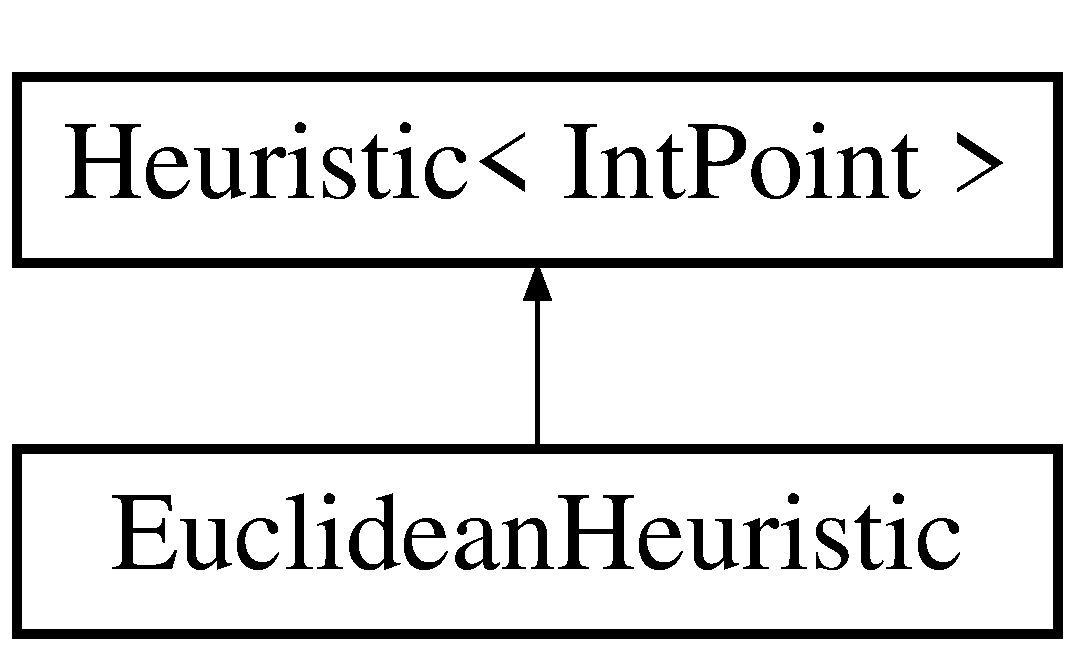
\includegraphics[height=2.000000cm]{class_euclidean_heuristic}
\end{center}
\end{figure}
\subsection*{Public Member Functions}
\begin{DoxyCompactItemize}
\item 
\mbox{\hyperlink{class_euclidean_heuristic_a19c7f55760595e58adfb0cbf5c1e15b8}{Euclidean\+Heuristic}} (\mbox{\hyperlink{struct_int_point}{Int\+Point}} \mbox{\hyperlink{class_heuristic_a9b7078c615bf30ac77f026a737d6169a}{goal}})
\item 
override float \mbox{\hyperlink{class_euclidean_heuristic_a99dffc6647fe187d9b24f64c71f4e6a3}{Estimate}} (\mbox{\hyperlink{struct_int_point}{Int\+Point}} node)
\begin{DoxyCompactList}\small\item\em Returns Euclidean distance between given node and goal node. \end{DoxyCompactList}\end{DoxyCompactItemize}
\subsection*{Additional Inherited Members}


\subsection{Constructor \& Destructor Documentation}
\mbox{\Hypertarget{class_euclidean_heuristic_a19c7f55760595e58adfb0cbf5c1e15b8}\label{class_euclidean_heuristic_a19c7f55760595e58adfb0cbf5c1e15b8}} 
\index{Euclidean\+Heuristic@{Euclidean\+Heuristic}!Euclidean\+Heuristic@{Euclidean\+Heuristic}}
\index{Euclidean\+Heuristic@{Euclidean\+Heuristic}!Euclidean\+Heuristic@{Euclidean\+Heuristic}}
\subsubsection{\texorpdfstring{Euclidean\+Heuristic()}{EuclideanHeuristic()}}
{\footnotesize\ttfamily Euclidean\+Heuristic.\+Euclidean\+Heuristic (\begin{DoxyParamCaption}\item[{\mbox{\hyperlink{struct_int_point}{Int\+Point}}}]{goal }\end{DoxyParamCaption})}



\subsection{Member Function Documentation}
\mbox{\Hypertarget{class_euclidean_heuristic_a99dffc6647fe187d9b24f64c71f4e6a3}\label{class_euclidean_heuristic_a99dffc6647fe187d9b24f64c71f4e6a3}} 
\index{Euclidean\+Heuristic@{Euclidean\+Heuristic}!Estimate@{Estimate}}
\index{Estimate@{Estimate}!Euclidean\+Heuristic@{Euclidean\+Heuristic}}
\subsubsection{\texorpdfstring{Estimate()}{Estimate()}}
{\footnotesize\ttfamily override float Euclidean\+Heuristic.\+Estimate (\begin{DoxyParamCaption}\item[{\mbox{\hyperlink{struct_int_point}{Int\+Point}}}]{node }\end{DoxyParamCaption})}



Returns Euclidean distance between given node and goal node. 


\begin{DoxyParams}{Parameters}
{\em node} & \\
\hline
\end{DoxyParams}
\begin{DoxyReturn}{Returns}

\end{DoxyReturn}


The documentation for this class was generated from the following file\+:\begin{DoxyCompactItemize}
\item 
/\+Users/sabienambrose/\+Documents/\+Coding/\+Unity\+Mechanical\+Turk/\+Mechanical\+Turk/\+Assets/\+Scripts/\+Pathfinding/\+Heuristics/\mbox{\hyperlink{_euclidean_heuristic_8cs}{Euclidean\+Heuristic.\+cs}}\end{DoxyCompactItemize}

\hypertarget{class_game_node}{}\section{Game\+Node Class Reference}
\label{class_game_node}\index{Game\+Node@{Game\+Node}}
Inheritance diagram for Game\+Node\+:\begin{figure}[H]
\begin{center}
\leavevmode
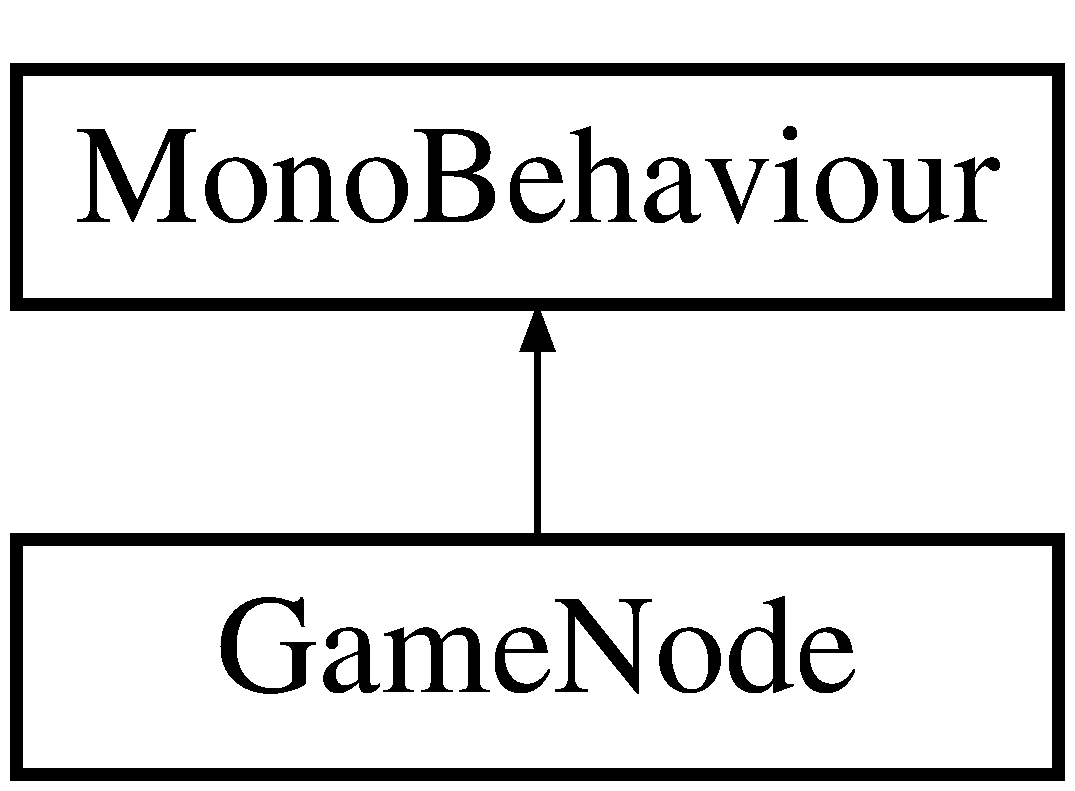
\includegraphics[height=2.000000cm]{class_game_node}
\end{center}
\end{figure}
\subsection*{Public Member Functions}
\begin{DoxyCompactItemize}
\item 
void \mbox{\hyperlink{class_game_node_ac4c8f9eaeeb02827025d4999f461e4f7}{Set\+Node}} (\mbox{\hyperlink{class_node}{Node}} \mbox{\hyperlink{class_game_node_a1358112884b99c36b3a37c4e65c24529}{node}})
\item 
void \mbox{\hyperlink{class_game_node_a28d8bb98f35b26d076a02f656708c798}{Spawn\+Buildings}} ()
\item 
Game\+Object \mbox{\hyperlink{class_game_node_a7769f0664b29bd4ce2178f5c3d511acc}{Get\+Random\+Prefab}} ()
\end{DoxyCompactItemize}
\subsection*{Public Attributes}
\begin{DoxyCompactItemize}
\item 
Game\+Object \mbox{[}$\,$\mbox{]} \mbox{\hyperlink{class_game_node_a7ef395d481491d0bced8c3be6fc62e85}{prefab\+Options}}
\item 
Vector3 \mbox{\hyperlink{class_game_node_a77a1bb6b3f3feaf660ae439ffd2eb416}{spawn\+Space}} = new Vector3(25, 0, 25)
\item 
Vector3 \mbox{\hyperlink{class_game_node_aa7c6a7c1b7d5142f202677b6346078e2}{min\+Location}} = new Vector3(-\/50,0, 50)
\item 
Vector3 \mbox{\hyperlink{class_game_node_a7c5ba008814c712e85e9fea00ab1e29b}{max\+Location}} = new Vector3(-\/50,0, 50)
\end{DoxyCompactItemize}
\subsection*{Protected Attributes}
\begin{DoxyCompactItemize}
\item 
\mbox{\hyperlink{class_node}{Node}} \mbox{\hyperlink{class_game_node_a1358112884b99c36b3a37c4e65c24529}{node}}
\end{DoxyCompactItemize}


\subsection{Member Function Documentation}
\mbox{\Hypertarget{class_game_node_a7769f0664b29bd4ce2178f5c3d511acc}\label{class_game_node_a7769f0664b29bd4ce2178f5c3d511acc}} 
\index{Game\+Node@{Game\+Node}!Get\+Random\+Prefab@{Get\+Random\+Prefab}}
\index{Get\+Random\+Prefab@{Get\+Random\+Prefab}!Game\+Node@{Game\+Node}}
\subsubsection{\texorpdfstring{Get\+Random\+Prefab()}{GetRandomPrefab()}}
{\footnotesize\ttfamily Game\+Object Game\+Node.\+Get\+Random\+Prefab (\begin{DoxyParamCaption}{ }\end{DoxyParamCaption})}

\mbox{\Hypertarget{class_game_node_ac4c8f9eaeeb02827025d4999f461e4f7}\label{class_game_node_ac4c8f9eaeeb02827025d4999f461e4f7}} 
\index{Game\+Node@{Game\+Node}!Set\+Node@{Set\+Node}}
\index{Set\+Node@{Set\+Node}!Game\+Node@{Game\+Node}}
\subsubsection{\texorpdfstring{Set\+Node()}{SetNode()}}
{\footnotesize\ttfamily void Game\+Node.\+Set\+Node (\begin{DoxyParamCaption}\item[{\mbox{\hyperlink{class_node}{Node}}}]{node }\end{DoxyParamCaption})}

\mbox{\Hypertarget{class_game_node_a28d8bb98f35b26d076a02f656708c798}\label{class_game_node_a28d8bb98f35b26d076a02f656708c798}} 
\index{Game\+Node@{Game\+Node}!Spawn\+Buildings@{Spawn\+Buildings}}
\index{Spawn\+Buildings@{Spawn\+Buildings}!Game\+Node@{Game\+Node}}
\subsubsection{\texorpdfstring{Spawn\+Buildings()}{SpawnBuildings()}}
{\footnotesize\ttfamily void Game\+Node.\+Spawn\+Buildings (\begin{DoxyParamCaption}{ }\end{DoxyParamCaption})}



\subsection{Member Data Documentation}
\mbox{\Hypertarget{class_game_node_a7c5ba008814c712e85e9fea00ab1e29b}\label{class_game_node_a7c5ba008814c712e85e9fea00ab1e29b}} 
\index{Game\+Node@{Game\+Node}!max\+Location@{max\+Location}}
\index{max\+Location@{max\+Location}!Game\+Node@{Game\+Node}}
\subsubsection{\texorpdfstring{max\+Location}{maxLocation}}
{\footnotesize\ttfamily Vector3 Game\+Node.\+max\+Location = new Vector3(-\/50,0, 50)}

\mbox{\Hypertarget{class_game_node_aa7c6a7c1b7d5142f202677b6346078e2}\label{class_game_node_aa7c6a7c1b7d5142f202677b6346078e2}} 
\index{Game\+Node@{Game\+Node}!min\+Location@{min\+Location}}
\index{min\+Location@{min\+Location}!Game\+Node@{Game\+Node}}
\subsubsection{\texorpdfstring{min\+Location}{minLocation}}
{\footnotesize\ttfamily Vector3 Game\+Node.\+min\+Location = new Vector3(-\/50,0, 50)}

\mbox{\Hypertarget{class_game_node_a1358112884b99c36b3a37c4e65c24529}\label{class_game_node_a1358112884b99c36b3a37c4e65c24529}} 
\index{Game\+Node@{Game\+Node}!node@{node}}
\index{node@{node}!Game\+Node@{Game\+Node}}
\subsubsection{\texorpdfstring{node}{node}}
{\footnotesize\ttfamily \mbox{\hyperlink{class_node}{Node}} Game\+Node.\+node\hspace{0.3cm}{\ttfamily [protected]}}

\mbox{\Hypertarget{class_game_node_a7ef395d481491d0bced8c3be6fc62e85}\label{class_game_node_a7ef395d481491d0bced8c3be6fc62e85}} 
\index{Game\+Node@{Game\+Node}!prefab\+Options@{prefab\+Options}}
\index{prefab\+Options@{prefab\+Options}!Game\+Node@{Game\+Node}}
\subsubsection{\texorpdfstring{prefab\+Options}{prefabOptions}}
{\footnotesize\ttfamily Game\+Object \mbox{[}$\,$\mbox{]} Game\+Node.\+prefab\+Options}

\mbox{\Hypertarget{class_game_node_a77a1bb6b3f3feaf660ae439ffd2eb416}\label{class_game_node_a77a1bb6b3f3feaf660ae439ffd2eb416}} 
\index{Game\+Node@{Game\+Node}!spawn\+Space@{spawn\+Space}}
\index{spawn\+Space@{spawn\+Space}!Game\+Node@{Game\+Node}}
\subsubsection{\texorpdfstring{spawn\+Space}{spawnSpace}}
{\footnotesize\ttfamily Vector3 Game\+Node.\+spawn\+Space = new Vector3(25, 0, 25)}



The documentation for this class was generated from the following file\+:\begin{DoxyCompactItemize}
\item 
/\+Users/sabienambrose/\+Documents/\+Coding/\+Unity\+Mechanical\+Turk/\+Mechanical\+Turk/\+Assets/\+Scripts/\+Util/\+Containers/\+Graphs/\+Grids/\mbox{\hyperlink{_game_node_8cs}{Game\+Node.\+cs}}\end{DoxyCompactItemize}

\hypertarget{class_generation_algorithm}{}\section{Generation\+Algorithm Class Reference}
\label{class_generation_algorithm}\index{Generation\+Algorithm@{Generation\+Algorithm}}


Wrapper for various generation algorithms that adds events.  


Inheritance diagram for Generation\+Algorithm\+:\begin{figure}[H]
\begin{center}
\leavevmode
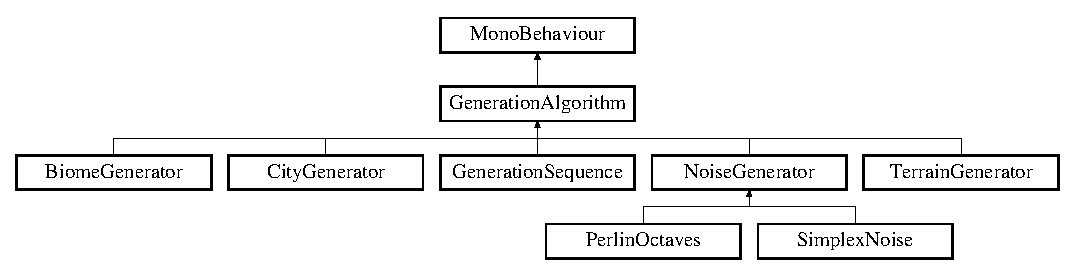
\includegraphics[height=3.246377cm]{class_generation_algorithm}
\end{center}
\end{figure}
\subsection*{Public Member Functions}
\begin{DoxyCompactItemize}
\item 
abstract bool \mbox{\hyperlink{class_generation_algorithm_af7d03e24e3b7fecfe2ae43f06915986d}{Can\+Generate}} ()
\begin{DoxyCompactList}\small\item\em Checks to see if generation prerequisites are met. \end{DoxyCompactList}\item 
abstract void \mbox{\hyperlink{class_generation_algorithm_a5e891b08f0c1d8f4ccc9ad06667691ec}{Setup}} ()
\begin{DoxyCompactList}\small\item\em Collects any prerequisites for generation. \end{DoxyCompactList}\item 
virtual void \mbox{\hyperlink{class_generation_algorithm_a9c0cc2cf748d7320651aa8d48d81c407}{Generate}} (bool Should\+Invoke\+On\+Complete)
\begin{DoxyCompactList}\small\item\em Invokes On\+Generation\+Complete when finished. \end{DoxyCompactList}\item 
abstract void \mbox{\hyperlink{class_generation_algorithm_ac2df20f7751c1b480ab958791d5c7d41}{Generate}} ()
\end{DoxyCompactItemize}
\subsection*{Public Attributes}
\begin{DoxyCompactItemize}
\item 
Unity\+Event \mbox{\hyperlink{class_generation_algorithm_a2f1af71393895b242a38b22e9e69b295}{On\+Generation\+Complete}}
\end{DoxyCompactItemize}


\subsection{Detailed Description}
Wrapper for various generation algorithms that adds events. 

\subsection{Member Function Documentation}
\mbox{\Hypertarget{class_generation_algorithm_af7d03e24e3b7fecfe2ae43f06915986d}\label{class_generation_algorithm_af7d03e24e3b7fecfe2ae43f06915986d}} 
\index{Generation\+Algorithm@{Generation\+Algorithm}!Can\+Generate@{Can\+Generate}}
\index{Can\+Generate@{Can\+Generate}!Generation\+Algorithm@{Generation\+Algorithm}}
\subsubsection{\texorpdfstring{Can\+Generate()}{CanGenerate()}}
{\footnotesize\ttfamily abstract bool Generation\+Algorithm.\+Can\+Generate (\begin{DoxyParamCaption}{ }\end{DoxyParamCaption})\hspace{0.3cm}{\ttfamily [pure virtual]}}



Checks to see if generation prerequisites are met. 

\begin{DoxyReturn}{Returns}
true if ready for generation.
\end{DoxyReturn}


Implemented in \mbox{\hyperlink{class_noise_generator_a9f6eefc7403c8d228dc1752086e8c745}{Noise\+Generator}}, \mbox{\hyperlink{class_generation_sequence_a33000b1383e18a453a592ed05a9e5e56}{Generation\+Sequence}}, \mbox{\hyperlink{class_terrain_generator_aecef659ebcfc0b012f4f8eb42e11f337}{Terrain\+Generator}}, \mbox{\hyperlink{class_city_generator_abae83261cf4eea2ed07339b644ed13af}{City\+Generator}}, and \mbox{\hyperlink{class_biome_generator_abe3d21283eef52d4c3ae631178ab69fc}{Biome\+Generator}}.

\mbox{\Hypertarget{class_generation_algorithm_a9c0cc2cf748d7320651aa8d48d81c407}\label{class_generation_algorithm_a9c0cc2cf748d7320651aa8d48d81c407}} 
\index{Generation\+Algorithm@{Generation\+Algorithm}!Generate@{Generate}}
\index{Generate@{Generate}!Generation\+Algorithm@{Generation\+Algorithm}}
\subsubsection{\texorpdfstring{Generate()}{Generate()}\hspace{0.1cm}{\footnotesize\ttfamily [1/2]}}
{\footnotesize\ttfamily virtual void Generation\+Algorithm.\+Generate (\begin{DoxyParamCaption}\item[{bool}]{Should\+Invoke\+On\+Complete }\end{DoxyParamCaption})\hspace{0.3cm}{\ttfamily [virtual]}}



Invokes On\+Generation\+Complete when finished. 

\mbox{\Hypertarget{class_generation_algorithm_ac2df20f7751c1b480ab958791d5c7d41}\label{class_generation_algorithm_ac2df20f7751c1b480ab958791d5c7d41}} 
\index{Generation\+Algorithm@{Generation\+Algorithm}!Generate@{Generate}}
\index{Generate@{Generate}!Generation\+Algorithm@{Generation\+Algorithm}}
\subsubsection{\texorpdfstring{Generate()}{Generate()}\hspace{0.1cm}{\footnotesize\ttfamily [2/2]}}
{\footnotesize\ttfamily abstract void Generation\+Algorithm.\+Generate (\begin{DoxyParamCaption}{ }\end{DoxyParamCaption})\hspace{0.3cm}{\ttfamily [pure virtual]}}



Implemented in \mbox{\hyperlink{class_terrain_generator_ace92d2a3406204b124c51e91f68a0aec}{Terrain\+Generator}}, \mbox{\hyperlink{class_noise_generator_af97b78b12d39a0ae2d05e1d28c970005}{Noise\+Generator}}, \mbox{\hyperlink{class_generation_sequence_ac594b809365f2af5e423bfd5830b796a}{Generation\+Sequence}}, \mbox{\hyperlink{class_city_generator_aa80ad8d8d723fd17f6bf9a4fe89dec4f}{City\+Generator}}, and \mbox{\hyperlink{class_biome_generator_ac8ac31b6e0276662994f0cd143457fdb}{Biome\+Generator}}.

\mbox{\Hypertarget{class_generation_algorithm_a5e891b08f0c1d8f4ccc9ad06667691ec}\label{class_generation_algorithm_a5e891b08f0c1d8f4ccc9ad06667691ec}} 
\index{Generation\+Algorithm@{Generation\+Algorithm}!Setup@{Setup}}
\index{Setup@{Setup}!Generation\+Algorithm@{Generation\+Algorithm}}
\subsubsection{\texorpdfstring{Setup()}{Setup()}}
{\footnotesize\ttfamily abstract void Generation\+Algorithm.\+Setup (\begin{DoxyParamCaption}{ }\end{DoxyParamCaption})\hspace{0.3cm}{\ttfamily [pure virtual]}}



Collects any prerequisites for generation. 



Implemented in \mbox{\hyperlink{class_simplex_noise_a43164ec5960921789ce75e83651717cf}{Simplex\+Noise}}, \mbox{\hyperlink{class_noise_generator_ad87355d424b537a1a4065d525ec18400}{Noise\+Generator}}, \mbox{\hyperlink{class_terrain_generator_ada250260b370382c1ba5cad243a67f10}{Terrain\+Generator}}, \mbox{\hyperlink{class_generation_sequence_ad433bd211eb9ed7e39d6e354c40289ff}{Generation\+Sequence}}, \mbox{\hyperlink{class_biome_generator_aa1df38909c58ff7112ebfd285e65f6c0}{Biome\+Generator}}, and \mbox{\hyperlink{class_city_generator_a1b17b4a2ea1d8a4cc1b320829da286ae}{City\+Generator}}.



\subsection{Member Data Documentation}
\mbox{\Hypertarget{class_generation_algorithm_a2f1af71393895b242a38b22e9e69b295}\label{class_generation_algorithm_a2f1af71393895b242a38b22e9e69b295}} 
\index{Generation\+Algorithm@{Generation\+Algorithm}!On\+Generation\+Complete@{On\+Generation\+Complete}}
\index{On\+Generation\+Complete@{On\+Generation\+Complete}!Generation\+Algorithm@{Generation\+Algorithm}}
\subsubsection{\texorpdfstring{On\+Generation\+Complete}{OnGenerationComplete}}
{\footnotesize\ttfamily Unity\+Event Generation\+Algorithm.\+On\+Generation\+Complete}



The documentation for this class was generated from the following file\+:\begin{DoxyCompactItemize}
\item 
/\+Users/sabienambrose/\+Documents/\+Coding/\+Unity\+Mechanical\+Turk/\+Mechanical\+Turk/\+Assets/\+Scripts/\+Framework/\+Generation/\mbox{\hyperlink{_generation_algorithm_8cs}{Generation\+Algorithm.\+cs}}\end{DoxyCompactItemize}

\hypertarget{class_generation_controller}{}\section{Generation\+Controller Class Reference}
\label{class_generation_controller}\index{Generation\+Controller@{Generation\+Controller}}


Manages Random Seed, Generation Sequences.  


Inheritance diagram for Generation\+Controller\+:\begin{figure}[H]
\begin{center}
\leavevmode
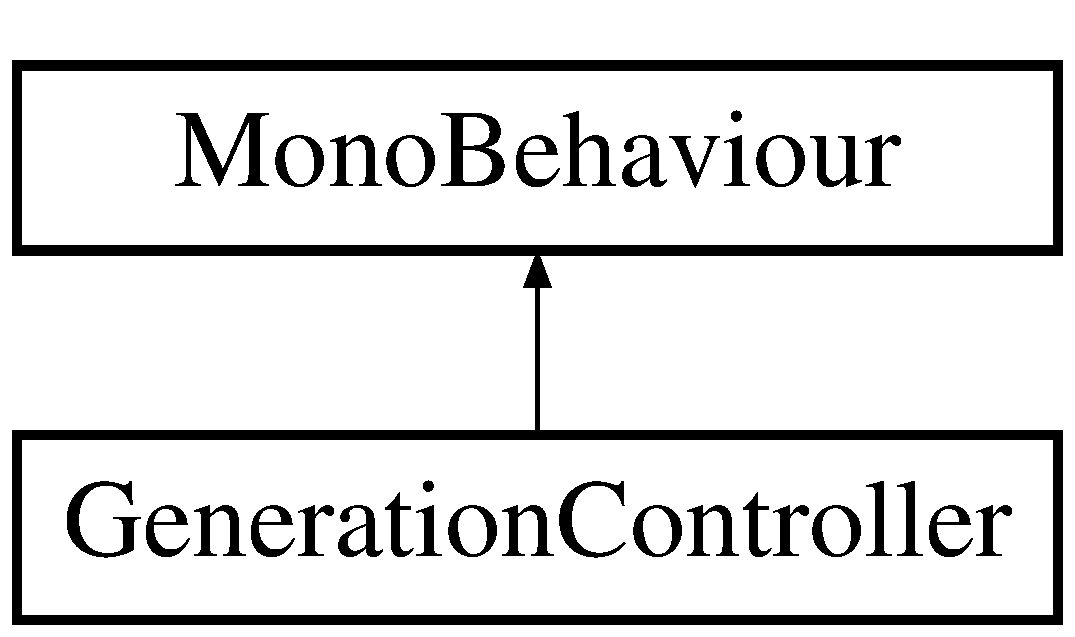
\includegraphics[height=2.000000cm]{class_generation_controller}
\end{center}
\end{figure}
\subsection*{Public Member Functions}
\begin{DoxyCompactItemize}
\item 
virtual void \mbox{\hyperlink{class_generation_controller_acd448bb5172dac81bd23d5adf5bf10b4}{Start\+Generation\+Sequence}} ()
\item 
void \mbox{\hyperlink{class_generation_controller_ab27f15ea71ed914f3ab494a7d99bb14f}{Generate\+Heightmap}} ()
\item 
void \mbox{\hyperlink{class_generation_controller_a45c2cd12e416dd1445b5182a6a2a7693}{Generate\+City}} ()
\item 
void \mbox{\hyperlink{class_generation_controller_a3588a2d352dbd2edfef4f9380207cf6c}{Setup\+And\+Generate}} ()
\end{DoxyCompactItemize}
\subsection*{Public Attributes}
\begin{DoxyCompactItemize}
\item 
int \mbox{\hyperlink{class_generation_controller_a8fc1d7ff7316969411545d4b4a7a547a}{Seed}}
\item 
\mbox{\hyperlink{class_terrain_generator}{Terrain\+Generator}} \mbox{\hyperlink{class_generation_controller_aca0b988596dc14d92fdbd9fb5037c2cd}{terrain\+Generator}}
\item 
\mbox{\hyperlink{class_city_generator}{City\+Generator}} \mbox{\hyperlink{class_generation_controller_a215ad934a6c4951844954b6b61b0187d}{city\+Generator}}
\end{DoxyCompactItemize}
\subsection*{Protected Member Functions}
\begin{DoxyCompactItemize}
\item 
virtual void \mbox{\hyperlink{class_generation_controller_a178f4eb6bcb5cbe94a7d67cb8685857f}{Look\+For\+Components}} ()
\item 
virtual void \mbox{\hyperlink{class_generation_controller_acc6ec4bf38f4982c3d727a36b6aed321}{Setup}} ()
\end{DoxyCompactItemize}
\subsection*{Properties}
\begin{DoxyCompactItemize}
\item 
\mbox{\hyperlink{class_noise_map}{Noise\+Map}} \mbox{\hyperlink{class_generation_controller_ada5207d54f73a82b066d367a65dd6035}{height\+Map}}\hspace{0.3cm}{\ttfamily  \mbox{[}get, set\mbox{]}}
\end{DoxyCompactItemize}


\subsection{Detailed Description}
Manages Random Seed, Generation Sequences. 



\subsection{Member Function Documentation}
\mbox{\Hypertarget{class_generation_controller_a45c2cd12e416dd1445b5182a6a2a7693}\label{class_generation_controller_a45c2cd12e416dd1445b5182a6a2a7693}} 
\index{Generation\+Controller@{Generation\+Controller}!Generate\+City@{Generate\+City}}
\index{Generate\+City@{Generate\+City}!Generation\+Controller@{Generation\+Controller}}
\subsubsection{\texorpdfstring{Generate\+City()}{GenerateCity()}}
{\footnotesize\ttfamily void Generation\+Controller.\+Generate\+City (\begin{DoxyParamCaption}{ }\end{DoxyParamCaption})}

\mbox{\Hypertarget{class_generation_controller_ab27f15ea71ed914f3ab494a7d99bb14f}\label{class_generation_controller_ab27f15ea71ed914f3ab494a7d99bb14f}} 
\index{Generation\+Controller@{Generation\+Controller}!Generate\+Heightmap@{Generate\+Heightmap}}
\index{Generate\+Heightmap@{Generate\+Heightmap}!Generation\+Controller@{Generation\+Controller}}
\subsubsection{\texorpdfstring{Generate\+Heightmap()}{GenerateHeightmap()}}
{\footnotesize\ttfamily void Generation\+Controller.\+Generate\+Heightmap (\begin{DoxyParamCaption}{ }\end{DoxyParamCaption})}

\mbox{\Hypertarget{class_generation_controller_a178f4eb6bcb5cbe94a7d67cb8685857f}\label{class_generation_controller_a178f4eb6bcb5cbe94a7d67cb8685857f}} 
\index{Generation\+Controller@{Generation\+Controller}!Look\+For\+Components@{Look\+For\+Components}}
\index{Look\+For\+Components@{Look\+For\+Components}!Generation\+Controller@{Generation\+Controller}}
\subsubsection{\texorpdfstring{Look\+For\+Components()}{LookForComponents()}}
{\footnotesize\ttfamily virtual void Generation\+Controller.\+Look\+For\+Components (\begin{DoxyParamCaption}{ }\end{DoxyParamCaption})\hspace{0.3cm}{\ttfamily [protected]}, {\ttfamily [virtual]}}

\mbox{\Hypertarget{class_generation_controller_acc6ec4bf38f4982c3d727a36b6aed321}\label{class_generation_controller_acc6ec4bf38f4982c3d727a36b6aed321}} 
\index{Generation\+Controller@{Generation\+Controller}!Setup@{Setup}}
\index{Setup@{Setup}!Generation\+Controller@{Generation\+Controller}}
\subsubsection{\texorpdfstring{Setup()}{Setup()}}
{\footnotesize\ttfamily virtual void Generation\+Controller.\+Setup (\begin{DoxyParamCaption}{ }\end{DoxyParamCaption})\hspace{0.3cm}{\ttfamily [protected]}, {\ttfamily [virtual]}}

\mbox{\Hypertarget{class_generation_controller_a3588a2d352dbd2edfef4f9380207cf6c}\label{class_generation_controller_a3588a2d352dbd2edfef4f9380207cf6c}} 
\index{Generation\+Controller@{Generation\+Controller}!Setup\+And\+Generate@{Setup\+And\+Generate}}
\index{Setup\+And\+Generate@{Setup\+And\+Generate}!Generation\+Controller@{Generation\+Controller}}
\subsubsection{\texorpdfstring{Setup\+And\+Generate()}{SetupAndGenerate()}}
{\footnotesize\ttfamily void Generation\+Controller.\+Setup\+And\+Generate (\begin{DoxyParamCaption}{ }\end{DoxyParamCaption})}

\mbox{\Hypertarget{class_generation_controller_acd448bb5172dac81bd23d5adf5bf10b4}\label{class_generation_controller_acd448bb5172dac81bd23d5adf5bf10b4}} 
\index{Generation\+Controller@{Generation\+Controller}!Start\+Generation\+Sequence@{Start\+Generation\+Sequence}}
\index{Start\+Generation\+Sequence@{Start\+Generation\+Sequence}!Generation\+Controller@{Generation\+Controller}}
\subsubsection{\texorpdfstring{Start\+Generation\+Sequence()}{StartGenerationSequence()}}
{\footnotesize\ttfamily virtual void Generation\+Controller.\+Start\+Generation\+Sequence (\begin{DoxyParamCaption}{ }\end{DoxyParamCaption})\hspace{0.3cm}{\ttfamily [virtual]}}



\subsection{Member Data Documentation}
\mbox{\Hypertarget{class_generation_controller_a215ad934a6c4951844954b6b61b0187d}\label{class_generation_controller_a215ad934a6c4951844954b6b61b0187d}} 
\index{Generation\+Controller@{Generation\+Controller}!city\+Generator@{city\+Generator}}
\index{city\+Generator@{city\+Generator}!Generation\+Controller@{Generation\+Controller}}
\subsubsection{\texorpdfstring{city\+Generator}{cityGenerator}}
{\footnotesize\ttfamily \mbox{\hyperlink{class_city_generator}{City\+Generator}} Generation\+Controller.\+city\+Generator}

\mbox{\Hypertarget{class_generation_controller_a8fc1d7ff7316969411545d4b4a7a547a}\label{class_generation_controller_a8fc1d7ff7316969411545d4b4a7a547a}} 
\index{Generation\+Controller@{Generation\+Controller}!Seed@{Seed}}
\index{Seed@{Seed}!Generation\+Controller@{Generation\+Controller}}
\subsubsection{\texorpdfstring{Seed}{Seed}}
{\footnotesize\ttfamily int Generation\+Controller.\+Seed}

\mbox{\Hypertarget{class_generation_controller_aca0b988596dc14d92fdbd9fb5037c2cd}\label{class_generation_controller_aca0b988596dc14d92fdbd9fb5037c2cd}} 
\index{Generation\+Controller@{Generation\+Controller}!terrain\+Generator@{terrain\+Generator}}
\index{terrain\+Generator@{terrain\+Generator}!Generation\+Controller@{Generation\+Controller}}
\subsubsection{\texorpdfstring{terrain\+Generator}{terrainGenerator}}
{\footnotesize\ttfamily \mbox{\hyperlink{class_terrain_generator}{Terrain\+Generator}} Generation\+Controller.\+terrain\+Generator}



\subsection{Property Documentation}
\mbox{\Hypertarget{class_generation_controller_ada5207d54f73a82b066d367a65dd6035}\label{class_generation_controller_ada5207d54f73a82b066d367a65dd6035}} 
\index{Generation\+Controller@{Generation\+Controller}!height\+Map@{height\+Map}}
\index{height\+Map@{height\+Map}!Generation\+Controller@{Generation\+Controller}}
\subsubsection{\texorpdfstring{height\+Map}{heightMap}}
{\footnotesize\ttfamily \mbox{\hyperlink{class_noise_map}{Noise\+Map}} Generation\+Controller.\+height\+Map\hspace{0.3cm}{\ttfamily [get]}, {\ttfamily [set]}}



The documentation for this class was generated from the following file\+:\begin{DoxyCompactItemize}
\item 
/\+Users/sabienambrose/\+Documents/\+Coding/\+Unity\+Mechanical\+Turk/\+Mechanical\+Turk/\+Assets/\+Scripts/\+Framework/\+Generation/\mbox{\hyperlink{_generation_controller_8cs}{Generation\+Controller.\+cs}}\end{DoxyCompactItemize}

\hypertarget{class_generation_sequence}{}\section{Generation\+Sequence Class Reference}
\label{class_generation_sequence}\index{Generation\+Sequence@{Generation\+Sequence}}
Inheritance diagram for Generation\+Sequence\+:\begin{figure}[H]
\begin{center}
\leavevmode
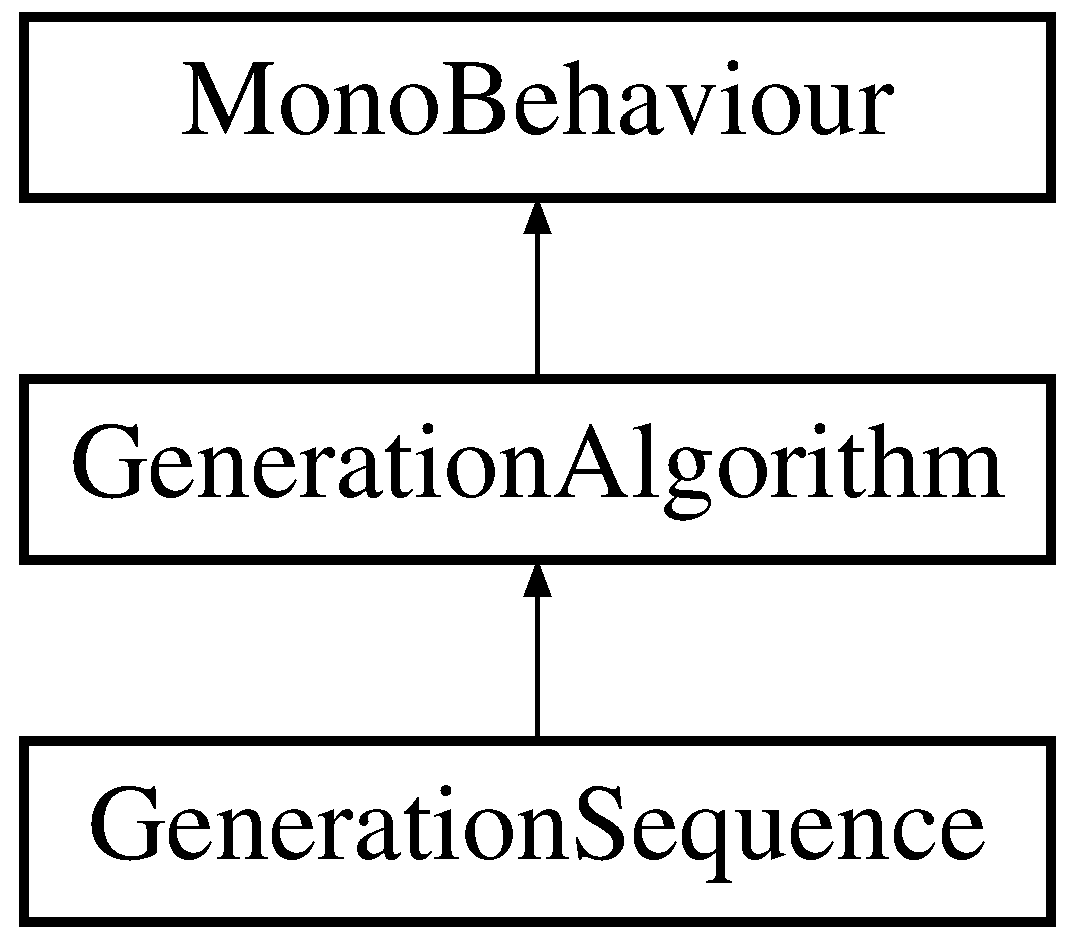
\includegraphics[height=3.000000cm]{class_generation_sequence}
\end{center}
\end{figure}
\subsection*{Public Member Functions}
\begin{DoxyCompactItemize}
\item 
\mbox{\hyperlink{class_generation_algorithm}{Generation\+Algorithm}} \mbox{\hyperlink{class_generation_sequence_a09f98429afb3efcaa424397d45847132}{Get\+Current\+Algorithm}} ()
\item 
override bool \mbox{\hyperlink{class_generation_sequence_a33000b1383e18a453a592ed05a9e5e56}{Can\+Generate}} ()
\begin{DoxyCompactList}\small\item\em Checks to see if generation prerequisites are met. \end{DoxyCompactList}\item 
override void \mbox{\hyperlink{class_generation_sequence_ad433bd211eb9ed7e39d6e354c40289ff}{Setup}} ()
\begin{DoxyCompactList}\small\item\em Collects any prerequisites for generation. \end{DoxyCompactList}\item 
virtual void \mbox{\hyperlink{class_generation_sequence_afdce2edf1188afcaf018d67010c127c4}{Start\+Next\+Algorithm}} ()
\begin{DoxyCompactList}\small\item\em Increments  and calls Start\+Current\+Algorithm \end{DoxyCompactList}\item 
override void \mbox{\hyperlink{class_generation_sequence_ac594b809365f2af5e423bfd5830b796a}{Generate}} ()
\end{DoxyCompactItemize}
\subsection*{Public Attributes}
\begin{DoxyCompactItemize}
\item 
List$<$ \mbox{\hyperlink{class_generation_algorithm}{Generation\+Algorithm}} $>$ \mbox{\hyperlink{class_generation_sequence_a4e4b450952479c6d089c47ad514f15ae}{generation\+Sequence}} = new List$<$\mbox{\hyperlink{class_generation_algorithm}{Generation\+Algorithm}}$>$()
\item 
int \mbox{\hyperlink{class_generation_sequence_ad8f5b50dde07c78b79462dcd23b7cfde}{seq\+Index}}
\end{DoxyCompactItemize}


\subsection{Member Function Documentation}
\mbox{\Hypertarget{class_generation_sequence_a33000b1383e18a453a592ed05a9e5e56}\label{class_generation_sequence_a33000b1383e18a453a592ed05a9e5e56}} 
\index{Generation\+Sequence@{Generation\+Sequence}!Can\+Generate@{Can\+Generate}}
\index{Can\+Generate@{Can\+Generate}!Generation\+Sequence@{Generation\+Sequence}}
\subsubsection{\texorpdfstring{Can\+Generate()}{CanGenerate()}}
{\footnotesize\ttfamily override bool Generation\+Sequence.\+Can\+Generate (\begin{DoxyParamCaption}{ }\end{DoxyParamCaption})\hspace{0.3cm}{\ttfamily [virtual]}}



Checks to see if generation prerequisites are met. 

\begin{DoxyReturn}{Returns}
true if ready for generation.
\end{DoxyReturn}


Implements \mbox{\hyperlink{class_generation_algorithm_af7d03e24e3b7fecfe2ae43f06915986d}{Generation\+Algorithm}}.

\mbox{\Hypertarget{class_generation_sequence_ac594b809365f2af5e423bfd5830b796a}\label{class_generation_sequence_ac594b809365f2af5e423bfd5830b796a}} 
\index{Generation\+Sequence@{Generation\+Sequence}!Generate@{Generate}}
\index{Generate@{Generate}!Generation\+Sequence@{Generation\+Sequence}}
\subsubsection{\texorpdfstring{Generate()}{Generate()}}
{\footnotesize\ttfamily override void Generation\+Sequence.\+Generate (\begin{DoxyParamCaption}{ }\end{DoxyParamCaption})\hspace{0.3cm}{\ttfamily [virtual]}}



Implements \mbox{\hyperlink{class_generation_algorithm_ac2df20f7751c1b480ab958791d5c7d41}{Generation\+Algorithm}}.

\mbox{\Hypertarget{class_generation_sequence_a09f98429afb3efcaa424397d45847132}\label{class_generation_sequence_a09f98429afb3efcaa424397d45847132}} 
\index{Generation\+Sequence@{Generation\+Sequence}!Get\+Current\+Algorithm@{Get\+Current\+Algorithm}}
\index{Get\+Current\+Algorithm@{Get\+Current\+Algorithm}!Generation\+Sequence@{Generation\+Sequence}}
\subsubsection{\texorpdfstring{Get\+Current\+Algorithm()}{GetCurrentAlgorithm()}}
{\footnotesize\ttfamily \mbox{\hyperlink{class_generation_algorithm}{Generation\+Algorithm}} Generation\+Sequence.\+Get\+Current\+Algorithm (\begin{DoxyParamCaption}{ }\end{DoxyParamCaption})}

\mbox{\Hypertarget{class_generation_sequence_ad433bd211eb9ed7e39d6e354c40289ff}\label{class_generation_sequence_ad433bd211eb9ed7e39d6e354c40289ff}} 
\index{Generation\+Sequence@{Generation\+Sequence}!Setup@{Setup}}
\index{Setup@{Setup}!Generation\+Sequence@{Generation\+Sequence}}
\subsubsection{\texorpdfstring{Setup()}{Setup()}}
{\footnotesize\ttfamily override void Generation\+Sequence.\+Setup (\begin{DoxyParamCaption}{ }\end{DoxyParamCaption})\hspace{0.3cm}{\ttfamily [virtual]}}



Collects any prerequisites for generation. 



Implements \mbox{\hyperlink{class_generation_algorithm_a5e891b08f0c1d8f4ccc9ad06667691ec}{Generation\+Algorithm}}.

\mbox{\Hypertarget{class_generation_sequence_afdce2edf1188afcaf018d67010c127c4}\label{class_generation_sequence_afdce2edf1188afcaf018d67010c127c4}} 
\index{Generation\+Sequence@{Generation\+Sequence}!Start\+Next\+Algorithm@{Start\+Next\+Algorithm}}
\index{Start\+Next\+Algorithm@{Start\+Next\+Algorithm}!Generation\+Sequence@{Generation\+Sequence}}
\subsubsection{\texorpdfstring{Start\+Next\+Algorithm()}{StartNextAlgorithm()}}
{\footnotesize\ttfamily virtual void Generation\+Sequence.\+Start\+Next\+Algorithm (\begin{DoxyParamCaption}{ }\end{DoxyParamCaption})\hspace{0.3cm}{\ttfamily [virtual]}}



Increments  and calls Start\+Current\+Algorithm 



\subsection{Member Data Documentation}
\mbox{\Hypertarget{class_generation_sequence_a4e4b450952479c6d089c47ad514f15ae}\label{class_generation_sequence_a4e4b450952479c6d089c47ad514f15ae}} 
\index{Generation\+Sequence@{Generation\+Sequence}!generation\+Sequence@{generation\+Sequence}}
\index{generation\+Sequence@{generation\+Sequence}!Generation\+Sequence@{Generation\+Sequence}}
\subsubsection{\texorpdfstring{generation\+Sequence}{generationSequence}}
{\footnotesize\ttfamily List$<$\mbox{\hyperlink{class_generation_algorithm}{Generation\+Algorithm}}$>$ Generation\+Sequence.\+generation\+Sequence = new List$<$\mbox{\hyperlink{class_generation_algorithm}{Generation\+Algorithm}}$>$()}

\mbox{\Hypertarget{class_generation_sequence_ad8f5b50dde07c78b79462dcd23b7cfde}\label{class_generation_sequence_ad8f5b50dde07c78b79462dcd23b7cfde}} 
\index{Generation\+Sequence@{Generation\+Sequence}!seq\+Index@{seq\+Index}}
\index{seq\+Index@{seq\+Index}!Generation\+Sequence@{Generation\+Sequence}}
\subsubsection{\texorpdfstring{seq\+Index}{seqIndex}}
{\footnotesize\ttfamily int Generation\+Sequence.\+seq\+Index}



The documentation for this class was generated from the following file\+:\begin{DoxyCompactItemize}
\item 
/\+Users/sabienambrose/\+Documents/\+Coding/\+Unity\+Mechanical\+Turk/\+Mechanical\+Turk/\+Assets/\+Scripts/\+Framework/\+Generation/\mbox{\hyperlink{_generation_sequence_8cs}{Generation\+Sequence.\+cs}}\end{DoxyCompactItemize}

\hypertarget{class_simplex_noise_1_1_grad}{}\section{Simplex\+Noise.\+Grad Class Reference}
\label{class_simplex_noise_1_1_grad}\index{Simplex\+Noise.\+Grad@{Simplex\+Noise.\+Grad}}
\subsection*{Public Member Functions}
\begin{DoxyCompactItemize}
\item 
\mbox{\hyperlink{class_simplex_noise_1_1_grad_a079ab55e913e9e7a152bddede45dfa55}{Grad}} (float \mbox{\hyperlink{class_simplex_noise_1_1_grad_a623740b94dbbf25b8fd4df3a14ed6cc5}{x}}, float y)
\end{DoxyCompactItemize}
\subsection*{Public Attributes}
\begin{DoxyCompactItemize}
\item 
float \mbox{\hyperlink{class_simplex_noise_1_1_grad_a623740b94dbbf25b8fd4df3a14ed6cc5}{x}}
\end{DoxyCompactItemize}


\subsection{Constructor \& Destructor Documentation}
\mbox{\Hypertarget{class_simplex_noise_1_1_grad_a079ab55e913e9e7a152bddede45dfa55}\label{class_simplex_noise_1_1_grad_a079ab55e913e9e7a152bddede45dfa55}} 
\index{Simplex\+Noise\+::\+Grad@{Simplex\+Noise\+::\+Grad}!Grad@{Grad}}
\index{Grad@{Grad}!Simplex\+Noise\+::\+Grad@{Simplex\+Noise\+::\+Grad}}
\subsubsection{\texorpdfstring{Grad()}{Grad()}}
{\footnotesize\ttfamily Simplex\+Noise.\+Grad.\+Grad (\begin{DoxyParamCaption}\item[{float}]{x,  }\item[{float}]{y }\end{DoxyParamCaption})}



\subsection{Member Data Documentation}
\mbox{\Hypertarget{class_simplex_noise_1_1_grad_a623740b94dbbf25b8fd4df3a14ed6cc5}\label{class_simplex_noise_1_1_grad_a623740b94dbbf25b8fd4df3a14ed6cc5}} 
\index{Simplex\+Noise\+::\+Grad@{Simplex\+Noise\+::\+Grad}!x@{x}}
\index{x@{x}!Simplex\+Noise\+::\+Grad@{Simplex\+Noise\+::\+Grad}}
\subsubsection{\texorpdfstring{x}{x}}
{\footnotesize\ttfamily float Simplex\+Noise.\+Grad.\+x}



The documentation for this class was generated from the following file\+:\begin{DoxyCompactItemize}
\item 
/\+Users/sabienambrose/\+Documents/\+Coding/\+Unity\+Mechanical\+Turk/\+Mechanical\+Turk/\+Assets/\+Scripts/\+Generation/\+Noise/\mbox{\hyperlink{_simplex_noise_8cs}{Simplex\+Noise.\+cs}}\end{DoxyCompactItemize}

\hypertarget{class_graph_builder}{}\section{Graph\+Builder Class Reference}
\label{class_graph_builder}\index{Graph\+Builder@{Graph\+Builder}}
Inheritance diagram for Graph\+Builder\+:\begin{figure}[H]
\begin{center}
\leavevmode
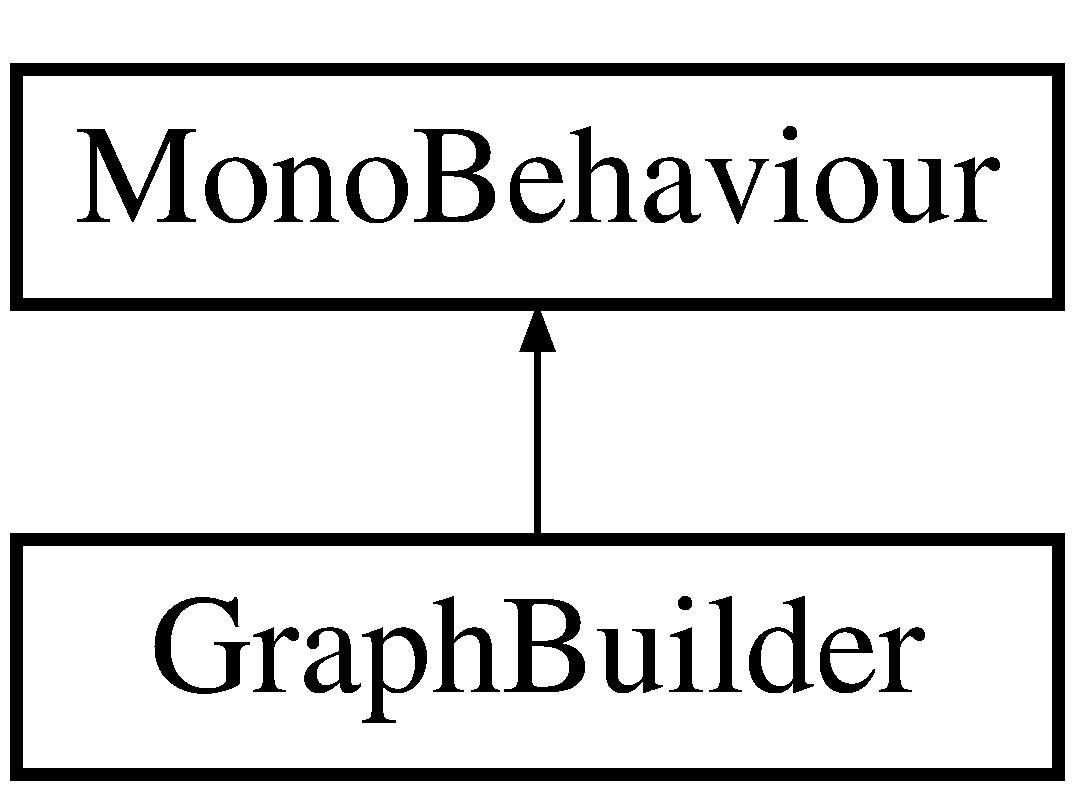
\includegraphics[height=2.000000cm]{class_graph_builder}
\end{center}
\end{figure}
\subsection*{Public Member Functions}
\begin{DoxyCompactItemize}
\item 
void \mbox{\hyperlink{class_graph_builder_a8297aa8425e28706cebf248501a7ddd9}{Start}} ()
\item 
void \mbox{\hyperlink{class_graph_builder_aa6d73ad673971862998c257818424b15}{Init}} ()
\item 
void \mbox{\hyperlink{class_graph_builder_ae9977fd7ab38bdc105ffef8898e1aa99}{Initialize\+Graph}} ()
\item 
void \mbox{\hyperlink{class_graph_builder_a45ab6fb54d2778b4c9b3c02f5b8aaa92}{Next\+Point}} ()
\item 
void \mbox{\hyperlink{class_graph_builder_aa6347d6e481e9bc58f3378edd8f00cfa}{Fill\+Points}} ()
\item 
void \mbox{\hyperlink{class_graph_builder_af5ad417df74a878c05b2b3f0350603af}{Update\+Mesh\+Data}} ()
\item 
void \mbox{\hyperlink{class_graph_builder_a5f073a99b5be732e8ea1ac4f40858d41}{Create\+Meshes\+From\+Faces}} (Mesh mesh)
\end{DoxyCompactItemize}
\subsection*{Public Attributes}
\begin{DoxyCompactItemize}
\item 
\mbox{\hyperlink{class_delaunay_triangulation}{Delaunay\+Triangulation}} \mbox{\hyperlink{class_graph_builder_a4fbe227325c986a86af9d4b813036dcc}{del\+Tri}}
\item 
bool \mbox{\hyperlink{class_graph_builder_aacf2833ccc9ae6f68197e594ed8b3183}{draw\+Triangles}} = false
\item 
\mbox{\hyperlink{class_point_generator}{Point\+Generator}} \mbox{\hyperlink{class_graph_builder_a621748ddd5e210bde566ddf1bffa1bbe}{point\+Generator}}
\item 
bool \mbox{\hyperlink{class_graph_builder_a0acb80a89e2f7cfdaad969d6a858c832}{draw\+Points}} = true
\item 
\mbox{\hyperlink{class_poly_grid}{Poly\+Grid}} \mbox{\hyperlink{class_graph_builder_afc729c2338a301483a3f96e6106799bb}{poly\+Grid}}
\item 
Game\+Object \mbox{[}$\,$\mbox{]} \mbox{\hyperlink{class_graph_builder_a0b87acbb20c7641e19a499818a100e8a}{L\+O\+D\+\_\+0\+\_\+\+Prefabs}} = new Game\+Object\mbox{[}3\mbox{]}
\end{DoxyCompactItemize}


\subsection{Member Function Documentation}
\mbox{\Hypertarget{class_graph_builder_a5f073a99b5be732e8ea1ac4f40858d41}\label{class_graph_builder_a5f073a99b5be732e8ea1ac4f40858d41}} 
\index{Graph\+Builder@{Graph\+Builder}!Create\+Meshes\+From\+Faces@{Create\+Meshes\+From\+Faces}}
\index{Create\+Meshes\+From\+Faces@{Create\+Meshes\+From\+Faces}!Graph\+Builder@{Graph\+Builder}}
\subsubsection{\texorpdfstring{Create\+Meshes\+From\+Faces()}{CreateMeshesFromFaces()}}
{\footnotesize\ttfamily void Graph\+Builder.\+Create\+Meshes\+From\+Faces (\begin{DoxyParamCaption}\item[{Mesh}]{mesh }\end{DoxyParamCaption})}

\mbox{\Hypertarget{class_graph_builder_aa6347d6e481e9bc58f3378edd8f00cfa}\label{class_graph_builder_aa6347d6e481e9bc58f3378edd8f00cfa}} 
\index{Graph\+Builder@{Graph\+Builder}!Fill\+Points@{Fill\+Points}}
\index{Fill\+Points@{Fill\+Points}!Graph\+Builder@{Graph\+Builder}}
\subsubsection{\texorpdfstring{Fill\+Points()}{FillPoints()}}
{\footnotesize\ttfamily void Graph\+Builder.\+Fill\+Points (\begin{DoxyParamCaption}{ }\end{DoxyParamCaption})}

\mbox{\Hypertarget{class_graph_builder_aa6d73ad673971862998c257818424b15}\label{class_graph_builder_aa6d73ad673971862998c257818424b15}} 
\index{Graph\+Builder@{Graph\+Builder}!Init@{Init}}
\index{Init@{Init}!Graph\+Builder@{Graph\+Builder}}
\subsubsection{\texorpdfstring{Init()}{Init()}}
{\footnotesize\ttfamily void Graph\+Builder.\+Init (\begin{DoxyParamCaption}{ }\end{DoxyParamCaption})}

\mbox{\Hypertarget{class_graph_builder_ae9977fd7ab38bdc105ffef8898e1aa99}\label{class_graph_builder_ae9977fd7ab38bdc105ffef8898e1aa99}} 
\index{Graph\+Builder@{Graph\+Builder}!Initialize\+Graph@{Initialize\+Graph}}
\index{Initialize\+Graph@{Initialize\+Graph}!Graph\+Builder@{Graph\+Builder}}
\subsubsection{\texorpdfstring{Initialize\+Graph()}{InitializeGraph()}}
{\footnotesize\ttfamily void Graph\+Builder.\+Initialize\+Graph (\begin{DoxyParamCaption}{ }\end{DoxyParamCaption})}

\mbox{\Hypertarget{class_graph_builder_a45ab6fb54d2778b4c9b3c02f5b8aaa92}\label{class_graph_builder_a45ab6fb54d2778b4c9b3c02f5b8aaa92}} 
\index{Graph\+Builder@{Graph\+Builder}!Next\+Point@{Next\+Point}}
\index{Next\+Point@{Next\+Point}!Graph\+Builder@{Graph\+Builder}}
\subsubsection{\texorpdfstring{Next\+Point()}{NextPoint()}}
{\footnotesize\ttfamily void Graph\+Builder.\+Next\+Point (\begin{DoxyParamCaption}{ }\end{DoxyParamCaption})}

\mbox{\Hypertarget{class_graph_builder_a8297aa8425e28706cebf248501a7ddd9}\label{class_graph_builder_a8297aa8425e28706cebf248501a7ddd9}} 
\index{Graph\+Builder@{Graph\+Builder}!Start@{Start}}
\index{Start@{Start}!Graph\+Builder@{Graph\+Builder}}
\subsubsection{\texorpdfstring{Start()}{Start()}}
{\footnotesize\ttfamily void Graph\+Builder.\+Start (\begin{DoxyParamCaption}{ }\end{DoxyParamCaption})}

\mbox{\Hypertarget{class_graph_builder_af5ad417df74a878c05b2b3f0350603af}\label{class_graph_builder_af5ad417df74a878c05b2b3f0350603af}} 
\index{Graph\+Builder@{Graph\+Builder}!Update\+Mesh\+Data@{Update\+Mesh\+Data}}
\index{Update\+Mesh\+Data@{Update\+Mesh\+Data}!Graph\+Builder@{Graph\+Builder}}
\subsubsection{\texorpdfstring{Update\+Mesh\+Data()}{UpdateMeshData()}}
{\footnotesize\ttfamily void Graph\+Builder.\+Update\+Mesh\+Data (\begin{DoxyParamCaption}{ }\end{DoxyParamCaption})}



\subsection{Member Data Documentation}
\mbox{\Hypertarget{class_graph_builder_a4fbe227325c986a86af9d4b813036dcc}\label{class_graph_builder_a4fbe227325c986a86af9d4b813036dcc}} 
\index{Graph\+Builder@{Graph\+Builder}!del\+Tri@{del\+Tri}}
\index{del\+Tri@{del\+Tri}!Graph\+Builder@{Graph\+Builder}}
\subsubsection{\texorpdfstring{del\+Tri}{delTri}}
{\footnotesize\ttfamily \mbox{\hyperlink{class_delaunay_triangulation}{Delaunay\+Triangulation}} Graph\+Builder.\+del\+Tri}

\mbox{\Hypertarget{class_graph_builder_a0acb80a89e2f7cfdaad969d6a858c832}\label{class_graph_builder_a0acb80a89e2f7cfdaad969d6a858c832}} 
\index{Graph\+Builder@{Graph\+Builder}!draw\+Points@{draw\+Points}}
\index{draw\+Points@{draw\+Points}!Graph\+Builder@{Graph\+Builder}}
\subsubsection{\texorpdfstring{draw\+Points}{drawPoints}}
{\footnotesize\ttfamily bool Graph\+Builder.\+draw\+Points = true}

\mbox{\Hypertarget{class_graph_builder_aacf2833ccc9ae6f68197e594ed8b3183}\label{class_graph_builder_aacf2833ccc9ae6f68197e594ed8b3183}} 
\index{Graph\+Builder@{Graph\+Builder}!draw\+Triangles@{draw\+Triangles}}
\index{draw\+Triangles@{draw\+Triangles}!Graph\+Builder@{Graph\+Builder}}
\subsubsection{\texorpdfstring{draw\+Triangles}{drawTriangles}}
{\footnotesize\ttfamily bool Graph\+Builder.\+draw\+Triangles = false}

\mbox{\Hypertarget{class_graph_builder_a0b87acbb20c7641e19a499818a100e8a}\label{class_graph_builder_a0b87acbb20c7641e19a499818a100e8a}} 
\index{Graph\+Builder@{Graph\+Builder}!L\+O\+D\+\_\+0\+\_\+\+Prefabs@{L\+O\+D\+\_\+0\+\_\+\+Prefabs}}
\index{L\+O\+D\+\_\+0\+\_\+\+Prefabs@{L\+O\+D\+\_\+0\+\_\+\+Prefabs}!Graph\+Builder@{Graph\+Builder}}
\subsubsection{\texorpdfstring{L\+O\+D\+\_\+0\+\_\+\+Prefabs}{LOD\_0\_Prefabs}}
{\footnotesize\ttfamily Game\+Object \mbox{[}$\,$\mbox{]} Graph\+Builder.\+L\+O\+D\+\_\+0\+\_\+\+Prefabs = new Game\+Object\mbox{[}3\mbox{]}}

\mbox{\Hypertarget{class_graph_builder_a621748ddd5e210bde566ddf1bffa1bbe}\label{class_graph_builder_a621748ddd5e210bde566ddf1bffa1bbe}} 
\index{Graph\+Builder@{Graph\+Builder}!point\+Generator@{point\+Generator}}
\index{point\+Generator@{point\+Generator}!Graph\+Builder@{Graph\+Builder}}
\subsubsection{\texorpdfstring{point\+Generator}{pointGenerator}}
{\footnotesize\ttfamily \mbox{\hyperlink{class_point_generator}{Point\+Generator}} Graph\+Builder.\+point\+Generator}

\mbox{\Hypertarget{class_graph_builder_afc729c2338a301483a3f96e6106799bb}\label{class_graph_builder_afc729c2338a301483a3f96e6106799bb}} 
\index{Graph\+Builder@{Graph\+Builder}!poly\+Grid@{poly\+Grid}}
\index{poly\+Grid@{poly\+Grid}!Graph\+Builder@{Graph\+Builder}}
\subsubsection{\texorpdfstring{poly\+Grid}{polyGrid}}
{\footnotesize\ttfamily \mbox{\hyperlink{class_poly_grid}{Poly\+Grid}} Graph\+Builder.\+poly\+Grid}



The documentation for this class was generated from the following file\+:\begin{DoxyCompactItemize}
\item 
/\+Users/sabienambrose/\+Documents/\+Coding/\+Unity\+Mechanical\+Turk/\+Mechanical\+Turk/\+Assets/\+Scripts/\+Util/\+Containers/\+Graphs/\mbox{\hyperlink{_graph_builder_8cs}{Graph\+Builder.\+cs}}\end{DoxyCompactItemize}

\hypertarget{struct_grid2_d}{}\section{Grid2D Struct Reference}
\label{struct_grid2_d}\index{Grid2D@{Grid2D}}
\subsection*{Public Member Functions}
\begin{DoxyCompactItemize}
\item 
\mbox{\hyperlink{struct_grid2_d_a8ab64aa29a75f6612241c1c6ed7d8880}{Grid2D}} (int \mbox{\hyperlink{struct_grid2_d_abe3dc5ac69835aa5f571338fbb6b5d8e}{width}}, int \mbox{\hyperlink{struct_grid2_d_ae7a732a224d7276592bbca106154016d}{height}})
\item 
int \mbox{\hyperlink{struct_grid2_d_a87f97756b42b798f0fb888407a42db7c}{Get\+Width}} ()
\item 
int \mbox{\hyperlink{struct_grid2_d_a87d2a1dc516b61b520b05a07d6af5cf7}{Get\+Height}} ()
\item 
bool \mbox{\hyperlink{struct_grid2_d_a5bab1dc86bbc11873dbea422b83c01e2}{Is\+Valid\+Coord}} (\mbox{\hyperlink{struct_int_point}{Int\+Point}} grid\+Coord)
\item 
Vector2 \mbox{\hyperlink{struct_grid2_d_a080a049e035f44790cb7200518730f6c}{Get\+Point}} (int x\+Coord, int y\+Coord)
\item 
Vector2 \mbox{\hyperlink{struct_grid2_d_a5b34f0d8b83f9fa7148f42030efb7182}{Get\+Point}} (\mbox{\hyperlink{struct_int_point}{Int\+Point}} gcoord)
\item 
void \mbox{\hyperlink{struct_grid2_d_aef80a8514e645da44457a6a2e2bb4823}{Set\+Point}} (int x, int y, Vector2 point)
\item 
void \mbox{\hyperlink{struct_grid2_d_a81023ffc43b01d97edf0ced5d946763c}{Set\+Point}} (\mbox{\hyperlink{struct_int_point}{Int\+Point}} gcoord, Vector2 point)
\item 
void \mbox{\hyperlink{struct_grid2_d_a992f70ddc78c3f9f5bc025f53cfc2059}{Square\+Around\+Point}} (\mbox{\hyperlink{struct_int_point}{Int\+Point}} point, int square\+Size, out Vector2\mbox{[},\mbox{]} square)
\end{DoxyCompactItemize}
\subsection*{Public Attributes}
\begin{DoxyCompactItemize}
\item 
int \mbox{\hyperlink{struct_grid2_d_abe3dc5ac69835aa5f571338fbb6b5d8e}{width}}
\item 
int \mbox{\hyperlink{struct_grid2_d_ae7a732a224d7276592bbca106154016d}{height}}
\end{DoxyCompactItemize}


\subsection{Constructor \& Destructor Documentation}
\mbox{\Hypertarget{struct_grid2_d_a8ab64aa29a75f6612241c1c6ed7d8880}\label{struct_grid2_d_a8ab64aa29a75f6612241c1c6ed7d8880}} 
\index{Grid2D@{Grid2D}!Grid2D@{Grid2D}}
\index{Grid2D@{Grid2D}!Grid2D@{Grid2D}}
\subsubsection{\texorpdfstring{Grid2\+D()}{Grid2D()}}
{\footnotesize\ttfamily Grid2\+D.\+Grid2D (\begin{DoxyParamCaption}\item[{int}]{width,  }\item[{int}]{height }\end{DoxyParamCaption})}



\subsection{Member Function Documentation}
\mbox{\Hypertarget{struct_grid2_d_a87d2a1dc516b61b520b05a07d6af5cf7}\label{struct_grid2_d_a87d2a1dc516b61b520b05a07d6af5cf7}} 
\index{Grid2D@{Grid2D}!Get\+Height@{Get\+Height}}
\index{Get\+Height@{Get\+Height}!Grid2D@{Grid2D}}
\subsubsection{\texorpdfstring{Get\+Height()}{GetHeight()}}
{\footnotesize\ttfamily int Grid2\+D.\+Get\+Height (\begin{DoxyParamCaption}{ }\end{DoxyParamCaption})}

\mbox{\Hypertarget{struct_grid2_d_a080a049e035f44790cb7200518730f6c}\label{struct_grid2_d_a080a049e035f44790cb7200518730f6c}} 
\index{Grid2D@{Grid2D}!Get\+Point@{Get\+Point}}
\index{Get\+Point@{Get\+Point}!Grid2D@{Grid2D}}
\subsubsection{\texorpdfstring{Get\+Point()}{GetPoint()}\hspace{0.1cm}{\footnotesize\ttfamily [1/2]}}
{\footnotesize\ttfamily Vector2 Grid2\+D.\+Get\+Point (\begin{DoxyParamCaption}\item[{int}]{x\+Coord,  }\item[{int}]{y\+Coord }\end{DoxyParamCaption})}

\mbox{\Hypertarget{struct_grid2_d_a5b34f0d8b83f9fa7148f42030efb7182}\label{struct_grid2_d_a5b34f0d8b83f9fa7148f42030efb7182}} 
\index{Grid2D@{Grid2D}!Get\+Point@{Get\+Point}}
\index{Get\+Point@{Get\+Point}!Grid2D@{Grid2D}}
\subsubsection{\texorpdfstring{Get\+Point()}{GetPoint()}\hspace{0.1cm}{\footnotesize\ttfamily [2/2]}}
{\footnotesize\ttfamily Vector2 Grid2\+D.\+Get\+Point (\begin{DoxyParamCaption}\item[{\mbox{\hyperlink{struct_int_point}{Int\+Point}}}]{gcoord }\end{DoxyParamCaption})}

\mbox{\Hypertarget{struct_grid2_d_a87f97756b42b798f0fb888407a42db7c}\label{struct_grid2_d_a87f97756b42b798f0fb888407a42db7c}} 
\index{Grid2D@{Grid2D}!Get\+Width@{Get\+Width}}
\index{Get\+Width@{Get\+Width}!Grid2D@{Grid2D}}
\subsubsection{\texorpdfstring{Get\+Width()}{GetWidth()}}
{\footnotesize\ttfamily int Grid2\+D.\+Get\+Width (\begin{DoxyParamCaption}{ }\end{DoxyParamCaption})}

\mbox{\Hypertarget{struct_grid2_d_a5bab1dc86bbc11873dbea422b83c01e2}\label{struct_grid2_d_a5bab1dc86bbc11873dbea422b83c01e2}} 
\index{Grid2D@{Grid2D}!Is\+Valid\+Coord@{Is\+Valid\+Coord}}
\index{Is\+Valid\+Coord@{Is\+Valid\+Coord}!Grid2D@{Grid2D}}
\subsubsection{\texorpdfstring{Is\+Valid\+Coord()}{IsValidCoord()}}
{\footnotesize\ttfamily bool Grid2\+D.\+Is\+Valid\+Coord (\begin{DoxyParamCaption}\item[{\mbox{\hyperlink{struct_int_point}{Int\+Point}}}]{grid\+Coord }\end{DoxyParamCaption})}

\mbox{\Hypertarget{struct_grid2_d_aef80a8514e645da44457a6a2e2bb4823}\label{struct_grid2_d_aef80a8514e645da44457a6a2e2bb4823}} 
\index{Grid2D@{Grid2D}!Set\+Point@{Set\+Point}}
\index{Set\+Point@{Set\+Point}!Grid2D@{Grid2D}}
\subsubsection{\texorpdfstring{Set\+Point()}{SetPoint()}\hspace{0.1cm}{\footnotesize\ttfamily [1/2]}}
{\footnotesize\ttfamily void Grid2\+D.\+Set\+Point (\begin{DoxyParamCaption}\item[{int}]{x,  }\item[{int}]{y,  }\item[{Vector2}]{point }\end{DoxyParamCaption})}

\mbox{\Hypertarget{struct_grid2_d_a81023ffc43b01d97edf0ced5d946763c}\label{struct_grid2_d_a81023ffc43b01d97edf0ced5d946763c}} 
\index{Grid2D@{Grid2D}!Set\+Point@{Set\+Point}}
\index{Set\+Point@{Set\+Point}!Grid2D@{Grid2D}}
\subsubsection{\texorpdfstring{Set\+Point()}{SetPoint()}\hspace{0.1cm}{\footnotesize\ttfamily [2/2]}}
{\footnotesize\ttfamily void Grid2\+D.\+Set\+Point (\begin{DoxyParamCaption}\item[{\mbox{\hyperlink{struct_int_point}{Int\+Point}}}]{gcoord,  }\item[{Vector2}]{point }\end{DoxyParamCaption})}

\mbox{\Hypertarget{struct_grid2_d_a992f70ddc78c3f9f5bc025f53cfc2059}\label{struct_grid2_d_a992f70ddc78c3f9f5bc025f53cfc2059}} 
\index{Grid2D@{Grid2D}!Square\+Around\+Point@{Square\+Around\+Point}}
\index{Square\+Around\+Point@{Square\+Around\+Point}!Grid2D@{Grid2D}}
\subsubsection{\texorpdfstring{Square\+Around\+Point()}{SquareAroundPoint()}}
{\footnotesize\ttfamily void Grid2\+D.\+Square\+Around\+Point (\begin{DoxyParamCaption}\item[{\mbox{\hyperlink{struct_int_point}{Int\+Point}}}]{point,  }\item[{int}]{square\+Size,  }\item[{out Vector2}]{square\mbox{[},\mbox{]} }\end{DoxyParamCaption})}



\subsection{Member Data Documentation}
\mbox{\Hypertarget{struct_grid2_d_ae7a732a224d7276592bbca106154016d}\label{struct_grid2_d_ae7a732a224d7276592bbca106154016d}} 
\index{Grid2D@{Grid2D}!height@{height}}
\index{height@{height}!Grid2D@{Grid2D}}
\subsubsection{\texorpdfstring{height}{height}}
{\footnotesize\ttfamily int Grid2\+D.\+height}

\mbox{\Hypertarget{struct_grid2_d_abe3dc5ac69835aa5f571338fbb6b5d8e}\label{struct_grid2_d_abe3dc5ac69835aa5f571338fbb6b5d8e}} 
\index{Grid2D@{Grid2D}!width@{width}}
\index{width@{width}!Grid2D@{Grid2D}}
\subsubsection{\texorpdfstring{width}{width}}
{\footnotesize\ttfamily int Grid2\+D.\+width}



The documentation for this struct was generated from the following file\+:\begin{DoxyCompactItemize}
\item 
/\+Users/sabienambrose/\+Documents/\+Coding/\+Unity\+Mechanical\+Turk/\+Mechanical\+Turk/\+Assets/\+Scripts/\+Util/\+Containers/\mbox{\hyperlink{_grid2_d_8cs}{Grid2\+D.\+cs}}\end{DoxyCompactItemize}

\hypertarget{class_grid_face}{}\section{Grid\+Face Class Reference}
\label{class_grid_face}\index{Grid\+Face@{Grid\+Face}}
Inheritance diagram for Grid\+Face\+:\begin{figure}[H]
\begin{center}
\leavevmode
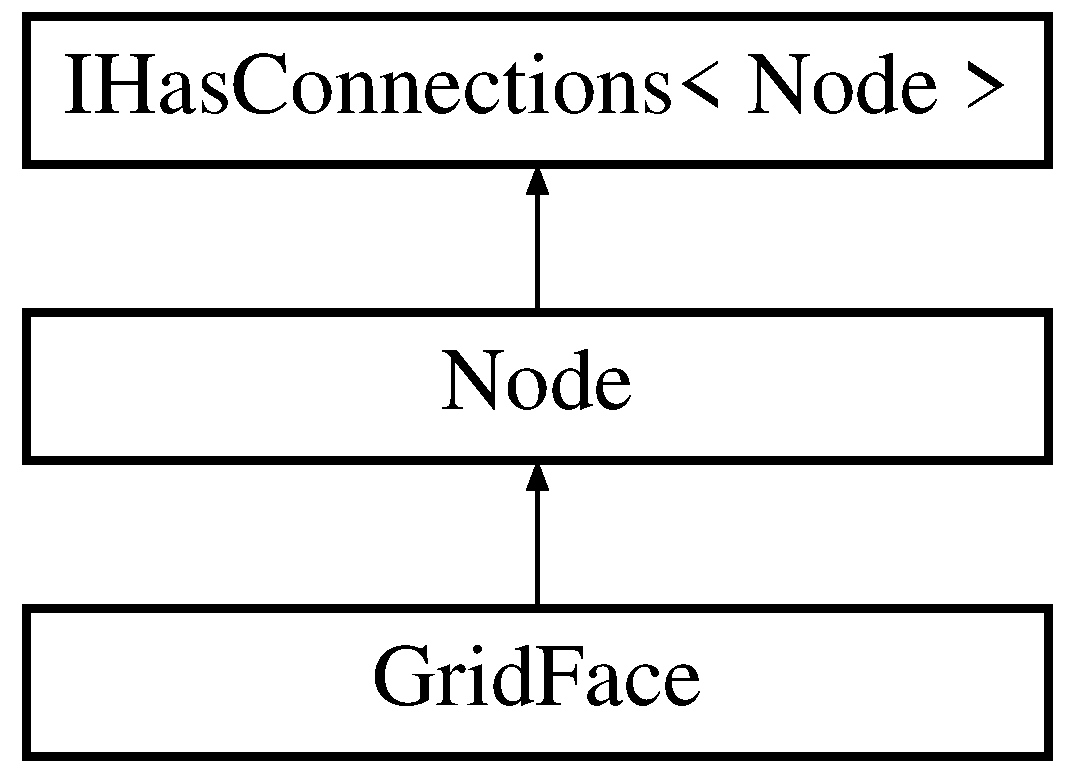
\includegraphics[height=3.000000cm]{class_grid_face}
\end{center}
\end{figure}
\subsection*{Public Member Functions}
\begin{DoxyCompactItemize}
\item 
\mbox{\hyperlink{class_grid_face_a328917a6e83b3357fbb95aae6c43b861}{Grid\+Face}} ()
\item 
\mbox{\hyperlink{class_grid_face_a2f31cf59941dd0886b1a9a3bd3eec590}{Grid\+Face}} (Vector2 position2)
\item 
\mbox{\hyperlink{class_grid_face_adb30d4c2fb9f5be07319720fb21481ba}{Grid\+Face}} (Vector3 \mbox{\hyperlink{class_node_a315059cd3874b8ca61426a4e1bd097a7}{position}})
\item 
void \mbox{\hyperlink{class_grid_face_a55db6fc7a977c60fd6ce94de473d895c}{Add\+Vertices}} (\mbox{\hyperlink{class_node}{Node}}\mbox{[}$\,$\mbox{]} \mbox{\hyperlink{class_grid_face_ad283473ab08b56840f9ae843e60c1d15}{vertices}})
\item 
int \mbox{\hyperlink{class_grid_face_af0f04e74e12e9ee8f03a6675ee5a4eab}{Add\+Vertex}} (\mbox{\hyperlink{class_node}{Node}} vertex)
\item 
int \mbox{\hyperlink{class_grid_face_a31c9530fd0dca84658fde5ddfc369fc5}{Num\+Vertices}} ()
\item 
\mbox{\hyperlink{class_node}{Node}} \mbox{\hyperlink{class_grid_face_a153928011211a1740054bf60adf67730}{Get\+Vertex}} (int index)
\item 
bool \mbox{\hyperlink{class_grid_face_ad038c4fab1850cb71cdb8b4a0c2f52f2}{Has\+Vertex}} (\mbox{\hyperlink{class_node}{Node}} vertex)
\item 
\mbox{\hyperlink{class_node}{Node}} \mbox{\hyperlink{class_grid_face_a19159b9927ce52f293e566975fcd3340}{Get\+Connection\+With\+Vertex}} (\mbox{\hyperlink{class_node}{Node}} vertex)
\item 
List$<$ Vector3 $>$ \mbox{\hyperlink{class_grid_face_af4dabd4122b97fca940b763ca0000100}{Get\+Vertex\+Positions}} ()
\item 
\mbox{\hyperlink{class_node}{Node}} \mbox{[}$\,$\mbox{]} \mbox{\hyperlink{class_grid_face_a60aa8f74afb2447bf1921385581c8972}{Get\+Vertices}} ()
\end{DoxyCompactItemize}
\subsection*{Protected Member Functions}
\begin{DoxyCompactItemize}
\item 
int \mbox{\hyperlink{class_grid_face_a4a97d1968f8e31252c109c6a817d4db5}{Find\+Connection\+With\+Vertex}} (\mbox{\hyperlink{class_node}{Node}} vertex)
\item 
void \mbox{\hyperlink{class_grid_face_a7a09019689547ed0d1e719f999e9a50b}{Swap\+Vertices}} (int i, int j)
\end{DoxyCompactItemize}
\subsection*{Protected Attributes}
\begin{DoxyCompactItemize}
\item 
List$<$ \mbox{\hyperlink{class_node}{Node}} $>$ \mbox{\hyperlink{class_grid_face_ad283473ab08b56840f9ae843e60c1d15}{vertices}}
\end{DoxyCompactItemize}


\subsection{Constructor \& Destructor Documentation}
\mbox{\Hypertarget{class_grid_face_a328917a6e83b3357fbb95aae6c43b861}\label{class_grid_face_a328917a6e83b3357fbb95aae6c43b861}} 
\index{Grid\+Face@{Grid\+Face}!Grid\+Face@{Grid\+Face}}
\index{Grid\+Face@{Grid\+Face}!Grid\+Face@{Grid\+Face}}
\subsubsection{\texorpdfstring{Grid\+Face()}{GridFace()}\hspace{0.1cm}{\footnotesize\ttfamily [1/3]}}
{\footnotesize\ttfamily Grid\+Face.\+Grid\+Face (\begin{DoxyParamCaption}{ }\end{DoxyParamCaption})}

\mbox{\Hypertarget{class_grid_face_a2f31cf59941dd0886b1a9a3bd3eec590}\label{class_grid_face_a2f31cf59941dd0886b1a9a3bd3eec590}} 
\index{Grid\+Face@{Grid\+Face}!Grid\+Face@{Grid\+Face}}
\index{Grid\+Face@{Grid\+Face}!Grid\+Face@{Grid\+Face}}
\subsubsection{\texorpdfstring{Grid\+Face()}{GridFace()}\hspace{0.1cm}{\footnotesize\ttfamily [2/3]}}
{\footnotesize\ttfamily Grid\+Face.\+Grid\+Face (\begin{DoxyParamCaption}\item[{Vector2}]{position2 }\end{DoxyParamCaption})}

\mbox{\Hypertarget{class_grid_face_adb30d4c2fb9f5be07319720fb21481ba}\label{class_grid_face_adb30d4c2fb9f5be07319720fb21481ba}} 
\index{Grid\+Face@{Grid\+Face}!Grid\+Face@{Grid\+Face}}
\index{Grid\+Face@{Grid\+Face}!Grid\+Face@{Grid\+Face}}
\subsubsection{\texorpdfstring{Grid\+Face()}{GridFace()}\hspace{0.1cm}{\footnotesize\ttfamily [3/3]}}
{\footnotesize\ttfamily Grid\+Face.\+Grid\+Face (\begin{DoxyParamCaption}\item[{Vector3}]{position }\end{DoxyParamCaption})}



\subsection{Member Function Documentation}
\mbox{\Hypertarget{class_grid_face_af0f04e74e12e9ee8f03a6675ee5a4eab}\label{class_grid_face_af0f04e74e12e9ee8f03a6675ee5a4eab}} 
\index{Grid\+Face@{Grid\+Face}!Add\+Vertex@{Add\+Vertex}}
\index{Add\+Vertex@{Add\+Vertex}!Grid\+Face@{Grid\+Face}}
\subsubsection{\texorpdfstring{Add\+Vertex()}{AddVertex()}}
{\footnotesize\ttfamily int Grid\+Face.\+Add\+Vertex (\begin{DoxyParamCaption}\item[{\mbox{\hyperlink{class_node}{Node}}}]{vertex }\end{DoxyParamCaption})}

\mbox{\Hypertarget{class_grid_face_a55db6fc7a977c60fd6ce94de473d895c}\label{class_grid_face_a55db6fc7a977c60fd6ce94de473d895c}} 
\index{Grid\+Face@{Grid\+Face}!Add\+Vertices@{Add\+Vertices}}
\index{Add\+Vertices@{Add\+Vertices}!Grid\+Face@{Grid\+Face}}
\subsubsection{\texorpdfstring{Add\+Vertices()}{AddVertices()}}
{\footnotesize\ttfamily void Grid\+Face.\+Add\+Vertices (\begin{DoxyParamCaption}\item[{\mbox{\hyperlink{class_node}{Node}} \mbox{[}$\,$\mbox{]}}]{vertices }\end{DoxyParamCaption})}

\mbox{\Hypertarget{class_grid_face_a4a97d1968f8e31252c109c6a817d4db5}\label{class_grid_face_a4a97d1968f8e31252c109c6a817d4db5}} 
\index{Grid\+Face@{Grid\+Face}!Find\+Connection\+With\+Vertex@{Find\+Connection\+With\+Vertex}}
\index{Find\+Connection\+With\+Vertex@{Find\+Connection\+With\+Vertex}!Grid\+Face@{Grid\+Face}}
\subsubsection{\texorpdfstring{Find\+Connection\+With\+Vertex()}{FindConnectionWithVertex()}}
{\footnotesize\ttfamily int Grid\+Face.\+Find\+Connection\+With\+Vertex (\begin{DoxyParamCaption}\item[{\mbox{\hyperlink{class_node}{Node}}}]{vertex }\end{DoxyParamCaption})\hspace{0.3cm}{\ttfamily [protected]}}

\mbox{\Hypertarget{class_grid_face_a19159b9927ce52f293e566975fcd3340}\label{class_grid_face_a19159b9927ce52f293e566975fcd3340}} 
\index{Grid\+Face@{Grid\+Face}!Get\+Connection\+With\+Vertex@{Get\+Connection\+With\+Vertex}}
\index{Get\+Connection\+With\+Vertex@{Get\+Connection\+With\+Vertex}!Grid\+Face@{Grid\+Face}}
\subsubsection{\texorpdfstring{Get\+Connection\+With\+Vertex()}{GetConnectionWithVertex()}}
{\footnotesize\ttfamily \mbox{\hyperlink{class_node}{Node}} Grid\+Face.\+Get\+Connection\+With\+Vertex (\begin{DoxyParamCaption}\item[{\mbox{\hyperlink{class_node}{Node}}}]{vertex }\end{DoxyParamCaption})}

\mbox{\Hypertarget{class_grid_face_a153928011211a1740054bf60adf67730}\label{class_grid_face_a153928011211a1740054bf60adf67730}} 
\index{Grid\+Face@{Grid\+Face}!Get\+Vertex@{Get\+Vertex}}
\index{Get\+Vertex@{Get\+Vertex}!Grid\+Face@{Grid\+Face}}
\subsubsection{\texorpdfstring{Get\+Vertex()}{GetVertex()}}
{\footnotesize\ttfamily \mbox{\hyperlink{class_node}{Node}} Grid\+Face.\+Get\+Vertex (\begin{DoxyParamCaption}\item[{int}]{index }\end{DoxyParamCaption})}

\mbox{\Hypertarget{class_grid_face_af4dabd4122b97fca940b763ca0000100}\label{class_grid_face_af4dabd4122b97fca940b763ca0000100}} 
\index{Grid\+Face@{Grid\+Face}!Get\+Vertex\+Positions@{Get\+Vertex\+Positions}}
\index{Get\+Vertex\+Positions@{Get\+Vertex\+Positions}!Grid\+Face@{Grid\+Face}}
\subsubsection{\texorpdfstring{Get\+Vertex\+Positions()}{GetVertexPositions()}}
{\footnotesize\ttfamily List$<$Vector3$>$ Grid\+Face.\+Get\+Vertex\+Positions (\begin{DoxyParamCaption}{ }\end{DoxyParamCaption})}

\mbox{\Hypertarget{class_grid_face_a60aa8f74afb2447bf1921385581c8972}\label{class_grid_face_a60aa8f74afb2447bf1921385581c8972}} 
\index{Grid\+Face@{Grid\+Face}!Get\+Vertices@{Get\+Vertices}}
\index{Get\+Vertices@{Get\+Vertices}!Grid\+Face@{Grid\+Face}}
\subsubsection{\texorpdfstring{Get\+Vertices()}{GetVertices()}}
{\footnotesize\ttfamily \mbox{\hyperlink{class_node}{Node}} \mbox{[}$\,$\mbox{]} Grid\+Face.\+Get\+Vertices (\begin{DoxyParamCaption}{ }\end{DoxyParamCaption})}

\mbox{\Hypertarget{class_grid_face_ad038c4fab1850cb71cdb8b4a0c2f52f2}\label{class_grid_face_ad038c4fab1850cb71cdb8b4a0c2f52f2}} 
\index{Grid\+Face@{Grid\+Face}!Has\+Vertex@{Has\+Vertex}}
\index{Has\+Vertex@{Has\+Vertex}!Grid\+Face@{Grid\+Face}}
\subsubsection{\texorpdfstring{Has\+Vertex()}{HasVertex()}}
{\footnotesize\ttfamily bool Grid\+Face.\+Has\+Vertex (\begin{DoxyParamCaption}\item[{\mbox{\hyperlink{class_node}{Node}}}]{vertex }\end{DoxyParamCaption})}

\mbox{\Hypertarget{class_grid_face_a31c9530fd0dca84658fde5ddfc369fc5}\label{class_grid_face_a31c9530fd0dca84658fde5ddfc369fc5}} 
\index{Grid\+Face@{Grid\+Face}!Num\+Vertices@{Num\+Vertices}}
\index{Num\+Vertices@{Num\+Vertices}!Grid\+Face@{Grid\+Face}}
\subsubsection{\texorpdfstring{Num\+Vertices()}{NumVertices()}}
{\footnotesize\ttfamily int Grid\+Face.\+Num\+Vertices (\begin{DoxyParamCaption}{ }\end{DoxyParamCaption})}

\mbox{\Hypertarget{class_grid_face_a7a09019689547ed0d1e719f999e9a50b}\label{class_grid_face_a7a09019689547ed0d1e719f999e9a50b}} 
\index{Grid\+Face@{Grid\+Face}!Swap\+Vertices@{Swap\+Vertices}}
\index{Swap\+Vertices@{Swap\+Vertices}!Grid\+Face@{Grid\+Face}}
\subsubsection{\texorpdfstring{Swap\+Vertices()}{SwapVertices()}}
{\footnotesize\ttfamily void Grid\+Face.\+Swap\+Vertices (\begin{DoxyParamCaption}\item[{int}]{i,  }\item[{int}]{j }\end{DoxyParamCaption})\hspace{0.3cm}{\ttfamily [protected]}}



\subsection{Member Data Documentation}
\mbox{\Hypertarget{class_grid_face_ad283473ab08b56840f9ae843e60c1d15}\label{class_grid_face_ad283473ab08b56840f9ae843e60c1d15}} 
\index{Grid\+Face@{Grid\+Face}!vertices@{vertices}}
\index{vertices@{vertices}!Grid\+Face@{Grid\+Face}}
\subsubsection{\texorpdfstring{vertices}{vertices}}
{\footnotesize\ttfamily List$<$\mbox{\hyperlink{class_node}{Node}}$>$ Grid\+Face.\+vertices\hspace{0.3cm}{\ttfamily [protected]}}



The documentation for this class was generated from the following file\+:\begin{DoxyCompactItemize}
\item 
/\+Users/sabienambrose/\+Documents/\+Coding/\+Unity\+Mechanical\+Turk/\+Mechanical\+Turk/\+Assets/\+Scripts/\+Util/\+Containers/\+Graphs/\+Grids/\mbox{\hyperlink{_grid_face_8cs}{Grid\+Face.\+cs}}\end{DoxyCompactItemize}

\hypertarget{class_grid_factory}{}\section{Grid\+Factory Class Reference}
\label{class_grid_factory}\index{Grid\+Factory@{Grid\+Factory}}
\subsection*{Static Public Member Functions}
\begin{DoxyCompactItemize}
\item 
static bool \mbox{\hyperlink{class_grid_factory_ae31ccb1316ff0273b63f3d9b099be036}{Create\+Square\+Grid}} (\mbox{\hyperlink{struct_square_grid_params}{Square\+Grid\+Params}} grid\+Params, out \mbox{\hyperlink{class_poly_grid}{Poly\+Grid}} grid)
\item 
static bool \mbox{\hyperlink{class_grid_factory_a4878217f8fa48b3ed205e9b4a6e863e2}{Populate\+Square\+Grid}} (ref \mbox{\hyperlink{class_poly_grid}{Poly\+Grid}} grid)
\end{DoxyCompactItemize}


\subsection{Member Function Documentation}
\mbox{\Hypertarget{class_grid_factory_ae31ccb1316ff0273b63f3d9b099be036}\label{class_grid_factory_ae31ccb1316ff0273b63f3d9b099be036}} 
\index{Grid\+Factory@{Grid\+Factory}!Create\+Square\+Grid@{Create\+Square\+Grid}}
\index{Create\+Square\+Grid@{Create\+Square\+Grid}!Grid\+Factory@{Grid\+Factory}}
\subsubsection{\texorpdfstring{Create\+Square\+Grid()}{CreateSquareGrid()}}
{\footnotesize\ttfamily static bool Grid\+Factory.\+Create\+Square\+Grid (\begin{DoxyParamCaption}\item[{\mbox{\hyperlink{struct_square_grid_params}{Square\+Grid\+Params}}}]{grid\+Params,  }\item[{out \mbox{\hyperlink{class_poly_grid}{Poly\+Grid}}}]{grid }\end{DoxyParamCaption})\hspace{0.3cm}{\ttfamily [static]}}

\mbox{\Hypertarget{class_grid_factory_a4878217f8fa48b3ed205e9b4a6e863e2}\label{class_grid_factory_a4878217f8fa48b3ed205e9b4a6e863e2}} 
\index{Grid\+Factory@{Grid\+Factory}!Populate\+Square\+Grid@{Populate\+Square\+Grid}}
\index{Populate\+Square\+Grid@{Populate\+Square\+Grid}!Grid\+Factory@{Grid\+Factory}}
\subsubsection{\texorpdfstring{Populate\+Square\+Grid()}{PopulateSquareGrid()}}
{\footnotesize\ttfamily static bool Grid\+Factory.\+Populate\+Square\+Grid (\begin{DoxyParamCaption}\item[{ref \mbox{\hyperlink{class_poly_grid}{Poly\+Grid}}}]{grid }\end{DoxyParamCaption})\hspace{0.3cm}{\ttfamily [static]}}



The documentation for this class was generated from the following file\+:\begin{DoxyCompactItemize}
\item 
/\+Users/sabienambrose/\+Documents/\+Coding/\+Unity\+Mechanical\+Turk/\+Mechanical\+Turk/\+Assets/\+Scripts/\+Util/\+Containers/\+Graphs/\+Grids/\mbox{\hyperlink{_grid_factory_8cs}{Grid\+Factory.\+cs}}\end{DoxyCompactItemize}

\hypertarget{class_heuristic}{}\section{Heuristic$<$ T $>$ Class Template Reference}
\label{class_heuristic}\index{Heuristic$<$ T $>$@{Heuristic$<$ T $>$}}
Inheritance diagram for Heuristic$<$ T $>$\+:\begin{figure}[H]
\begin{center}
\leavevmode
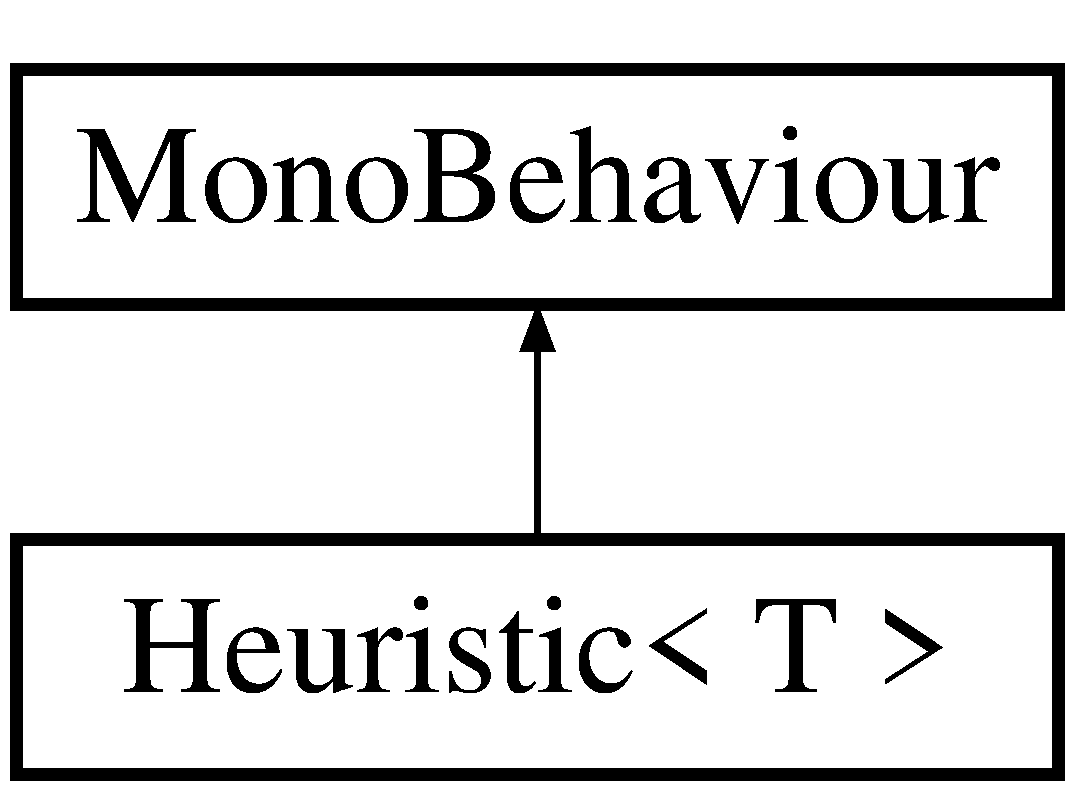
\includegraphics[height=2.000000cm]{class_heuristic}
\end{center}
\end{figure}
\subsection*{Public Member Functions}
\begin{DoxyCompactItemize}
\item 
virtual float \mbox{\hyperlink{class_heuristic_a89a45e2edf451260032d107d6118ac04}{Estimate}} (T node)
\end{DoxyCompactItemize}
\subsection*{Public Attributes}
\begin{DoxyCompactItemize}
\item 
T \mbox{\hyperlink{class_heuristic_a9b7078c615bf30ac77f026a737d6169a}{goal}}
\end{DoxyCompactItemize}


\subsection{Member Function Documentation}
\mbox{\Hypertarget{class_heuristic_a89a45e2edf451260032d107d6118ac04}\label{class_heuristic_a89a45e2edf451260032d107d6118ac04}} 
\index{Heuristic@{Heuristic}!Estimate@{Estimate}}
\index{Estimate@{Estimate}!Heuristic@{Heuristic}}
\subsubsection{\texorpdfstring{Estimate()}{Estimate()}}
{\footnotesize\ttfamily virtual float \mbox{\hyperlink{class_heuristic}{Heuristic}}$<$ T $>$.Estimate (\begin{DoxyParamCaption}\item[{T}]{node }\end{DoxyParamCaption})\hspace{0.3cm}{\ttfamily [virtual]}}



\subsection{Member Data Documentation}
\mbox{\Hypertarget{class_heuristic_a9b7078c615bf30ac77f026a737d6169a}\label{class_heuristic_a9b7078c615bf30ac77f026a737d6169a}} 
\index{Heuristic@{Heuristic}!goal@{goal}}
\index{goal@{goal}!Heuristic@{Heuristic}}
\subsubsection{\texorpdfstring{goal}{goal}}
{\footnotesize\ttfamily T \mbox{\hyperlink{class_heuristic}{Heuristic}}$<$ T $>$.goal}



The documentation for this class was generated from the following file\+:\begin{DoxyCompactItemize}
\item 
/\+Users/sabienambrose/\+Documents/\+Coding/\+Unity\+Mechanical\+Turk/\+Mechanical\+Turk/\+Assets/\+Scripts/\+Pathfinding/\+Heuristics/\mbox{\hyperlink{_heuristic_8cs}{Heuristic.\+cs}}\end{DoxyCompactItemize}

\hypertarget{interface_i_connection}{}\section{I\+Connection$<$ T $>$ Interface Template Reference}
\label{interface_i_connection}\index{I\+Connection$<$ T $>$@{I\+Connection$<$ T $>$}}
Inheritance diagram for I\+Connection$<$ T $>$\+:\begin{figure}[H]
\begin{center}
\leavevmode
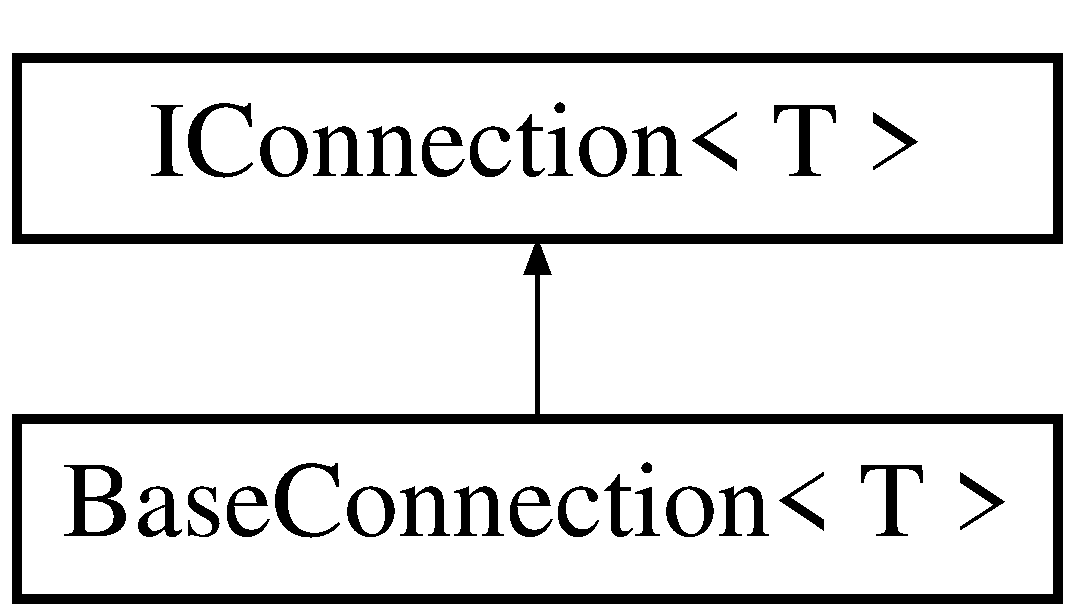
\includegraphics[height=2.000000cm]{interface_i_connection}
\end{center}
\end{figure}
\subsection*{Public Member Functions}
\begin{DoxyCompactItemize}
\item 
float \mbox{\hyperlink{interface_i_connection_adf42d8cf17bee3b3b1ee299d6f9de1df}{Get\+Cost}} ()
\begin{DoxyCompactList}\small\item\em Returns the non-\/negative cost of the connection \end{DoxyCompactList}\item 
T \mbox{\hyperlink{interface_i_connection_acecfce42b26af8f2f83e3a806edc6910}{Get\+From\+Node}} ()
\begin{DoxyCompactList}\small\item\em Returns the id of the node that this connection from. \end{DoxyCompactList}\item 
T \mbox{\hyperlink{interface_i_connection_a738b6e5b2c2620e9e4a8a3e07fe85b52}{Get\+To\+Node}} ()
\begin{DoxyCompactList}\small\item\em Returns the id of the node that this connection leads to. \end{DoxyCompactList}\item 
bool \mbox{\hyperlink{interface_i_connection_a0789fc3877953a8da47402b986c8469d}{Has\+Node}} (T t)
\end{DoxyCompactItemize}


\subsection{Member Function Documentation}
\mbox{\Hypertarget{interface_i_connection_adf42d8cf17bee3b3b1ee299d6f9de1df}\label{interface_i_connection_adf42d8cf17bee3b3b1ee299d6f9de1df}} 
\index{I\+Connection@{I\+Connection}!Get\+Cost@{Get\+Cost}}
\index{Get\+Cost@{Get\+Cost}!I\+Connection@{I\+Connection}}
\subsubsection{\texorpdfstring{Get\+Cost()}{GetCost()}}
{\footnotesize\ttfamily float \mbox{\hyperlink{interface_i_connection}{I\+Connection}}$<$ T $>$.Get\+Cost (\begin{DoxyParamCaption}{ }\end{DoxyParamCaption})}



Returns the non-\/negative cost of the connection 

\begin{DoxyReturn}{Returns}

\end{DoxyReturn}


Implemented in \mbox{\hyperlink{class_base_connection_a3f2351e9bf997450cca8f64e1e32337a}{Base\+Connection$<$ T $>$}}.

\mbox{\Hypertarget{interface_i_connection_acecfce42b26af8f2f83e3a806edc6910}\label{interface_i_connection_acecfce42b26af8f2f83e3a806edc6910}} 
\index{I\+Connection@{I\+Connection}!Get\+From\+Node@{Get\+From\+Node}}
\index{Get\+From\+Node@{Get\+From\+Node}!I\+Connection@{I\+Connection}}
\subsubsection{\texorpdfstring{Get\+From\+Node()}{GetFromNode()}}
{\footnotesize\ttfamily T \mbox{\hyperlink{interface_i_connection}{I\+Connection}}$<$ T $>$.Get\+From\+Node (\begin{DoxyParamCaption}{ }\end{DoxyParamCaption})}



Returns the id of the node that this connection from. 

\begin{DoxyReturn}{Returns}

\end{DoxyReturn}


Implemented in \mbox{\hyperlink{class_base_connection_a45f52b2a297e6ac3a1bca5b5b0d80b89}{Base\+Connection$<$ T $>$}}.

\mbox{\Hypertarget{interface_i_connection_a738b6e5b2c2620e9e4a8a3e07fe85b52}\label{interface_i_connection_a738b6e5b2c2620e9e4a8a3e07fe85b52}} 
\index{I\+Connection@{I\+Connection}!Get\+To\+Node@{Get\+To\+Node}}
\index{Get\+To\+Node@{Get\+To\+Node}!I\+Connection@{I\+Connection}}
\subsubsection{\texorpdfstring{Get\+To\+Node()}{GetToNode()}}
{\footnotesize\ttfamily T \mbox{\hyperlink{interface_i_connection}{I\+Connection}}$<$ T $>$.Get\+To\+Node (\begin{DoxyParamCaption}{ }\end{DoxyParamCaption})}



Returns the id of the node that this connection leads to. 

\begin{DoxyReturn}{Returns}

\end{DoxyReturn}


Implemented in \mbox{\hyperlink{class_base_connection_ad6baf1f89a5abd5f860e1ec58244aab7}{Base\+Connection$<$ T $>$}}.

\mbox{\Hypertarget{interface_i_connection_a0789fc3877953a8da47402b986c8469d}\label{interface_i_connection_a0789fc3877953a8da47402b986c8469d}} 
\index{I\+Connection@{I\+Connection}!Has\+Node@{Has\+Node}}
\index{Has\+Node@{Has\+Node}!I\+Connection@{I\+Connection}}
\subsubsection{\texorpdfstring{Has\+Node()}{HasNode()}}
{\footnotesize\ttfamily bool \mbox{\hyperlink{interface_i_connection}{I\+Connection}}$<$ T $>$.Has\+Node (\begin{DoxyParamCaption}\item[{T}]{t }\end{DoxyParamCaption})}



Implemented in \mbox{\hyperlink{class_base_connection_a94d80620b77e0c9c0afdcef31ade9196}{Base\+Connection$<$ T $>$}}.



The documentation for this interface was generated from the following file\+:\begin{DoxyCompactItemize}
\item 
/\+Users/sabienambrose/\+Documents/\+Coding/\+Unity\+Mechanical\+Turk/\+Mechanical\+Turk/\+Assets/\+Scripts/\+Util/\+Containers/\+Graphs/\mbox{\hyperlink{_graph_types_8cs}{Graph\+Types.\+cs}}\end{DoxyCompactItemize}

\hypertarget{interface_i_graph}{}\section{I\+Graph$<$ T $>$ Interface Template Reference}
\label{interface_i_graph}\index{I\+Graph$<$ T $>$@{I\+Graph$<$ T $>$}}
\subsection*{Public Member Functions}
\begin{DoxyCompactItemize}
\item 
void \mbox{\hyperlink{interface_i_graph_ac0a171fdc636178c7dbbaaf830d7d15a}{Get\+Connections}} (T from\+Node, out List$<$ \mbox{\hyperlink{interface_i_connection}{I\+Connection}}$<$ T $>$$>$ connections)
\begin{DoxyCompactList}\small\item\em Returns an array of connections (implementing \mbox{\hyperlink{interface_i_connection}{I\+Connection}}) outgoing from the given node. \end{DoxyCompactList}\end{DoxyCompactItemize}


\subsection{Member Function Documentation}
\mbox{\Hypertarget{interface_i_graph_ac0a171fdc636178c7dbbaaf830d7d15a}\label{interface_i_graph_ac0a171fdc636178c7dbbaaf830d7d15a}} 
\index{I\+Graph@{I\+Graph}!Get\+Connections@{Get\+Connections}}
\index{Get\+Connections@{Get\+Connections}!I\+Graph@{I\+Graph}}
\subsubsection{\texorpdfstring{Get\+Connections()}{GetConnections()}}
{\footnotesize\ttfamily void \mbox{\hyperlink{interface_i_graph}{I\+Graph}}$<$ T $>$.Get\+Connections (\begin{DoxyParamCaption}\item[{T}]{from\+Node,  }\item[{out List$<$ \mbox{\hyperlink{interface_i_connection}{I\+Connection}}$<$ T $>$$>$}]{connections }\end{DoxyParamCaption})}



Returns an array of connections (implementing \mbox{\hyperlink{interface_i_connection}{I\+Connection}}) outgoing from the given node. 


\begin{DoxyParams}{Parameters}
{\em from\+Node} & The node whose connections to return.\\
\hline
{\em connections} & The connections to return.\\
\hline
\end{DoxyParams}


The documentation for this interface was generated from the following file\+:\begin{DoxyCompactItemize}
\item 
/\+Users/sabienambrose/\+Documents/\+Coding/\+Unity\+Mechanical\+Turk/\+Mechanical\+Turk/\+Assets/\+Scripts/\+Util/\+Containers/\+Graphs/\mbox{\hyperlink{_graph_types_8cs}{Graph\+Types.\+cs}}\end{DoxyCompactItemize}

\hypertarget{interface_i_has_connections}{}\section{I\+Has\+Connections$<$ T $>$ Interface Template Reference}
\label{interface_i_has_connections}\index{I\+Has\+Connections$<$ T $>$@{I\+Has\+Connections$<$ T $>$}}
\subsection*{Public Member Functions}
\begin{DoxyCompactItemize}
\item 
void \mbox{\hyperlink{interface_i_has_connections_a10802404b8cf026d9755ef3c2c9ce075}{Get\+Connections}} (out List$<$ \mbox{\hyperlink{interface_i_connection}{I\+Connection}}$<$ T $>$$>$ connections)
\begin{DoxyCompactList}\small\item\em Returns an array of connections (implementing \mbox{\hyperlink{interface_i_connection}{I\+Connection}}) outgoing from self \end{DoxyCompactList}\item 
bool \mbox{\hyperlink{interface_i_has_connections_aaf582ecd5ed3d37d6a69b94fb947d9cb}{Is\+Connected\+To}} (T other)
\end{DoxyCompactItemize}


\subsection{Member Function Documentation}
\mbox{\Hypertarget{interface_i_has_connections_a10802404b8cf026d9755ef3c2c9ce075}\label{interface_i_has_connections_a10802404b8cf026d9755ef3c2c9ce075}} 
\index{I\+Has\+Connections@{I\+Has\+Connections}!Get\+Connections@{Get\+Connections}}
\index{Get\+Connections@{Get\+Connections}!I\+Has\+Connections@{I\+Has\+Connections}}
\subsubsection{\texorpdfstring{Get\+Connections()}{GetConnections()}}
{\footnotesize\ttfamily void \mbox{\hyperlink{interface_i_has_connections}{I\+Has\+Connections}}$<$ T $>$.Get\+Connections (\begin{DoxyParamCaption}\item[{out List$<$ \mbox{\hyperlink{interface_i_connection}{I\+Connection}}$<$ T $>$$>$}]{connections }\end{DoxyParamCaption})}



Returns an array of connections (implementing \mbox{\hyperlink{interface_i_connection}{I\+Connection}}) outgoing from self 


\begin{DoxyParams}{Parameters}
{\em connections} & The connections to return.\\
\hline
\end{DoxyParams}
\mbox{\Hypertarget{interface_i_has_connections_aaf582ecd5ed3d37d6a69b94fb947d9cb}\label{interface_i_has_connections_aaf582ecd5ed3d37d6a69b94fb947d9cb}} 
\index{I\+Has\+Connections@{I\+Has\+Connections}!Is\+Connected\+To@{Is\+Connected\+To}}
\index{Is\+Connected\+To@{Is\+Connected\+To}!I\+Has\+Connections@{I\+Has\+Connections}}
\subsubsection{\texorpdfstring{Is\+Connected\+To()}{IsConnectedTo()}}
{\footnotesize\ttfamily bool \mbox{\hyperlink{interface_i_has_connections}{I\+Has\+Connections}}$<$ T $>$.Is\+Connected\+To (\begin{DoxyParamCaption}\item[{T}]{other }\end{DoxyParamCaption})}



The documentation for this interface was generated from the following file\+:\begin{DoxyCompactItemize}
\item 
/\+Users/sabienambrose/\+Documents/\+Coding/\+Unity\+Mechanical\+Turk/\+Mechanical\+Turk/\+Assets/\+Scripts/\+Util/\+Containers/\+Graphs/\mbox{\hyperlink{_graph_types_8cs}{Graph\+Types.\+cs}}\end{DoxyCompactItemize}

\hypertarget{struct_int_point}{}\section{Int\+Point Struct Reference}
\label{struct_int_point}\index{Int\+Point@{Int\+Point}}
\subsection*{Public Member Functions}
\begin{DoxyCompactItemize}
\item 
\mbox{\hyperlink{struct_int_point_a553ad71275bc778ad20bda98cb3b760c}{Int\+Point}} (int \mbox{\hyperlink{struct_int_point_a939365b5f010e65361371b8ee69c2080}{x}}, int \mbox{\hyperlink{struct_int_point_ac7e0bbc435a90aac2c4136ec83e3f3ef}{y}})
\item 
\mbox{\hyperlink{struct_int_point_a89c7250ab8d007dfc10123d4eb5a32ca}{Int\+Point}} (float \mbox{\hyperlink{struct_int_point_a939365b5f010e65361371b8ee69c2080}{x}}, float \mbox{\hyperlink{struct_int_point_ac7e0bbc435a90aac2c4136ec83e3f3ef}{y}})
\item 
\mbox{\hyperlink{struct_int_point_ab12389b14a95036d62ab7449458b0da1}{Int\+Point}} (Vector2 v)
\item 
Vector2 \mbox{\hyperlink{struct_int_point_a755fe840cba345e23b9adba59c954ee1}{To\+Vector}} ()
\item 
override string \mbox{\hyperlink{struct_int_point_a1d4d1b0f6bdabf751d65167bd9c257c8}{To\+String}} ()
\item 
override bool \mbox{\hyperlink{struct_int_point_af2fa9d4fae137e551b3365cacbad2cdc}{Equals}} (object obj)
\item 
bool \mbox{\hyperlink{struct_int_point_a4164fdfc1ff4c090ac281503b12a447c}{Greater\+Than}} (\mbox{\hyperlink{struct_int_point}{Int\+Point}} p)
\item 
bool \mbox{\hyperlink{struct_int_point_a8a4396b524a0872981a7a7505b19bde7}{Less\+Than}} (\mbox{\hyperlink{struct_int_point}{Int\+Point}} p)
\end{DoxyCompactItemize}
\subsection*{Static Public Member Functions}
\begin{DoxyCompactItemize}
\item 
static \mbox{\hyperlink{struct_int_point}{Int\+Point}} \mbox{\hyperlink{struct_int_point_ad3c6094ef41ce5eb1717aba101160c94}{Zero}} ()
\item 
static \mbox{\hyperlink{struct_int_point}{Int\+Point}} \mbox{\hyperlink{struct_int_point_a241b96189209f3c2036424091a910909}{Add}} (\mbox{\hyperlink{struct_int_point}{Int\+Point}} a, \mbox{\hyperlink{struct_int_point}{Int\+Point}} b)
\item 
static \mbox{\hyperlink{struct_int_point}{Int\+Point}} \mbox{\hyperlink{struct_int_point_a4f467361e4cd5eebddeddcb9f6b8ffa4}{Add}} (\mbox{\hyperlink{struct_int_point}{Int\+Point}} a, int \mbox{\hyperlink{struct_int_point_a939365b5f010e65361371b8ee69c2080}{x}}, int \mbox{\hyperlink{struct_int_point_ac7e0bbc435a90aac2c4136ec83e3f3ef}{y}})
\item 
static \mbox{\hyperlink{struct_int_point}{Int\+Point}} \mbox{\hyperlink{struct_int_point_ab9a48f33c1886477e13049121e16a070}{Sub}} (\mbox{\hyperlink{struct_int_point}{Int\+Point}} a, int \mbox{\hyperlink{struct_int_point_a939365b5f010e65361371b8ee69c2080}{x}}, int \mbox{\hyperlink{struct_int_point_ac7e0bbc435a90aac2c4136ec83e3f3ef}{y}})
\item 
static \mbox{\hyperlink{struct_int_point}{Int\+Point}} \mbox{\hyperlink{struct_int_point_add7064e8013bc061ff7c800362c78634}{Sub}} (\mbox{\hyperlink{struct_int_point}{Int\+Point}} a, \mbox{\hyperlink{struct_int_point}{Int\+Point}} b)
\item 
static float \mbox{\hyperlink{struct_int_point_ad43affc9a7f25aa4bf680b756a3b81da}{Distance}} (\mbox{\hyperlink{struct_int_point}{Int\+Point}} a, \mbox{\hyperlink{struct_int_point}{Int\+Point}} b)
\end{DoxyCompactItemize}
\subsection*{Public Attributes}
\begin{DoxyCompactItemize}
\item 
int \mbox{\hyperlink{struct_int_point_a939365b5f010e65361371b8ee69c2080}{x}}
\item 
int \mbox{\hyperlink{struct_int_point_ac7e0bbc435a90aac2c4136ec83e3f3ef}{y}}
\end{DoxyCompactItemize}


\subsection{Constructor \& Destructor Documentation}
\mbox{\Hypertarget{struct_int_point_a553ad71275bc778ad20bda98cb3b760c}\label{struct_int_point_a553ad71275bc778ad20bda98cb3b760c}} 
\index{Int\+Point@{Int\+Point}!Int\+Point@{Int\+Point}}
\index{Int\+Point@{Int\+Point}!Int\+Point@{Int\+Point}}
\subsubsection{\texorpdfstring{Int\+Point()}{IntPoint()}\hspace{0.1cm}{\footnotesize\ttfamily [1/3]}}
{\footnotesize\ttfamily Int\+Point.\+Int\+Point (\begin{DoxyParamCaption}\item[{int}]{x,  }\item[{int}]{y }\end{DoxyParamCaption})}

\mbox{\Hypertarget{struct_int_point_a89c7250ab8d007dfc10123d4eb5a32ca}\label{struct_int_point_a89c7250ab8d007dfc10123d4eb5a32ca}} 
\index{Int\+Point@{Int\+Point}!Int\+Point@{Int\+Point}}
\index{Int\+Point@{Int\+Point}!Int\+Point@{Int\+Point}}
\subsubsection{\texorpdfstring{Int\+Point()}{IntPoint()}\hspace{0.1cm}{\footnotesize\ttfamily [2/3]}}
{\footnotesize\ttfamily Int\+Point.\+Int\+Point (\begin{DoxyParamCaption}\item[{float}]{x,  }\item[{float}]{y }\end{DoxyParamCaption})}

\mbox{\Hypertarget{struct_int_point_ab12389b14a95036d62ab7449458b0da1}\label{struct_int_point_ab12389b14a95036d62ab7449458b0da1}} 
\index{Int\+Point@{Int\+Point}!Int\+Point@{Int\+Point}}
\index{Int\+Point@{Int\+Point}!Int\+Point@{Int\+Point}}
\subsubsection{\texorpdfstring{Int\+Point()}{IntPoint()}\hspace{0.1cm}{\footnotesize\ttfamily [3/3]}}
{\footnotesize\ttfamily Int\+Point.\+Int\+Point (\begin{DoxyParamCaption}\item[{Vector2}]{v }\end{DoxyParamCaption})}



\subsection{Member Function Documentation}
\mbox{\Hypertarget{struct_int_point_a241b96189209f3c2036424091a910909}\label{struct_int_point_a241b96189209f3c2036424091a910909}} 
\index{Int\+Point@{Int\+Point}!Add@{Add}}
\index{Add@{Add}!Int\+Point@{Int\+Point}}
\subsubsection{\texorpdfstring{Add()}{Add()}\hspace{0.1cm}{\footnotesize\ttfamily [1/2]}}
{\footnotesize\ttfamily static \mbox{\hyperlink{struct_int_point}{Int\+Point}} Int\+Point.\+Add (\begin{DoxyParamCaption}\item[{\mbox{\hyperlink{struct_int_point}{Int\+Point}}}]{a,  }\item[{\mbox{\hyperlink{struct_int_point}{Int\+Point}}}]{b }\end{DoxyParamCaption})\hspace{0.3cm}{\ttfamily [static]}}

\mbox{\Hypertarget{struct_int_point_a4f467361e4cd5eebddeddcb9f6b8ffa4}\label{struct_int_point_a4f467361e4cd5eebddeddcb9f6b8ffa4}} 
\index{Int\+Point@{Int\+Point}!Add@{Add}}
\index{Add@{Add}!Int\+Point@{Int\+Point}}
\subsubsection{\texorpdfstring{Add()}{Add()}\hspace{0.1cm}{\footnotesize\ttfamily [2/2]}}
{\footnotesize\ttfamily static \mbox{\hyperlink{struct_int_point}{Int\+Point}} Int\+Point.\+Add (\begin{DoxyParamCaption}\item[{\mbox{\hyperlink{struct_int_point}{Int\+Point}}}]{a,  }\item[{int}]{x,  }\item[{int}]{y }\end{DoxyParamCaption})\hspace{0.3cm}{\ttfamily [static]}}

\mbox{\Hypertarget{struct_int_point_ad43affc9a7f25aa4bf680b756a3b81da}\label{struct_int_point_ad43affc9a7f25aa4bf680b756a3b81da}} 
\index{Int\+Point@{Int\+Point}!Distance@{Distance}}
\index{Distance@{Distance}!Int\+Point@{Int\+Point}}
\subsubsection{\texorpdfstring{Distance()}{Distance()}}
{\footnotesize\ttfamily static float Int\+Point.\+Distance (\begin{DoxyParamCaption}\item[{\mbox{\hyperlink{struct_int_point}{Int\+Point}}}]{a,  }\item[{\mbox{\hyperlink{struct_int_point}{Int\+Point}}}]{b }\end{DoxyParamCaption})\hspace{0.3cm}{\ttfamily [static]}}

\mbox{\Hypertarget{struct_int_point_af2fa9d4fae137e551b3365cacbad2cdc}\label{struct_int_point_af2fa9d4fae137e551b3365cacbad2cdc}} 
\index{Int\+Point@{Int\+Point}!Equals@{Equals}}
\index{Equals@{Equals}!Int\+Point@{Int\+Point}}
\subsubsection{\texorpdfstring{Equals()}{Equals()}}
{\footnotesize\ttfamily override bool Int\+Point.\+Equals (\begin{DoxyParamCaption}\item[{object}]{obj }\end{DoxyParamCaption})}

\mbox{\Hypertarget{struct_int_point_a4164fdfc1ff4c090ac281503b12a447c}\label{struct_int_point_a4164fdfc1ff4c090ac281503b12a447c}} 
\index{Int\+Point@{Int\+Point}!Greater\+Than@{Greater\+Than}}
\index{Greater\+Than@{Greater\+Than}!Int\+Point@{Int\+Point}}
\subsubsection{\texorpdfstring{Greater\+Than()}{GreaterThan()}}
{\footnotesize\ttfamily bool Int\+Point.\+Greater\+Than (\begin{DoxyParamCaption}\item[{\mbox{\hyperlink{struct_int_point}{Int\+Point}}}]{p }\end{DoxyParamCaption})}

\mbox{\Hypertarget{struct_int_point_a8a4396b524a0872981a7a7505b19bde7}\label{struct_int_point_a8a4396b524a0872981a7a7505b19bde7}} 
\index{Int\+Point@{Int\+Point}!Less\+Than@{Less\+Than}}
\index{Less\+Than@{Less\+Than}!Int\+Point@{Int\+Point}}
\subsubsection{\texorpdfstring{Less\+Than()}{LessThan()}}
{\footnotesize\ttfamily bool Int\+Point.\+Less\+Than (\begin{DoxyParamCaption}\item[{\mbox{\hyperlink{struct_int_point}{Int\+Point}}}]{p }\end{DoxyParamCaption})}

\mbox{\Hypertarget{struct_int_point_ab9a48f33c1886477e13049121e16a070}\label{struct_int_point_ab9a48f33c1886477e13049121e16a070}} 
\index{Int\+Point@{Int\+Point}!Sub@{Sub}}
\index{Sub@{Sub}!Int\+Point@{Int\+Point}}
\subsubsection{\texorpdfstring{Sub()}{Sub()}\hspace{0.1cm}{\footnotesize\ttfamily [1/2]}}
{\footnotesize\ttfamily static \mbox{\hyperlink{struct_int_point}{Int\+Point}} Int\+Point.\+Sub (\begin{DoxyParamCaption}\item[{\mbox{\hyperlink{struct_int_point}{Int\+Point}}}]{a,  }\item[{int}]{x,  }\item[{int}]{y }\end{DoxyParamCaption})\hspace{0.3cm}{\ttfamily [static]}}

\mbox{\Hypertarget{struct_int_point_add7064e8013bc061ff7c800362c78634}\label{struct_int_point_add7064e8013bc061ff7c800362c78634}} 
\index{Int\+Point@{Int\+Point}!Sub@{Sub}}
\index{Sub@{Sub}!Int\+Point@{Int\+Point}}
\subsubsection{\texorpdfstring{Sub()}{Sub()}\hspace{0.1cm}{\footnotesize\ttfamily [2/2]}}
{\footnotesize\ttfamily static \mbox{\hyperlink{struct_int_point}{Int\+Point}} Int\+Point.\+Sub (\begin{DoxyParamCaption}\item[{\mbox{\hyperlink{struct_int_point}{Int\+Point}}}]{a,  }\item[{\mbox{\hyperlink{struct_int_point}{Int\+Point}}}]{b }\end{DoxyParamCaption})\hspace{0.3cm}{\ttfamily [static]}}

\mbox{\Hypertarget{struct_int_point_a1d4d1b0f6bdabf751d65167bd9c257c8}\label{struct_int_point_a1d4d1b0f6bdabf751d65167bd9c257c8}} 
\index{Int\+Point@{Int\+Point}!To\+String@{To\+String}}
\index{To\+String@{To\+String}!Int\+Point@{Int\+Point}}
\subsubsection{\texorpdfstring{To\+String()}{ToString()}}
{\footnotesize\ttfamily override string Int\+Point.\+To\+String (\begin{DoxyParamCaption}{ }\end{DoxyParamCaption})}

\mbox{\Hypertarget{struct_int_point_a755fe840cba345e23b9adba59c954ee1}\label{struct_int_point_a755fe840cba345e23b9adba59c954ee1}} 
\index{Int\+Point@{Int\+Point}!To\+Vector@{To\+Vector}}
\index{To\+Vector@{To\+Vector}!Int\+Point@{Int\+Point}}
\subsubsection{\texorpdfstring{To\+Vector()}{ToVector()}}
{\footnotesize\ttfamily Vector2 Int\+Point.\+To\+Vector (\begin{DoxyParamCaption}{ }\end{DoxyParamCaption})}

\mbox{\Hypertarget{struct_int_point_ad3c6094ef41ce5eb1717aba101160c94}\label{struct_int_point_ad3c6094ef41ce5eb1717aba101160c94}} 
\index{Int\+Point@{Int\+Point}!Zero@{Zero}}
\index{Zero@{Zero}!Int\+Point@{Int\+Point}}
\subsubsection{\texorpdfstring{Zero()}{Zero()}}
{\footnotesize\ttfamily static \mbox{\hyperlink{struct_int_point}{Int\+Point}} Int\+Point.\+Zero (\begin{DoxyParamCaption}{ }\end{DoxyParamCaption})\hspace{0.3cm}{\ttfamily [static]}}



\subsection{Member Data Documentation}
\mbox{\Hypertarget{struct_int_point_a939365b5f010e65361371b8ee69c2080}\label{struct_int_point_a939365b5f010e65361371b8ee69c2080}} 
\index{Int\+Point@{Int\+Point}!x@{x}}
\index{x@{x}!Int\+Point@{Int\+Point}}
\subsubsection{\texorpdfstring{x}{x}}
{\footnotesize\ttfamily int Int\+Point.\+x}

\mbox{\Hypertarget{struct_int_point_ac7e0bbc435a90aac2c4136ec83e3f3ef}\label{struct_int_point_ac7e0bbc435a90aac2c4136ec83e3f3ef}} 
\index{Int\+Point@{Int\+Point}!y@{y}}
\index{y@{y}!Int\+Point@{Int\+Point}}
\subsubsection{\texorpdfstring{y}{y}}
{\footnotesize\ttfamily int Int\+Point.\+y}



The documentation for this struct was generated from the following file\+:\begin{DoxyCompactItemize}
\item 
/\+Users/sabienambrose/\+Documents/\+Coding/\+Unity\+Mechanical\+Turk/\+Mechanical\+Turk/\+Assets/\+Scripts/\+Util/\+Containers/\+Graphs/\mbox{\hyperlink{_graph_types_8cs}{Graph\+Types.\+cs}}\end{DoxyCompactItemize}

\hypertarget{struct_int_triangle}{}\section{Int\+Triangle Struct Reference}
\label{struct_int_triangle}\index{Int\+Triangle@{Int\+Triangle}}
\subsection*{Public Member Functions}
\begin{DoxyCompactItemize}
\item 
\mbox{\hyperlink{struct_int_triangle_abc1bce82e6902934849a0ba922c51a69}{Int\+Triangle}} (int \mbox{\hyperlink{struct_int_triangle_ac469d79ae7703c1bb7b3620b955da00b}{A}}, int \mbox{\hyperlink{struct_int_triangle_a643dc502fac6003f4c76a6c0a983f2dc}{B}}, int \mbox{\hyperlink{struct_int_triangle_a703a8799b3d2ed91c6fd444d028efa3a}{C}})
\item 
\mbox{\hyperlink{struct_int_point}{Int\+Point}} \mbox{[}$\,$\mbox{]} \mbox{\hyperlink{struct_int_triangle_a3ea690497a4287dde9308c49340e33b3}{Edges}} ()
\item 
bool \mbox{\hyperlink{struct_int_triangle_a160ec37ee8e48eb4c9915f37f1db699b}{Shares\+Vertex\+With}} (\mbox{\hyperlink{struct_int_triangle}{Int\+Triangle}} other)
\item 
bool \mbox{\hyperlink{struct_int_triangle_aa6b48615e65989e656c3b4aa757d0e9d}{Has\+Vertex}} (int a)
\item 
bool \mbox{\hyperlink{struct_int_triangle_aaf268beb50585b762048ae524fd85db1}{Has\+Edge}} (\mbox{\hyperlink{struct_int_point}{Int\+Point}} edge)
\item 
bool \mbox{\hyperlink{struct_int_triangle_a29b297e8992bec3a1e6bea98d81b879d}{Has\+Edge}} (int a, int b)
\item 
override bool \mbox{\hyperlink{struct_int_triangle_ae3d7a680e7679f3c29dd92fe05caf4ed}{Equals}} (object obj)
\item 
override string \mbox{\hyperlink{struct_int_triangle_ad0cf63439b025aa03ed28495c1fef0e6}{To\+String}} ()
\end{DoxyCompactItemize}
\subsection*{Public Attributes}
\begin{DoxyCompactItemize}
\item 
int \mbox{\hyperlink{struct_int_triangle_ac469d79ae7703c1bb7b3620b955da00b}{A}}
\item 
int \mbox{\hyperlink{struct_int_triangle_a643dc502fac6003f4c76a6c0a983f2dc}{B}}
\item 
int \mbox{\hyperlink{struct_int_triangle_a703a8799b3d2ed91c6fd444d028efa3a}{C}}
\item 
Color \mbox{\hyperlink{struct_int_triangle_ae9cde6792664a068319a30c3874e57f9}{color}}
\end{DoxyCompactItemize}


\subsection{Constructor \& Destructor Documentation}
\mbox{\Hypertarget{struct_int_triangle_abc1bce82e6902934849a0ba922c51a69}\label{struct_int_triangle_abc1bce82e6902934849a0ba922c51a69}} 
\index{Int\+Triangle@{Int\+Triangle}!Int\+Triangle@{Int\+Triangle}}
\index{Int\+Triangle@{Int\+Triangle}!Int\+Triangle@{Int\+Triangle}}
\subsubsection{\texorpdfstring{Int\+Triangle()}{IntTriangle()}}
{\footnotesize\ttfamily Int\+Triangle.\+Int\+Triangle (\begin{DoxyParamCaption}\item[{int}]{A,  }\item[{int}]{B,  }\item[{int}]{C }\end{DoxyParamCaption})}



\subsection{Member Function Documentation}
\mbox{\Hypertarget{struct_int_triangle_a3ea690497a4287dde9308c49340e33b3}\label{struct_int_triangle_a3ea690497a4287dde9308c49340e33b3}} 
\index{Int\+Triangle@{Int\+Triangle}!Edges@{Edges}}
\index{Edges@{Edges}!Int\+Triangle@{Int\+Triangle}}
\subsubsection{\texorpdfstring{Edges()}{Edges()}}
{\footnotesize\ttfamily \mbox{\hyperlink{struct_int_point}{Int\+Point}} \mbox{[}$\,$\mbox{]} Int\+Triangle.\+Edges (\begin{DoxyParamCaption}{ }\end{DoxyParamCaption})}

\mbox{\Hypertarget{struct_int_triangle_ae3d7a680e7679f3c29dd92fe05caf4ed}\label{struct_int_triangle_ae3d7a680e7679f3c29dd92fe05caf4ed}} 
\index{Int\+Triangle@{Int\+Triangle}!Equals@{Equals}}
\index{Equals@{Equals}!Int\+Triangle@{Int\+Triangle}}
\subsubsection{\texorpdfstring{Equals()}{Equals()}}
{\footnotesize\ttfamily override bool Int\+Triangle.\+Equals (\begin{DoxyParamCaption}\item[{object}]{obj }\end{DoxyParamCaption})}

\mbox{\Hypertarget{struct_int_triangle_aaf268beb50585b762048ae524fd85db1}\label{struct_int_triangle_aaf268beb50585b762048ae524fd85db1}} 
\index{Int\+Triangle@{Int\+Triangle}!Has\+Edge@{Has\+Edge}}
\index{Has\+Edge@{Has\+Edge}!Int\+Triangle@{Int\+Triangle}}
\subsubsection{\texorpdfstring{Has\+Edge()}{HasEdge()}\hspace{0.1cm}{\footnotesize\ttfamily [1/2]}}
{\footnotesize\ttfamily bool Int\+Triangle.\+Has\+Edge (\begin{DoxyParamCaption}\item[{\mbox{\hyperlink{struct_int_point}{Int\+Point}}}]{edge }\end{DoxyParamCaption})}

\mbox{\Hypertarget{struct_int_triangle_a29b297e8992bec3a1e6bea98d81b879d}\label{struct_int_triangle_a29b297e8992bec3a1e6bea98d81b879d}} 
\index{Int\+Triangle@{Int\+Triangle}!Has\+Edge@{Has\+Edge}}
\index{Has\+Edge@{Has\+Edge}!Int\+Triangle@{Int\+Triangle}}
\subsubsection{\texorpdfstring{Has\+Edge()}{HasEdge()}\hspace{0.1cm}{\footnotesize\ttfamily [2/2]}}
{\footnotesize\ttfamily bool Int\+Triangle.\+Has\+Edge (\begin{DoxyParamCaption}\item[{int}]{a,  }\item[{int}]{b }\end{DoxyParamCaption})}

\mbox{\Hypertarget{struct_int_triangle_aa6b48615e65989e656c3b4aa757d0e9d}\label{struct_int_triangle_aa6b48615e65989e656c3b4aa757d0e9d}} 
\index{Int\+Triangle@{Int\+Triangle}!Has\+Vertex@{Has\+Vertex}}
\index{Has\+Vertex@{Has\+Vertex}!Int\+Triangle@{Int\+Triangle}}
\subsubsection{\texorpdfstring{Has\+Vertex()}{HasVertex()}}
{\footnotesize\ttfamily bool Int\+Triangle.\+Has\+Vertex (\begin{DoxyParamCaption}\item[{int}]{a }\end{DoxyParamCaption})}

\mbox{\Hypertarget{struct_int_triangle_a160ec37ee8e48eb4c9915f37f1db699b}\label{struct_int_triangle_a160ec37ee8e48eb4c9915f37f1db699b}} 
\index{Int\+Triangle@{Int\+Triangle}!Shares\+Vertex\+With@{Shares\+Vertex\+With}}
\index{Shares\+Vertex\+With@{Shares\+Vertex\+With}!Int\+Triangle@{Int\+Triangle}}
\subsubsection{\texorpdfstring{Shares\+Vertex\+With()}{SharesVertexWith()}}
{\footnotesize\ttfamily bool Int\+Triangle.\+Shares\+Vertex\+With (\begin{DoxyParamCaption}\item[{\mbox{\hyperlink{struct_int_triangle}{Int\+Triangle}}}]{other }\end{DoxyParamCaption})}

\mbox{\Hypertarget{struct_int_triangle_ad0cf63439b025aa03ed28495c1fef0e6}\label{struct_int_triangle_ad0cf63439b025aa03ed28495c1fef0e6}} 
\index{Int\+Triangle@{Int\+Triangle}!To\+String@{To\+String}}
\index{To\+String@{To\+String}!Int\+Triangle@{Int\+Triangle}}
\subsubsection{\texorpdfstring{To\+String()}{ToString()}}
{\footnotesize\ttfamily override string Int\+Triangle.\+To\+String (\begin{DoxyParamCaption}{ }\end{DoxyParamCaption})}



\subsection{Member Data Documentation}
\mbox{\Hypertarget{struct_int_triangle_ac469d79ae7703c1bb7b3620b955da00b}\label{struct_int_triangle_ac469d79ae7703c1bb7b3620b955da00b}} 
\index{Int\+Triangle@{Int\+Triangle}!A@{A}}
\index{A@{A}!Int\+Triangle@{Int\+Triangle}}
\subsubsection{\texorpdfstring{A}{A}}
{\footnotesize\ttfamily int Int\+Triangle.\+A}

\mbox{\Hypertarget{struct_int_triangle_a643dc502fac6003f4c76a6c0a983f2dc}\label{struct_int_triangle_a643dc502fac6003f4c76a6c0a983f2dc}} 
\index{Int\+Triangle@{Int\+Triangle}!B@{B}}
\index{B@{B}!Int\+Triangle@{Int\+Triangle}}
\subsubsection{\texorpdfstring{B}{B}}
{\footnotesize\ttfamily int Int\+Triangle.\+B}

\mbox{\Hypertarget{struct_int_triangle_a703a8799b3d2ed91c6fd444d028efa3a}\label{struct_int_triangle_a703a8799b3d2ed91c6fd444d028efa3a}} 
\index{Int\+Triangle@{Int\+Triangle}!C@{C}}
\index{C@{C}!Int\+Triangle@{Int\+Triangle}}
\subsubsection{\texorpdfstring{C}{C}}
{\footnotesize\ttfamily int Int\+Triangle.\+C}

\mbox{\Hypertarget{struct_int_triangle_ae9cde6792664a068319a30c3874e57f9}\label{struct_int_triangle_ae9cde6792664a068319a30c3874e57f9}} 
\index{Int\+Triangle@{Int\+Triangle}!color@{color}}
\index{color@{color}!Int\+Triangle@{Int\+Triangle}}
\subsubsection{\texorpdfstring{color}{color}}
{\footnotesize\ttfamily Color Int\+Triangle.\+color}



The documentation for this struct was generated from the following file\+:\begin{DoxyCompactItemize}
\item 
/\+Users/sabienambrose/\+Documents/\+Coding/\+Unity\+Mechanical\+Turk/\+Mechanical\+Turk/\+Assets/\+Scripts/\+Util/\+Containers/\+Graphs/\+Triangle\+Graphs/\mbox{\hyperlink{_delaunay_triangulation_8cs}{Delaunay\+Triangulation.\+cs}}\end{DoxyCompactItemize}

\hypertarget{class_map_display}{}\section{Map\+Display Class Reference}
\label{class_map_display}\index{Map\+Display@{Map\+Display}}
Inheritance diagram for Map\+Display\+:\begin{figure}[H]
\begin{center}
\leavevmode
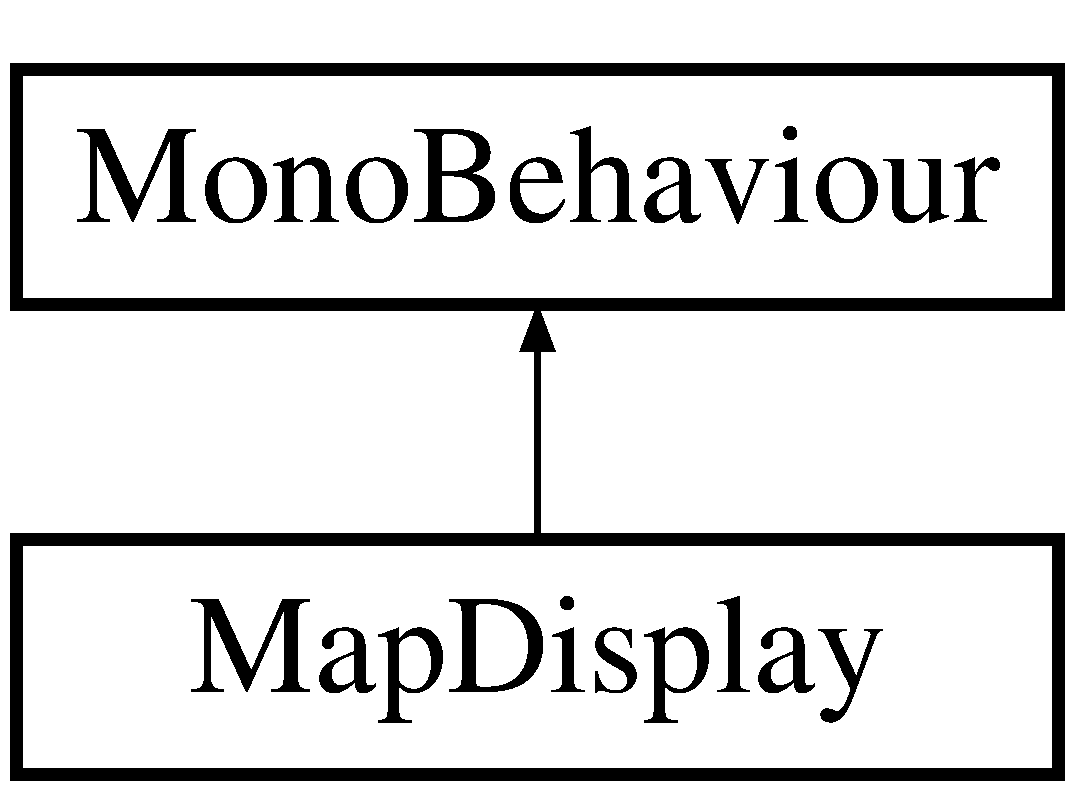
\includegraphics[height=2.000000cm]{class_map_display}
\end{center}
\end{figure}
\subsection*{Public Member Functions}
\begin{DoxyCompactItemize}
\item 
void \mbox{\hyperlink{class_map_display_a27468745a8df537d3da3d0ce5814fc5b}{Draw\+Texture}} (Texture2D texture)
\item 
void \mbox{\hyperlink{class_map_display_a051aac4836942702d88eac0732e0bd52}{Draw\+Mesh}} (\mbox{\hyperlink{class_mesh_data}{Mesh\+Data}} mesh\+Data, Texture2D texture)
\end{DoxyCompactItemize}
\subsection*{Public Attributes}
\begin{DoxyCompactItemize}
\item 
Renderer \mbox{\hyperlink{class_map_display_acb52594fb49690c89c4929a3bbb34b61}{texture\+Render}}
\item 
Mesh\+Filter \mbox{\hyperlink{class_map_display_a56e864aaaecac3844a10fd98a69e0ab0}{mesh\+Filter}}
\item 
Mesh\+Renderer \mbox{\hyperlink{class_map_display_aa517e3c2a6f717cd74a8554e01476a1f}{mesh\+Renderer}}
\end{DoxyCompactItemize}


\subsection{Member Function Documentation}
\mbox{\Hypertarget{class_map_display_a051aac4836942702d88eac0732e0bd52}\label{class_map_display_a051aac4836942702d88eac0732e0bd52}} 
\index{Map\+Display@{Map\+Display}!Draw\+Mesh@{Draw\+Mesh}}
\index{Draw\+Mesh@{Draw\+Mesh}!Map\+Display@{Map\+Display}}
\subsubsection{\texorpdfstring{Draw\+Mesh()}{DrawMesh()}}
{\footnotesize\ttfamily void Map\+Display.\+Draw\+Mesh (\begin{DoxyParamCaption}\item[{\mbox{\hyperlink{class_mesh_data}{Mesh\+Data}}}]{mesh\+Data,  }\item[{Texture2D}]{texture }\end{DoxyParamCaption})}

\mbox{\Hypertarget{class_map_display_a27468745a8df537d3da3d0ce5814fc5b}\label{class_map_display_a27468745a8df537d3da3d0ce5814fc5b}} 
\index{Map\+Display@{Map\+Display}!Draw\+Texture@{Draw\+Texture}}
\index{Draw\+Texture@{Draw\+Texture}!Map\+Display@{Map\+Display}}
\subsubsection{\texorpdfstring{Draw\+Texture()}{DrawTexture()}}
{\footnotesize\ttfamily void Map\+Display.\+Draw\+Texture (\begin{DoxyParamCaption}\item[{Texture2D}]{texture }\end{DoxyParamCaption})}



\subsection{Member Data Documentation}
\mbox{\Hypertarget{class_map_display_a56e864aaaecac3844a10fd98a69e0ab0}\label{class_map_display_a56e864aaaecac3844a10fd98a69e0ab0}} 
\index{Map\+Display@{Map\+Display}!mesh\+Filter@{mesh\+Filter}}
\index{mesh\+Filter@{mesh\+Filter}!Map\+Display@{Map\+Display}}
\subsubsection{\texorpdfstring{mesh\+Filter}{meshFilter}}
{\footnotesize\ttfamily Mesh\+Filter Map\+Display.\+mesh\+Filter}

\mbox{\Hypertarget{class_map_display_aa517e3c2a6f717cd74a8554e01476a1f}\label{class_map_display_aa517e3c2a6f717cd74a8554e01476a1f}} 
\index{Map\+Display@{Map\+Display}!mesh\+Renderer@{mesh\+Renderer}}
\index{mesh\+Renderer@{mesh\+Renderer}!Map\+Display@{Map\+Display}}
\subsubsection{\texorpdfstring{mesh\+Renderer}{meshRenderer}}
{\footnotesize\ttfamily Mesh\+Renderer Map\+Display.\+mesh\+Renderer}

\mbox{\Hypertarget{class_map_display_acb52594fb49690c89c4929a3bbb34b61}\label{class_map_display_acb52594fb49690c89c4929a3bbb34b61}} 
\index{Map\+Display@{Map\+Display}!texture\+Render@{texture\+Render}}
\index{texture\+Render@{texture\+Render}!Map\+Display@{Map\+Display}}
\subsubsection{\texorpdfstring{texture\+Render}{textureRender}}
{\footnotesize\ttfamily Renderer Map\+Display.\+texture\+Render}



The documentation for this class was generated from the following file\+:\begin{DoxyCompactItemize}
\item 
/\+Users/sabienambrose/\+Documents/\+Coding/\+Unity\+Mechanical\+Turk/\+Mechanical\+Turk/\+Assets/\+Scripts/\mbox{\hyperlink{_map_display_8cs}{Map\+Display.\+cs}}\end{DoxyCompactItemize}

\hypertarget{class_map_generator}{}\section{Map\+Generator Class Reference}
\label{class_map_generator}\index{Map\+Generator@{Map\+Generator}}
Inheritance diagram for Map\+Generator\+:\begin{figure}[H]
\begin{center}
\leavevmode
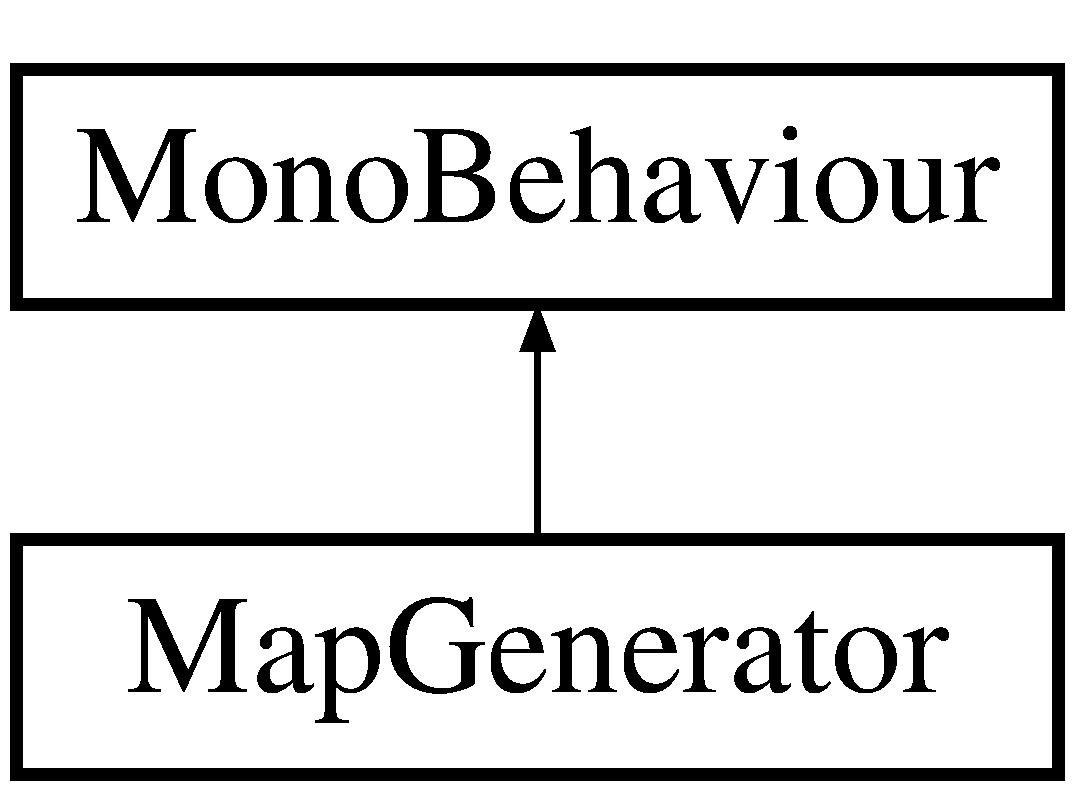
\includegraphics[height=2.000000cm]{class_map_generator}
\end{center}
\end{figure}
\subsection*{Public Types}
\begin{DoxyCompactItemize}
\item 
enum \mbox{\hyperlink{class_map_generator_ad11b508087506616937d0dac5576c2ab}{Draw\+Mode}} \{ \mbox{\hyperlink{class_map_generator_ad11b508087506616937d0dac5576c2abaf1b803399772ec7c6b60c4dd5ee008e3}{Draw\+Mode.\+Noise\+Map}}, 
\mbox{\hyperlink{class_map_generator_ad11b508087506616937d0dac5576c2abaf0a9eaea3a84d380edf51e2f1236abd0}{Draw\+Mode.\+Colour\+Map}}, 
\mbox{\hyperlink{class_map_generator_ad11b508087506616937d0dac5576c2aba710fdb6adb881b408116ef95335e1961}{Draw\+Mode.\+Mesh}}
 \}
\end{DoxyCompactItemize}
\subsection*{Public Member Functions}
\begin{DoxyCompactItemize}
\item 
void \mbox{\hyperlink{class_map_generator_adc8f9ffbc33e6d4b1593900c3059fdf7}{Generate\+Map}} ()
\item 
void \mbox{\hyperlink{class_map_generator_ac6e51a7c21ff6e6bae4ae637536b4c53}{Generate\+Map}} (float\mbox{[},\mbox{]} noise\+Map)
\item 
Color \mbox{[}$\,$\mbox{]} \mbox{\hyperlink{class_map_generator_acfc52dd649037da30a270b6347b6c436}{Get\+Color\+Map}} (\mbox{\hyperlink{class_noise_map}{Noise\+Map}} noise\+Map)
\end{DoxyCompactItemize}
\subsection*{Public Attributes}
\begin{DoxyCompactItemize}
\item 
\mbox{\hyperlink{class_map_generator_ad11b508087506616937d0dac5576c2ab}{Draw\+Mode}} \mbox{\hyperlink{class_map_generator_ab7abc6f55e460a0778c8f9fb0922c0b2}{draw\+Mode}}
\item 
int \mbox{\hyperlink{class_map_generator_a36dc6ed804922345576a48c92ca2a7c5}{level\+Of\+Detail}}
\item 
float \mbox{\hyperlink{class_map_generator_a240eb7cb057720f6b650ba7f89f73857}{noise\+Scale}}
\item 
int \mbox{\hyperlink{class_map_generator_a89c8da977598552d30b0110669b09960}{octaves}}
\item 
float \mbox{\hyperlink{class_map_generator_afc59b0a77b7165a6654e08d0e8580e60}{persistance}}
\item 
float \mbox{\hyperlink{class_map_generator_ada5f0345bb8a65536c3aa911f63565af}{lacunarity}}
\item 
int \mbox{\hyperlink{class_map_generator_a7ad3b7337f5252b30d873f0d76a06fcb}{seed}}
\item 
Vector2 \mbox{\hyperlink{class_map_generator_a785c0d701c764003f0c7dfdd3be5077c}{offset}}
\item 
float \mbox{\hyperlink{class_map_generator_ad0ea5ea76e455736a4b831774fca1029}{mesh\+Height\+Multiplier}}
\item 
Animation\+Curve \mbox{\hyperlink{class_map_generator_a814ef92c835bac7d01e4c839bd4580ab}{mesh\+Height\+Curve}}
\item 
bool \mbox{\hyperlink{class_map_generator_af0843909ea371f9eee073691750482c3}{auto\+Update}}
\item 
\mbox{\hyperlink{struct_terrain_type}{Terrain\+Type}} \mbox{[}$\,$\mbox{]} \mbox{\hyperlink{class_map_generator_adaca0c66c3812a547927a6fcdd353dc7}{regions}}
\end{DoxyCompactItemize}


\subsection{Member Enumeration Documentation}
\mbox{\Hypertarget{class_map_generator_ad11b508087506616937d0dac5576c2ab}\label{class_map_generator_ad11b508087506616937d0dac5576c2ab}} 
\index{Map\+Generator@{Map\+Generator}!Draw\+Mode@{Draw\+Mode}}
\index{Draw\+Mode@{Draw\+Mode}!Map\+Generator@{Map\+Generator}}
\subsubsection{\texorpdfstring{Draw\+Mode}{DrawMode}}
{\footnotesize\ttfamily enum \mbox{\hyperlink{class_map_generator_ad11b508087506616937d0dac5576c2ab}{Map\+Generator.\+Draw\+Mode}}\hspace{0.3cm}{\ttfamily [strong]}}

\begin{DoxyEnumFields}{Enumerator}
\raisebox{\heightof{T}}[0pt][0pt]{\index{Noise\+Map@{Noise\+Map}!Map\+Generator@{Map\+Generator}}\index{Map\+Generator@{Map\+Generator}!Noise\+Map@{Noise\+Map}}}\mbox{\Hypertarget{class_map_generator_ad11b508087506616937d0dac5576c2abaf1b803399772ec7c6b60c4dd5ee008e3}\label{class_map_generator_ad11b508087506616937d0dac5576c2abaf1b803399772ec7c6b60c4dd5ee008e3}} 
Noise\+Map&\\
\hline

\raisebox{\heightof{T}}[0pt][0pt]{\index{Colour\+Map@{Colour\+Map}!Map\+Generator@{Map\+Generator}}\index{Map\+Generator@{Map\+Generator}!Colour\+Map@{Colour\+Map}}}\mbox{\Hypertarget{class_map_generator_ad11b508087506616937d0dac5576c2abaf0a9eaea3a84d380edf51e2f1236abd0}\label{class_map_generator_ad11b508087506616937d0dac5576c2abaf0a9eaea3a84d380edf51e2f1236abd0}} 
Colour\+Map&\\
\hline

\raisebox{\heightof{T}}[0pt][0pt]{\index{Mesh@{Mesh}!Map\+Generator@{Map\+Generator}}\index{Map\+Generator@{Map\+Generator}!Mesh@{Mesh}}}\mbox{\Hypertarget{class_map_generator_ad11b508087506616937d0dac5576c2aba710fdb6adb881b408116ef95335e1961}\label{class_map_generator_ad11b508087506616937d0dac5576c2aba710fdb6adb881b408116ef95335e1961}} 
Mesh&\\
\hline

\end{DoxyEnumFields}


\subsection{Member Function Documentation}
\mbox{\Hypertarget{class_map_generator_adc8f9ffbc33e6d4b1593900c3059fdf7}\label{class_map_generator_adc8f9ffbc33e6d4b1593900c3059fdf7}} 
\index{Map\+Generator@{Map\+Generator}!Generate\+Map@{Generate\+Map}}
\index{Generate\+Map@{Generate\+Map}!Map\+Generator@{Map\+Generator}}
\subsubsection{\texorpdfstring{Generate\+Map()}{GenerateMap()}\hspace{0.1cm}{\footnotesize\ttfamily [1/2]}}
{\footnotesize\ttfamily void Map\+Generator.\+Generate\+Map (\begin{DoxyParamCaption}{ }\end{DoxyParamCaption})}

\mbox{\Hypertarget{class_map_generator_ac6e51a7c21ff6e6bae4ae637536b4c53}\label{class_map_generator_ac6e51a7c21ff6e6bae4ae637536b4c53}} 
\index{Map\+Generator@{Map\+Generator}!Generate\+Map@{Generate\+Map}}
\index{Generate\+Map@{Generate\+Map}!Map\+Generator@{Map\+Generator}}
\subsubsection{\texorpdfstring{Generate\+Map()}{GenerateMap()}\hspace{0.1cm}{\footnotesize\ttfamily [2/2]}}
{\footnotesize\ttfamily void Map\+Generator.\+Generate\+Map (\begin{DoxyParamCaption}\item[{float}]{noise\+Map\mbox{[},\mbox{]} }\end{DoxyParamCaption})}

\mbox{\Hypertarget{class_map_generator_acfc52dd649037da30a270b6347b6c436}\label{class_map_generator_acfc52dd649037da30a270b6347b6c436}} 
\index{Map\+Generator@{Map\+Generator}!Get\+Color\+Map@{Get\+Color\+Map}}
\index{Get\+Color\+Map@{Get\+Color\+Map}!Map\+Generator@{Map\+Generator}}
\subsubsection{\texorpdfstring{Get\+Color\+Map()}{GetColorMap()}}
{\footnotesize\ttfamily Color \mbox{[}$\,$\mbox{]} Map\+Generator.\+Get\+Color\+Map (\begin{DoxyParamCaption}\item[{\mbox{\hyperlink{class_noise_map}{Noise\+Map}}}]{noise\+Map }\end{DoxyParamCaption})}



\subsection{Member Data Documentation}
\mbox{\Hypertarget{class_map_generator_af0843909ea371f9eee073691750482c3}\label{class_map_generator_af0843909ea371f9eee073691750482c3}} 
\index{Map\+Generator@{Map\+Generator}!auto\+Update@{auto\+Update}}
\index{auto\+Update@{auto\+Update}!Map\+Generator@{Map\+Generator}}
\subsubsection{\texorpdfstring{auto\+Update}{autoUpdate}}
{\footnotesize\ttfamily bool Map\+Generator.\+auto\+Update}

\mbox{\Hypertarget{class_map_generator_ab7abc6f55e460a0778c8f9fb0922c0b2}\label{class_map_generator_ab7abc6f55e460a0778c8f9fb0922c0b2}} 
\index{Map\+Generator@{Map\+Generator}!draw\+Mode@{draw\+Mode}}
\index{draw\+Mode@{draw\+Mode}!Map\+Generator@{Map\+Generator}}
\subsubsection{\texorpdfstring{draw\+Mode}{drawMode}}
{\footnotesize\ttfamily \mbox{\hyperlink{class_map_generator_ad11b508087506616937d0dac5576c2ab}{Draw\+Mode}} Map\+Generator.\+draw\+Mode}

\mbox{\Hypertarget{class_map_generator_ada5f0345bb8a65536c3aa911f63565af}\label{class_map_generator_ada5f0345bb8a65536c3aa911f63565af}} 
\index{Map\+Generator@{Map\+Generator}!lacunarity@{lacunarity}}
\index{lacunarity@{lacunarity}!Map\+Generator@{Map\+Generator}}
\subsubsection{\texorpdfstring{lacunarity}{lacunarity}}
{\footnotesize\ttfamily float Map\+Generator.\+lacunarity}

\mbox{\Hypertarget{class_map_generator_a36dc6ed804922345576a48c92ca2a7c5}\label{class_map_generator_a36dc6ed804922345576a48c92ca2a7c5}} 
\index{Map\+Generator@{Map\+Generator}!level\+Of\+Detail@{level\+Of\+Detail}}
\index{level\+Of\+Detail@{level\+Of\+Detail}!Map\+Generator@{Map\+Generator}}
\subsubsection{\texorpdfstring{level\+Of\+Detail}{levelOfDetail}}
{\footnotesize\ttfamily int Map\+Generator.\+level\+Of\+Detail}

\mbox{\Hypertarget{class_map_generator_a814ef92c835bac7d01e4c839bd4580ab}\label{class_map_generator_a814ef92c835bac7d01e4c839bd4580ab}} 
\index{Map\+Generator@{Map\+Generator}!mesh\+Height\+Curve@{mesh\+Height\+Curve}}
\index{mesh\+Height\+Curve@{mesh\+Height\+Curve}!Map\+Generator@{Map\+Generator}}
\subsubsection{\texorpdfstring{mesh\+Height\+Curve}{meshHeightCurve}}
{\footnotesize\ttfamily Animation\+Curve Map\+Generator.\+mesh\+Height\+Curve}

\mbox{\Hypertarget{class_map_generator_ad0ea5ea76e455736a4b831774fca1029}\label{class_map_generator_ad0ea5ea76e455736a4b831774fca1029}} 
\index{Map\+Generator@{Map\+Generator}!mesh\+Height\+Multiplier@{mesh\+Height\+Multiplier}}
\index{mesh\+Height\+Multiplier@{mesh\+Height\+Multiplier}!Map\+Generator@{Map\+Generator}}
\subsubsection{\texorpdfstring{mesh\+Height\+Multiplier}{meshHeightMultiplier}}
{\footnotesize\ttfamily float Map\+Generator.\+mesh\+Height\+Multiplier}

\mbox{\Hypertarget{class_map_generator_a240eb7cb057720f6b650ba7f89f73857}\label{class_map_generator_a240eb7cb057720f6b650ba7f89f73857}} 
\index{Map\+Generator@{Map\+Generator}!noise\+Scale@{noise\+Scale}}
\index{noise\+Scale@{noise\+Scale}!Map\+Generator@{Map\+Generator}}
\subsubsection{\texorpdfstring{noise\+Scale}{noiseScale}}
{\footnotesize\ttfamily float Map\+Generator.\+noise\+Scale}

\mbox{\Hypertarget{class_map_generator_a89c8da977598552d30b0110669b09960}\label{class_map_generator_a89c8da977598552d30b0110669b09960}} 
\index{Map\+Generator@{Map\+Generator}!octaves@{octaves}}
\index{octaves@{octaves}!Map\+Generator@{Map\+Generator}}
\subsubsection{\texorpdfstring{octaves}{octaves}}
{\footnotesize\ttfamily int Map\+Generator.\+octaves}

\mbox{\Hypertarget{class_map_generator_a785c0d701c764003f0c7dfdd3be5077c}\label{class_map_generator_a785c0d701c764003f0c7dfdd3be5077c}} 
\index{Map\+Generator@{Map\+Generator}!offset@{offset}}
\index{offset@{offset}!Map\+Generator@{Map\+Generator}}
\subsubsection{\texorpdfstring{offset}{offset}}
{\footnotesize\ttfamily Vector2 Map\+Generator.\+offset}

\mbox{\Hypertarget{class_map_generator_afc59b0a77b7165a6654e08d0e8580e60}\label{class_map_generator_afc59b0a77b7165a6654e08d0e8580e60}} 
\index{Map\+Generator@{Map\+Generator}!persistance@{persistance}}
\index{persistance@{persistance}!Map\+Generator@{Map\+Generator}}
\subsubsection{\texorpdfstring{persistance}{persistance}}
{\footnotesize\ttfamily float Map\+Generator.\+persistance}

\mbox{\Hypertarget{class_map_generator_adaca0c66c3812a547927a6fcdd353dc7}\label{class_map_generator_adaca0c66c3812a547927a6fcdd353dc7}} 
\index{Map\+Generator@{Map\+Generator}!regions@{regions}}
\index{regions@{regions}!Map\+Generator@{Map\+Generator}}
\subsubsection{\texorpdfstring{regions}{regions}}
{\footnotesize\ttfamily \mbox{\hyperlink{struct_terrain_type}{Terrain\+Type}} \mbox{[}$\,$\mbox{]} Map\+Generator.\+regions}

\mbox{\Hypertarget{class_map_generator_a7ad3b7337f5252b30d873f0d76a06fcb}\label{class_map_generator_a7ad3b7337f5252b30d873f0d76a06fcb}} 
\index{Map\+Generator@{Map\+Generator}!seed@{seed}}
\index{seed@{seed}!Map\+Generator@{Map\+Generator}}
\subsubsection{\texorpdfstring{seed}{seed}}
{\footnotesize\ttfamily int Map\+Generator.\+seed}



The documentation for this class was generated from the following file\+:\begin{DoxyCompactItemize}
\item 
/\+Users/sabienambrose/\+Documents/\+Coding/\+Unity\+Mechanical\+Turk/\+Mechanical\+Turk/\+Assets/\+Scripts/\+Generation/\mbox{\hyperlink{_map_generator_8cs}{Map\+Generator.\+cs}}\end{DoxyCompactItemize}

\hypertarget{class_math_ops}{}\section{Math\+Ops Class Reference}
\label{class_math_ops}\index{Math\+Ops@{Math\+Ops}}
\subsection*{Static Public Member Functions}
\begin{DoxyCompactItemize}
\item 
static Vector2 \mbox{\hyperlink{class_math_ops_a375da2b95a7a9cc75dd9413e2f6521d1}{Midpoint}} (Vector2 A, Vector2 B)
\item 
static float \mbox{\hyperlink{class_math_ops_a8143187da9ccc8eb4d7e2e6d89f2008b}{Bisector\+Slope}} (Vector2 A, Vector2 B)
\item 
static float \mbox{\hyperlink{class_math_ops_af1a2e97f206740e26a569a07a663de7d}{Slope}} (Vector2 A, Vector2 B)
\item 
static float \mbox{\hyperlink{class_math_ops_a5eb232eb24001f54d3ff3d3dc19adf3c}{Bisector\+Const}} (Vector2 \mbox{\hyperlink{class_math_ops_a375da2b95a7a9cc75dd9413e2f6521d1}{Midpoint}}, float slope)
\item 
static Vector2 \mbox{\hyperlink{class_math_ops_aac4861e44cbbf5c8e3f8e7aee06d5ed0}{Circum\+Center}} (Vector2 A, Vector2 B, Vector2 C)
\item 
static float \mbox{\hyperlink{class_math_ops_a79f3f44aa12a5804b6e6ff7874c62cbd}{Circum\+Radius}} (Vector2 A, Vector2 B, Vector2 C)
\item 
static bool \mbox{\hyperlink{class_math_ops_a8add15f1367d790bc4ba29331a72bd32}{Is\+Point\+In\+Circumcircle}} (Vector2 P, Vector2 A, Vector2 B, Vector2 C)
\item 
static Vector3 \mbox{\hyperlink{class_math_ops_ab1c0982b962841b8e0e0505a30032091}{Flip\+YZ}} (Vector3 P)
\end{DoxyCompactItemize}


\subsection{Member Function Documentation}
\mbox{\Hypertarget{class_math_ops_a5eb232eb24001f54d3ff3d3dc19adf3c}\label{class_math_ops_a5eb232eb24001f54d3ff3d3dc19adf3c}} 
\index{Math\+Ops@{Math\+Ops}!Bisector\+Const@{Bisector\+Const}}
\index{Bisector\+Const@{Bisector\+Const}!Math\+Ops@{Math\+Ops}}
\subsubsection{\texorpdfstring{Bisector\+Const()}{BisectorConst()}}
{\footnotesize\ttfamily static float Math\+Ops.\+Bisector\+Const (\begin{DoxyParamCaption}\item[{Vector2}]{Midpoint,  }\item[{float}]{slope }\end{DoxyParamCaption})\hspace{0.3cm}{\ttfamily [static]}}

\mbox{\Hypertarget{class_math_ops_a8143187da9ccc8eb4d7e2e6d89f2008b}\label{class_math_ops_a8143187da9ccc8eb4d7e2e6d89f2008b}} 
\index{Math\+Ops@{Math\+Ops}!Bisector\+Slope@{Bisector\+Slope}}
\index{Bisector\+Slope@{Bisector\+Slope}!Math\+Ops@{Math\+Ops}}
\subsubsection{\texorpdfstring{Bisector\+Slope()}{BisectorSlope()}}
{\footnotesize\ttfamily static float Math\+Ops.\+Bisector\+Slope (\begin{DoxyParamCaption}\item[{Vector2}]{A,  }\item[{Vector2}]{B }\end{DoxyParamCaption})\hspace{0.3cm}{\ttfamily [static]}}

\mbox{\Hypertarget{class_math_ops_aac4861e44cbbf5c8e3f8e7aee06d5ed0}\label{class_math_ops_aac4861e44cbbf5c8e3f8e7aee06d5ed0}} 
\index{Math\+Ops@{Math\+Ops}!Circum\+Center@{Circum\+Center}}
\index{Circum\+Center@{Circum\+Center}!Math\+Ops@{Math\+Ops}}
\subsubsection{\texorpdfstring{Circum\+Center()}{CircumCenter()}}
{\footnotesize\ttfamily static Vector2 Math\+Ops.\+Circum\+Center (\begin{DoxyParamCaption}\item[{Vector2}]{A,  }\item[{Vector2}]{B,  }\item[{Vector2}]{C }\end{DoxyParamCaption})\hspace{0.3cm}{\ttfamily [static]}}

\mbox{\Hypertarget{class_math_ops_a79f3f44aa12a5804b6e6ff7874c62cbd}\label{class_math_ops_a79f3f44aa12a5804b6e6ff7874c62cbd}} 
\index{Math\+Ops@{Math\+Ops}!Circum\+Radius@{Circum\+Radius}}
\index{Circum\+Radius@{Circum\+Radius}!Math\+Ops@{Math\+Ops}}
\subsubsection{\texorpdfstring{Circum\+Radius()}{CircumRadius()}}
{\footnotesize\ttfamily static float Math\+Ops.\+Circum\+Radius (\begin{DoxyParamCaption}\item[{Vector2}]{A,  }\item[{Vector2}]{B,  }\item[{Vector2}]{C }\end{DoxyParamCaption})\hspace{0.3cm}{\ttfamily [static]}}

\mbox{\Hypertarget{class_math_ops_ab1c0982b962841b8e0e0505a30032091}\label{class_math_ops_ab1c0982b962841b8e0e0505a30032091}} 
\index{Math\+Ops@{Math\+Ops}!Flip\+YZ@{Flip\+YZ}}
\index{Flip\+YZ@{Flip\+YZ}!Math\+Ops@{Math\+Ops}}
\subsubsection{\texorpdfstring{Flip\+Y\+Z()}{FlipYZ()}}
{\footnotesize\ttfamily static Vector3 Math\+Ops.\+Flip\+YZ (\begin{DoxyParamCaption}\item[{Vector3}]{P }\end{DoxyParamCaption})\hspace{0.3cm}{\ttfamily [static]}}

\mbox{\Hypertarget{class_math_ops_a8add15f1367d790bc4ba29331a72bd32}\label{class_math_ops_a8add15f1367d790bc4ba29331a72bd32}} 
\index{Math\+Ops@{Math\+Ops}!Is\+Point\+In\+Circumcircle@{Is\+Point\+In\+Circumcircle}}
\index{Is\+Point\+In\+Circumcircle@{Is\+Point\+In\+Circumcircle}!Math\+Ops@{Math\+Ops}}
\subsubsection{\texorpdfstring{Is\+Point\+In\+Circumcircle()}{IsPointInCircumcircle()}}
{\footnotesize\ttfamily static bool Math\+Ops.\+Is\+Point\+In\+Circumcircle (\begin{DoxyParamCaption}\item[{Vector2}]{P,  }\item[{Vector2}]{A,  }\item[{Vector2}]{B,  }\item[{Vector2}]{C }\end{DoxyParamCaption})\hspace{0.3cm}{\ttfamily [static]}}

\mbox{\Hypertarget{class_math_ops_a375da2b95a7a9cc75dd9413e2f6521d1}\label{class_math_ops_a375da2b95a7a9cc75dd9413e2f6521d1}} 
\index{Math\+Ops@{Math\+Ops}!Midpoint@{Midpoint}}
\index{Midpoint@{Midpoint}!Math\+Ops@{Math\+Ops}}
\subsubsection{\texorpdfstring{Midpoint()}{Midpoint()}}
{\footnotesize\ttfamily static Vector2 Math\+Ops.\+Midpoint (\begin{DoxyParamCaption}\item[{Vector2}]{A,  }\item[{Vector2}]{B }\end{DoxyParamCaption})\hspace{0.3cm}{\ttfamily [static]}}

\mbox{\Hypertarget{class_math_ops_af1a2e97f206740e26a569a07a663de7d}\label{class_math_ops_af1a2e97f206740e26a569a07a663de7d}} 
\index{Math\+Ops@{Math\+Ops}!Slope@{Slope}}
\index{Slope@{Slope}!Math\+Ops@{Math\+Ops}}
\subsubsection{\texorpdfstring{Slope()}{Slope()}}
{\footnotesize\ttfamily static float Math\+Ops.\+Slope (\begin{DoxyParamCaption}\item[{Vector2}]{A,  }\item[{Vector2}]{B }\end{DoxyParamCaption})\hspace{0.3cm}{\ttfamily [static]}}



The documentation for this class was generated from the following file\+:\begin{DoxyCompactItemize}
\item 
/\+Users/sabienambrose/\+Documents/\+Coding/\+Unity\+Mechanical\+Turk/\+Mechanical\+Turk/\+Assets/\+Scripts/\+Util/\mbox{\hyperlink{_math_ops_8cs}{Math\+Ops.\+cs}}\end{DoxyCompactItemize}

\hypertarget{class_mesh_data}{}\section{Mesh\+Data Class Reference}
\label{class_mesh_data}\index{Mesh\+Data@{Mesh\+Data}}
\subsection*{Public Member Functions}
\begin{DoxyCompactItemize}
\item 
\mbox{\hyperlink{class_mesh_data_a6a44cce7c0e7f8f229ee3be7d0590628}{Mesh\+Data}} (int mesh\+Width, int mesh\+Height)
\item 
void \mbox{\hyperlink{class_mesh_data_a1515ec040fe2639c6635564eea60979f}{Add\+Triangle}} (int a, int b, int c)
\item 
Mesh \mbox{\hyperlink{class_mesh_data_a9d813c3b2d1b1eb78bfcaaf11e04cf63}{Create\+Mesh}} ()
\end{DoxyCompactItemize}
\subsection*{Public Attributes}
\begin{DoxyCompactItemize}
\item 
Vector3 \mbox{[}$\,$\mbox{]} \mbox{\hyperlink{class_mesh_data_ae3f35f48b31703208a848cf265daa11b}{vertices}}
\item 
int \mbox{[}$\,$\mbox{]} \mbox{\hyperlink{class_mesh_data_af129fc7adecb83908ea1a4c1c3a1fdc0}{triangles}}
\item 
Vector2 \mbox{[}$\,$\mbox{]} \mbox{\hyperlink{class_mesh_data_aa3e087dedb7d67e1bd3cfb98ec50f13c}{uvs}}
\end{DoxyCompactItemize}


\subsection{Constructor \& Destructor Documentation}
\mbox{\Hypertarget{class_mesh_data_a6a44cce7c0e7f8f229ee3be7d0590628}\label{class_mesh_data_a6a44cce7c0e7f8f229ee3be7d0590628}} 
\index{Mesh\+Data@{Mesh\+Data}!Mesh\+Data@{Mesh\+Data}}
\index{Mesh\+Data@{Mesh\+Data}!Mesh\+Data@{Mesh\+Data}}
\subsubsection{\texorpdfstring{Mesh\+Data()}{MeshData()}}
{\footnotesize\ttfamily Mesh\+Data.\+Mesh\+Data (\begin{DoxyParamCaption}\item[{int}]{mesh\+Width,  }\item[{int}]{mesh\+Height }\end{DoxyParamCaption})}



\subsection{Member Function Documentation}
\mbox{\Hypertarget{class_mesh_data_a1515ec040fe2639c6635564eea60979f}\label{class_mesh_data_a1515ec040fe2639c6635564eea60979f}} 
\index{Mesh\+Data@{Mesh\+Data}!Add\+Triangle@{Add\+Triangle}}
\index{Add\+Triangle@{Add\+Triangle}!Mesh\+Data@{Mesh\+Data}}
\subsubsection{\texorpdfstring{Add\+Triangle()}{AddTriangle()}}
{\footnotesize\ttfamily void Mesh\+Data.\+Add\+Triangle (\begin{DoxyParamCaption}\item[{int}]{a,  }\item[{int}]{b,  }\item[{int}]{c }\end{DoxyParamCaption})}

\mbox{\Hypertarget{class_mesh_data_a9d813c3b2d1b1eb78bfcaaf11e04cf63}\label{class_mesh_data_a9d813c3b2d1b1eb78bfcaaf11e04cf63}} 
\index{Mesh\+Data@{Mesh\+Data}!Create\+Mesh@{Create\+Mesh}}
\index{Create\+Mesh@{Create\+Mesh}!Mesh\+Data@{Mesh\+Data}}
\subsubsection{\texorpdfstring{Create\+Mesh()}{CreateMesh()}}
{\footnotesize\ttfamily Mesh Mesh\+Data.\+Create\+Mesh (\begin{DoxyParamCaption}{ }\end{DoxyParamCaption})}



\subsection{Member Data Documentation}
\mbox{\Hypertarget{class_mesh_data_af129fc7adecb83908ea1a4c1c3a1fdc0}\label{class_mesh_data_af129fc7adecb83908ea1a4c1c3a1fdc0}} 
\index{Mesh\+Data@{Mesh\+Data}!triangles@{triangles}}
\index{triangles@{triangles}!Mesh\+Data@{Mesh\+Data}}
\subsubsection{\texorpdfstring{triangles}{triangles}}
{\footnotesize\ttfamily int \mbox{[}$\,$\mbox{]} Mesh\+Data.\+triangles}

\mbox{\Hypertarget{class_mesh_data_aa3e087dedb7d67e1bd3cfb98ec50f13c}\label{class_mesh_data_aa3e087dedb7d67e1bd3cfb98ec50f13c}} 
\index{Mesh\+Data@{Mesh\+Data}!uvs@{uvs}}
\index{uvs@{uvs}!Mesh\+Data@{Mesh\+Data}}
\subsubsection{\texorpdfstring{uvs}{uvs}}
{\footnotesize\ttfamily Vector2 \mbox{[}$\,$\mbox{]} Mesh\+Data.\+uvs}

\mbox{\Hypertarget{class_mesh_data_ae3f35f48b31703208a848cf265daa11b}\label{class_mesh_data_ae3f35f48b31703208a848cf265daa11b}} 
\index{Mesh\+Data@{Mesh\+Data}!vertices@{vertices}}
\index{vertices@{vertices}!Mesh\+Data@{Mesh\+Data}}
\subsubsection{\texorpdfstring{vertices}{vertices}}
{\footnotesize\ttfamily Vector3 \mbox{[}$\,$\mbox{]} Mesh\+Data.\+vertices}



The documentation for this class was generated from the following file\+:\begin{DoxyCompactItemize}
\item 
/\+Users/sabienambrose/\+Documents/\+Coding/\+Unity\+Mechanical\+Turk/\+Mechanical\+Turk/\+Assets/\+Scripts/\+Generation/\mbox{\hyperlink{_mesh_generator_8cs}{Mesh\+Generator.\+cs}}\end{DoxyCompactItemize}

\hypertarget{class_node}{}\section{Node Class Reference}
\label{class_node}\index{Node@{Node}}
Inheritance diagram for Node\+:\begin{figure}[H]
\begin{center}
\leavevmode
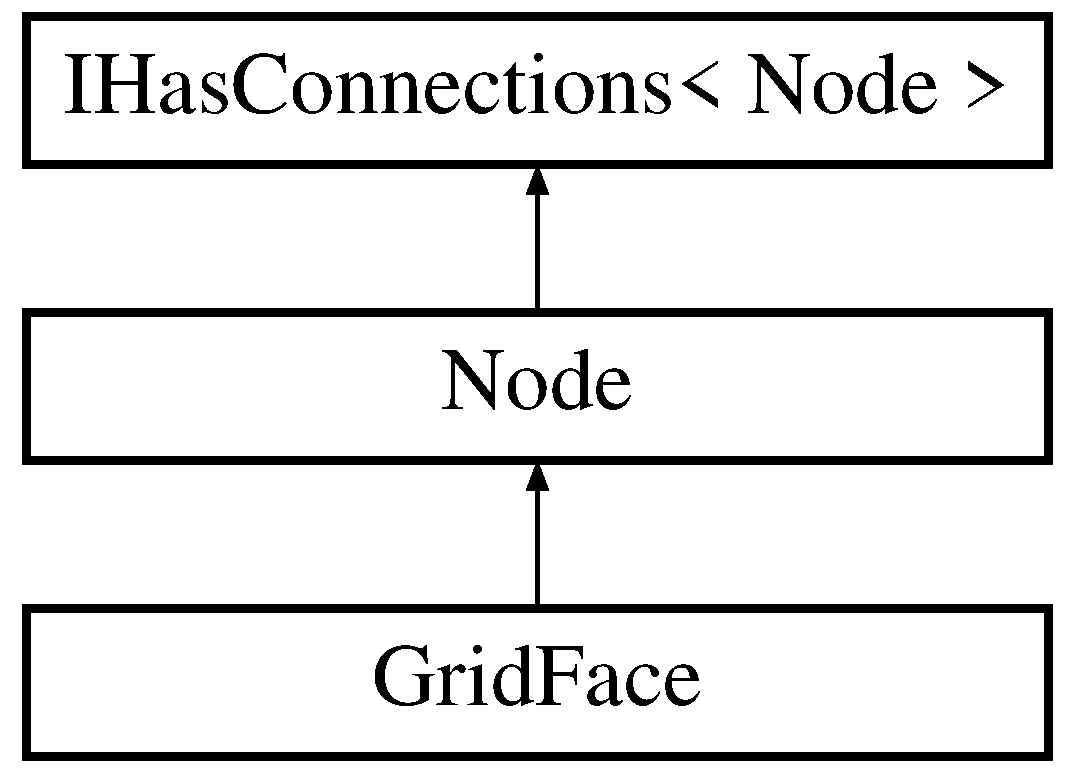
\includegraphics[height=3.000000cm]{class_node}
\end{center}
\end{figure}
\subsection*{Public Member Functions}
\begin{DoxyCompactItemize}
\item 
\mbox{\hyperlink{class_node_a989164b636cfeff98b4df9833976f4f5}{Node}} ()
\item 
\mbox{\hyperlink{class_node_a653c96cdaab99419a8c1d8d80be10b80}{Node}} (Vector2 position2)
\item 
\mbox{\hyperlink{class_node_a188e8794e019e1dd2fcfa84af795c06d}{Node}} (Vector3 \mbox{\hyperlink{class_node_a315059cd3874b8ca61426a4e1bd097a7}{position}})
\item 
void \mbox{\hyperlink{class_node_adaf109cc39cf2444181ea55985767cee}{Add\+Connection}} (\mbox{\hyperlink{class_node}{Node}} connection)
\begin{DoxyCompactList}\small\item\em Adds \mbox{\hyperlink{class_node_edge}{Node\+Edge}} to edges as well as to \textquotesingle{}s edges. \end{DoxyCompactList}\item 
void \mbox{\hyperlink{class_node_ac11a8a128533ef77b42e97d883ab0825}{Remove\+Connection}} (\mbox{\hyperlink{class_node}{Node}} connection)
\item 
bool \mbox{\hyperlink{class_node_a60543d6f014ce3e5d201108949bec386}{Is\+Null\+Or\+This}} (\mbox{\hyperlink{class_node}{Node}} c)
\item 
int \mbox{\hyperlink{class_node_adfa9ae31ba9f758335618f4928d9d4a0}{Index\+Of}} (\mbox{\hyperlink{class_node}{Node}} other)
\item 
bool \mbox{\hyperlink{class_node_acf505ea93da66cff664d7195d64c4a5b}{Is\+Connected\+To}} (\mbox{\hyperlink{class_node}{Node}} other)
\item 
int \mbox{\hyperlink{class_node_a229ce68ffe988dbfd45c05b7e7cbdf2d}{Num\+Connections}} ()
\item 
void \mbox{\hyperlink{class_node_a0a14a3bf53ab9b4939fa6518d1fa4278}{Get\+Connections}} (out List$<$ \mbox{\hyperlink{interface_i_connection}{I\+Connection}}$<$ \mbox{\hyperlink{class_node}{Node}} $>$$>$ \mbox{\hyperlink{class_node_a1d236f5a6dd9111a6ed9f2ebbdea57ac}{connections}})
\item 
void \mbox{\hyperlink{class_node_a42ff8a164e2432ceda0f17ab88fa47e1}{Set\+Position}} (Vector3 \mbox{\hyperlink{class_node_a315059cd3874b8ca61426a4e1bd097a7}{position}})
\item 
Vector2 \mbox{\hyperlink{class_node_a1173e5e173312924b2d0d399bf18e246}{Get\+Position\+XZ}} ()
\item 
Vector3 \mbox{\hyperlink{class_node_aba752b203dcf1360d6a9ef80deabd98e}{Get\+Position}} ()
\item 
void \mbox{\hyperlink{class_node_ada2f9aee327ffd50e46684303411b2a8}{Draw\+Connections}} ()
\end{DoxyCompactItemize}
\subsection*{Protected Attributes}
\begin{DoxyCompactItemize}
\item 
Vector3 \mbox{\hyperlink{class_node_a315059cd3874b8ca61426a4e1bd097a7}{position}}
\item 
List$<$ \mbox{\hyperlink{class_node}{Node}} $>$ \mbox{\hyperlink{class_node_a1d236f5a6dd9111a6ed9f2ebbdea57ac}{connections}} =new List$<$\mbox{\hyperlink{class_node}{Node}}$>$()
\end{DoxyCompactItemize}


\subsection{Constructor \& Destructor Documentation}
\mbox{\Hypertarget{class_node_a989164b636cfeff98b4df9833976f4f5}\label{class_node_a989164b636cfeff98b4df9833976f4f5}} 
\index{Node@{Node}!Node@{Node}}
\index{Node@{Node}!Node@{Node}}
\subsubsection{\texorpdfstring{Node()}{Node()}\hspace{0.1cm}{\footnotesize\ttfamily [1/3]}}
{\footnotesize\ttfamily Node.\+Node (\begin{DoxyParamCaption}{ }\end{DoxyParamCaption})}

\mbox{\Hypertarget{class_node_a653c96cdaab99419a8c1d8d80be10b80}\label{class_node_a653c96cdaab99419a8c1d8d80be10b80}} 
\index{Node@{Node}!Node@{Node}}
\index{Node@{Node}!Node@{Node}}
\subsubsection{\texorpdfstring{Node()}{Node()}\hspace{0.1cm}{\footnotesize\ttfamily [2/3]}}
{\footnotesize\ttfamily Node.\+Node (\begin{DoxyParamCaption}\item[{Vector2}]{position2 }\end{DoxyParamCaption})}

\mbox{\Hypertarget{class_node_a188e8794e019e1dd2fcfa84af795c06d}\label{class_node_a188e8794e019e1dd2fcfa84af795c06d}} 
\index{Node@{Node}!Node@{Node}}
\index{Node@{Node}!Node@{Node}}
\subsubsection{\texorpdfstring{Node()}{Node()}\hspace{0.1cm}{\footnotesize\ttfamily [3/3]}}
{\footnotesize\ttfamily Node.\+Node (\begin{DoxyParamCaption}\item[{Vector3}]{position }\end{DoxyParamCaption})}



\subsection{Member Function Documentation}
\mbox{\Hypertarget{class_node_adaf109cc39cf2444181ea55985767cee}\label{class_node_adaf109cc39cf2444181ea55985767cee}} 
\index{Node@{Node}!Add\+Connection@{Add\+Connection}}
\index{Add\+Connection@{Add\+Connection}!Node@{Node}}
\subsubsection{\texorpdfstring{Add\+Connection()}{AddConnection()}}
{\footnotesize\ttfamily void Node.\+Add\+Connection (\begin{DoxyParamCaption}\item[{\mbox{\hyperlink{class_node}{Node}}}]{connection }\end{DoxyParamCaption})}



Adds \mbox{\hyperlink{class_node_edge}{Node\+Edge}} to edges as well as to \textquotesingle{}s edges. 


\begin{DoxyParams}{Parameters}
{\em connection} & The \textquotesingle{}to\textquotesingle{} \mbox{\hyperlink{class_node}{Node}} to add a connection to. \\
\hline
\end{DoxyParams}
\mbox{\Hypertarget{class_node_ada2f9aee327ffd50e46684303411b2a8}\label{class_node_ada2f9aee327ffd50e46684303411b2a8}} 
\index{Node@{Node}!Draw\+Connections@{Draw\+Connections}}
\index{Draw\+Connections@{Draw\+Connections}!Node@{Node}}
\subsubsection{\texorpdfstring{Draw\+Connections()}{DrawConnections()}}
{\footnotesize\ttfamily void Node.\+Draw\+Connections (\begin{DoxyParamCaption}{ }\end{DoxyParamCaption})}

\mbox{\Hypertarget{class_node_a0a14a3bf53ab9b4939fa6518d1fa4278}\label{class_node_a0a14a3bf53ab9b4939fa6518d1fa4278}} 
\index{Node@{Node}!Get\+Connections@{Get\+Connections}}
\index{Get\+Connections@{Get\+Connections}!Node@{Node}}
\subsubsection{\texorpdfstring{Get\+Connections()}{GetConnections()}}
{\footnotesize\ttfamily void Node.\+Get\+Connections (\begin{DoxyParamCaption}\item[{out List$<$ \mbox{\hyperlink{interface_i_connection}{I\+Connection}}$<$ \mbox{\hyperlink{class_node}{Node}} $>$$>$}]{connections }\end{DoxyParamCaption})}

\mbox{\Hypertarget{class_node_aba752b203dcf1360d6a9ef80deabd98e}\label{class_node_aba752b203dcf1360d6a9ef80deabd98e}} 
\index{Node@{Node}!Get\+Position@{Get\+Position}}
\index{Get\+Position@{Get\+Position}!Node@{Node}}
\subsubsection{\texorpdfstring{Get\+Position()}{GetPosition()}}
{\footnotesize\ttfamily Vector3 Node.\+Get\+Position (\begin{DoxyParamCaption}{ }\end{DoxyParamCaption})}

\mbox{\Hypertarget{class_node_a1173e5e173312924b2d0d399bf18e246}\label{class_node_a1173e5e173312924b2d0d399bf18e246}} 
\index{Node@{Node}!Get\+Position\+XZ@{Get\+Position\+XZ}}
\index{Get\+Position\+XZ@{Get\+Position\+XZ}!Node@{Node}}
\subsubsection{\texorpdfstring{Get\+Position\+X\+Z()}{GetPositionXZ()}}
{\footnotesize\ttfamily Vector2 Node.\+Get\+Position\+XZ (\begin{DoxyParamCaption}{ }\end{DoxyParamCaption})}

\mbox{\Hypertarget{class_node_adfa9ae31ba9f758335618f4928d9d4a0}\label{class_node_adfa9ae31ba9f758335618f4928d9d4a0}} 
\index{Node@{Node}!Index\+Of@{Index\+Of}}
\index{Index\+Of@{Index\+Of}!Node@{Node}}
\subsubsection{\texorpdfstring{Index\+Of()}{IndexOf()}}
{\footnotesize\ttfamily int Node.\+Index\+Of (\begin{DoxyParamCaption}\item[{\mbox{\hyperlink{class_node}{Node}}}]{other }\end{DoxyParamCaption})}

\mbox{\Hypertarget{class_node_acf505ea93da66cff664d7195d64c4a5b}\label{class_node_acf505ea93da66cff664d7195d64c4a5b}} 
\index{Node@{Node}!Is\+Connected\+To@{Is\+Connected\+To}}
\index{Is\+Connected\+To@{Is\+Connected\+To}!Node@{Node}}
\subsubsection{\texorpdfstring{Is\+Connected\+To()}{IsConnectedTo()}}
{\footnotesize\ttfamily bool Node.\+Is\+Connected\+To (\begin{DoxyParamCaption}\item[{\mbox{\hyperlink{class_node}{Node}}}]{other }\end{DoxyParamCaption})}

\mbox{\Hypertarget{class_node_a60543d6f014ce3e5d201108949bec386}\label{class_node_a60543d6f014ce3e5d201108949bec386}} 
\index{Node@{Node}!Is\+Null\+Or\+This@{Is\+Null\+Or\+This}}
\index{Is\+Null\+Or\+This@{Is\+Null\+Or\+This}!Node@{Node}}
\subsubsection{\texorpdfstring{Is\+Null\+Or\+This()}{IsNullOrThis()}}
{\footnotesize\ttfamily bool Node.\+Is\+Null\+Or\+This (\begin{DoxyParamCaption}\item[{\mbox{\hyperlink{class_node}{Node}}}]{c }\end{DoxyParamCaption})}

\mbox{\Hypertarget{class_node_a229ce68ffe988dbfd45c05b7e7cbdf2d}\label{class_node_a229ce68ffe988dbfd45c05b7e7cbdf2d}} 
\index{Node@{Node}!Num\+Connections@{Num\+Connections}}
\index{Num\+Connections@{Num\+Connections}!Node@{Node}}
\subsubsection{\texorpdfstring{Num\+Connections()}{NumConnections()}}
{\footnotesize\ttfamily int Node.\+Num\+Connections (\begin{DoxyParamCaption}{ }\end{DoxyParamCaption})}

\mbox{\Hypertarget{class_node_ac11a8a128533ef77b42e97d883ab0825}\label{class_node_ac11a8a128533ef77b42e97d883ab0825}} 
\index{Node@{Node}!Remove\+Connection@{Remove\+Connection}}
\index{Remove\+Connection@{Remove\+Connection}!Node@{Node}}
\subsubsection{\texorpdfstring{Remove\+Connection()}{RemoveConnection()}}
{\footnotesize\ttfamily void Node.\+Remove\+Connection (\begin{DoxyParamCaption}\item[{\mbox{\hyperlink{class_node}{Node}}}]{connection }\end{DoxyParamCaption})}

\mbox{\Hypertarget{class_node_a42ff8a164e2432ceda0f17ab88fa47e1}\label{class_node_a42ff8a164e2432ceda0f17ab88fa47e1}} 
\index{Node@{Node}!Set\+Position@{Set\+Position}}
\index{Set\+Position@{Set\+Position}!Node@{Node}}
\subsubsection{\texorpdfstring{Set\+Position()}{SetPosition()}}
{\footnotesize\ttfamily void Node.\+Set\+Position (\begin{DoxyParamCaption}\item[{Vector3}]{position }\end{DoxyParamCaption})}



\subsection{Member Data Documentation}
\mbox{\Hypertarget{class_node_a1d236f5a6dd9111a6ed9f2ebbdea57ac}\label{class_node_a1d236f5a6dd9111a6ed9f2ebbdea57ac}} 
\index{Node@{Node}!connections@{connections}}
\index{connections@{connections}!Node@{Node}}
\subsubsection{\texorpdfstring{connections}{connections}}
{\footnotesize\ttfamily List$<$\mbox{\hyperlink{class_node}{Node}}$>$ Node.\+connections =new List$<$\mbox{\hyperlink{class_node}{Node}}$>$()\hspace{0.3cm}{\ttfamily [protected]}}

\mbox{\Hypertarget{class_node_a315059cd3874b8ca61426a4e1bd097a7}\label{class_node_a315059cd3874b8ca61426a4e1bd097a7}} 
\index{Node@{Node}!position@{position}}
\index{position@{position}!Node@{Node}}
\subsubsection{\texorpdfstring{position}{position}}
{\footnotesize\ttfamily Vector3 Node.\+position\hspace{0.3cm}{\ttfamily [protected]}}



The documentation for this class was generated from the following file\+:\begin{DoxyCompactItemize}
\item 
/\+Users/sabienambrose/\+Documents/\+Coding/\+Unity\+Mechanical\+Turk/\+Mechanical\+Turk/\+Assets/\+Scripts/\+Util/\+Containers/\+Graphs/\+Grids/\mbox{\hyperlink{_node_8cs}{Node.\+cs}}\end{DoxyCompactItemize}

\hypertarget{class_node_edge}{}\section{Node\+Edge Class Reference}
\label{class_node_edge}\index{Node\+Edge@{Node\+Edge}}
Inheritance diagram for Node\+Edge\+:\begin{figure}[H]
\begin{center}
\leavevmode
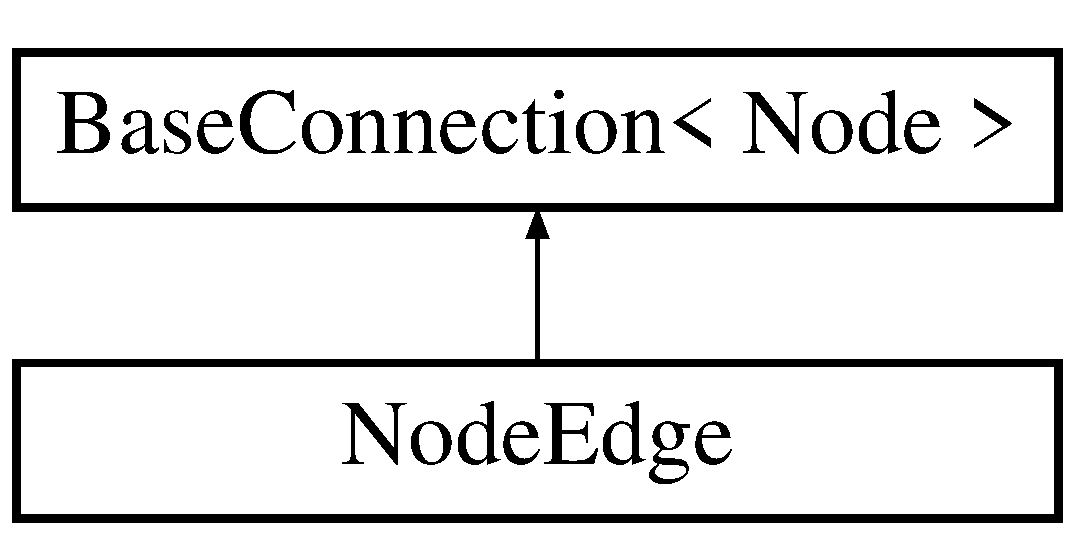
\includegraphics[height=2.000000cm]{class_node_edge}
\end{center}
\end{figure}
\subsection*{Public Member Functions}
\begin{DoxyCompactItemize}
\item 
\mbox{\hyperlink{class_node_edge_ae99d0852e1477a08c220aadde2a800ff}{Node\+Edge}} (\mbox{\hyperlink{class_node}{Node}} from, \mbox{\hyperlink{class_node}{Node}} to)
\item 
override float \mbox{\hyperlink{class_node_edge_aa2eb53bd74c21ecc54af55568af1b6cc}{Get\+Cost}} ()
\begin{DoxyCompactList}\small\item\em Returns the non-\/negative cost of the connection \end{DoxyCompactList}\end{DoxyCompactItemize}
\subsection*{Additional Inherited Members}


\subsection{Constructor \& Destructor Documentation}
\mbox{\Hypertarget{class_node_edge_ae99d0852e1477a08c220aadde2a800ff}\label{class_node_edge_ae99d0852e1477a08c220aadde2a800ff}} 
\index{Node\+Edge@{Node\+Edge}!Node\+Edge@{Node\+Edge}}
\index{Node\+Edge@{Node\+Edge}!Node\+Edge@{Node\+Edge}}
\subsubsection{\texorpdfstring{Node\+Edge()}{NodeEdge()}}
{\footnotesize\ttfamily Node\+Edge.\+Node\+Edge (\begin{DoxyParamCaption}\item[{\mbox{\hyperlink{class_node}{Node}}}]{from,  }\item[{\mbox{\hyperlink{class_node}{Node}}}]{to }\end{DoxyParamCaption})}



\subsection{Member Function Documentation}
\mbox{\Hypertarget{class_node_edge_aa2eb53bd74c21ecc54af55568af1b6cc}\label{class_node_edge_aa2eb53bd74c21ecc54af55568af1b6cc}} 
\index{Node\+Edge@{Node\+Edge}!Get\+Cost@{Get\+Cost}}
\index{Get\+Cost@{Get\+Cost}!Node\+Edge@{Node\+Edge}}
\subsubsection{\texorpdfstring{Get\+Cost()}{GetCost()}}
{\footnotesize\ttfamily override float Node\+Edge.\+Get\+Cost (\begin{DoxyParamCaption}{ }\end{DoxyParamCaption})\hspace{0.3cm}{\ttfamily [virtual]}}



Returns the non-\/negative cost of the connection 

\begin{DoxyReturn}{Returns}

\end{DoxyReturn}


Reimplemented from \mbox{\hyperlink{class_base_connection_a3f2351e9bf997450cca8f64e1e32337a}{Base\+Connection$<$ Node $>$}}.



The documentation for this class was generated from the following file\+:\begin{DoxyCompactItemize}
\item 
/\+Users/sabienambrose/\+Documents/\+Coding/\+Unity\+Mechanical\+Turk/\+Mechanical\+Turk/\+Assets/\+Scripts/\+Util/\+Containers/\+Graphs/\+Grids/\mbox{\hyperlink{_node_edge_8cs}{Node\+Edge.\+cs}}\end{DoxyCompactItemize}

\hypertarget{struct_noise_data}{}\section{Noise\+Data Struct Reference}
\label{struct_noise_data}\index{Noise\+Data@{Noise\+Data}}
\subsection*{Public Attributes}
\begin{DoxyCompactItemize}
\item 
float \mbox{[},\mbox{]} \mbox{\hyperlink{struct_noise_data_a17fa4f41e75b96ad3ae8b1459ab305aa}{noise\+Map}}
\item 
float \mbox{\hyperlink{struct_noise_data_ae3d28ea7c4a4fa91bd5a75b34ef103cc}{height\+Multiplier}}
\end{DoxyCompactItemize}


\subsection{Member Data Documentation}
\mbox{\Hypertarget{struct_noise_data_ae3d28ea7c4a4fa91bd5a75b34ef103cc}\label{struct_noise_data_ae3d28ea7c4a4fa91bd5a75b34ef103cc}} 
\index{Noise\+Data@{Noise\+Data}!height\+Multiplier@{height\+Multiplier}}
\index{height\+Multiplier@{height\+Multiplier}!Noise\+Data@{Noise\+Data}}
\subsubsection{\texorpdfstring{height\+Multiplier}{heightMultiplier}}
{\footnotesize\ttfamily float Noise\+Data.\+height\+Multiplier}

\mbox{\Hypertarget{struct_noise_data_a17fa4f41e75b96ad3ae8b1459ab305aa}\label{struct_noise_data_a17fa4f41e75b96ad3ae8b1459ab305aa}} 
\index{Noise\+Data@{Noise\+Data}!noise\+Map@{noise\+Map}}
\index{noise\+Map@{noise\+Map}!Noise\+Data@{Noise\+Data}}
\subsubsection{\texorpdfstring{noise\+Map}{noiseMap}}
{\footnotesize\ttfamily float \mbox{[},\mbox{]} Noise\+Data.\+noise\+Map}



The documentation for this struct was generated from the following file\+:\begin{DoxyCompactItemize}
\item 
/\+Users/sabienambrose/\+Documents/\+Coding/\+Unity\+Mechanical\+Turk/\+Mechanical\+Turk/\+Assets/\+Scripts/\+Generation/\mbox{\hyperlink{_noise_data_8cs}{Noise\+Data.\+cs}}\end{DoxyCompactItemize}

\hypertarget{class_noise_generator}{}\section{Noise\+Generator Class Reference}
\label{class_noise_generator}\index{Noise\+Generator@{Noise\+Generator}}
Inheritance diagram for Noise\+Generator\+:\begin{figure}[H]
\begin{center}
\leavevmode
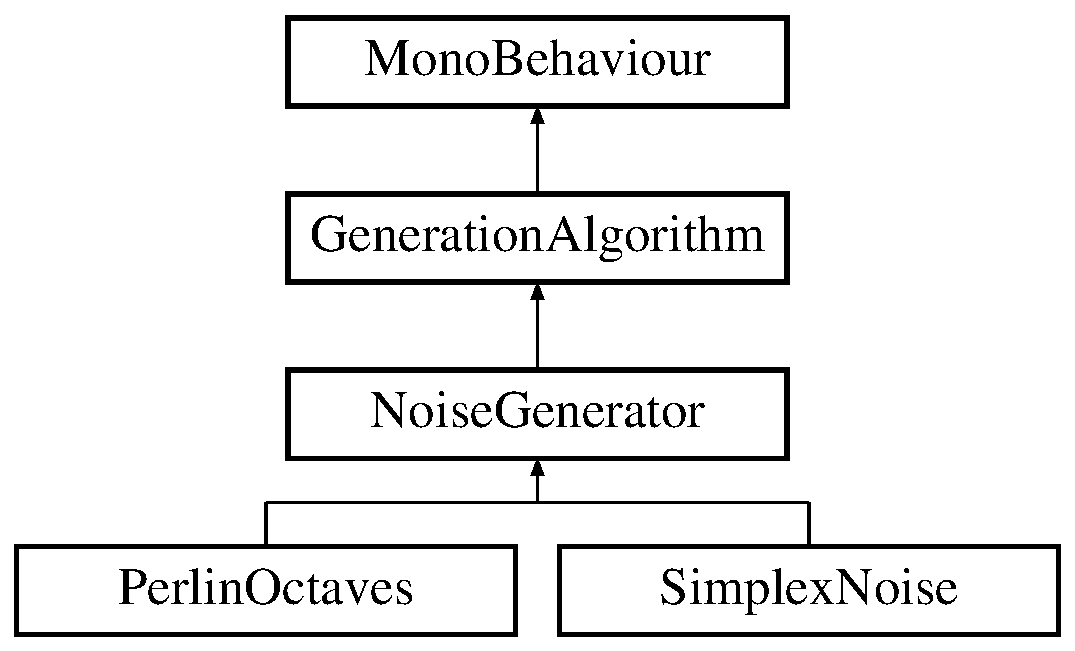
\includegraphics[height=4.000000cm]{class_noise_generator}
\end{center}
\end{figure}
\subsection*{Public Member Functions}
\begin{DoxyCompactItemize}
\item 
override void \mbox{\hyperlink{class_noise_generator_ad87355d424b537a1a4065d525ec18400}{Setup}} ()
\begin{DoxyCompactList}\small\item\em Collects any prerequisites for generation. \end{DoxyCompactList}\item 
override bool \mbox{\hyperlink{class_noise_generator_a9f6eefc7403c8d228dc1752086e8c745}{Can\+Generate}} ()
\begin{DoxyCompactList}\small\item\em Checks to see if generation prerequisites are met. \end{DoxyCompactList}\item 
override void \mbox{\hyperlink{class_noise_generator_af97b78b12d39a0ae2d05e1d28c970005}{Generate}} ()
\item 
abstract float \mbox{[},\mbox{]} \mbox{\hyperlink{class_noise_generator_a1d3983a9ad33c2734f373e9f2d8f13d7}{Generate\+Height\+Map}} (int map\+Width, int map\+Height)
\end{DoxyCompactItemize}
\subsection*{Public Attributes}
\begin{DoxyCompactItemize}
\item 
\mbox{\hyperlink{class_noise_map}{Noise\+Map}} \mbox{\hyperlink{class_noise_generator_a19e92d7669706bdd2cae8229dc6331f4}{noise\+Map}}
\item 
float \mbox{\hyperlink{class_noise_generator_a411009c00c7e62e99dccd0dd3b98c661}{scale}} = 1f
\end{DoxyCompactItemize}
\subsection*{Properties}
\begin{DoxyCompactItemize}
\item 
int \mbox{\hyperlink{class_noise_generator_abf59a5335539de9b8a38feca31f8ffe5}{width}}\hspace{0.3cm}{\ttfamily  \mbox{[}get, set\mbox{]}}
\item 
int \mbox{\hyperlink{class_noise_generator_a73fd14bf579ffcf3118b81be3107c0d5}{height}}\hspace{0.3cm}{\ttfamily  \mbox{[}get, set\mbox{]}}
\end{DoxyCompactItemize}


\subsection{Member Function Documentation}
\mbox{\Hypertarget{class_noise_generator_a9f6eefc7403c8d228dc1752086e8c745}\label{class_noise_generator_a9f6eefc7403c8d228dc1752086e8c745}} 
\index{Noise\+Generator@{Noise\+Generator}!Can\+Generate@{Can\+Generate}}
\index{Can\+Generate@{Can\+Generate}!Noise\+Generator@{Noise\+Generator}}
\subsubsection{\texorpdfstring{Can\+Generate()}{CanGenerate()}}
{\footnotesize\ttfamily override bool Noise\+Generator.\+Can\+Generate (\begin{DoxyParamCaption}{ }\end{DoxyParamCaption})\hspace{0.3cm}{\ttfamily [virtual]}}



Checks to see if generation prerequisites are met. 

\begin{DoxyReturn}{Returns}
true if ready for generation.
\end{DoxyReturn}


Implements \mbox{\hyperlink{class_generation_algorithm_af7d03e24e3b7fecfe2ae43f06915986d}{Generation\+Algorithm}}.

\mbox{\Hypertarget{class_noise_generator_af97b78b12d39a0ae2d05e1d28c970005}\label{class_noise_generator_af97b78b12d39a0ae2d05e1d28c970005}} 
\index{Noise\+Generator@{Noise\+Generator}!Generate@{Generate}}
\index{Generate@{Generate}!Noise\+Generator@{Noise\+Generator}}
\subsubsection{\texorpdfstring{Generate()}{Generate()}}
{\footnotesize\ttfamily override void Noise\+Generator.\+Generate (\begin{DoxyParamCaption}{ }\end{DoxyParamCaption})\hspace{0.3cm}{\ttfamily [virtual]}}



Implements \mbox{\hyperlink{class_generation_algorithm_ac2df20f7751c1b480ab958791d5c7d41}{Generation\+Algorithm}}.

\mbox{\Hypertarget{class_noise_generator_a1d3983a9ad33c2734f373e9f2d8f13d7}\label{class_noise_generator_a1d3983a9ad33c2734f373e9f2d8f13d7}} 
\index{Noise\+Generator@{Noise\+Generator}!Generate\+Height\+Map@{Generate\+Height\+Map}}
\index{Generate\+Height\+Map@{Generate\+Height\+Map}!Noise\+Generator@{Noise\+Generator}}
\subsubsection{\texorpdfstring{Generate\+Height\+Map()}{GenerateHeightMap()}}
{\footnotesize\ttfamily abstract float \mbox{[},\mbox{]} Noise\+Generator.\+Generate\+Height\+Map (\begin{DoxyParamCaption}\item[{int}]{map\+Width,  }\item[{int}]{map\+Height }\end{DoxyParamCaption})\hspace{0.3cm}{\ttfamily [pure virtual]}}



Implemented in \mbox{\hyperlink{class_simplex_noise_aea5b04e1455da3c6eb8b29deb28a239c}{Simplex\+Noise}}, and \mbox{\hyperlink{class_perlin_octaves_ac5deb001801dbfe9666df3dea023ce7a}{Perlin\+Octaves}}.

\mbox{\Hypertarget{class_noise_generator_ad87355d424b537a1a4065d525ec18400}\label{class_noise_generator_ad87355d424b537a1a4065d525ec18400}} 
\index{Noise\+Generator@{Noise\+Generator}!Setup@{Setup}}
\index{Setup@{Setup}!Noise\+Generator@{Noise\+Generator}}
\subsubsection{\texorpdfstring{Setup()}{Setup()}}
{\footnotesize\ttfamily override void Noise\+Generator.\+Setup (\begin{DoxyParamCaption}{ }\end{DoxyParamCaption})\hspace{0.3cm}{\ttfamily [virtual]}}



Collects any prerequisites for generation. 



Implements \mbox{\hyperlink{class_generation_algorithm_a5e891b08f0c1d8f4ccc9ad06667691ec}{Generation\+Algorithm}}.



Reimplemented in \mbox{\hyperlink{class_simplex_noise_a43164ec5960921789ce75e83651717cf}{Simplex\+Noise}}.



\subsection{Member Data Documentation}
\mbox{\Hypertarget{class_noise_generator_a19e92d7669706bdd2cae8229dc6331f4}\label{class_noise_generator_a19e92d7669706bdd2cae8229dc6331f4}} 
\index{Noise\+Generator@{Noise\+Generator}!noise\+Map@{noise\+Map}}
\index{noise\+Map@{noise\+Map}!Noise\+Generator@{Noise\+Generator}}
\subsubsection{\texorpdfstring{noise\+Map}{noiseMap}}
{\footnotesize\ttfamily \mbox{\hyperlink{class_noise_map}{Noise\+Map}} Noise\+Generator.\+noise\+Map}

\mbox{\Hypertarget{class_noise_generator_a411009c00c7e62e99dccd0dd3b98c661}\label{class_noise_generator_a411009c00c7e62e99dccd0dd3b98c661}} 
\index{Noise\+Generator@{Noise\+Generator}!scale@{scale}}
\index{scale@{scale}!Noise\+Generator@{Noise\+Generator}}
\subsubsection{\texorpdfstring{scale}{scale}}
{\footnotesize\ttfamily float Noise\+Generator.\+scale = 1f}



\subsection{Property Documentation}
\mbox{\Hypertarget{class_noise_generator_a73fd14bf579ffcf3118b81be3107c0d5}\label{class_noise_generator_a73fd14bf579ffcf3118b81be3107c0d5}} 
\index{Noise\+Generator@{Noise\+Generator}!height@{height}}
\index{height@{height}!Noise\+Generator@{Noise\+Generator}}
\subsubsection{\texorpdfstring{height}{height}}
{\footnotesize\ttfamily int Noise\+Generator.\+height\hspace{0.3cm}{\ttfamily [get]}, {\ttfamily [set]}}

\mbox{\Hypertarget{class_noise_generator_abf59a5335539de9b8a38feca31f8ffe5}\label{class_noise_generator_abf59a5335539de9b8a38feca31f8ffe5}} 
\index{Noise\+Generator@{Noise\+Generator}!width@{width}}
\index{width@{width}!Noise\+Generator@{Noise\+Generator}}
\subsubsection{\texorpdfstring{width}{width}}
{\footnotesize\ttfamily int Noise\+Generator.\+width\hspace{0.3cm}{\ttfamily [get]}, {\ttfamily [set]}}



The documentation for this class was generated from the following file\+:\begin{DoxyCompactItemize}
\item 
/\+Users/sabienambrose/\+Documents/\+Coding/\+Unity\+Mechanical\+Turk/\+Mechanical\+Turk/\+Assets/\+Scripts/\+Framework/\+Generation/\mbox{\hyperlink{_noise_generator_8cs}{Noise\+Generator.\+cs}}\end{DoxyCompactItemize}

\hypertarget{class_noise_map}{}\section{Noise\+Map Class Reference}
\label{class_noise_map}\index{Noise\+Map@{Noise\+Map}}


2D Array with indexers  


Inheritance diagram for Noise\+Map\+:\begin{figure}[H]
\begin{center}
\leavevmode
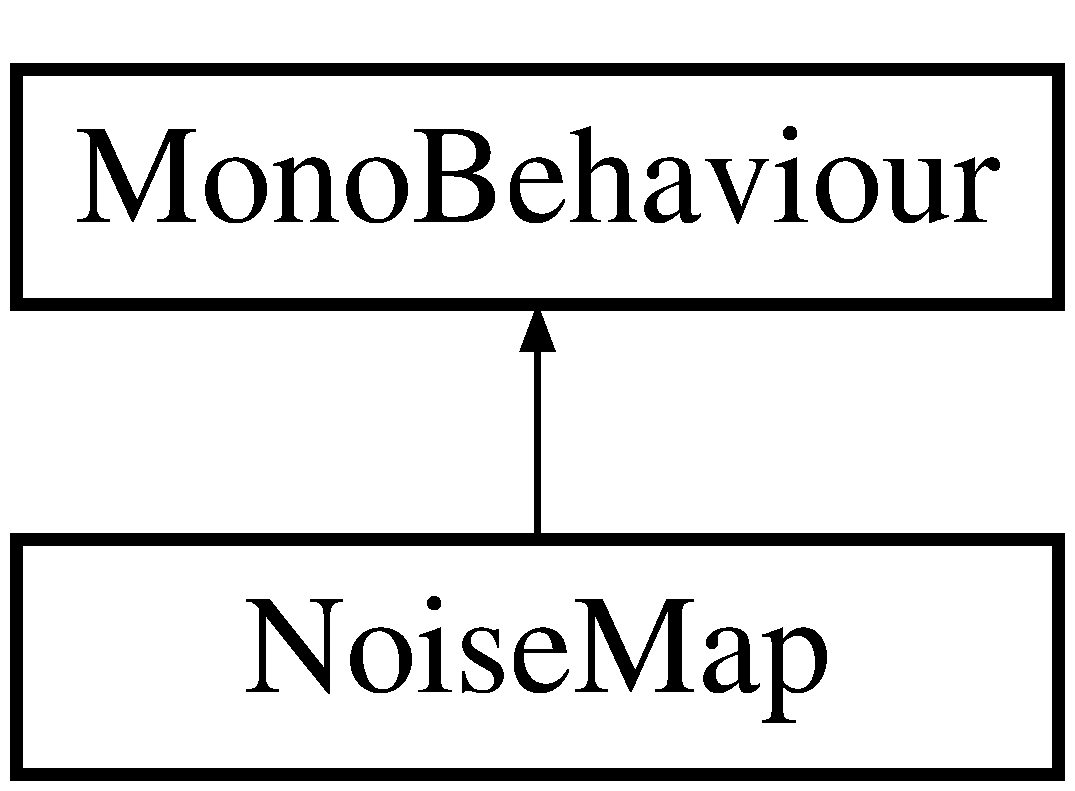
\includegraphics[height=2.000000cm]{class_noise_map}
\end{center}
\end{figure}
\subsection*{Public Member Functions}
\begin{DoxyCompactItemize}
\item 
void \mbox{\hyperlink{class_noise_map_a202d577f21b8d8264ffe78cea2149cb8}{Resize}} (Vector2\+Int new\+Size)
\item 
int \mbox{\hyperlink{class_noise_map_a833fc31b1d8e9792634f22e74f099625}{To\+Index}} (int x, int y)
\item 
int \mbox{\hyperlink{class_noise_map_af3cba5e8724a9234b800836ed242e9aa}{Get\+Width}} ()
\item 
int \mbox{\hyperlink{class_noise_map_a786377605734c7aec5c73905e0099780}{Get\+Height}} ()
\end{DoxyCompactItemize}
\subsection*{Properties}
\begin{DoxyCompactItemize}
\item 
Vector2\+Int \mbox{\hyperlink{class_noise_map_aaa73317c8c0de24d323bd652fb93faee}{Dimensions}}\hspace{0.3cm}{\ttfamily  \mbox{[}get, set\mbox{]}}
\item 
int \mbox{\hyperlink{class_noise_map_a0acc0f92acd8a77e9058c8ca446cf00a}{Width}}\hspace{0.3cm}{\ttfamily  \mbox{[}get, set\mbox{]}}
\item 
int \mbox{\hyperlink{class_noise_map_af65841f7300d8b15bf3c6006246fca9e}{Height}}\hspace{0.3cm}{\ttfamily  \mbox{[}get, set\mbox{]}}
\item 
float \mbox{[},\mbox{]} \mbox{\hyperlink{class_noise_map_a9ee9185c988152a2989feab0683ac664}{Values}}\hspace{0.3cm}{\ttfamily  \mbox{[}get, set\mbox{]}}
\item 
float \mbox{\hyperlink{class_noise_map_a83be172bbaf8fcaad7bcc6b3b1ad9dbd}{this\mbox{[}int i\mbox{]}}}\hspace{0.3cm}{\ttfamily  \mbox{[}get, set\mbox{]}}
\item 
float \mbox{\hyperlink{class_noise_map_aa0f8f5462a066a14667ea1269edc33bd}{this\mbox{[}\+Vector2\+Int v2\mbox{]}}}\hspace{0.3cm}{\ttfamily  \mbox{[}get, set\mbox{]}}
\item 
float \mbox{\hyperlink{class_noise_map_aa32ffbd1bf29cf414b65e195dae5c221}{this\mbox{[}int x, int y\mbox{]}}}\hspace{0.3cm}{\ttfamily  \mbox{[}get, set\mbox{]}}
\end{DoxyCompactItemize}


\subsection{Detailed Description}
2D Array with indexers 



\subsection{Member Function Documentation}
\mbox{\Hypertarget{class_noise_map_a786377605734c7aec5c73905e0099780}\label{class_noise_map_a786377605734c7aec5c73905e0099780}} 
\index{Noise\+Map@{Noise\+Map}!Get\+Height@{Get\+Height}}
\index{Get\+Height@{Get\+Height}!Noise\+Map@{Noise\+Map}}
\subsubsection{\texorpdfstring{Get\+Height()}{GetHeight()}}
{\footnotesize\ttfamily int Noise\+Map.\+Get\+Height (\begin{DoxyParamCaption}{ }\end{DoxyParamCaption})}

\mbox{\Hypertarget{class_noise_map_af3cba5e8724a9234b800836ed242e9aa}\label{class_noise_map_af3cba5e8724a9234b800836ed242e9aa}} 
\index{Noise\+Map@{Noise\+Map}!Get\+Width@{Get\+Width}}
\index{Get\+Width@{Get\+Width}!Noise\+Map@{Noise\+Map}}
\subsubsection{\texorpdfstring{Get\+Width()}{GetWidth()}}
{\footnotesize\ttfamily int Noise\+Map.\+Get\+Width (\begin{DoxyParamCaption}{ }\end{DoxyParamCaption})}

\mbox{\Hypertarget{class_noise_map_a202d577f21b8d8264ffe78cea2149cb8}\label{class_noise_map_a202d577f21b8d8264ffe78cea2149cb8}} 
\index{Noise\+Map@{Noise\+Map}!Resize@{Resize}}
\index{Resize@{Resize}!Noise\+Map@{Noise\+Map}}
\subsubsection{\texorpdfstring{Resize()}{Resize()}}
{\footnotesize\ttfamily void Noise\+Map.\+Resize (\begin{DoxyParamCaption}\item[{Vector2\+Int}]{new\+Size }\end{DoxyParamCaption})}

\mbox{\Hypertarget{class_noise_map_a833fc31b1d8e9792634f22e74f099625}\label{class_noise_map_a833fc31b1d8e9792634f22e74f099625}} 
\index{Noise\+Map@{Noise\+Map}!To\+Index@{To\+Index}}
\index{To\+Index@{To\+Index}!Noise\+Map@{Noise\+Map}}
\subsubsection{\texorpdfstring{To\+Index()}{ToIndex()}}
{\footnotesize\ttfamily int Noise\+Map.\+To\+Index (\begin{DoxyParamCaption}\item[{int}]{x,  }\item[{int}]{y }\end{DoxyParamCaption})}



\subsection{Property Documentation}
\mbox{\Hypertarget{class_noise_map_aaa73317c8c0de24d323bd652fb93faee}\label{class_noise_map_aaa73317c8c0de24d323bd652fb93faee}} 
\index{Noise\+Map@{Noise\+Map}!Dimensions@{Dimensions}}
\index{Dimensions@{Dimensions}!Noise\+Map@{Noise\+Map}}
\subsubsection{\texorpdfstring{Dimensions}{Dimensions}}
{\footnotesize\ttfamily Vector2\+Int Noise\+Map.\+Dimensions\hspace{0.3cm}{\ttfamily [get]}, {\ttfamily [set]}}

\mbox{\Hypertarget{class_noise_map_af65841f7300d8b15bf3c6006246fca9e}\label{class_noise_map_af65841f7300d8b15bf3c6006246fca9e}} 
\index{Noise\+Map@{Noise\+Map}!Height@{Height}}
\index{Height@{Height}!Noise\+Map@{Noise\+Map}}
\subsubsection{\texorpdfstring{Height}{Height}}
{\footnotesize\ttfamily int Noise\+Map.\+Height\hspace{0.3cm}{\ttfamily [get]}, {\ttfamily [set]}}

\mbox{\Hypertarget{class_noise_map_a83be172bbaf8fcaad7bcc6b3b1ad9dbd}\label{class_noise_map_a83be172bbaf8fcaad7bcc6b3b1ad9dbd}} 
\index{Noise\+Map@{Noise\+Map}!this\mbox{[}int i\mbox{]}@{this[int i]}}
\index{this\mbox{[}int i\mbox{]}@{this[int i]}!Noise\+Map@{Noise\+Map}}
\subsubsection{\texorpdfstring{this[int i]}{this[int i]}}
{\footnotesize\ttfamily float Noise\+Map.\+this\mbox{[}int i\mbox{]}\hspace{0.3cm}{\ttfamily [get]}, {\ttfamily [set]}}

\mbox{\Hypertarget{class_noise_map_aa32ffbd1bf29cf414b65e195dae5c221}\label{class_noise_map_aa32ffbd1bf29cf414b65e195dae5c221}} 
\index{Noise\+Map@{Noise\+Map}!this\mbox{[}int x, int y\mbox{]}@{this[int x, int y]}}
\index{this\mbox{[}int x, int y\mbox{]}@{this[int x, int y]}!Noise\+Map@{Noise\+Map}}
\subsubsection{\texorpdfstring{this[int x, int y]}{this[int x, int y]}}
{\footnotesize\ttfamily float Noise\+Map.\+this\mbox{[}int x, int y\mbox{]}\hspace{0.3cm}{\ttfamily [get]}, {\ttfamily [set]}}

\mbox{\Hypertarget{class_noise_map_aa0f8f5462a066a14667ea1269edc33bd}\label{class_noise_map_aa0f8f5462a066a14667ea1269edc33bd}} 
\index{Noise\+Map@{Noise\+Map}!this\mbox{[}\+Vector2\+Int v2\mbox{]}@{this[Vector2\+Int v2]}}
\index{this\mbox{[}\+Vector2\+Int v2\mbox{]}@{this[Vector2\+Int v2]}!Noise\+Map@{Noise\+Map}}
\subsubsection{\texorpdfstring{this[Vector2\+Int v2]}{this[Vector2Int v2]}}
{\footnotesize\ttfamily float Noise\+Map.\+this\mbox{[}Vector2\+Int v2\mbox{]}\hspace{0.3cm}{\ttfamily [get]}, {\ttfamily [set]}}

\mbox{\Hypertarget{class_noise_map_a9ee9185c988152a2989feab0683ac664}\label{class_noise_map_a9ee9185c988152a2989feab0683ac664}} 
\index{Noise\+Map@{Noise\+Map}!Values@{Values}}
\index{Values@{Values}!Noise\+Map@{Noise\+Map}}
\subsubsection{\texorpdfstring{Values}{Values}}
{\footnotesize\ttfamily float \mbox{[},\mbox{]} Noise\+Map.\+Values\hspace{0.3cm}{\ttfamily [get]}, {\ttfamily [set]}}

\mbox{\Hypertarget{class_noise_map_a0acc0f92acd8a77e9058c8ca446cf00a}\label{class_noise_map_a0acc0f92acd8a77e9058c8ca446cf00a}} 
\index{Noise\+Map@{Noise\+Map}!Width@{Width}}
\index{Width@{Width}!Noise\+Map@{Noise\+Map}}
\subsubsection{\texorpdfstring{Width}{Width}}
{\footnotesize\ttfamily int Noise\+Map.\+Width\hspace{0.3cm}{\ttfamily [get]}, {\ttfamily [set]}}



The documentation for this class was generated from the following file\+:\begin{DoxyCompactItemize}
\item 
/\+Users/sabienambrose/\+Documents/\+Coding/\+Unity\+Mechanical\+Turk/\+Mechanical\+Turk/\+Assets/\+Scripts/\+Util/\+Containers/\mbox{\hyperlink{_noise_map_8cs}{Noise\+Map.\+cs}}\end{DoxyCompactItemize}

\hypertarget{class_object_picker}{}\section{Object\+Picker Class Reference}
\label{class_object_picker}\index{Object\+Picker@{Object\+Picker}}
Inheritance diagram for Object\+Picker\+:\begin{figure}[H]
\begin{center}
\leavevmode
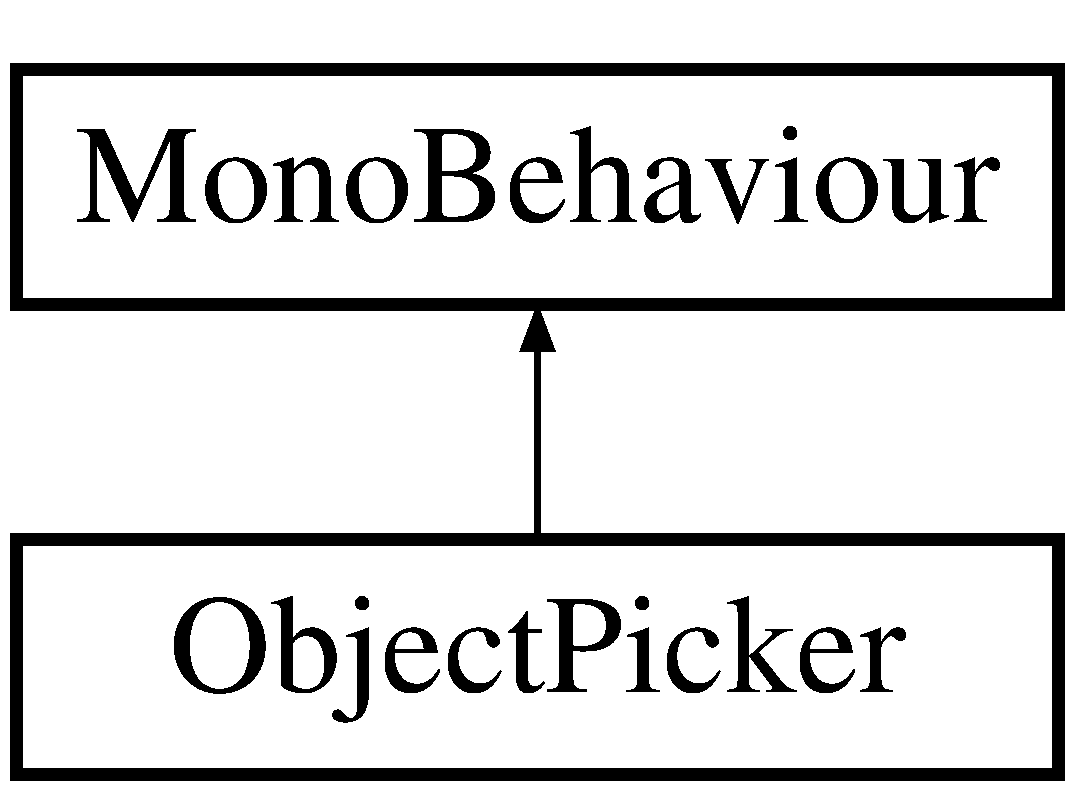
\includegraphics[height=2.000000cm]{class_object_picker}
\end{center}
\end{figure}
\subsection*{Public Member Functions}
\begin{DoxyCompactItemize}
\item 
abstract Game\+Object \mbox{[}$\,$\mbox{]} \mbox{\hyperlink{class_object_picker_a637528ecd5f6814b693809aa01c73d0d}{Get\+Object\+Options}} ()
\item 
virtual Game\+Object \mbox{\hyperlink{class_object_picker_af46555e63096c06e8148294c71d29ae0}{Get\+Choice}} (\mbox{\hyperlink{_object_picker_8cs_a2dcef18caa6de91171bf235b9189206d}{Selection\+Method}} selection\+Method)
\item 
virtual Game\+Object \mbox{\hyperlink{class_object_picker_ae93cde0e42852dcbe39015206c70cfd5}{Get\+Choice}} ()
\item 
virtual Game\+Object \mbox{\hyperlink{class_object_picker_a50bda66bcb02e806964805423327d6d7}{Get\+Random\+Choice}} ()
\item 
abstract Game\+Object \mbox{\hyperlink{class_object_picker_aeb1c11e83af3c5e6b76a431af437ff40}{Get\+Min\+Util\+Choice}} ()
\item 
abstract Game\+Object \mbox{\hyperlink{class_object_picker_a22f1eaaa6cc1c7b545f0fb5c369fc445}{Get\+Max\+Util\+Choice}} ()
\end{DoxyCompactItemize}
\subsection*{Public Attributes}
\begin{DoxyCompactItemize}
\item 
\mbox{\hyperlink{_object_picker_8cs_a2dcef18caa6de91171bf235b9189206d}{Selection\+Method}} \mbox{\hyperlink{class_object_picker_a111abafc332a892a7155c876329e08f3}{default\+Selection\+Method}}
\end{DoxyCompactItemize}


\subsection{Member Function Documentation}
\mbox{\Hypertarget{class_object_picker_af46555e63096c06e8148294c71d29ae0}\label{class_object_picker_af46555e63096c06e8148294c71d29ae0}} 
\index{Object\+Picker@{Object\+Picker}!Get\+Choice@{Get\+Choice}}
\index{Get\+Choice@{Get\+Choice}!Object\+Picker@{Object\+Picker}}
\subsubsection{\texorpdfstring{Get\+Choice()}{GetChoice()}\hspace{0.1cm}{\footnotesize\ttfamily [1/2]}}
{\footnotesize\ttfamily virtual Game\+Object Object\+Picker.\+Get\+Choice (\begin{DoxyParamCaption}\item[{\mbox{\hyperlink{_object_picker_8cs_a2dcef18caa6de91171bf235b9189206d}{Selection\+Method}}}]{selection\+Method }\end{DoxyParamCaption})\hspace{0.3cm}{\ttfamily [virtual]}}

\mbox{\Hypertarget{class_object_picker_ae93cde0e42852dcbe39015206c70cfd5}\label{class_object_picker_ae93cde0e42852dcbe39015206c70cfd5}} 
\index{Object\+Picker@{Object\+Picker}!Get\+Choice@{Get\+Choice}}
\index{Get\+Choice@{Get\+Choice}!Object\+Picker@{Object\+Picker}}
\subsubsection{\texorpdfstring{Get\+Choice()}{GetChoice()}\hspace{0.1cm}{\footnotesize\ttfamily [2/2]}}
{\footnotesize\ttfamily virtual Game\+Object Object\+Picker.\+Get\+Choice (\begin{DoxyParamCaption}{ }\end{DoxyParamCaption})\hspace{0.3cm}{\ttfamily [virtual]}}

\mbox{\Hypertarget{class_object_picker_a22f1eaaa6cc1c7b545f0fb5c369fc445}\label{class_object_picker_a22f1eaaa6cc1c7b545f0fb5c369fc445}} 
\index{Object\+Picker@{Object\+Picker}!Get\+Max\+Util\+Choice@{Get\+Max\+Util\+Choice}}
\index{Get\+Max\+Util\+Choice@{Get\+Max\+Util\+Choice}!Object\+Picker@{Object\+Picker}}
\subsubsection{\texorpdfstring{Get\+Max\+Util\+Choice()}{GetMaxUtilChoice()}}
{\footnotesize\ttfamily abstract Game\+Object Object\+Picker.\+Get\+Max\+Util\+Choice (\begin{DoxyParamCaption}{ }\end{DoxyParamCaption})\hspace{0.3cm}{\ttfamily [pure virtual]}}

\mbox{\Hypertarget{class_object_picker_aeb1c11e83af3c5e6b76a431af437ff40}\label{class_object_picker_aeb1c11e83af3c5e6b76a431af437ff40}} 
\index{Object\+Picker@{Object\+Picker}!Get\+Min\+Util\+Choice@{Get\+Min\+Util\+Choice}}
\index{Get\+Min\+Util\+Choice@{Get\+Min\+Util\+Choice}!Object\+Picker@{Object\+Picker}}
\subsubsection{\texorpdfstring{Get\+Min\+Util\+Choice()}{GetMinUtilChoice()}}
{\footnotesize\ttfamily abstract Game\+Object Object\+Picker.\+Get\+Min\+Util\+Choice (\begin{DoxyParamCaption}{ }\end{DoxyParamCaption})\hspace{0.3cm}{\ttfamily [pure virtual]}}

\mbox{\Hypertarget{class_object_picker_a637528ecd5f6814b693809aa01c73d0d}\label{class_object_picker_a637528ecd5f6814b693809aa01c73d0d}} 
\index{Object\+Picker@{Object\+Picker}!Get\+Object\+Options@{Get\+Object\+Options}}
\index{Get\+Object\+Options@{Get\+Object\+Options}!Object\+Picker@{Object\+Picker}}
\subsubsection{\texorpdfstring{Get\+Object\+Options()}{GetObjectOptions()}}
{\footnotesize\ttfamily abstract Game\+Object \mbox{[}$\,$\mbox{]} Object\+Picker.\+Get\+Object\+Options (\begin{DoxyParamCaption}{ }\end{DoxyParamCaption})\hspace{0.3cm}{\ttfamily [pure virtual]}}

\mbox{\Hypertarget{class_object_picker_a50bda66bcb02e806964805423327d6d7}\label{class_object_picker_a50bda66bcb02e806964805423327d6d7}} 
\index{Object\+Picker@{Object\+Picker}!Get\+Random\+Choice@{Get\+Random\+Choice}}
\index{Get\+Random\+Choice@{Get\+Random\+Choice}!Object\+Picker@{Object\+Picker}}
\subsubsection{\texorpdfstring{Get\+Random\+Choice()}{GetRandomChoice()}}
{\footnotesize\ttfamily virtual Game\+Object Object\+Picker.\+Get\+Random\+Choice (\begin{DoxyParamCaption}{ }\end{DoxyParamCaption})\hspace{0.3cm}{\ttfamily [virtual]}}



\subsection{Member Data Documentation}
\mbox{\Hypertarget{class_object_picker_a111abafc332a892a7155c876329e08f3}\label{class_object_picker_a111abafc332a892a7155c876329e08f3}} 
\index{Object\+Picker@{Object\+Picker}!default\+Selection\+Method@{default\+Selection\+Method}}
\index{default\+Selection\+Method@{default\+Selection\+Method}!Object\+Picker@{Object\+Picker}}
\subsubsection{\texorpdfstring{default\+Selection\+Method}{defaultSelectionMethod}}
{\footnotesize\ttfamily \mbox{\hyperlink{_object_picker_8cs_a2dcef18caa6de91171bf235b9189206d}{Selection\+Method}} Object\+Picker.\+default\+Selection\+Method}



The documentation for this class was generated from the following file\+:\begin{DoxyCompactItemize}
\item 
/\+Users/sabienambrose/\+Documents/\+Coding/\+Unity\+Mechanical\+Turk/\+Mechanical\+Turk/\+Assets/\+Scripts/\+Framework/\+Generation/\mbox{\hyperlink{_object_picker_8cs}{Object\+Picker.\+cs}}\end{DoxyCompactItemize}

\hypertarget{class_path_following}{}\section{Path\+Following Class Reference}
\label{class_path_following}\index{Path\+Following@{Path\+Following}}
Inheritance diagram for Path\+Following\+:\begin{figure}[H]
\begin{center}
\leavevmode
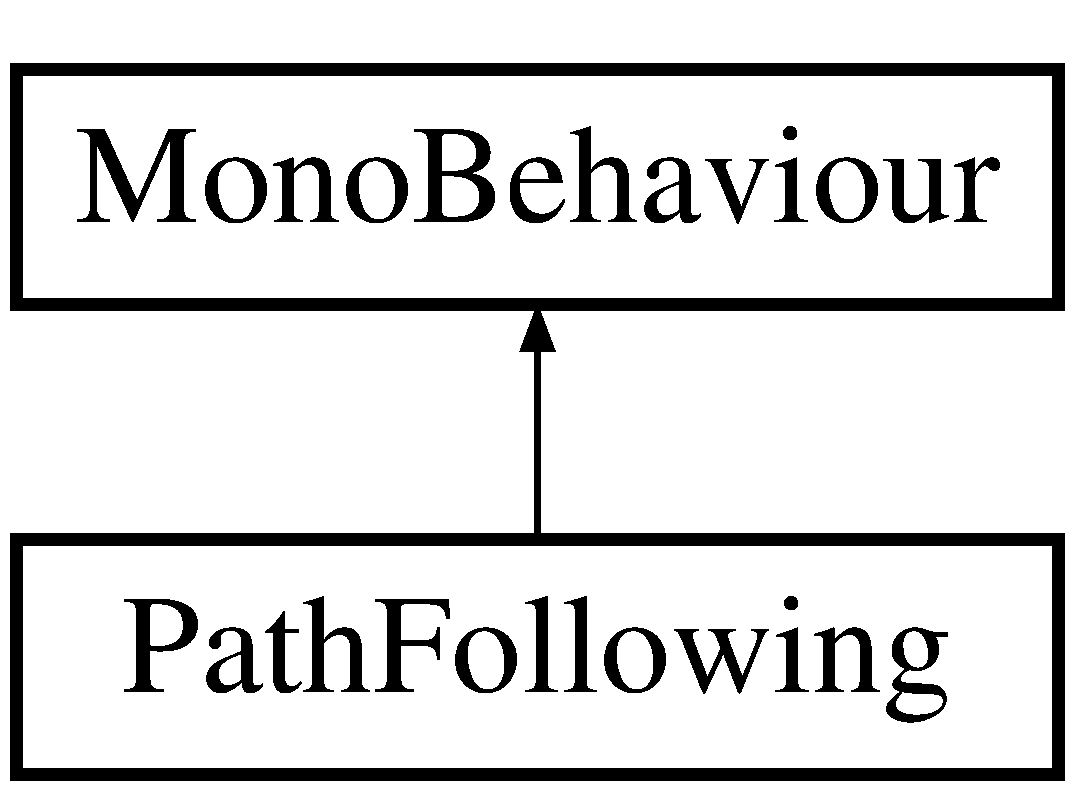
\includegraphics[height=2.000000cm]{class_path_following}
\end{center}
\end{figure}
\subsection*{Public Member Functions}
\begin{DoxyCompactItemize}
\item 
void \mbox{\hyperlink{class_path_following_a2b80587b5939c9e6c4b8428c357ca6dd}{Start\+Path}} ()
\end{DoxyCompactItemize}
\subsection*{Public Attributes}
\begin{DoxyCompactItemize}
\item 
\mbox{\hyperlink{class_tile_a_star}{Tile\+A\+Star}} \mbox{\hyperlink{class_path_following_aebd9ee9093f350ad3ecc77b51e83910a}{path\+Finder}}
\item 
float \mbox{\hyperlink{class_path_following_a49b1482d4ff9c77a24e86d7cd05322c5}{speed}} = 0.\+5f
\item 
Transform \mbox{\hyperlink{class_path_following_a59519acae127788d7ed4d3a5aff64a82}{goal}}
\item 
List$<$ Vector3 $>$ \mbox{\hyperlink{class_path_following_ac4a4b53022913ec510ae0d6e63836151}{path}} = new List$<$Vector3$>$()
\item 
int \mbox{\hyperlink{class_path_following_abffab101a600ffd65d09044089a56352}{path\+Index}} = -\/1
\item 
float \mbox{\hyperlink{class_path_following_a04b81f97ff5a50de9e33fa06adb0b0e1}{acceptable\+Distance}} = 0.\+25f
\item 
bool \mbox{\hyperlink{class_path_following_ad8b5497dee6c46c8a3e37353c7f41cdf}{needs\+Path}} = true
\item 
bool \mbox{\hyperlink{class_path_following_ac9f0499d23632e1ebc46c69cea2c615b}{uses\+Smoothing}} = true
\item 
bool \mbox{\hyperlink{class_path_following_a070098fa92eeae99442f12c2af232b3e}{should\+Move}} = false
\end{DoxyCompactItemize}


\subsection{Member Function Documentation}
\mbox{\Hypertarget{class_path_following_a2b80587b5939c9e6c4b8428c357ca6dd}\label{class_path_following_a2b80587b5939c9e6c4b8428c357ca6dd}} 
\index{Path\+Following@{Path\+Following}!Start\+Path@{Start\+Path}}
\index{Start\+Path@{Start\+Path}!Path\+Following@{Path\+Following}}
\subsubsection{\texorpdfstring{Start\+Path()}{StartPath()}}
{\footnotesize\ttfamily void Path\+Following.\+Start\+Path (\begin{DoxyParamCaption}{ }\end{DoxyParamCaption})}



\subsection{Member Data Documentation}
\mbox{\Hypertarget{class_path_following_a04b81f97ff5a50de9e33fa06adb0b0e1}\label{class_path_following_a04b81f97ff5a50de9e33fa06adb0b0e1}} 
\index{Path\+Following@{Path\+Following}!acceptable\+Distance@{acceptable\+Distance}}
\index{acceptable\+Distance@{acceptable\+Distance}!Path\+Following@{Path\+Following}}
\subsubsection{\texorpdfstring{acceptable\+Distance}{acceptableDistance}}
{\footnotesize\ttfamily float Path\+Following.\+acceptable\+Distance = 0.\+25f}

\mbox{\Hypertarget{class_path_following_a59519acae127788d7ed4d3a5aff64a82}\label{class_path_following_a59519acae127788d7ed4d3a5aff64a82}} 
\index{Path\+Following@{Path\+Following}!goal@{goal}}
\index{goal@{goal}!Path\+Following@{Path\+Following}}
\subsubsection{\texorpdfstring{goal}{goal}}
{\footnotesize\ttfamily Transform Path\+Following.\+goal}

\mbox{\Hypertarget{class_path_following_ad8b5497dee6c46c8a3e37353c7f41cdf}\label{class_path_following_ad8b5497dee6c46c8a3e37353c7f41cdf}} 
\index{Path\+Following@{Path\+Following}!needs\+Path@{needs\+Path}}
\index{needs\+Path@{needs\+Path}!Path\+Following@{Path\+Following}}
\subsubsection{\texorpdfstring{needs\+Path}{needsPath}}
{\footnotesize\ttfamily bool Path\+Following.\+needs\+Path = true}

\mbox{\Hypertarget{class_path_following_ac4a4b53022913ec510ae0d6e63836151}\label{class_path_following_ac4a4b53022913ec510ae0d6e63836151}} 
\index{Path\+Following@{Path\+Following}!path@{path}}
\index{path@{path}!Path\+Following@{Path\+Following}}
\subsubsection{\texorpdfstring{path}{path}}
{\footnotesize\ttfamily List$<$Vector3$>$ Path\+Following.\+path = new List$<$Vector3$>$()}

\mbox{\Hypertarget{class_path_following_aebd9ee9093f350ad3ecc77b51e83910a}\label{class_path_following_aebd9ee9093f350ad3ecc77b51e83910a}} 
\index{Path\+Following@{Path\+Following}!path\+Finder@{path\+Finder}}
\index{path\+Finder@{path\+Finder}!Path\+Following@{Path\+Following}}
\subsubsection{\texorpdfstring{path\+Finder}{pathFinder}}
{\footnotesize\ttfamily \mbox{\hyperlink{class_tile_a_star}{Tile\+A\+Star}} Path\+Following.\+path\+Finder}

\mbox{\Hypertarget{class_path_following_abffab101a600ffd65d09044089a56352}\label{class_path_following_abffab101a600ffd65d09044089a56352}} 
\index{Path\+Following@{Path\+Following}!path\+Index@{path\+Index}}
\index{path\+Index@{path\+Index}!Path\+Following@{Path\+Following}}
\subsubsection{\texorpdfstring{path\+Index}{pathIndex}}
{\footnotesize\ttfamily int Path\+Following.\+path\+Index = -\/1}

\mbox{\Hypertarget{class_path_following_a070098fa92eeae99442f12c2af232b3e}\label{class_path_following_a070098fa92eeae99442f12c2af232b3e}} 
\index{Path\+Following@{Path\+Following}!should\+Move@{should\+Move}}
\index{should\+Move@{should\+Move}!Path\+Following@{Path\+Following}}
\subsubsection{\texorpdfstring{should\+Move}{shouldMove}}
{\footnotesize\ttfamily bool Path\+Following.\+should\+Move = false}

\mbox{\Hypertarget{class_path_following_a49b1482d4ff9c77a24e86d7cd05322c5}\label{class_path_following_a49b1482d4ff9c77a24e86d7cd05322c5}} 
\index{Path\+Following@{Path\+Following}!speed@{speed}}
\index{speed@{speed}!Path\+Following@{Path\+Following}}
\subsubsection{\texorpdfstring{speed}{speed}}
{\footnotesize\ttfamily float Path\+Following.\+speed = 0.\+5f}

\mbox{\Hypertarget{class_path_following_ac9f0499d23632e1ebc46c69cea2c615b}\label{class_path_following_ac9f0499d23632e1ebc46c69cea2c615b}} 
\index{Path\+Following@{Path\+Following}!uses\+Smoothing@{uses\+Smoothing}}
\index{uses\+Smoothing@{uses\+Smoothing}!Path\+Following@{Path\+Following}}
\subsubsection{\texorpdfstring{uses\+Smoothing}{usesSmoothing}}
{\footnotesize\ttfamily bool Path\+Following.\+uses\+Smoothing = true}



The documentation for this class was generated from the following file\+:\begin{DoxyCompactItemize}
\item 
/\+Users/sabienambrose/\+Documents/\+Coding/\+Unity\+Mechanical\+Turk/\+Mechanical\+Turk/\+Assets/\+Scripts/\+Pathfinding/\mbox{\hyperlink{_path_following_8cs}{Path\+Following.\+cs}}\end{DoxyCompactItemize}

\hypertarget{class_path_smoother}{}\section{Path\+Smoother Class Reference}
\label{class_path_smoother}\index{Path\+Smoother@{Path\+Smoother}}
Inheritance diagram for Path\+Smoother\+:\begin{figure}[H]
\begin{center}
\leavevmode
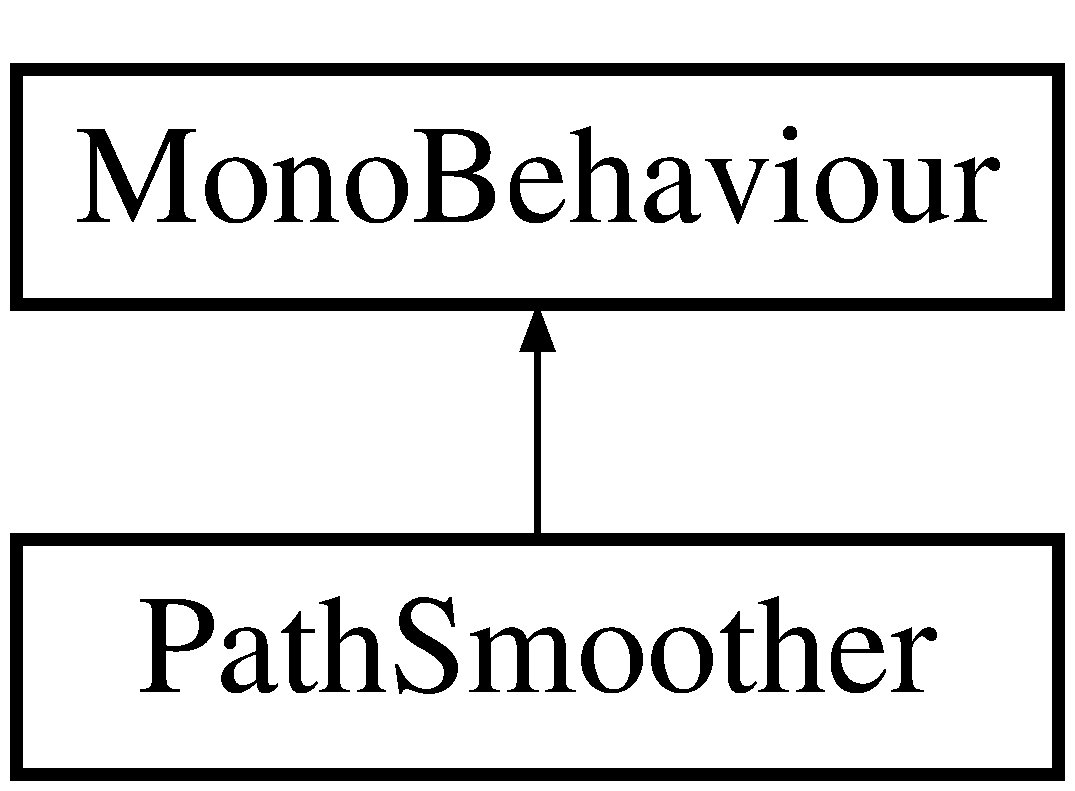
\includegraphics[height=2.000000cm]{class_path_smoother}
\end{center}
\end{figure}
\subsection*{Public Member Functions}
\begin{DoxyCompactItemize}
\item 
List$<$ Vector3 $>$ \mbox{\hyperlink{class_path_smoother_a415277dfe81500b7a69f3a28a6af24b9}{Smooth\+Path}} (List$<$ Vector3 $>$ input\+Path)
\begin{DoxyCompactList}\small\item\em Takes an input path made up of nodes and returns a smoothed output path. \end{DoxyCompactList}\end{DoxyCompactItemize}


\subsection{Member Function Documentation}
\mbox{\Hypertarget{class_path_smoother_a415277dfe81500b7a69f3a28a6af24b9}\label{class_path_smoother_a415277dfe81500b7a69f3a28a6af24b9}} 
\index{Path\+Smoother@{Path\+Smoother}!Smooth\+Path@{Smooth\+Path}}
\index{Smooth\+Path@{Smooth\+Path}!Path\+Smoother@{Path\+Smoother}}
\subsubsection{\texorpdfstring{Smooth\+Path()}{SmoothPath()}}
{\footnotesize\ttfamily List$<$Vector3$>$ Path\+Smoother.\+Smooth\+Path (\begin{DoxyParamCaption}\item[{List$<$ Vector3 $>$}]{input\+Path }\end{DoxyParamCaption})}



Takes an input path made up of nodes and returns a smoothed output path. 


\begin{DoxyParams}{Parameters}
{\em input\+Path} & The path that will be smoothed. Length should be $>$ 2. \\
\hline
\end{DoxyParams}
\begin{DoxyReturn}{Returns}
The smoothed version of the input path. 
\end{DoxyReturn}


The documentation for this class was generated from the following file\+:\begin{DoxyCompactItemize}
\item 
/\+Users/sabienambrose/\+Documents/\+Coding/\+Unity\+Mechanical\+Turk/\+Mechanical\+Turk/\+Assets/\+Scripts/\+Pathfinding/\mbox{\hyperlink{_path_smoother_8cs}{Path\+Smoother.\+cs}}\end{DoxyCompactItemize}

\hypertarget{class_perlin_octaves}{}\section{Perlin\+Octaves Class Reference}
\label{class_perlin_octaves}\index{Perlin\+Octaves@{Perlin\+Octaves}}
Inheritance diagram for Perlin\+Octaves\+:\begin{figure}[H]
\begin{center}
\leavevmode
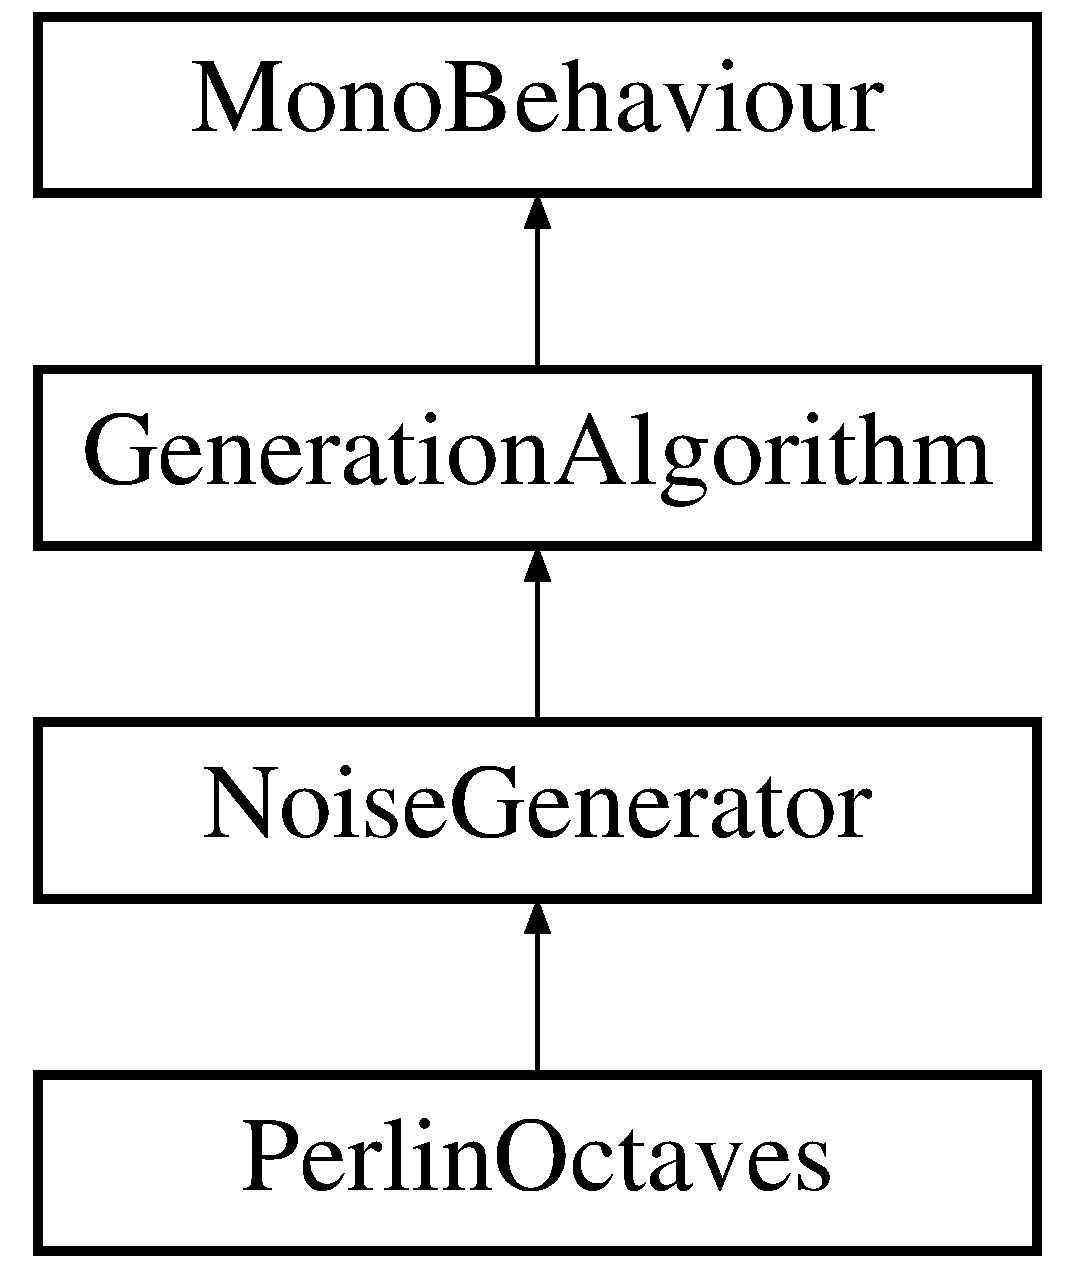
\includegraphics[height=4.000000cm]{class_perlin_octaves}
\end{center}
\end{figure}
\subsection*{Public Member Functions}
\begin{DoxyCompactItemize}
\item 
override float \mbox{[},\mbox{]} \mbox{\hyperlink{class_perlin_octaves_ac5deb001801dbfe9666df3dea023ce7a}{Generate\+Height\+Map}} (int map\+Width, int map\+Height)
\end{DoxyCompactItemize}
\subsection*{Static Public Member Functions}
\begin{DoxyCompactItemize}
\item 
static Vector2 \mbox{[}$\,$\mbox{]} \mbox{\hyperlink{class_perlin_octaves_a1a9290ee85b1250215cd042223cc7ed9}{Generate\+Offsets}} (int num\+Offsets, Vector2 additive)
\item 
static float \mbox{[},\mbox{]} \mbox{\hyperlink{class_perlin_octaves_acb953d3791014b27123139aee969f9bd}{Generate\+Noise\+Map}} (int map\+Width, int map\+Height, int seed, float \mbox{\hyperlink{class_noise_generator_a411009c00c7e62e99dccd0dd3b98c661}{scale}}, int octaves, float \mbox{\hyperlink{class_perlin_octaves_a0568ba2145fef1efb6bb137df4055a8a}{persistance}}, float \mbox{\hyperlink{class_perlin_octaves_a77574e7d920b80d15916798a4a7900d7}{lacunarity}}, Vector2 \mbox{\hyperlink{class_perlin_octaves_a86b7b4fa2c1f94e01a37748511ddb8ee}{offset}})
\end{DoxyCompactItemize}
\subsection*{Public Attributes}
\begin{DoxyCompactItemize}
\item 
int \mbox{\hyperlink{class_perlin_octaves_a611e17877eb36a3bdb546feae4d512cf}{num\+Octaves}} = 5
\item 
Vector2 \mbox{\hyperlink{class_perlin_octaves_a86b7b4fa2c1f94e01a37748511ddb8ee}{offset}} = new Vector2(51.\+11f, 0f)
\item 
float \mbox{\hyperlink{class_perlin_octaves_a0568ba2145fef1efb6bb137df4055a8a}{persistance}} = 0.\+5f
\item 
float \mbox{\hyperlink{class_perlin_octaves_a77574e7d920b80d15916798a4a7900d7}{lacunarity}} = 2f
\end{DoxyCompactItemize}
\subsection*{Additional Inherited Members}


\subsection{Member Function Documentation}
\mbox{\Hypertarget{class_perlin_octaves_ac5deb001801dbfe9666df3dea023ce7a}\label{class_perlin_octaves_ac5deb001801dbfe9666df3dea023ce7a}} 
\index{Perlin\+Octaves@{Perlin\+Octaves}!Generate\+Height\+Map@{Generate\+Height\+Map}}
\index{Generate\+Height\+Map@{Generate\+Height\+Map}!Perlin\+Octaves@{Perlin\+Octaves}}
\subsubsection{\texorpdfstring{Generate\+Height\+Map()}{GenerateHeightMap()}}
{\footnotesize\ttfamily override float \mbox{[},\mbox{]} Perlin\+Octaves.\+Generate\+Height\+Map (\begin{DoxyParamCaption}\item[{int}]{map\+Width,  }\item[{int}]{map\+Height }\end{DoxyParamCaption})\hspace{0.3cm}{\ttfamily [virtual]}}



Implements \mbox{\hyperlink{class_noise_generator_a1d3983a9ad33c2734f373e9f2d8f13d7}{Noise\+Generator}}.

\mbox{\Hypertarget{class_perlin_octaves_acb953d3791014b27123139aee969f9bd}\label{class_perlin_octaves_acb953d3791014b27123139aee969f9bd}} 
\index{Perlin\+Octaves@{Perlin\+Octaves}!Generate\+Noise\+Map@{Generate\+Noise\+Map}}
\index{Generate\+Noise\+Map@{Generate\+Noise\+Map}!Perlin\+Octaves@{Perlin\+Octaves}}
\subsubsection{\texorpdfstring{Generate\+Noise\+Map()}{GenerateNoiseMap()}}
{\footnotesize\ttfamily static float \mbox{[},\mbox{]} Perlin\+Octaves.\+Generate\+Noise\+Map (\begin{DoxyParamCaption}\item[{int}]{map\+Width,  }\item[{int}]{map\+Height,  }\item[{int}]{seed,  }\item[{float}]{scale,  }\item[{int}]{octaves,  }\item[{float}]{persistance,  }\item[{float}]{lacunarity,  }\item[{Vector2}]{offset }\end{DoxyParamCaption})\hspace{0.3cm}{\ttfamily [static]}}

\mbox{\Hypertarget{class_perlin_octaves_a1a9290ee85b1250215cd042223cc7ed9}\label{class_perlin_octaves_a1a9290ee85b1250215cd042223cc7ed9}} 
\index{Perlin\+Octaves@{Perlin\+Octaves}!Generate\+Offsets@{Generate\+Offsets}}
\index{Generate\+Offsets@{Generate\+Offsets}!Perlin\+Octaves@{Perlin\+Octaves}}
\subsubsection{\texorpdfstring{Generate\+Offsets()}{GenerateOffsets()}}
{\footnotesize\ttfamily static Vector2 \mbox{[}$\,$\mbox{]} Perlin\+Octaves.\+Generate\+Offsets (\begin{DoxyParamCaption}\item[{int}]{num\+Offsets,  }\item[{Vector2}]{additive }\end{DoxyParamCaption})\hspace{0.3cm}{\ttfamily [static]}}



\subsection{Member Data Documentation}
\mbox{\Hypertarget{class_perlin_octaves_a77574e7d920b80d15916798a4a7900d7}\label{class_perlin_octaves_a77574e7d920b80d15916798a4a7900d7}} 
\index{Perlin\+Octaves@{Perlin\+Octaves}!lacunarity@{lacunarity}}
\index{lacunarity@{lacunarity}!Perlin\+Octaves@{Perlin\+Octaves}}
\subsubsection{\texorpdfstring{lacunarity}{lacunarity}}
{\footnotesize\ttfamily float Perlin\+Octaves.\+lacunarity = 2f}

\mbox{\Hypertarget{class_perlin_octaves_a611e17877eb36a3bdb546feae4d512cf}\label{class_perlin_octaves_a611e17877eb36a3bdb546feae4d512cf}} 
\index{Perlin\+Octaves@{Perlin\+Octaves}!num\+Octaves@{num\+Octaves}}
\index{num\+Octaves@{num\+Octaves}!Perlin\+Octaves@{Perlin\+Octaves}}
\subsubsection{\texorpdfstring{num\+Octaves}{numOctaves}}
{\footnotesize\ttfamily int Perlin\+Octaves.\+num\+Octaves = 5}

\mbox{\Hypertarget{class_perlin_octaves_a86b7b4fa2c1f94e01a37748511ddb8ee}\label{class_perlin_octaves_a86b7b4fa2c1f94e01a37748511ddb8ee}} 
\index{Perlin\+Octaves@{Perlin\+Octaves}!offset@{offset}}
\index{offset@{offset}!Perlin\+Octaves@{Perlin\+Octaves}}
\subsubsection{\texorpdfstring{offset}{offset}}
{\footnotesize\ttfamily Vector2 Perlin\+Octaves.\+offset = new Vector2(51.\+11f, 0f)}

\mbox{\Hypertarget{class_perlin_octaves_a0568ba2145fef1efb6bb137df4055a8a}\label{class_perlin_octaves_a0568ba2145fef1efb6bb137df4055a8a}} 
\index{Perlin\+Octaves@{Perlin\+Octaves}!persistance@{persistance}}
\index{persistance@{persistance}!Perlin\+Octaves@{Perlin\+Octaves}}
\subsubsection{\texorpdfstring{persistance}{persistance}}
{\footnotesize\ttfamily float Perlin\+Octaves.\+persistance = 0.\+5f}



The documentation for this class was generated from the following file\+:\begin{DoxyCompactItemize}
\item 
/\+Users/sabienambrose/\+Documents/\+Coding/\+Unity\+Mechanical\+Turk/\+Mechanical\+Turk/\+Assets/\+Scripts/\+Generation/\mbox{\hyperlink{_perlin_octaves_8cs}{Perlin\+Octaves.\+cs}}\end{DoxyCompactItemize}

\hypertarget{class_point_generator}{}\section{Point\+Generator Class Reference}
\label{class_point_generator}\index{Point\+Generator@{Point\+Generator}}
Inheritance diagram for Point\+Generator\+:\begin{figure}[H]
\begin{center}
\leavevmode
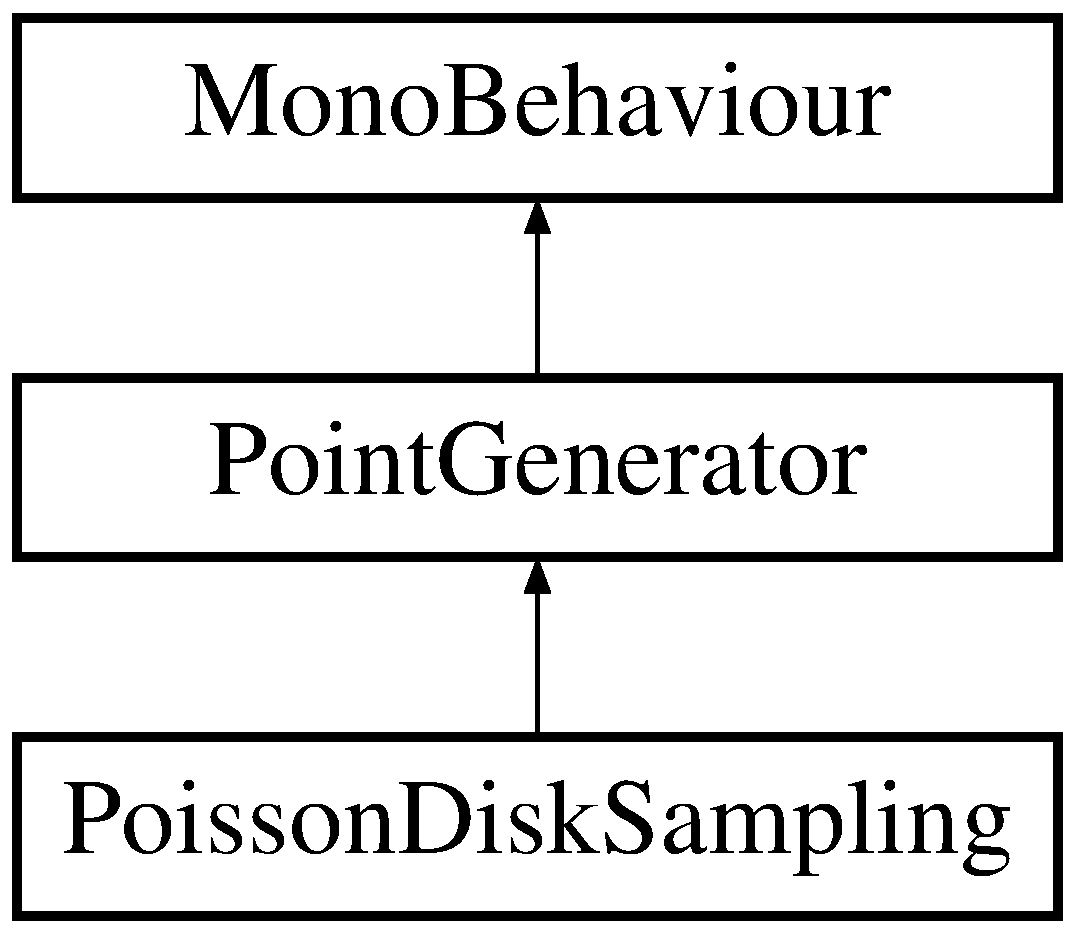
\includegraphics[height=3.000000cm]{class_point_generator}
\end{center}
\end{figure}
\subsection*{Public Member Functions}
\begin{DoxyCompactItemize}
\item 
virtual Vector2 \mbox{\hyperlink{class_point_generator_a58500ea3c2c04ee376b6f85e53c65509}{Rand\+Point}} ()
\item 
virtual Vector2 \mbox{\hyperlink{class_point_generator_a91e70f9d4939dfb00755b46937e6d26b}{Next\+Point}} ()
\item 
Vector2 \mbox{[}$\,$\mbox{]} \mbox{\hyperlink{class_point_generator_a94c7b1d2e704fedde36309423cc0c609}{Corners}} ()
\item 
abstract void \mbox{\hyperlink{class_point_generator_ae254f890c9a38d044d77f981e0dfeb68}{Init}} ()
\item 
abstract void \mbox{\hyperlink{class_point_generator_a46241ac6f86e8a9cd190bbecba41f6d1}{Init}} (Vector2\mbox{[}$\,$\mbox{]} source\+Points)
\item 
abstract void \mbox{\hyperlink{class_point_generator_aa952bfb78a0b3d97db614f9f8d062747}{Generate}} (out List$<$ Vector2 $>$ results)
\item 
abstract void \mbox{\hyperlink{class_point_generator_a9552a67546e0f4a0d96cd300c656c94e}{Generate}} (float width, float height, float min\+Dstance, int max\+Points\+Desired, out List$<$ Vector2 $>$ results)
\end{DoxyCompactItemize}
\subsection*{Public Attributes}
\begin{DoxyCompactItemize}
\item 
Polygon\+Collider2D \mbox{\hyperlink{class_point_generator_ade370757db1179941702a6eb1944d6ea}{bounds}}
\item 
List$<$ Vector2 $>$ \mbox{\hyperlink{class_point_generator_a8ab671e3c028583108b4e90425a49b6b}{sample\+Points}}
\end{DoxyCompactItemize}


\subsection{Member Function Documentation}
\mbox{\Hypertarget{class_point_generator_a94c7b1d2e704fedde36309423cc0c609}\label{class_point_generator_a94c7b1d2e704fedde36309423cc0c609}} 
\index{Point\+Generator@{Point\+Generator}!Corners@{Corners}}
\index{Corners@{Corners}!Point\+Generator@{Point\+Generator}}
\subsubsection{\texorpdfstring{Corners()}{Corners()}}
{\footnotesize\ttfamily Vector2 \mbox{[}$\,$\mbox{]} Point\+Generator.\+Corners (\begin{DoxyParamCaption}{ }\end{DoxyParamCaption})}

\mbox{\Hypertarget{class_point_generator_aa952bfb78a0b3d97db614f9f8d062747}\label{class_point_generator_aa952bfb78a0b3d97db614f9f8d062747}} 
\index{Point\+Generator@{Point\+Generator}!Generate@{Generate}}
\index{Generate@{Generate}!Point\+Generator@{Point\+Generator}}
\subsubsection{\texorpdfstring{Generate()}{Generate()}\hspace{0.1cm}{\footnotesize\ttfamily [1/2]}}
{\footnotesize\ttfamily abstract void Point\+Generator.\+Generate (\begin{DoxyParamCaption}\item[{out List$<$ Vector2 $>$}]{results }\end{DoxyParamCaption})\hspace{0.3cm}{\ttfamily [pure virtual]}}



Implemented in \mbox{\hyperlink{class_poisson_disk_sampling_a93700de987a5b4bf64da7cd0db070534}{Poisson\+Disk\+Sampling}}.

\mbox{\Hypertarget{class_point_generator_a9552a67546e0f4a0d96cd300c656c94e}\label{class_point_generator_a9552a67546e0f4a0d96cd300c656c94e}} 
\index{Point\+Generator@{Point\+Generator}!Generate@{Generate}}
\index{Generate@{Generate}!Point\+Generator@{Point\+Generator}}
\subsubsection{\texorpdfstring{Generate()}{Generate()}\hspace{0.1cm}{\footnotesize\ttfamily [2/2]}}
{\footnotesize\ttfamily abstract void Point\+Generator.\+Generate (\begin{DoxyParamCaption}\item[{float}]{width,  }\item[{float}]{height,  }\item[{float}]{min\+Dstance,  }\item[{int}]{max\+Points\+Desired,  }\item[{out List$<$ Vector2 $>$}]{results }\end{DoxyParamCaption})\hspace{0.3cm}{\ttfamily [pure virtual]}}



Implemented in \mbox{\hyperlink{class_poisson_disk_sampling_af2aeccc94efa7d224044f730fc432bcf}{Poisson\+Disk\+Sampling}}.

\mbox{\Hypertarget{class_point_generator_ae254f890c9a38d044d77f981e0dfeb68}\label{class_point_generator_ae254f890c9a38d044d77f981e0dfeb68}} 
\index{Point\+Generator@{Point\+Generator}!Init@{Init}}
\index{Init@{Init}!Point\+Generator@{Point\+Generator}}
\subsubsection{\texorpdfstring{Init()}{Init()}\hspace{0.1cm}{\footnotesize\ttfamily [1/2]}}
{\footnotesize\ttfamily abstract void Point\+Generator.\+Init (\begin{DoxyParamCaption}{ }\end{DoxyParamCaption})\hspace{0.3cm}{\ttfamily [pure virtual]}}



Implemented in \mbox{\hyperlink{class_poisson_disk_sampling_a1a571483a8940424916aa1266576161e}{Poisson\+Disk\+Sampling}}.

\mbox{\Hypertarget{class_point_generator_a46241ac6f86e8a9cd190bbecba41f6d1}\label{class_point_generator_a46241ac6f86e8a9cd190bbecba41f6d1}} 
\index{Point\+Generator@{Point\+Generator}!Init@{Init}}
\index{Init@{Init}!Point\+Generator@{Point\+Generator}}
\subsubsection{\texorpdfstring{Init()}{Init()}\hspace{0.1cm}{\footnotesize\ttfamily [2/2]}}
{\footnotesize\ttfamily abstract void Point\+Generator.\+Init (\begin{DoxyParamCaption}\item[{Vector2 \mbox{[}$\,$\mbox{]}}]{source\+Points }\end{DoxyParamCaption})\hspace{0.3cm}{\ttfamily [pure virtual]}}



Implemented in \mbox{\hyperlink{class_poisson_disk_sampling_abd6053768abe24749eee699ce914eceb}{Poisson\+Disk\+Sampling}}.

\mbox{\Hypertarget{class_point_generator_a91e70f9d4939dfb00755b46937e6d26b}\label{class_point_generator_a91e70f9d4939dfb00755b46937e6d26b}} 
\index{Point\+Generator@{Point\+Generator}!Next\+Point@{Next\+Point}}
\index{Next\+Point@{Next\+Point}!Point\+Generator@{Point\+Generator}}
\subsubsection{\texorpdfstring{Next\+Point()}{NextPoint()}}
{\footnotesize\ttfamily virtual Vector2 Point\+Generator.\+Next\+Point (\begin{DoxyParamCaption}{ }\end{DoxyParamCaption})\hspace{0.3cm}{\ttfamily [virtual]}}



Reimplemented in \mbox{\hyperlink{class_poisson_disk_sampling_a6e0e9060e58c98193329d0661a64a5ed}{Poisson\+Disk\+Sampling}}.

\mbox{\Hypertarget{class_point_generator_a58500ea3c2c04ee376b6f85e53c65509}\label{class_point_generator_a58500ea3c2c04ee376b6f85e53c65509}} 
\index{Point\+Generator@{Point\+Generator}!Rand\+Point@{Rand\+Point}}
\index{Rand\+Point@{Rand\+Point}!Point\+Generator@{Point\+Generator}}
\subsubsection{\texorpdfstring{Rand\+Point()}{RandPoint()}}
{\footnotesize\ttfamily virtual Vector2 Point\+Generator.\+Rand\+Point (\begin{DoxyParamCaption}{ }\end{DoxyParamCaption})\hspace{0.3cm}{\ttfamily [virtual]}}



\subsection{Member Data Documentation}
\mbox{\Hypertarget{class_point_generator_ade370757db1179941702a6eb1944d6ea}\label{class_point_generator_ade370757db1179941702a6eb1944d6ea}} 
\index{Point\+Generator@{Point\+Generator}!bounds@{bounds}}
\index{bounds@{bounds}!Point\+Generator@{Point\+Generator}}
\subsubsection{\texorpdfstring{bounds}{bounds}}
{\footnotesize\ttfamily Polygon\+Collider2D Point\+Generator.\+bounds}

\mbox{\Hypertarget{class_point_generator_a8ab671e3c028583108b4e90425a49b6b}\label{class_point_generator_a8ab671e3c028583108b4e90425a49b6b}} 
\index{Point\+Generator@{Point\+Generator}!sample\+Points@{sample\+Points}}
\index{sample\+Points@{sample\+Points}!Point\+Generator@{Point\+Generator}}
\subsubsection{\texorpdfstring{sample\+Points}{samplePoints}}
{\footnotesize\ttfamily List$<$Vector2$>$ Point\+Generator.\+sample\+Points}



The documentation for this class was generated from the following file\+:\begin{DoxyCompactItemize}
\item 
/\+Users/sabienambrose/\+Documents/\+Coding/\+Unity\+Mechanical\+Turk/\+Mechanical\+Turk/\+Assets/\+Scripts/\+Framework/\+Generation/\mbox{\hyperlink{_point_generator_8cs}{Point\+Generator.\+cs}}\end{DoxyCompactItemize}

\hypertarget{class_poisson_disk_sampling}{}\section{Poisson\+Disk\+Sampling Class Reference}
\label{class_poisson_disk_sampling}\index{Poisson\+Disk\+Sampling@{Poisson\+Disk\+Sampling}}
Inheritance diagram for Poisson\+Disk\+Sampling\+:\begin{figure}[H]
\begin{center}
\leavevmode
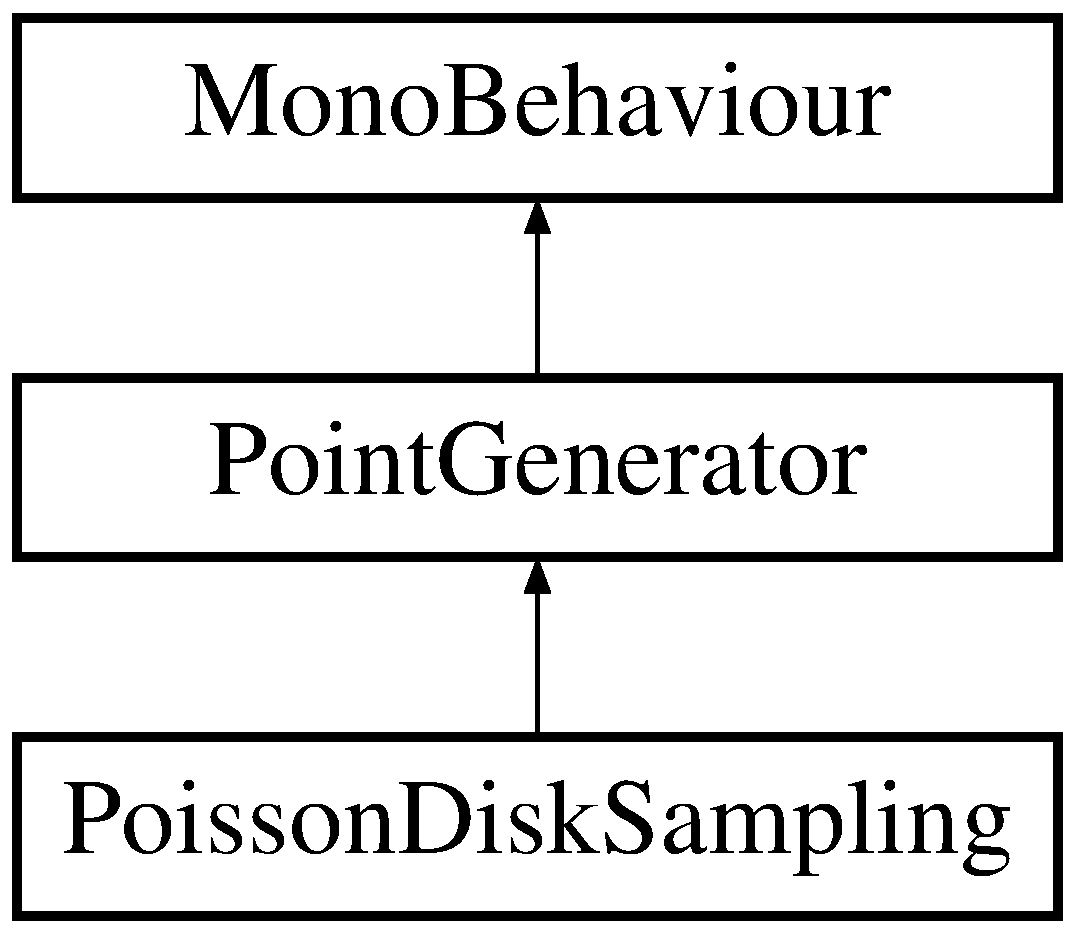
\includegraphics[height=3.000000cm]{class_poisson_disk_sampling}
\end{center}
\end{figure}
\subsection*{Public Member Functions}
\begin{DoxyCompactItemize}
\item 
override void \mbox{\hyperlink{class_poisson_disk_sampling_a1a571483a8940424916aa1266576161e}{Init}} ()
\item 
override void \mbox{\hyperlink{class_poisson_disk_sampling_abd6053768abe24749eee699ce914eceb}{Init}} (Vector2\mbox{[}$\,$\mbox{]} source\+Points)
\item 
void \mbox{\hyperlink{class_poisson_disk_sampling_a5d3b4212b8f786be4e849b93ca096ab6}{Next\+Source\+Point}} ()
\item 
Vector2 \mbox{\hyperlink{class_poisson_disk_sampling_a4d173da254062579395c756861467e93}{Make\+Random\+Point}} ()
\item 
override Vector2 \mbox{\hyperlink{class_poisson_disk_sampling_a6e0e9060e58c98193329d0661a64a5ed}{Next\+Point}} ()
\item 
void \mbox{\hyperlink{class_poisson_disk_sampling_a96daccb88a2edb1f835d3ed8e19ace2e}{Generate\+Poisson}} ()
\item 
void \mbox{\hyperlink{class_poisson_disk_sampling_acfa775a97fe1210f2b28188464f8092b}{Add\+Point}} (Vector2 In\+Point)
\item 
Vector2 \mbox{\hyperlink{class_poisson_disk_sampling_aadc97855167d6531a56c9099101877d0}{Generate\+Random\+Point\+Around}} (Vector2 point, float min\+Dist)
\item 
\mbox{\hyperlink{struct_int_point}{Int\+Point}} \mbox{\hyperlink{class_poisson_disk_sampling_a3489e3f81cc5c5fa5087e8edb7042659}{Point\+To\+Grid\+Coord}} (Vector2 point)
\item 
override void \mbox{\hyperlink{class_poisson_disk_sampling_a93700de987a5b4bf64da7cd0db070534}{Generate}} (out List$<$ Vector2 $>$ results)
\item 
override void \mbox{\hyperlink{class_poisson_disk_sampling_af2aeccc94efa7d224044f730fc432bcf}{Generate}} (float \mbox{\hyperlink{class_poisson_disk_sampling_a0b32f3e1950036797fb17575da924b8e}{width}}, float \mbox{\hyperlink{class_poisson_disk_sampling_aa75a106477c40f9d1200f3ae71dd544f}{height}}, float min\+Dstance, int max\+Points\+Desired, out List$<$ Vector2 $>$ results)
\end{DoxyCompactItemize}
\subsection*{Public Attributes}
\begin{DoxyCompactItemize}
\item 
float \mbox{\hyperlink{class_poisson_disk_sampling_a0b32f3e1950036797fb17575da924b8e}{width}} = 100
\item 
float \mbox{\hyperlink{class_poisson_disk_sampling_aa75a106477c40f9d1200f3ae71dd544f}{height}} = 100
\item 
float \mbox{\hyperlink{class_poisson_disk_sampling_a5e7060326d72754ea94c25df1d5afbaf}{min\+Distance}} = 5
\item 
int \mbox{\hyperlink{class_poisson_disk_sampling_a2ff267a5d6d3a2f30c613ce52ae48bf8}{new\+Points\+Count}} = 30
\item 
int \mbox{\hyperlink{class_poisson_disk_sampling_a1c7892b887f1405caedef95ab667735e}{max\+Total\+Points}} = 1000
\item 
\mbox{\hyperlink{struct_grid2_d}{Grid2D}} \mbox{\hyperlink{class_poisson_disk_sampling_a7cc5fef43fe82e98bb385d76f4df3727}{grid}}
\end{DoxyCompactItemize}


\subsection{Member Function Documentation}
\mbox{\Hypertarget{class_poisson_disk_sampling_acfa775a97fe1210f2b28188464f8092b}\label{class_poisson_disk_sampling_acfa775a97fe1210f2b28188464f8092b}} 
\index{Poisson\+Disk\+Sampling@{Poisson\+Disk\+Sampling}!Add\+Point@{Add\+Point}}
\index{Add\+Point@{Add\+Point}!Poisson\+Disk\+Sampling@{Poisson\+Disk\+Sampling}}
\subsubsection{\texorpdfstring{Add\+Point()}{AddPoint()}}
{\footnotesize\ttfamily void Poisson\+Disk\+Sampling.\+Add\+Point (\begin{DoxyParamCaption}\item[{Vector2}]{In\+Point }\end{DoxyParamCaption})}

\mbox{\Hypertarget{class_poisson_disk_sampling_a93700de987a5b4bf64da7cd0db070534}\label{class_poisson_disk_sampling_a93700de987a5b4bf64da7cd0db070534}} 
\index{Poisson\+Disk\+Sampling@{Poisson\+Disk\+Sampling}!Generate@{Generate}}
\index{Generate@{Generate}!Poisson\+Disk\+Sampling@{Poisson\+Disk\+Sampling}}
\subsubsection{\texorpdfstring{Generate()}{Generate()}\hspace{0.1cm}{\footnotesize\ttfamily [1/2]}}
{\footnotesize\ttfamily override void Poisson\+Disk\+Sampling.\+Generate (\begin{DoxyParamCaption}\item[{out List$<$ Vector2 $>$}]{results }\end{DoxyParamCaption})\hspace{0.3cm}{\ttfamily [virtual]}}



Implements \mbox{\hyperlink{class_point_generator_aa952bfb78a0b3d97db614f9f8d062747}{Point\+Generator}}.

\mbox{\Hypertarget{class_poisson_disk_sampling_af2aeccc94efa7d224044f730fc432bcf}\label{class_poisson_disk_sampling_af2aeccc94efa7d224044f730fc432bcf}} 
\index{Poisson\+Disk\+Sampling@{Poisson\+Disk\+Sampling}!Generate@{Generate}}
\index{Generate@{Generate}!Poisson\+Disk\+Sampling@{Poisson\+Disk\+Sampling}}
\subsubsection{\texorpdfstring{Generate()}{Generate()}\hspace{0.1cm}{\footnotesize\ttfamily [2/2]}}
{\footnotesize\ttfamily override void Poisson\+Disk\+Sampling.\+Generate (\begin{DoxyParamCaption}\item[{float}]{width,  }\item[{float}]{height,  }\item[{float}]{min\+Dstance,  }\item[{int}]{max\+Points\+Desired,  }\item[{out List$<$ Vector2 $>$}]{results }\end{DoxyParamCaption})\hspace{0.3cm}{\ttfamily [virtual]}}



Implements \mbox{\hyperlink{class_point_generator_a9552a67546e0f4a0d96cd300c656c94e}{Point\+Generator}}.

\mbox{\Hypertarget{class_poisson_disk_sampling_a96daccb88a2edb1f835d3ed8e19ace2e}\label{class_poisson_disk_sampling_a96daccb88a2edb1f835d3ed8e19ace2e}} 
\index{Poisson\+Disk\+Sampling@{Poisson\+Disk\+Sampling}!Generate\+Poisson@{Generate\+Poisson}}
\index{Generate\+Poisson@{Generate\+Poisson}!Poisson\+Disk\+Sampling@{Poisson\+Disk\+Sampling}}
\subsubsection{\texorpdfstring{Generate\+Poisson()}{GeneratePoisson()}}
{\footnotesize\ttfamily void Poisson\+Disk\+Sampling.\+Generate\+Poisson (\begin{DoxyParamCaption}{ }\end{DoxyParamCaption})}

\mbox{\Hypertarget{class_poisson_disk_sampling_aadc97855167d6531a56c9099101877d0}\label{class_poisson_disk_sampling_aadc97855167d6531a56c9099101877d0}} 
\index{Poisson\+Disk\+Sampling@{Poisson\+Disk\+Sampling}!Generate\+Random\+Point\+Around@{Generate\+Random\+Point\+Around}}
\index{Generate\+Random\+Point\+Around@{Generate\+Random\+Point\+Around}!Poisson\+Disk\+Sampling@{Poisson\+Disk\+Sampling}}
\subsubsection{\texorpdfstring{Generate\+Random\+Point\+Around()}{GenerateRandomPointAround()}}
{\footnotesize\ttfamily Vector2 Poisson\+Disk\+Sampling.\+Generate\+Random\+Point\+Around (\begin{DoxyParamCaption}\item[{Vector2}]{point,  }\item[{float}]{min\+Dist }\end{DoxyParamCaption})}

\mbox{\Hypertarget{class_poisson_disk_sampling_a1a571483a8940424916aa1266576161e}\label{class_poisson_disk_sampling_a1a571483a8940424916aa1266576161e}} 
\index{Poisson\+Disk\+Sampling@{Poisson\+Disk\+Sampling}!Init@{Init}}
\index{Init@{Init}!Poisson\+Disk\+Sampling@{Poisson\+Disk\+Sampling}}
\subsubsection{\texorpdfstring{Init()}{Init()}\hspace{0.1cm}{\footnotesize\ttfamily [1/2]}}
{\footnotesize\ttfamily override void Poisson\+Disk\+Sampling.\+Init (\begin{DoxyParamCaption}{ }\end{DoxyParamCaption})\hspace{0.3cm}{\ttfamily [virtual]}}



Implements \mbox{\hyperlink{class_point_generator_ae254f890c9a38d044d77f981e0dfeb68}{Point\+Generator}}.

\mbox{\Hypertarget{class_poisson_disk_sampling_abd6053768abe24749eee699ce914eceb}\label{class_poisson_disk_sampling_abd6053768abe24749eee699ce914eceb}} 
\index{Poisson\+Disk\+Sampling@{Poisson\+Disk\+Sampling}!Init@{Init}}
\index{Init@{Init}!Poisson\+Disk\+Sampling@{Poisson\+Disk\+Sampling}}
\subsubsection{\texorpdfstring{Init()}{Init()}\hspace{0.1cm}{\footnotesize\ttfamily [2/2]}}
{\footnotesize\ttfamily override void Poisson\+Disk\+Sampling.\+Init (\begin{DoxyParamCaption}\item[{Vector2 \mbox{[}$\,$\mbox{]}}]{source\+Points }\end{DoxyParamCaption})\hspace{0.3cm}{\ttfamily [virtual]}}



Implements \mbox{\hyperlink{class_point_generator_a46241ac6f86e8a9cd190bbecba41f6d1}{Point\+Generator}}.

\mbox{\Hypertarget{class_poisson_disk_sampling_a4d173da254062579395c756861467e93}\label{class_poisson_disk_sampling_a4d173da254062579395c756861467e93}} 
\index{Poisson\+Disk\+Sampling@{Poisson\+Disk\+Sampling}!Make\+Random\+Point@{Make\+Random\+Point}}
\index{Make\+Random\+Point@{Make\+Random\+Point}!Poisson\+Disk\+Sampling@{Poisson\+Disk\+Sampling}}
\subsubsection{\texorpdfstring{Make\+Random\+Point()}{MakeRandomPoint()}}
{\footnotesize\ttfamily Vector2 Poisson\+Disk\+Sampling.\+Make\+Random\+Point (\begin{DoxyParamCaption}{ }\end{DoxyParamCaption})}

\mbox{\Hypertarget{class_poisson_disk_sampling_a6e0e9060e58c98193329d0661a64a5ed}\label{class_poisson_disk_sampling_a6e0e9060e58c98193329d0661a64a5ed}} 
\index{Poisson\+Disk\+Sampling@{Poisson\+Disk\+Sampling}!Next\+Point@{Next\+Point}}
\index{Next\+Point@{Next\+Point}!Poisson\+Disk\+Sampling@{Poisson\+Disk\+Sampling}}
\subsubsection{\texorpdfstring{Next\+Point()}{NextPoint()}}
{\footnotesize\ttfamily override Vector2 Poisson\+Disk\+Sampling.\+Next\+Point (\begin{DoxyParamCaption}{ }\end{DoxyParamCaption})\hspace{0.3cm}{\ttfamily [virtual]}}



Reimplemented from \mbox{\hyperlink{class_point_generator_a91e70f9d4939dfb00755b46937e6d26b}{Point\+Generator}}.

\mbox{\Hypertarget{class_poisson_disk_sampling_a5d3b4212b8f786be4e849b93ca096ab6}\label{class_poisson_disk_sampling_a5d3b4212b8f786be4e849b93ca096ab6}} 
\index{Poisson\+Disk\+Sampling@{Poisson\+Disk\+Sampling}!Next\+Source\+Point@{Next\+Source\+Point}}
\index{Next\+Source\+Point@{Next\+Source\+Point}!Poisson\+Disk\+Sampling@{Poisson\+Disk\+Sampling}}
\subsubsection{\texorpdfstring{Next\+Source\+Point()}{NextSourcePoint()}}
{\footnotesize\ttfamily void Poisson\+Disk\+Sampling.\+Next\+Source\+Point (\begin{DoxyParamCaption}{ }\end{DoxyParamCaption})}

\mbox{\Hypertarget{class_poisson_disk_sampling_a3489e3f81cc5c5fa5087e8edb7042659}\label{class_poisson_disk_sampling_a3489e3f81cc5c5fa5087e8edb7042659}} 
\index{Poisson\+Disk\+Sampling@{Poisson\+Disk\+Sampling}!Point\+To\+Grid\+Coord@{Point\+To\+Grid\+Coord}}
\index{Point\+To\+Grid\+Coord@{Point\+To\+Grid\+Coord}!Poisson\+Disk\+Sampling@{Poisson\+Disk\+Sampling}}
\subsubsection{\texorpdfstring{Point\+To\+Grid\+Coord()}{PointToGridCoord()}}
{\footnotesize\ttfamily \mbox{\hyperlink{struct_int_point}{Int\+Point}} Poisson\+Disk\+Sampling.\+Point\+To\+Grid\+Coord (\begin{DoxyParamCaption}\item[{Vector2}]{point }\end{DoxyParamCaption})}



\subsection{Member Data Documentation}
\mbox{\Hypertarget{class_poisson_disk_sampling_a7cc5fef43fe82e98bb385d76f4df3727}\label{class_poisson_disk_sampling_a7cc5fef43fe82e98bb385d76f4df3727}} 
\index{Poisson\+Disk\+Sampling@{Poisson\+Disk\+Sampling}!grid@{grid}}
\index{grid@{grid}!Poisson\+Disk\+Sampling@{Poisson\+Disk\+Sampling}}
\subsubsection{\texorpdfstring{grid}{grid}}
{\footnotesize\ttfamily \mbox{\hyperlink{struct_grid2_d}{Grid2D}} Poisson\+Disk\+Sampling.\+grid}

\mbox{\Hypertarget{class_poisson_disk_sampling_aa75a106477c40f9d1200f3ae71dd544f}\label{class_poisson_disk_sampling_aa75a106477c40f9d1200f3ae71dd544f}} 
\index{Poisson\+Disk\+Sampling@{Poisson\+Disk\+Sampling}!height@{height}}
\index{height@{height}!Poisson\+Disk\+Sampling@{Poisson\+Disk\+Sampling}}
\subsubsection{\texorpdfstring{height}{height}}
{\footnotesize\ttfamily float Poisson\+Disk\+Sampling.\+height = 100}

\mbox{\Hypertarget{class_poisson_disk_sampling_a1c7892b887f1405caedef95ab667735e}\label{class_poisson_disk_sampling_a1c7892b887f1405caedef95ab667735e}} 
\index{Poisson\+Disk\+Sampling@{Poisson\+Disk\+Sampling}!max\+Total\+Points@{max\+Total\+Points}}
\index{max\+Total\+Points@{max\+Total\+Points}!Poisson\+Disk\+Sampling@{Poisson\+Disk\+Sampling}}
\subsubsection{\texorpdfstring{max\+Total\+Points}{maxTotalPoints}}
{\footnotesize\ttfamily int Poisson\+Disk\+Sampling.\+max\+Total\+Points = 1000}

\mbox{\Hypertarget{class_poisson_disk_sampling_a5e7060326d72754ea94c25df1d5afbaf}\label{class_poisson_disk_sampling_a5e7060326d72754ea94c25df1d5afbaf}} 
\index{Poisson\+Disk\+Sampling@{Poisson\+Disk\+Sampling}!min\+Distance@{min\+Distance}}
\index{min\+Distance@{min\+Distance}!Poisson\+Disk\+Sampling@{Poisson\+Disk\+Sampling}}
\subsubsection{\texorpdfstring{min\+Distance}{minDistance}}
{\footnotesize\ttfamily float Poisson\+Disk\+Sampling.\+min\+Distance = 5}

\mbox{\Hypertarget{class_poisson_disk_sampling_a2ff267a5d6d3a2f30c613ce52ae48bf8}\label{class_poisson_disk_sampling_a2ff267a5d6d3a2f30c613ce52ae48bf8}} 
\index{Poisson\+Disk\+Sampling@{Poisson\+Disk\+Sampling}!new\+Points\+Count@{new\+Points\+Count}}
\index{new\+Points\+Count@{new\+Points\+Count}!Poisson\+Disk\+Sampling@{Poisson\+Disk\+Sampling}}
\subsubsection{\texorpdfstring{new\+Points\+Count}{newPointsCount}}
{\footnotesize\ttfamily int Poisson\+Disk\+Sampling.\+new\+Points\+Count = 30}

\mbox{\Hypertarget{class_poisson_disk_sampling_a0b32f3e1950036797fb17575da924b8e}\label{class_poisson_disk_sampling_a0b32f3e1950036797fb17575da924b8e}} 
\index{Poisson\+Disk\+Sampling@{Poisson\+Disk\+Sampling}!width@{width}}
\index{width@{width}!Poisson\+Disk\+Sampling@{Poisson\+Disk\+Sampling}}
\subsubsection{\texorpdfstring{width}{width}}
{\footnotesize\ttfamily float Poisson\+Disk\+Sampling.\+width = 100}



The documentation for this class was generated from the following file\+:\begin{DoxyCompactItemize}
\item 
/\+Users/sabienambrose/\+Documents/\+Coding/\+Unity\+Mechanical\+Turk/\+Mechanical\+Turk/\+Assets/\+Scripts/\+Generation/\mbox{\hyperlink{_poisson_disk_sampling_8cs}{Poisson\+Disk\+Sampling.\+cs}}\end{DoxyCompactItemize}

\hypertarget{class_poly_grid}{}\section{Poly\+Grid Class Reference}
\label{class_poly_grid}\index{Poly\+Grid@{Poly\+Grid}}
Inheritance diagram for Poly\+Grid\+:\begin{figure}[H]
\begin{center}
\leavevmode
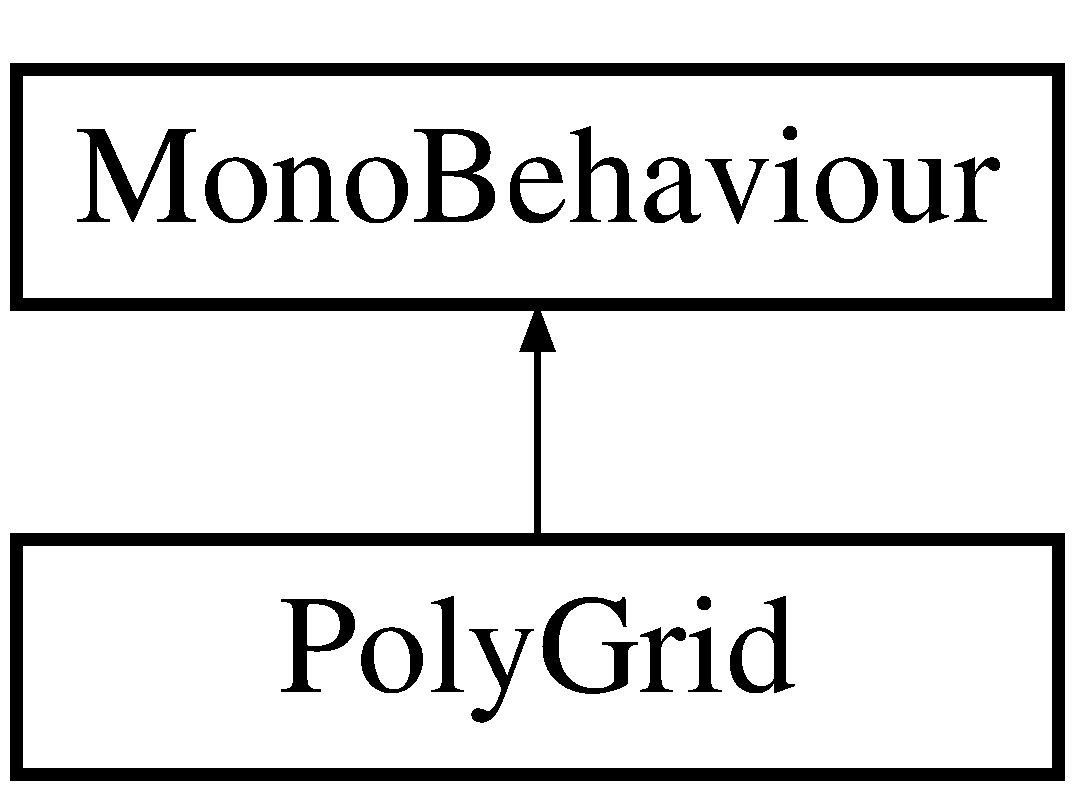
\includegraphics[height=2.000000cm]{class_poly_grid}
\end{center}
\end{figure}
\subsection*{Public Member Functions}
\begin{DoxyCompactItemize}
\item 
int \mbox{\hyperlink{class_poly_grid_abdcb8932a005a5cbd833430662727faf}{Num\+Faces}} ()
\item 
void \mbox{\hyperlink{class_poly_grid_a0fc1f57b2840e01acfc2d7dbe49d2fd1}{Add\+Face}} (\mbox{\hyperlink{class_grid_face}{Grid\+Face}} new\+Face)
\item 
void \mbox{\hyperlink{class_poly_grid_a486c7e7a5829e4bb9966c064db28113d}{Add\+Vertex}} (\mbox{\hyperlink{class_node}{Node}} new\+Vertex)
\item 
List$<$ \mbox{\hyperlink{class_node}{Node}} $>$ \mbox{\hyperlink{class_poly_grid_a35e759e3c28917350c1158e80a664a79}{Get\+Vertices}} ()
\item 
List$<$ \mbox{\hyperlink{class_grid_face}{Grid\+Face}} $>$ \mbox{\hyperlink{class_poly_grid_a4fd6191d005e389d329fc5f855732015}{Get\+Faces}} ()
\item 
void \mbox{\hyperlink{class_poly_grid_a9a19971fbde8f1aaa806d54771857d8b}{Flip\+Axes}} ()
\item 
void \mbox{\hyperlink{class_poly_grid_a1c99b63c71be2e28b2f1b1ccdbdf1c26}{On\+Draw\+Gizmos}} ()
\item 
void \mbox{\hyperlink{class_poly_grid_ae3c6db975b79d96ebb9ec0c16cfda518}{Draw\+Vertices}} ()
\item 
void \mbox{\hyperlink{class_poly_grid_a322dbff12283b94455ad415f554675c6}{Draw\+Faces}} ()
\end{DoxyCompactItemize}
\subsection*{Public Attributes}
\begin{DoxyCompactItemize}
\item 
Vector2 \mbox{\hyperlink{class_poly_grid_aeebd9e2f028fa1d79b48a61cf65a6829}{Dimensions}}
\item 
Vector2\+Int \mbox{\hyperlink{class_poly_grid_aa3d72d505c3c008a5bd52a448d932840}{Faces\+Per\+Side}}
\end{DoxyCompactItemize}
\subsection*{Protected Attributes}
\begin{DoxyCompactItemize}
\item 
List$<$ \mbox{\hyperlink{class_grid_face}{Grid\+Face}} $>$ \mbox{\hyperlink{class_poly_grid_ad1f5acf9cfbd3a2ad7add30d87eb0416}{faces}} = new List$<$\mbox{\hyperlink{class_grid_face}{Grid\+Face}}$>$()
\item 
List$<$ \mbox{\hyperlink{class_node}{Node}} $>$ \mbox{\hyperlink{class_poly_grid_a40f18bd5bd749337828beb314e43a36e}{vertices}} = new List$<$\mbox{\hyperlink{class_node}{Node}}$>$()
\end{DoxyCompactItemize}


\subsection{Member Function Documentation}
\mbox{\Hypertarget{class_poly_grid_a0fc1f57b2840e01acfc2d7dbe49d2fd1}\label{class_poly_grid_a0fc1f57b2840e01acfc2d7dbe49d2fd1}} 
\index{Poly\+Grid@{Poly\+Grid}!Add\+Face@{Add\+Face}}
\index{Add\+Face@{Add\+Face}!Poly\+Grid@{Poly\+Grid}}
\subsubsection{\texorpdfstring{Add\+Face()}{AddFace()}}
{\footnotesize\ttfamily void Poly\+Grid.\+Add\+Face (\begin{DoxyParamCaption}\item[{\mbox{\hyperlink{class_grid_face}{Grid\+Face}}}]{new\+Face }\end{DoxyParamCaption})}

\mbox{\Hypertarget{class_poly_grid_a486c7e7a5829e4bb9966c064db28113d}\label{class_poly_grid_a486c7e7a5829e4bb9966c064db28113d}} 
\index{Poly\+Grid@{Poly\+Grid}!Add\+Vertex@{Add\+Vertex}}
\index{Add\+Vertex@{Add\+Vertex}!Poly\+Grid@{Poly\+Grid}}
\subsubsection{\texorpdfstring{Add\+Vertex()}{AddVertex()}}
{\footnotesize\ttfamily void Poly\+Grid.\+Add\+Vertex (\begin{DoxyParamCaption}\item[{\mbox{\hyperlink{class_node}{Node}}}]{new\+Vertex }\end{DoxyParamCaption})}

\mbox{\Hypertarget{class_poly_grid_a322dbff12283b94455ad415f554675c6}\label{class_poly_grid_a322dbff12283b94455ad415f554675c6}} 
\index{Poly\+Grid@{Poly\+Grid}!Draw\+Faces@{Draw\+Faces}}
\index{Draw\+Faces@{Draw\+Faces}!Poly\+Grid@{Poly\+Grid}}
\subsubsection{\texorpdfstring{Draw\+Faces()}{DrawFaces()}}
{\footnotesize\ttfamily void Poly\+Grid.\+Draw\+Faces (\begin{DoxyParamCaption}{ }\end{DoxyParamCaption})}

\mbox{\Hypertarget{class_poly_grid_ae3c6db975b79d96ebb9ec0c16cfda518}\label{class_poly_grid_ae3c6db975b79d96ebb9ec0c16cfda518}} 
\index{Poly\+Grid@{Poly\+Grid}!Draw\+Vertices@{Draw\+Vertices}}
\index{Draw\+Vertices@{Draw\+Vertices}!Poly\+Grid@{Poly\+Grid}}
\subsubsection{\texorpdfstring{Draw\+Vertices()}{DrawVertices()}}
{\footnotesize\ttfamily void Poly\+Grid.\+Draw\+Vertices (\begin{DoxyParamCaption}{ }\end{DoxyParamCaption})}

\mbox{\Hypertarget{class_poly_grid_a9a19971fbde8f1aaa806d54771857d8b}\label{class_poly_grid_a9a19971fbde8f1aaa806d54771857d8b}} 
\index{Poly\+Grid@{Poly\+Grid}!Flip\+Axes@{Flip\+Axes}}
\index{Flip\+Axes@{Flip\+Axes}!Poly\+Grid@{Poly\+Grid}}
\subsubsection{\texorpdfstring{Flip\+Axes()}{FlipAxes()}}
{\footnotesize\ttfamily void Poly\+Grid.\+Flip\+Axes (\begin{DoxyParamCaption}{ }\end{DoxyParamCaption})}

\mbox{\Hypertarget{class_poly_grid_a4fd6191d005e389d329fc5f855732015}\label{class_poly_grid_a4fd6191d005e389d329fc5f855732015}} 
\index{Poly\+Grid@{Poly\+Grid}!Get\+Faces@{Get\+Faces}}
\index{Get\+Faces@{Get\+Faces}!Poly\+Grid@{Poly\+Grid}}
\subsubsection{\texorpdfstring{Get\+Faces()}{GetFaces()}}
{\footnotesize\ttfamily List$<$\mbox{\hyperlink{class_grid_face}{Grid\+Face}}$>$ Poly\+Grid.\+Get\+Faces (\begin{DoxyParamCaption}{ }\end{DoxyParamCaption})}

\mbox{\Hypertarget{class_poly_grid_a35e759e3c28917350c1158e80a664a79}\label{class_poly_grid_a35e759e3c28917350c1158e80a664a79}} 
\index{Poly\+Grid@{Poly\+Grid}!Get\+Vertices@{Get\+Vertices}}
\index{Get\+Vertices@{Get\+Vertices}!Poly\+Grid@{Poly\+Grid}}
\subsubsection{\texorpdfstring{Get\+Vertices()}{GetVertices()}}
{\footnotesize\ttfamily List$<$\mbox{\hyperlink{class_node}{Node}}$>$ Poly\+Grid.\+Get\+Vertices (\begin{DoxyParamCaption}{ }\end{DoxyParamCaption})}

\mbox{\Hypertarget{class_poly_grid_abdcb8932a005a5cbd833430662727faf}\label{class_poly_grid_abdcb8932a005a5cbd833430662727faf}} 
\index{Poly\+Grid@{Poly\+Grid}!Num\+Faces@{Num\+Faces}}
\index{Num\+Faces@{Num\+Faces}!Poly\+Grid@{Poly\+Grid}}
\subsubsection{\texorpdfstring{Num\+Faces()}{NumFaces()}}
{\footnotesize\ttfamily int Poly\+Grid.\+Num\+Faces (\begin{DoxyParamCaption}{ }\end{DoxyParamCaption})}

\mbox{\Hypertarget{class_poly_grid_a1c99b63c71be2e28b2f1b1ccdbdf1c26}\label{class_poly_grid_a1c99b63c71be2e28b2f1b1ccdbdf1c26}} 
\index{Poly\+Grid@{Poly\+Grid}!On\+Draw\+Gizmos@{On\+Draw\+Gizmos}}
\index{On\+Draw\+Gizmos@{On\+Draw\+Gizmos}!Poly\+Grid@{Poly\+Grid}}
\subsubsection{\texorpdfstring{On\+Draw\+Gizmos()}{OnDrawGizmos()}}
{\footnotesize\ttfamily void Poly\+Grid.\+On\+Draw\+Gizmos (\begin{DoxyParamCaption}{ }\end{DoxyParamCaption})}



\subsection{Member Data Documentation}
\mbox{\Hypertarget{class_poly_grid_aeebd9e2f028fa1d79b48a61cf65a6829}\label{class_poly_grid_aeebd9e2f028fa1d79b48a61cf65a6829}} 
\index{Poly\+Grid@{Poly\+Grid}!Dimensions@{Dimensions}}
\index{Dimensions@{Dimensions}!Poly\+Grid@{Poly\+Grid}}
\subsubsection{\texorpdfstring{Dimensions}{Dimensions}}
{\footnotesize\ttfamily Vector2 Poly\+Grid.\+Dimensions}

\mbox{\Hypertarget{class_poly_grid_ad1f5acf9cfbd3a2ad7add30d87eb0416}\label{class_poly_grid_ad1f5acf9cfbd3a2ad7add30d87eb0416}} 
\index{Poly\+Grid@{Poly\+Grid}!faces@{faces}}
\index{faces@{faces}!Poly\+Grid@{Poly\+Grid}}
\subsubsection{\texorpdfstring{faces}{faces}}
{\footnotesize\ttfamily List$<$\mbox{\hyperlink{class_grid_face}{Grid\+Face}}$>$ Poly\+Grid.\+faces = new List$<$\mbox{\hyperlink{class_grid_face}{Grid\+Face}}$>$()\hspace{0.3cm}{\ttfamily [protected]}}

\mbox{\Hypertarget{class_poly_grid_aa3d72d505c3c008a5bd52a448d932840}\label{class_poly_grid_aa3d72d505c3c008a5bd52a448d932840}} 
\index{Poly\+Grid@{Poly\+Grid}!Faces\+Per\+Side@{Faces\+Per\+Side}}
\index{Faces\+Per\+Side@{Faces\+Per\+Side}!Poly\+Grid@{Poly\+Grid}}
\subsubsection{\texorpdfstring{Faces\+Per\+Side}{FacesPerSide}}
{\footnotesize\ttfamily Vector2\+Int Poly\+Grid.\+Faces\+Per\+Side}

\mbox{\Hypertarget{class_poly_grid_a40f18bd5bd749337828beb314e43a36e}\label{class_poly_grid_a40f18bd5bd749337828beb314e43a36e}} 
\index{Poly\+Grid@{Poly\+Grid}!vertices@{vertices}}
\index{vertices@{vertices}!Poly\+Grid@{Poly\+Grid}}
\subsubsection{\texorpdfstring{vertices}{vertices}}
{\footnotesize\ttfamily List$<$\mbox{\hyperlink{class_node}{Node}}$>$ Poly\+Grid.\+vertices = new List$<$\mbox{\hyperlink{class_node}{Node}}$>$()\hspace{0.3cm}{\ttfamily [protected]}}



The documentation for this class was generated from the following file\+:\begin{DoxyCompactItemize}
\item 
/\+Users/sabienambrose/\+Documents/\+Coding/\+Unity\+Mechanical\+Turk/\+Mechanical\+Turk/\+Assets/\+Scripts/\+Util/\+Containers/\+Graphs/\+Grids/\mbox{\hyperlink{_poly_grid_8cs}{Poly\+Grid.\+cs}}\end{DoxyCompactItemize}

\hypertarget{class_random_queue}{}\section{Random\+Queue$<$ T $>$ Class Template Reference}
\label{class_random_queue}\index{Random\+Queue$<$ T $>$@{Random\+Queue$<$ T $>$}}
\subsection*{Public Member Functions}
\begin{DoxyCompactItemize}
\item 
void \mbox{\hyperlink{class_random_queue_a9b04768a955285d6df22824f12874958}{Push}} (T item)
\item 
T \mbox{\hyperlink{class_random_queue_a15fed32fe3e55df6f1fe883e019525f1}{Pop}} ()
\item 
int \mbox{\hyperlink{class_random_queue_a711ffc77868ff152cb4f407b1f0cb8f8}{Count}} ()
\item 
bool \mbox{\hyperlink{class_random_queue_af19660c14e19e166a4632a37cba1a8c1}{Empty}} ()
\end{DoxyCompactItemize}
\subsection*{Protected Attributes}
\begin{DoxyCompactItemize}
\item 
List$<$ T $>$ \mbox{\hyperlink{class_random_queue_a33495067868e22aa274248df60013b11}{contents}} = new List$<$T$>$()
\end{DoxyCompactItemize}


\subsection{Member Function Documentation}
\mbox{\Hypertarget{class_random_queue_a711ffc77868ff152cb4f407b1f0cb8f8}\label{class_random_queue_a711ffc77868ff152cb4f407b1f0cb8f8}} 
\index{Random\+Queue@{Random\+Queue}!Count@{Count}}
\index{Count@{Count}!Random\+Queue@{Random\+Queue}}
\subsubsection{\texorpdfstring{Count()}{Count()}}
{\footnotesize\ttfamily int \mbox{\hyperlink{class_random_queue}{Random\+Queue}}$<$ T $>$.Count (\begin{DoxyParamCaption}{ }\end{DoxyParamCaption})}

\mbox{\Hypertarget{class_random_queue_af19660c14e19e166a4632a37cba1a8c1}\label{class_random_queue_af19660c14e19e166a4632a37cba1a8c1}} 
\index{Random\+Queue@{Random\+Queue}!Empty@{Empty}}
\index{Empty@{Empty}!Random\+Queue@{Random\+Queue}}
\subsubsection{\texorpdfstring{Empty()}{Empty()}}
{\footnotesize\ttfamily bool \mbox{\hyperlink{class_random_queue}{Random\+Queue}}$<$ T $>$.Empty (\begin{DoxyParamCaption}{ }\end{DoxyParamCaption})}

\mbox{\Hypertarget{class_random_queue_a15fed32fe3e55df6f1fe883e019525f1}\label{class_random_queue_a15fed32fe3e55df6f1fe883e019525f1}} 
\index{Random\+Queue@{Random\+Queue}!Pop@{Pop}}
\index{Pop@{Pop}!Random\+Queue@{Random\+Queue}}
\subsubsection{\texorpdfstring{Pop()}{Pop()}}
{\footnotesize\ttfamily T \mbox{\hyperlink{class_random_queue}{Random\+Queue}}$<$ T $>$.Pop (\begin{DoxyParamCaption}{ }\end{DoxyParamCaption})}

\mbox{\Hypertarget{class_random_queue_a9b04768a955285d6df22824f12874958}\label{class_random_queue_a9b04768a955285d6df22824f12874958}} 
\index{Random\+Queue@{Random\+Queue}!Push@{Push}}
\index{Push@{Push}!Random\+Queue@{Random\+Queue}}
\subsubsection{\texorpdfstring{Push()}{Push()}}
{\footnotesize\ttfamily void \mbox{\hyperlink{class_random_queue}{Random\+Queue}}$<$ T $>$.Push (\begin{DoxyParamCaption}\item[{T}]{item }\end{DoxyParamCaption})}



\subsection{Member Data Documentation}
\mbox{\Hypertarget{class_random_queue_a33495067868e22aa274248df60013b11}\label{class_random_queue_a33495067868e22aa274248df60013b11}} 
\index{Random\+Queue@{Random\+Queue}!contents@{contents}}
\index{contents@{contents}!Random\+Queue@{Random\+Queue}}
\subsubsection{\texorpdfstring{contents}{contents}}
{\footnotesize\ttfamily List$<$T$>$ \mbox{\hyperlink{class_random_queue}{Random\+Queue}}$<$ T $>$.contents = new List$<$T$>$()\hspace{0.3cm}{\ttfamily [protected]}}



The documentation for this class was generated from the following file\+:\begin{DoxyCompactItemize}
\item 
/\+Users/sabienambrose/\+Documents/\+Coding/\+Unity\+Mechanical\+Turk/\+Mechanical\+Turk/\+Assets/\+Scripts/\+Util/\+Containers/\mbox{\hyperlink{_random_queue_8cs}{Random\+Queue.\+cs}}\end{DoxyCompactItemize}

\hypertarget{class_simplex_noise}{}\section{Simplex\+Noise Class Reference}
\label{class_simplex_noise}\index{Simplex\+Noise@{Simplex\+Noise}}
Inheritance diagram for Simplex\+Noise\+:\begin{figure}[H]
\begin{center}
\leavevmode
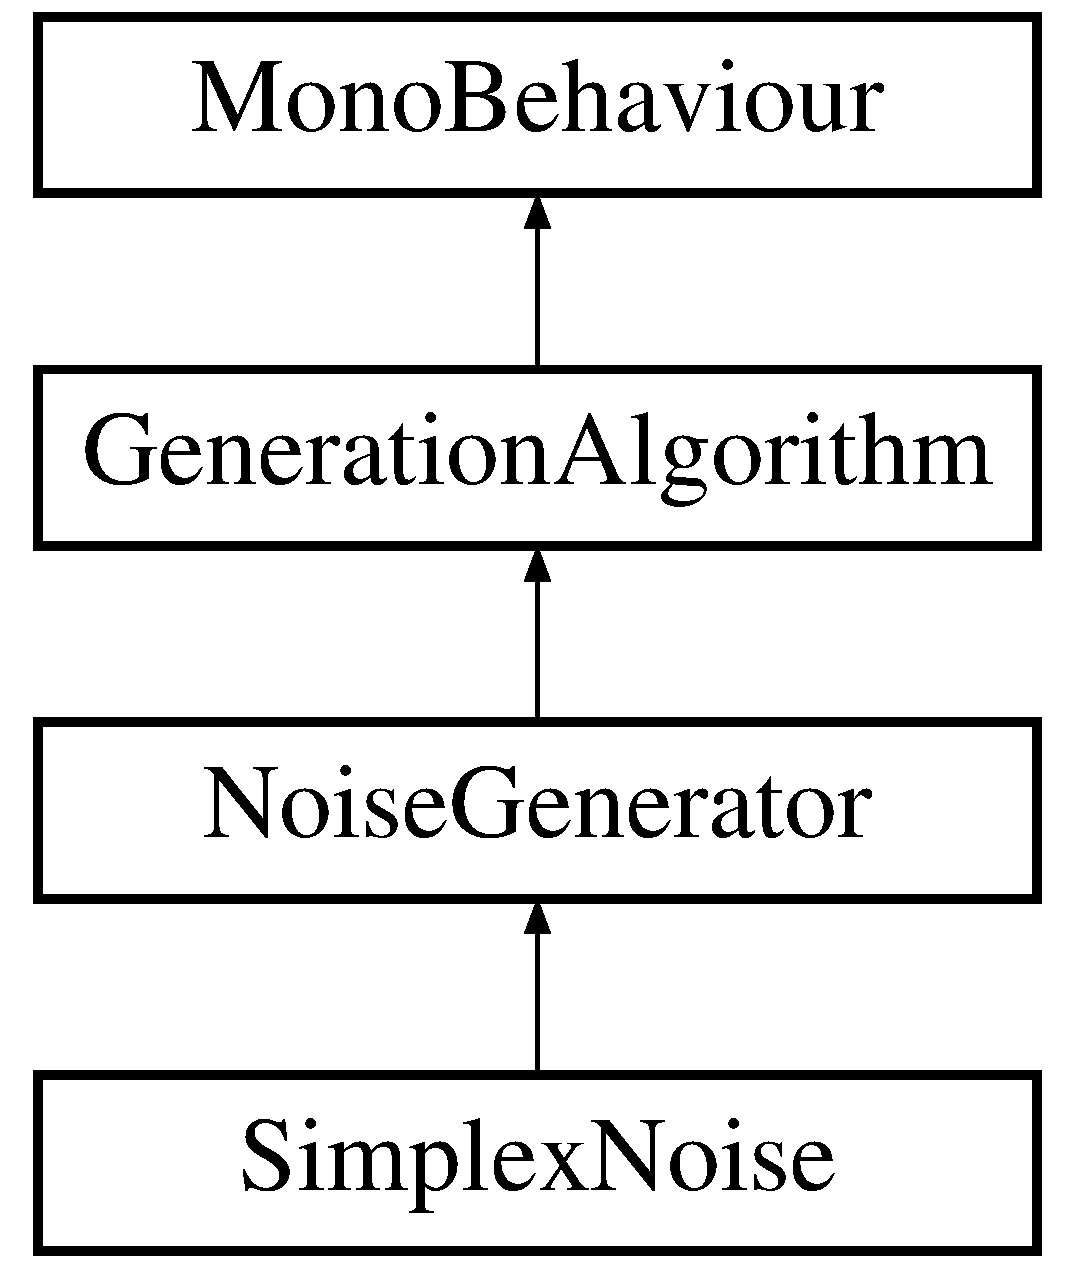
\includegraphics[height=4.000000cm]{class_simplex_noise}
\end{center}
\end{figure}
\subsection*{Classes}
\begin{DoxyCompactItemize}
\item 
class \mbox{\hyperlink{class_simplex_noise_1_1_grad}{Grad}}
\end{DoxyCompactItemize}
\subsection*{Public Member Functions}
\begin{DoxyCompactItemize}
\item 
void \mbox{\hyperlink{class_simplex_noise_a616d1987674e90392904a65c7618c9d4}{init}} (int seed)
\item 
void \mbox{\hyperlink{class_simplex_noise_a151aceb21de5c48ab4b5ff7bf82f6b61}{init}} ()
\item 
float \mbox{\hyperlink{class_simplex_noise_a86ab5f95259f74f43d00a00b695d5755}{noise}} (float xin, float yin)
\item 
override void \mbox{\hyperlink{class_simplex_noise_a43164ec5960921789ce75e83651717cf}{Setup}} ()
\begin{DoxyCompactList}\small\item\em Collects any prerequisites for generation. \end{DoxyCompactList}\item 
override float \mbox{[},\mbox{]} \mbox{\hyperlink{class_simplex_noise_aea5b04e1455da3c6eb8b29deb28a239c}{Generate\+Height\+Map}} (int map\+Width, int map\+Height)
\end{DoxyCompactItemize}
\subsection*{Public Attributes}
\begin{DoxyCompactItemize}
\item 
float \mbox{\hyperlink{class_simplex_noise_aa55bdc3da38443283d578a7eda4987e3}{offsetX}} = 100f
\item 
float \mbox{\hyperlink{class_simplex_noise_ae0fcfbb7ecbb42049f0d80b93a002c10}{offsetY}} = 100f
\item 
\mbox{\hyperlink{class_simplex_noise_1_1_grad}{Grad}} \mbox{[}$\,$\mbox{]} \mbox{\hyperlink{class_simplex_noise_a061de88e8e944eda8e5823a7e4dc7560}{grad3}}
\end{DoxyCompactItemize}
\subsection*{Additional Inherited Members}


\subsection{Member Function Documentation}
\mbox{\Hypertarget{class_simplex_noise_aea5b04e1455da3c6eb8b29deb28a239c}\label{class_simplex_noise_aea5b04e1455da3c6eb8b29deb28a239c}} 
\index{Simplex\+Noise@{Simplex\+Noise}!Generate\+Height\+Map@{Generate\+Height\+Map}}
\index{Generate\+Height\+Map@{Generate\+Height\+Map}!Simplex\+Noise@{Simplex\+Noise}}
\subsubsection{\texorpdfstring{Generate\+Height\+Map()}{GenerateHeightMap()}}
{\footnotesize\ttfamily override float \mbox{[},\mbox{]} Simplex\+Noise.\+Generate\+Height\+Map (\begin{DoxyParamCaption}\item[{int}]{map\+Width,  }\item[{int}]{map\+Height }\end{DoxyParamCaption})\hspace{0.3cm}{\ttfamily [virtual]}}



Implements \mbox{\hyperlink{class_noise_generator_a1d3983a9ad33c2734f373e9f2d8f13d7}{Noise\+Generator}}.

\mbox{\Hypertarget{class_simplex_noise_a616d1987674e90392904a65c7618c9d4}\label{class_simplex_noise_a616d1987674e90392904a65c7618c9d4}} 
\index{Simplex\+Noise@{Simplex\+Noise}!init@{init}}
\index{init@{init}!Simplex\+Noise@{Simplex\+Noise}}
\subsubsection{\texorpdfstring{init()}{init()}\hspace{0.1cm}{\footnotesize\ttfamily [1/2]}}
{\footnotesize\ttfamily void Simplex\+Noise.\+init (\begin{DoxyParamCaption}\item[{int}]{seed }\end{DoxyParamCaption})}

\mbox{\Hypertarget{class_simplex_noise_a151aceb21de5c48ab4b5ff7bf82f6b61}\label{class_simplex_noise_a151aceb21de5c48ab4b5ff7bf82f6b61}} 
\index{Simplex\+Noise@{Simplex\+Noise}!init@{init}}
\index{init@{init}!Simplex\+Noise@{Simplex\+Noise}}
\subsubsection{\texorpdfstring{init()}{init()}\hspace{0.1cm}{\footnotesize\ttfamily [2/2]}}
{\footnotesize\ttfamily void Simplex\+Noise.\+init (\begin{DoxyParamCaption}{ }\end{DoxyParamCaption})}

\mbox{\Hypertarget{class_simplex_noise_a86ab5f95259f74f43d00a00b695d5755}\label{class_simplex_noise_a86ab5f95259f74f43d00a00b695d5755}} 
\index{Simplex\+Noise@{Simplex\+Noise}!noise@{noise}}
\index{noise@{noise}!Simplex\+Noise@{Simplex\+Noise}}
\subsubsection{\texorpdfstring{noise()}{noise()}}
{\footnotesize\ttfamily float Simplex\+Noise.\+noise (\begin{DoxyParamCaption}\item[{float}]{xin,  }\item[{float}]{yin }\end{DoxyParamCaption})}

\mbox{\Hypertarget{class_simplex_noise_a43164ec5960921789ce75e83651717cf}\label{class_simplex_noise_a43164ec5960921789ce75e83651717cf}} 
\index{Simplex\+Noise@{Simplex\+Noise}!Setup@{Setup}}
\index{Setup@{Setup}!Simplex\+Noise@{Simplex\+Noise}}
\subsubsection{\texorpdfstring{Setup()}{Setup()}}
{\footnotesize\ttfamily override void Simplex\+Noise.\+Setup (\begin{DoxyParamCaption}{ }\end{DoxyParamCaption})\hspace{0.3cm}{\ttfamily [virtual]}}



Collects any prerequisites for generation. 



Reimplemented from \mbox{\hyperlink{class_noise_generator_ad87355d424b537a1a4065d525ec18400}{Noise\+Generator}}.



\subsection{Member Data Documentation}
\mbox{\Hypertarget{class_simplex_noise_a061de88e8e944eda8e5823a7e4dc7560}\label{class_simplex_noise_a061de88e8e944eda8e5823a7e4dc7560}} 
\index{Simplex\+Noise@{Simplex\+Noise}!grad3@{grad3}}
\index{grad3@{grad3}!Simplex\+Noise@{Simplex\+Noise}}
\subsubsection{\texorpdfstring{grad3}{grad3}}
{\footnotesize\ttfamily \mbox{\hyperlink{class_simplex_noise_1_1_grad}{Grad}} \mbox{[}$\,$\mbox{]} Simplex\+Noise.\+grad3}

{\bfseries Initial value\+:}
\begin{DoxyCode}
= \{\textcolor{keyword}{new} Grad(1,1),\textcolor{keyword}{new} Grad(-1,1),\textcolor{keyword}{new} Grad(1,-1),\textcolor{keyword}{new} Grad(-1,-1),
                                     \textcolor{keyword}{new} Grad(1,0),\textcolor{keyword}{new} Grad(-1,0),\textcolor{keyword}{new} Grad(1,0),\textcolor{keyword}{new} Grad(-1,0),
                                     \textcolor{keyword}{new} Grad(0,1),\textcolor{keyword}{new} Grad(0,-1),\textcolor{keyword}{new} Grad(0,1),\textcolor{keyword}{new} Grad(0,-1)\}
\end{DoxyCode}
\mbox{\Hypertarget{class_simplex_noise_aa55bdc3da38443283d578a7eda4987e3}\label{class_simplex_noise_aa55bdc3da38443283d578a7eda4987e3}} 
\index{Simplex\+Noise@{Simplex\+Noise}!offsetX@{offsetX}}
\index{offsetX@{offsetX}!Simplex\+Noise@{Simplex\+Noise}}
\subsubsection{\texorpdfstring{offsetX}{offsetX}}
{\footnotesize\ttfamily float Simplex\+Noise.\+offsetX = 100f}

\mbox{\Hypertarget{class_simplex_noise_ae0fcfbb7ecbb42049f0d80b93a002c10}\label{class_simplex_noise_ae0fcfbb7ecbb42049f0d80b93a002c10}} 
\index{Simplex\+Noise@{Simplex\+Noise}!offsetY@{offsetY}}
\index{offsetY@{offsetY}!Simplex\+Noise@{Simplex\+Noise}}
\subsubsection{\texorpdfstring{offsetY}{offsetY}}
{\footnotesize\ttfamily float Simplex\+Noise.\+offsetY = 100f}



The documentation for this class was generated from the following file\+:\begin{DoxyCompactItemize}
\item 
/\+Users/sabienambrose/\+Documents/\+Coding/\+Unity\+Mechanical\+Turk/\+Mechanical\+Turk/\+Assets/\+Scripts/\+Generation/\+Noise/\mbox{\hyperlink{_simplex_noise_8cs}{Simplex\+Noise.\+cs}}\end{DoxyCompactItemize}

\hypertarget{class_simplex_terrain_generator}{}\section{Simplex\+Terrain\+Generator Class Reference}
\label{class_simplex_terrain_generator}\index{Simplex\+Terrain\+Generator@{Simplex\+Terrain\+Generator}}
Inheritance diagram for Simplex\+Terrain\+Generator\+:\begin{figure}[H]
\begin{center}
\leavevmode
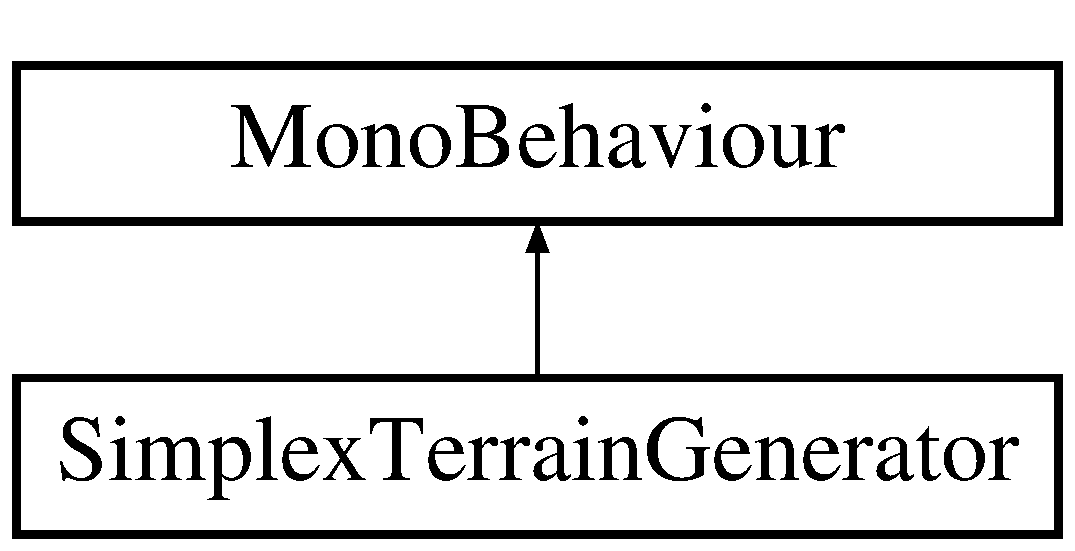
\includegraphics[height=2.000000cm]{class_simplex_terrain_generator}
\end{center}
\end{figure}
\subsection*{Public Member Functions}
\begin{DoxyCompactItemize}
\item 
virtual void \mbox{\hyperlink{class_simplex_terrain_generator_a6d5c45df36f2cc746064d710e35fcd0d}{Generate\+Terrain}} ()
\end{DoxyCompactItemize}
\subsection*{Public Attributes}
\begin{DoxyCompactItemize}
\item 
int \mbox{\hyperlink{class_simplex_terrain_generator_a24f6db85e150e5a30d396aa1cec62e61}{depth}} = 3
\item 
int \mbox{\hyperlink{class_simplex_terrain_generator_acc680a118dccdeb8f2357b13c08563cf}{width}} = 256
\item 
int \mbox{\hyperlink{class_simplex_terrain_generator_a6676586ef4da8c227277362ef96edcc5}{height}} = 256
\item 
float \mbox{\hyperlink{class_simplex_terrain_generator_a5917969e0c0dc92d2775c43bc67ac719}{scale}} = 10f
\item 
float \mbox{\hyperlink{class_simplex_terrain_generator_ac88a461cc43702ec1bc43ac2ec4f4f02}{offsetX}} = 100f
\item 
float \mbox{\hyperlink{class_simplex_terrain_generator_a38e5635574c1ea006575e1425aae3bae}{offsetY}} = 100f
\item 
Texture2D \mbox{\hyperlink{class_simplex_terrain_generator_a4bbaab3f3e220ccd50f53e462ddea0ae}{terrain\+Texture}}
\item 
int \mbox{\hyperlink{class_simplex_terrain_generator_a3d43d13142cafdf8ca3122f2b1445bc1}{seed}} = 0
\end{DoxyCompactItemize}


\subsection{Member Function Documentation}
\mbox{\Hypertarget{class_simplex_terrain_generator_a6d5c45df36f2cc746064d710e35fcd0d}\label{class_simplex_terrain_generator_a6d5c45df36f2cc746064d710e35fcd0d}} 
\index{Simplex\+Terrain\+Generator@{Simplex\+Terrain\+Generator}!Generate\+Terrain@{Generate\+Terrain}}
\index{Generate\+Terrain@{Generate\+Terrain}!Simplex\+Terrain\+Generator@{Simplex\+Terrain\+Generator}}
\subsubsection{\texorpdfstring{Generate\+Terrain()}{GenerateTerrain()}}
{\footnotesize\ttfamily virtual void Simplex\+Terrain\+Generator.\+Generate\+Terrain (\begin{DoxyParamCaption}{ }\end{DoxyParamCaption})\hspace{0.3cm}{\ttfamily [virtual]}}



\subsection{Member Data Documentation}
\mbox{\Hypertarget{class_simplex_terrain_generator_a24f6db85e150e5a30d396aa1cec62e61}\label{class_simplex_terrain_generator_a24f6db85e150e5a30d396aa1cec62e61}} 
\index{Simplex\+Terrain\+Generator@{Simplex\+Terrain\+Generator}!depth@{depth}}
\index{depth@{depth}!Simplex\+Terrain\+Generator@{Simplex\+Terrain\+Generator}}
\subsubsection{\texorpdfstring{depth}{depth}}
{\footnotesize\ttfamily int Simplex\+Terrain\+Generator.\+depth = 3}

\mbox{\Hypertarget{class_simplex_terrain_generator_a6676586ef4da8c227277362ef96edcc5}\label{class_simplex_terrain_generator_a6676586ef4da8c227277362ef96edcc5}} 
\index{Simplex\+Terrain\+Generator@{Simplex\+Terrain\+Generator}!height@{height}}
\index{height@{height}!Simplex\+Terrain\+Generator@{Simplex\+Terrain\+Generator}}
\subsubsection{\texorpdfstring{height}{height}}
{\footnotesize\ttfamily int Simplex\+Terrain\+Generator.\+height = 256}

\mbox{\Hypertarget{class_simplex_terrain_generator_ac88a461cc43702ec1bc43ac2ec4f4f02}\label{class_simplex_terrain_generator_ac88a461cc43702ec1bc43ac2ec4f4f02}} 
\index{Simplex\+Terrain\+Generator@{Simplex\+Terrain\+Generator}!offsetX@{offsetX}}
\index{offsetX@{offsetX}!Simplex\+Terrain\+Generator@{Simplex\+Terrain\+Generator}}
\subsubsection{\texorpdfstring{offsetX}{offsetX}}
{\footnotesize\ttfamily float Simplex\+Terrain\+Generator.\+offsetX = 100f}

\mbox{\Hypertarget{class_simplex_terrain_generator_a38e5635574c1ea006575e1425aae3bae}\label{class_simplex_terrain_generator_a38e5635574c1ea006575e1425aae3bae}} 
\index{Simplex\+Terrain\+Generator@{Simplex\+Terrain\+Generator}!offsetY@{offsetY}}
\index{offsetY@{offsetY}!Simplex\+Terrain\+Generator@{Simplex\+Terrain\+Generator}}
\subsubsection{\texorpdfstring{offsetY}{offsetY}}
{\footnotesize\ttfamily float Simplex\+Terrain\+Generator.\+offsetY = 100f}

\mbox{\Hypertarget{class_simplex_terrain_generator_a5917969e0c0dc92d2775c43bc67ac719}\label{class_simplex_terrain_generator_a5917969e0c0dc92d2775c43bc67ac719}} 
\index{Simplex\+Terrain\+Generator@{Simplex\+Terrain\+Generator}!scale@{scale}}
\index{scale@{scale}!Simplex\+Terrain\+Generator@{Simplex\+Terrain\+Generator}}
\subsubsection{\texorpdfstring{scale}{scale}}
{\footnotesize\ttfamily float Simplex\+Terrain\+Generator.\+scale = 10f}

\mbox{\Hypertarget{class_simplex_terrain_generator_a3d43d13142cafdf8ca3122f2b1445bc1}\label{class_simplex_terrain_generator_a3d43d13142cafdf8ca3122f2b1445bc1}} 
\index{Simplex\+Terrain\+Generator@{Simplex\+Terrain\+Generator}!seed@{seed}}
\index{seed@{seed}!Simplex\+Terrain\+Generator@{Simplex\+Terrain\+Generator}}
\subsubsection{\texorpdfstring{seed}{seed}}
{\footnotesize\ttfamily int Simplex\+Terrain\+Generator.\+seed = 0}

\mbox{\Hypertarget{class_simplex_terrain_generator_a4bbaab3f3e220ccd50f53e462ddea0ae}\label{class_simplex_terrain_generator_a4bbaab3f3e220ccd50f53e462ddea0ae}} 
\index{Simplex\+Terrain\+Generator@{Simplex\+Terrain\+Generator}!terrain\+Texture@{terrain\+Texture}}
\index{terrain\+Texture@{terrain\+Texture}!Simplex\+Terrain\+Generator@{Simplex\+Terrain\+Generator}}
\subsubsection{\texorpdfstring{terrain\+Texture}{terrainTexture}}
{\footnotesize\ttfamily Texture2D Simplex\+Terrain\+Generator.\+terrain\+Texture}

\mbox{\Hypertarget{class_simplex_terrain_generator_acc680a118dccdeb8f2357b13c08563cf}\label{class_simplex_terrain_generator_acc680a118dccdeb8f2357b13c08563cf}} 
\index{Simplex\+Terrain\+Generator@{Simplex\+Terrain\+Generator}!width@{width}}
\index{width@{width}!Simplex\+Terrain\+Generator@{Simplex\+Terrain\+Generator}}
\subsubsection{\texorpdfstring{width}{width}}
{\footnotesize\ttfamily int Simplex\+Terrain\+Generator.\+width = 256}



The documentation for this class was generated from the following file\+:\begin{DoxyCompactItemize}
\item 
/\+Users/sabienambrose/\+Documents/\+Coding/\+Unity\+Mechanical\+Turk/\+Mechanical\+Turk/\+Assets/\+Scripts/\+Generation/\mbox{\hyperlink{_simplex_terrain_generator_8cs}{Simplex\+Terrain\+Generator.\+cs}}\end{DoxyCompactItemize}

\hypertarget{class_spawn_decision}{}\section{Spawn\+Decision Class Reference}
\label{class_spawn_decision}\index{Spawn\+Decision@{Spawn\+Decision}}
Inheritance diagram for Spawn\+Decision\+:\begin{figure}[H]
\begin{center}
\leavevmode
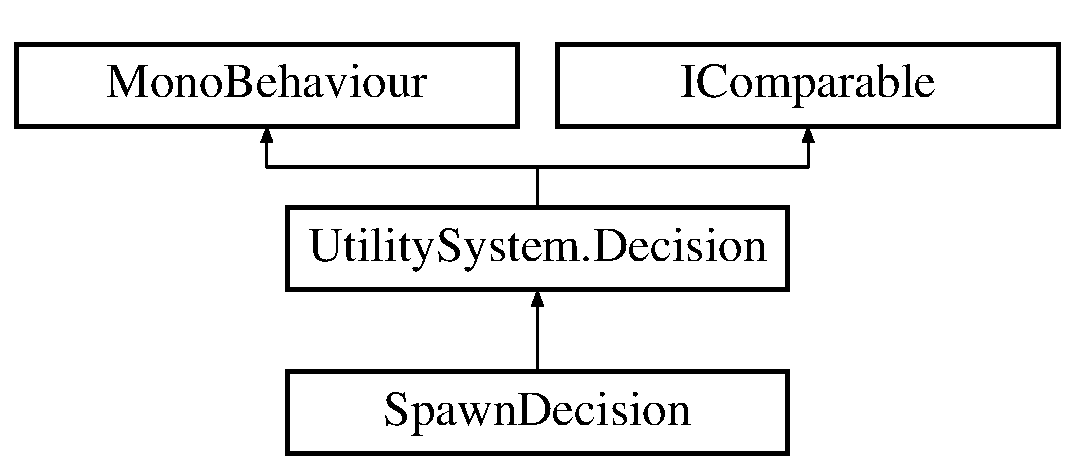
\includegraphics[height=3.000000cm]{class_spawn_decision}
\end{center}
\end{figure}
\subsection*{Public Member Functions}
\begin{DoxyCompactItemize}
\item 
override \mbox{\hyperlink{class_utility_system_1_1_decision_context}{Decision\+Context}} \mbox{\hyperlink{class_spawn_decision_a8c2019e64b2353e9c0eb314cc0e804d7}{Get\+Context}} ()
\item 
override void \mbox{\hyperlink{class_spawn_decision_a7f943d8fd313e6a38f26b223e4b4dba7}{Perform}} ()
\end{DoxyCompactItemize}
\subsection*{Public Attributes}
\begin{DoxyCompactItemize}
\item 
Game\+Object \mbox{\hyperlink{class_spawn_decision_af271fdcf4d0d835a2c4eaf7c9263433d}{object\+To\+Spawn}}
\end{DoxyCompactItemize}


\subsection{Member Function Documentation}
\mbox{\Hypertarget{class_spawn_decision_a8c2019e64b2353e9c0eb314cc0e804d7}\label{class_spawn_decision_a8c2019e64b2353e9c0eb314cc0e804d7}} 
\index{Spawn\+Decision@{Spawn\+Decision}!Get\+Context@{Get\+Context}}
\index{Get\+Context@{Get\+Context}!Spawn\+Decision@{Spawn\+Decision}}
\subsubsection{\texorpdfstring{Get\+Context()}{GetContext()}}
{\footnotesize\ttfamily override \mbox{\hyperlink{class_utility_system_1_1_decision_context}{Decision\+Context}} Spawn\+Decision.\+Get\+Context (\begin{DoxyParamCaption}{ }\end{DoxyParamCaption})\hspace{0.3cm}{\ttfamily [virtual]}}



Implements \mbox{\hyperlink{class_utility_system_1_1_decision_a46ba8cac39f52c630897a24f2bde6b07}{Utility\+System.\+Decision}}.

\mbox{\Hypertarget{class_spawn_decision_a7f943d8fd313e6a38f26b223e4b4dba7}\label{class_spawn_decision_a7f943d8fd313e6a38f26b223e4b4dba7}} 
\index{Spawn\+Decision@{Spawn\+Decision}!Perform@{Perform}}
\index{Perform@{Perform}!Spawn\+Decision@{Spawn\+Decision}}
\subsubsection{\texorpdfstring{Perform()}{Perform()}}
{\footnotesize\ttfamily override void Spawn\+Decision.\+Perform (\begin{DoxyParamCaption}{ }\end{DoxyParamCaption})\hspace{0.3cm}{\ttfamily [virtual]}}



Implements \mbox{\hyperlink{class_utility_system_1_1_decision_a055dcaafb617365bc8b16bb9acba6575}{Utility\+System.\+Decision}}.



\subsection{Member Data Documentation}
\mbox{\Hypertarget{class_spawn_decision_af271fdcf4d0d835a2c4eaf7c9263433d}\label{class_spawn_decision_af271fdcf4d0d835a2c4eaf7c9263433d}} 
\index{Spawn\+Decision@{Spawn\+Decision}!object\+To\+Spawn@{object\+To\+Spawn}}
\index{object\+To\+Spawn@{object\+To\+Spawn}!Spawn\+Decision@{Spawn\+Decision}}
\subsubsection{\texorpdfstring{object\+To\+Spawn}{objectToSpawn}}
{\footnotesize\ttfamily Game\+Object Spawn\+Decision.\+object\+To\+Spawn}



The documentation for this class was generated from the following file\+:\begin{DoxyCompactItemize}
\item 
/\+Users/sabienambrose/\+Documents/\+Coding/\+Unity\+Mechanical\+Turk/\+Mechanical\+Turk/\+Assets/\+Scripts/\+Pathfinding/\+Utility/\+Decisions/\mbox{\hyperlink{_spawn_decision_8cs}{Spawn\+Decision.\+cs}}\end{DoxyCompactItemize}

\hypertarget{struct_square_grid_params}{}\section{Square\+Grid\+Params Struct Reference}
\label{struct_square_grid_params}\index{Square\+Grid\+Params@{Square\+Grid\+Params}}
\subsection*{Public Member Functions}
\begin{DoxyCompactItemize}
\item 
\mbox{\hyperlink{struct_square_grid_params_a0a79f3a8860e1efdf383128bda2171da}{Square\+Grid\+Params}} (\mbox{\hyperlink{class_poly_grid}{Poly\+Grid}} source)
\item 
Vector2 \mbox{\hyperlink{struct_square_grid_params_a251c90bf64a7b0d0ea2b8f572910d912}{Get\+Face\+Dimensions}} ()
\item 
Vector2\+Int \mbox{\hyperlink{struct_square_grid_params_a22366f3bf69926bad2d21e5967112495}{Num\+Vertices}} ()
\end{DoxyCompactItemize}
\subsection*{Public Attributes}
\begin{DoxyCompactItemize}
\item 
Vector2 \mbox{\hyperlink{struct_square_grid_params_ad205c7b2c188015047991266aa64eadc}{Dimensions}}
\item 
Vector2\+Int \mbox{\hyperlink{struct_square_grid_params_af19744bb944c6a51cacd30c9d3ac9059}{Faces\+Per\+Side}}
\end{DoxyCompactItemize}


\subsection{Constructor \& Destructor Documentation}
\mbox{\Hypertarget{struct_square_grid_params_a0a79f3a8860e1efdf383128bda2171da}\label{struct_square_grid_params_a0a79f3a8860e1efdf383128bda2171da}} 
\index{Square\+Grid\+Params@{Square\+Grid\+Params}!Square\+Grid\+Params@{Square\+Grid\+Params}}
\index{Square\+Grid\+Params@{Square\+Grid\+Params}!Square\+Grid\+Params@{Square\+Grid\+Params}}
\subsubsection{\texorpdfstring{Square\+Grid\+Params()}{SquareGridParams()}}
{\footnotesize\ttfamily Square\+Grid\+Params.\+Square\+Grid\+Params (\begin{DoxyParamCaption}\item[{\mbox{\hyperlink{class_poly_grid}{Poly\+Grid}}}]{source }\end{DoxyParamCaption})}



\subsection{Member Function Documentation}
\mbox{\Hypertarget{struct_square_grid_params_a251c90bf64a7b0d0ea2b8f572910d912}\label{struct_square_grid_params_a251c90bf64a7b0d0ea2b8f572910d912}} 
\index{Square\+Grid\+Params@{Square\+Grid\+Params}!Get\+Face\+Dimensions@{Get\+Face\+Dimensions}}
\index{Get\+Face\+Dimensions@{Get\+Face\+Dimensions}!Square\+Grid\+Params@{Square\+Grid\+Params}}
\subsubsection{\texorpdfstring{Get\+Face\+Dimensions()}{GetFaceDimensions()}}
{\footnotesize\ttfamily Vector2 Square\+Grid\+Params.\+Get\+Face\+Dimensions (\begin{DoxyParamCaption}{ }\end{DoxyParamCaption})}

\mbox{\Hypertarget{struct_square_grid_params_a22366f3bf69926bad2d21e5967112495}\label{struct_square_grid_params_a22366f3bf69926bad2d21e5967112495}} 
\index{Square\+Grid\+Params@{Square\+Grid\+Params}!Num\+Vertices@{Num\+Vertices}}
\index{Num\+Vertices@{Num\+Vertices}!Square\+Grid\+Params@{Square\+Grid\+Params}}
\subsubsection{\texorpdfstring{Num\+Vertices()}{NumVertices()}}
{\footnotesize\ttfamily Vector2\+Int Square\+Grid\+Params.\+Num\+Vertices (\begin{DoxyParamCaption}{ }\end{DoxyParamCaption})}



\subsection{Member Data Documentation}
\mbox{\Hypertarget{struct_square_grid_params_ad205c7b2c188015047991266aa64eadc}\label{struct_square_grid_params_ad205c7b2c188015047991266aa64eadc}} 
\index{Square\+Grid\+Params@{Square\+Grid\+Params}!Dimensions@{Dimensions}}
\index{Dimensions@{Dimensions}!Square\+Grid\+Params@{Square\+Grid\+Params}}
\subsubsection{\texorpdfstring{Dimensions}{Dimensions}}
{\footnotesize\ttfamily Vector2 Square\+Grid\+Params.\+Dimensions}

\mbox{\Hypertarget{struct_square_grid_params_af19744bb944c6a51cacd30c9d3ac9059}\label{struct_square_grid_params_af19744bb944c6a51cacd30c9d3ac9059}} 
\index{Square\+Grid\+Params@{Square\+Grid\+Params}!Faces\+Per\+Side@{Faces\+Per\+Side}}
\index{Faces\+Per\+Side@{Faces\+Per\+Side}!Square\+Grid\+Params@{Square\+Grid\+Params}}
\subsubsection{\texorpdfstring{Faces\+Per\+Side}{FacesPerSide}}
{\footnotesize\ttfamily Vector2\+Int Square\+Grid\+Params.\+Faces\+Per\+Side}



The documentation for this struct was generated from the following file\+:\begin{DoxyCompactItemize}
\item 
/\+Users/sabienambrose/\+Documents/\+Coding/\+Unity\+Mechanical\+Turk/\+Mechanical\+Turk/\+Assets/\+Scripts/\+Util/\+Containers/\+Graphs/\+Grids/\mbox{\hyperlink{_grid_factory_8cs}{Grid\+Factory.\+cs}}\end{DoxyCompactItemize}

\hypertarget{class_terrain_generator}{}\section{Terrain\+Generator Class Reference}
\label{class_terrain_generator}\index{Terrain\+Generator@{Terrain\+Generator}}
Inheritance diagram for Terrain\+Generator\+:\begin{figure}[H]
\begin{center}
\leavevmode
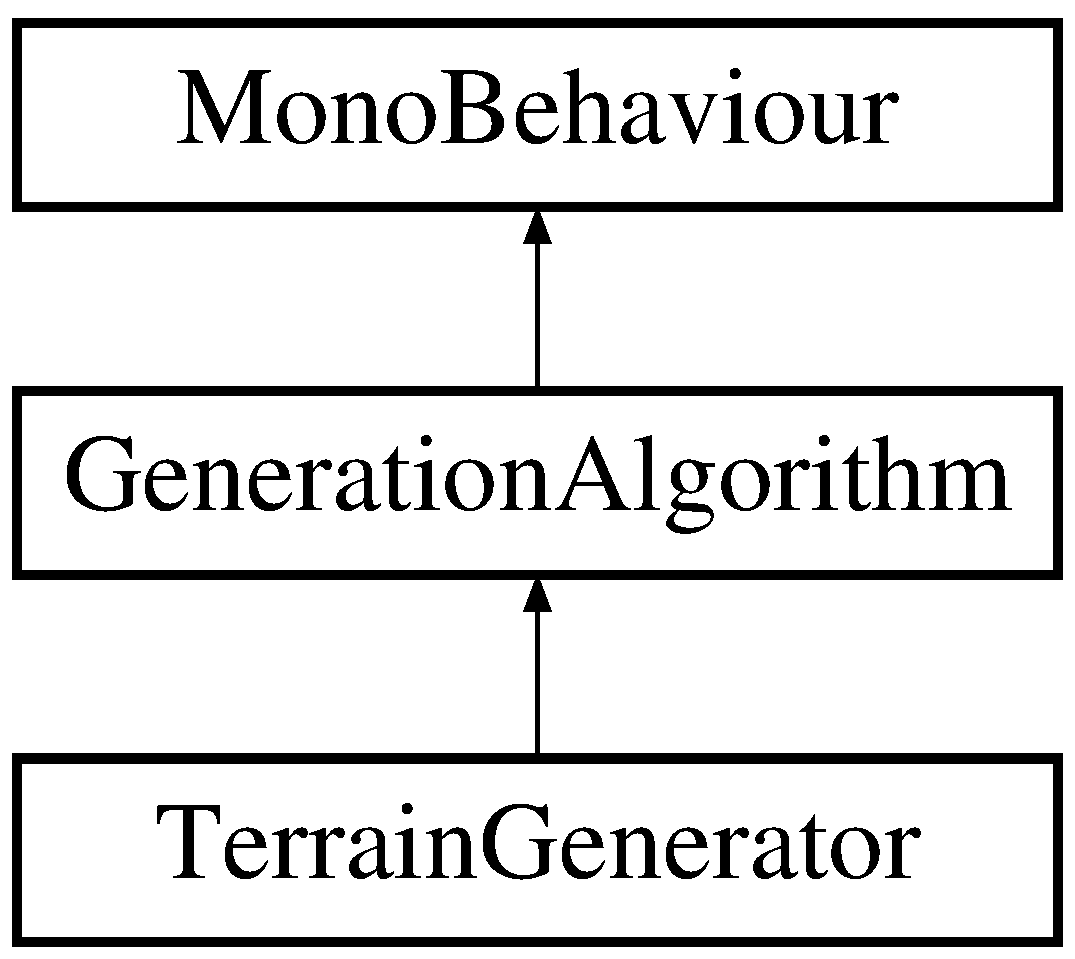
\includegraphics[height=3.000000cm]{class_terrain_generator}
\end{center}
\end{figure}
\subsection*{Public Member Functions}
\begin{DoxyCompactItemize}
\item 
override bool \mbox{\hyperlink{class_terrain_generator_aecef659ebcfc0b012f4f8eb42e11f337}{Can\+Generate}} ()
\begin{DoxyCompactList}\small\item\em Checks to see if generation prerequisites are met. \end{DoxyCompactList}\item 
override void \mbox{\hyperlink{class_terrain_generator_ada250260b370382c1ba5cad243a67f10}{Setup}} ()
\begin{DoxyCompactList}\small\item\em Collects any prerequisites for generation. \end{DoxyCompactList}\item 
override void \mbox{\hyperlink{class_terrain_generator_ace92d2a3406204b124c51e91f68a0aec}{Generate}} ()
\item 
virtual void \mbox{\hyperlink{class_terrain_generator_ad39c135988960e8e12ea5bd36569336f}{Generate\+Biomes}} ()
\item 
virtual void \mbox{\hyperlink{class_terrain_generator_a9bbb5a5cfa43d7f38a8ef881b966ee26}{Apply\+Height\+Map}} ()
\begin{DoxyCompactList}\small\item\em Assign height values to the terrain \end{DoxyCompactList}\item 
virtual void \mbox{\hyperlink{class_terrain_generator_a8aac3ecefc24ee4f4018994ae29a1bba}{Apply\+Biome\+Map}} ()
\end{DoxyCompactItemize}
\subsection*{Public Attributes}
\begin{DoxyCompactItemize}
\item 
\mbox{\hyperlink{class_noise_generator}{Noise\+Generator}} \mbox{\hyperlink{class_terrain_generator_a71c54a5bcb57410020cacf5a3ef8d490}{height\+Map\+Generator}}
\item 
\mbox{\hyperlink{class_biome_generator}{Biome\+Generator}} \mbox{\hyperlink{class_terrain_generator_ac4a6046f1aa01960502dae2faa7bbf8d}{biome\+Generator}}
\item 
float \mbox{\hyperlink{class_terrain_generator_a6439dffc9f1649c25f1439b9edf7d0ac}{height\+Scale}} = 1f
\item 
\mbox{\hyperlink{class_noise_map}{Noise\+Map}} \mbox{\hyperlink{class_terrain_generator_acc1ef38d028ff5a3bfd4288c0ae4dd1c}{height\+Map}}
\item 
Terrain \mbox{\hyperlink{class_terrain_generator_a1f609c5d9b82c0976d0efb81120516ee}{terrain}}
\item 
Texture2D \mbox{\hyperlink{class_terrain_generator_ad1cc3b94c469294950cb6a900fc8e86b}{biome\+Texture}}
\end{DoxyCompactItemize}


\subsection{Member Function Documentation}
\mbox{\Hypertarget{class_terrain_generator_a8aac3ecefc24ee4f4018994ae29a1bba}\label{class_terrain_generator_a8aac3ecefc24ee4f4018994ae29a1bba}} 
\index{Terrain\+Generator@{Terrain\+Generator}!Apply\+Biome\+Map@{Apply\+Biome\+Map}}
\index{Apply\+Biome\+Map@{Apply\+Biome\+Map}!Terrain\+Generator@{Terrain\+Generator}}
\subsubsection{\texorpdfstring{Apply\+Biome\+Map()}{ApplyBiomeMap()}}
{\footnotesize\ttfamily virtual void Terrain\+Generator.\+Apply\+Biome\+Map (\begin{DoxyParamCaption}{ }\end{DoxyParamCaption})\hspace{0.3cm}{\ttfamily [virtual]}}

\mbox{\Hypertarget{class_terrain_generator_a9bbb5a5cfa43d7f38a8ef881b966ee26}\label{class_terrain_generator_a9bbb5a5cfa43d7f38a8ef881b966ee26}} 
\index{Terrain\+Generator@{Terrain\+Generator}!Apply\+Height\+Map@{Apply\+Height\+Map}}
\index{Apply\+Height\+Map@{Apply\+Height\+Map}!Terrain\+Generator@{Terrain\+Generator}}
\subsubsection{\texorpdfstring{Apply\+Height\+Map()}{ApplyHeightMap()}}
{\footnotesize\ttfamily virtual void Terrain\+Generator.\+Apply\+Height\+Map (\begin{DoxyParamCaption}{ }\end{DoxyParamCaption})\hspace{0.3cm}{\ttfamily [virtual]}}



Assign height values to the terrain 

\mbox{\Hypertarget{class_terrain_generator_aecef659ebcfc0b012f4f8eb42e11f337}\label{class_terrain_generator_aecef659ebcfc0b012f4f8eb42e11f337}} 
\index{Terrain\+Generator@{Terrain\+Generator}!Can\+Generate@{Can\+Generate}}
\index{Can\+Generate@{Can\+Generate}!Terrain\+Generator@{Terrain\+Generator}}
\subsubsection{\texorpdfstring{Can\+Generate()}{CanGenerate()}}
{\footnotesize\ttfamily override bool Terrain\+Generator.\+Can\+Generate (\begin{DoxyParamCaption}{ }\end{DoxyParamCaption})\hspace{0.3cm}{\ttfamily [virtual]}}



Checks to see if generation prerequisites are met. 

\begin{DoxyReturn}{Returns}
true if ready for generation.
\end{DoxyReturn}


Implements \mbox{\hyperlink{class_generation_algorithm_af7d03e24e3b7fecfe2ae43f06915986d}{Generation\+Algorithm}}.

\mbox{\Hypertarget{class_terrain_generator_ace92d2a3406204b124c51e91f68a0aec}\label{class_terrain_generator_ace92d2a3406204b124c51e91f68a0aec}} 
\index{Terrain\+Generator@{Terrain\+Generator}!Generate@{Generate}}
\index{Generate@{Generate}!Terrain\+Generator@{Terrain\+Generator}}
\subsubsection{\texorpdfstring{Generate()}{Generate()}}
{\footnotesize\ttfamily override void Terrain\+Generator.\+Generate (\begin{DoxyParamCaption}{ }\end{DoxyParamCaption})\hspace{0.3cm}{\ttfamily [virtual]}}



Implements \mbox{\hyperlink{class_generation_algorithm_ac2df20f7751c1b480ab958791d5c7d41}{Generation\+Algorithm}}.

\mbox{\Hypertarget{class_terrain_generator_ad39c135988960e8e12ea5bd36569336f}\label{class_terrain_generator_ad39c135988960e8e12ea5bd36569336f}} 
\index{Terrain\+Generator@{Terrain\+Generator}!Generate\+Biomes@{Generate\+Biomes}}
\index{Generate\+Biomes@{Generate\+Biomes}!Terrain\+Generator@{Terrain\+Generator}}
\subsubsection{\texorpdfstring{Generate\+Biomes()}{GenerateBiomes()}}
{\footnotesize\ttfamily virtual void Terrain\+Generator.\+Generate\+Biomes (\begin{DoxyParamCaption}{ }\end{DoxyParamCaption})\hspace{0.3cm}{\ttfamily [virtual]}}

\mbox{\Hypertarget{class_terrain_generator_ada250260b370382c1ba5cad243a67f10}\label{class_terrain_generator_ada250260b370382c1ba5cad243a67f10}} 
\index{Terrain\+Generator@{Terrain\+Generator}!Setup@{Setup}}
\index{Setup@{Setup}!Terrain\+Generator@{Terrain\+Generator}}
\subsubsection{\texorpdfstring{Setup()}{Setup()}}
{\footnotesize\ttfamily override void Terrain\+Generator.\+Setup (\begin{DoxyParamCaption}{ }\end{DoxyParamCaption})\hspace{0.3cm}{\ttfamily [virtual]}}



Collects any prerequisites for generation. 



Implements \mbox{\hyperlink{class_generation_algorithm_a5e891b08f0c1d8f4ccc9ad06667691ec}{Generation\+Algorithm}}.



\subsection{Member Data Documentation}
\mbox{\Hypertarget{class_terrain_generator_ac4a6046f1aa01960502dae2faa7bbf8d}\label{class_terrain_generator_ac4a6046f1aa01960502dae2faa7bbf8d}} 
\index{Terrain\+Generator@{Terrain\+Generator}!biome\+Generator@{biome\+Generator}}
\index{biome\+Generator@{biome\+Generator}!Terrain\+Generator@{Terrain\+Generator}}
\subsubsection{\texorpdfstring{biome\+Generator}{biomeGenerator}}
{\footnotesize\ttfamily \mbox{\hyperlink{class_biome_generator}{Biome\+Generator}} Terrain\+Generator.\+biome\+Generator}

\mbox{\Hypertarget{class_terrain_generator_ad1cc3b94c469294950cb6a900fc8e86b}\label{class_terrain_generator_ad1cc3b94c469294950cb6a900fc8e86b}} 
\index{Terrain\+Generator@{Terrain\+Generator}!biome\+Texture@{biome\+Texture}}
\index{biome\+Texture@{biome\+Texture}!Terrain\+Generator@{Terrain\+Generator}}
\subsubsection{\texorpdfstring{biome\+Texture}{biomeTexture}}
{\footnotesize\ttfamily Texture2D Terrain\+Generator.\+biome\+Texture}

\mbox{\Hypertarget{class_terrain_generator_acc1ef38d028ff5a3bfd4288c0ae4dd1c}\label{class_terrain_generator_acc1ef38d028ff5a3bfd4288c0ae4dd1c}} 
\index{Terrain\+Generator@{Terrain\+Generator}!height\+Map@{height\+Map}}
\index{height\+Map@{height\+Map}!Terrain\+Generator@{Terrain\+Generator}}
\subsubsection{\texorpdfstring{height\+Map}{heightMap}}
{\footnotesize\ttfamily \mbox{\hyperlink{class_noise_map}{Noise\+Map}} Terrain\+Generator.\+height\+Map}

\mbox{\Hypertarget{class_terrain_generator_a71c54a5bcb57410020cacf5a3ef8d490}\label{class_terrain_generator_a71c54a5bcb57410020cacf5a3ef8d490}} 
\index{Terrain\+Generator@{Terrain\+Generator}!height\+Map\+Generator@{height\+Map\+Generator}}
\index{height\+Map\+Generator@{height\+Map\+Generator}!Terrain\+Generator@{Terrain\+Generator}}
\subsubsection{\texorpdfstring{height\+Map\+Generator}{heightMapGenerator}}
{\footnotesize\ttfamily \mbox{\hyperlink{class_noise_generator}{Noise\+Generator}} Terrain\+Generator.\+height\+Map\+Generator}

\mbox{\Hypertarget{class_terrain_generator_a6439dffc9f1649c25f1439b9edf7d0ac}\label{class_terrain_generator_a6439dffc9f1649c25f1439b9edf7d0ac}} 
\index{Terrain\+Generator@{Terrain\+Generator}!height\+Scale@{height\+Scale}}
\index{height\+Scale@{height\+Scale}!Terrain\+Generator@{Terrain\+Generator}}
\subsubsection{\texorpdfstring{height\+Scale}{heightScale}}
{\footnotesize\ttfamily float Terrain\+Generator.\+height\+Scale = 1f}

\mbox{\Hypertarget{class_terrain_generator_a1f609c5d9b82c0976d0efb81120516ee}\label{class_terrain_generator_a1f609c5d9b82c0976d0efb81120516ee}} 
\index{Terrain\+Generator@{Terrain\+Generator}!terrain@{terrain}}
\index{terrain@{terrain}!Terrain\+Generator@{Terrain\+Generator}}
\subsubsection{\texorpdfstring{terrain}{terrain}}
{\footnotesize\ttfamily Terrain Terrain\+Generator.\+terrain}



The documentation for this class was generated from the following file\+:\begin{DoxyCompactItemize}
\item 
/\+Users/sabienambrose/\+Documents/\+Coding/\+Unity\+Mechanical\+Turk/\+Mechanical\+Turk/\+Assets/\+Scripts/\+Generation/\mbox{\hyperlink{_terrain_generator_8cs}{Terrain\+Generator.\+cs}}\end{DoxyCompactItemize}

\hypertarget{struct_terrain_type}{}\section{Terrain\+Type Struct Reference}
\label{struct_terrain_type}\index{Terrain\+Type@{Terrain\+Type}}
\subsection*{Public Attributes}
\begin{DoxyCompactItemize}
\item 
string \mbox{\hyperlink{struct_terrain_type_ac119720a6896f5caa7c9fa7fad76ea4c}{name}}
\item 
float \mbox{\hyperlink{struct_terrain_type_ad603fa27bc1652ffb7a92ceee8e218a6}{height}}
\item 
Color \mbox{\hyperlink{struct_terrain_type_ada6b1e20a76513d417966f41ebdf3146}{colour}}
\end{DoxyCompactItemize}


\subsection{Member Data Documentation}
\mbox{\Hypertarget{struct_terrain_type_ada6b1e20a76513d417966f41ebdf3146}\label{struct_terrain_type_ada6b1e20a76513d417966f41ebdf3146}} 
\index{Terrain\+Type@{Terrain\+Type}!colour@{colour}}
\index{colour@{colour}!Terrain\+Type@{Terrain\+Type}}
\subsubsection{\texorpdfstring{colour}{colour}}
{\footnotesize\ttfamily Color Terrain\+Type.\+colour}

\mbox{\Hypertarget{struct_terrain_type_ad603fa27bc1652ffb7a92ceee8e218a6}\label{struct_terrain_type_ad603fa27bc1652ffb7a92ceee8e218a6}} 
\index{Terrain\+Type@{Terrain\+Type}!height@{height}}
\index{height@{height}!Terrain\+Type@{Terrain\+Type}}
\subsubsection{\texorpdfstring{height}{height}}
{\footnotesize\ttfamily float Terrain\+Type.\+height}

\mbox{\Hypertarget{struct_terrain_type_ac119720a6896f5caa7c9fa7fad76ea4c}\label{struct_terrain_type_ac119720a6896f5caa7c9fa7fad76ea4c}} 
\index{Terrain\+Type@{Terrain\+Type}!name@{name}}
\index{name@{name}!Terrain\+Type@{Terrain\+Type}}
\subsubsection{\texorpdfstring{name}{name}}
{\footnotesize\ttfamily string Terrain\+Type.\+name}



The documentation for this struct was generated from the following file\+:\begin{DoxyCompactItemize}
\item 
/\+Users/sabienambrose/\+Documents/\+Coding/\+Unity\+Mechanical\+Turk/\+Mechanical\+Turk/\+Assets/\+Scripts/\+Generation/\mbox{\hyperlink{_map_generator_8cs}{Map\+Generator.\+cs}}\end{DoxyCompactItemize}

\hypertarget{class_tile_a_star}{}\section{Tile\+A\+Star Class Reference}
\label{class_tile_a_star}\index{Tile\+A\+Star@{Tile\+A\+Star}}
Inheritance diagram for Tile\+A\+Star\+:\begin{figure}[H]
\begin{center}
\leavevmode
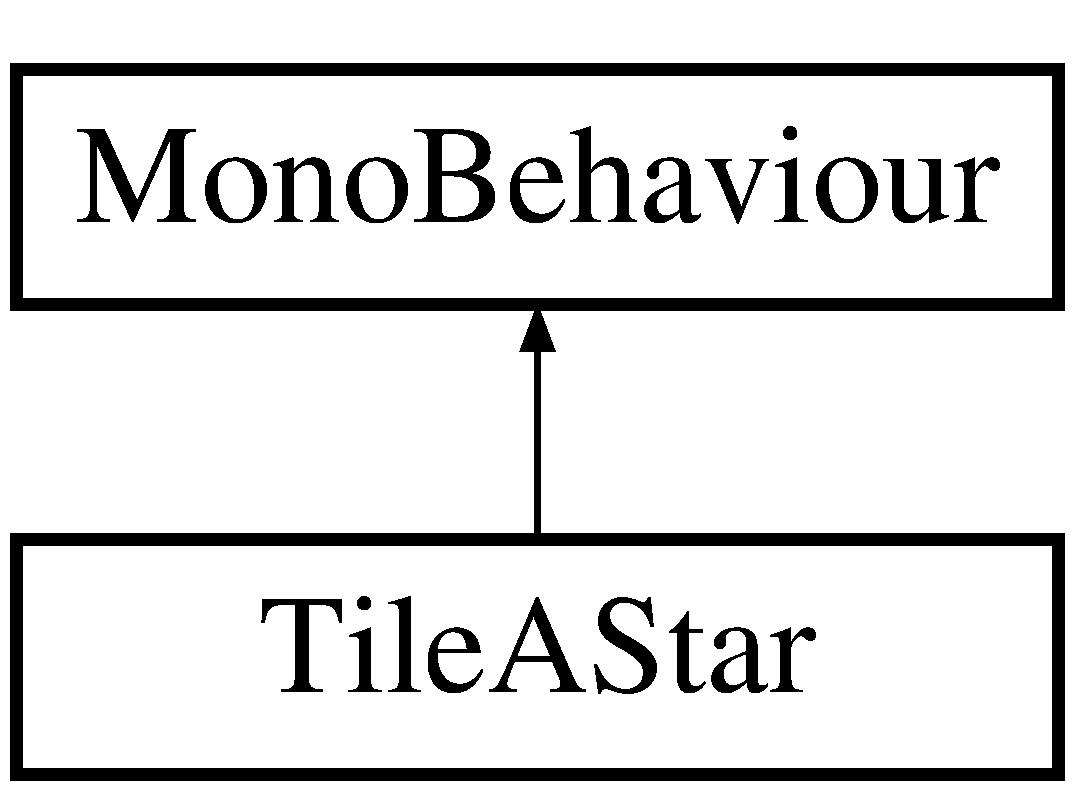
\includegraphics[height=2.000000cm]{class_tile_a_star}
\end{center}
\end{figure}
\subsection*{Public Member Functions}
\begin{DoxyCompactItemize}
\item 
bool \mbox{\hyperlink{class_tile_a_star_a8d7f8af9a007aac6b21553c6d3de0fc6}{Find\+Agent\+Path}} (Game\+Object agent, Transform goal)
\item 
void \mbox{\hyperlink{class_tile_a_star_ae6c2de8ee7160c0d91a28186671717a9}{Init}} ()
\item 
bool \mbox{\hyperlink{class_tile_a_star_a36a0c7fdd0eb1b5189c9e89b2508a714}{Find\+Path}} ()
\begin{DoxyCompactList}\small\item\em Performs A\+Star on a tile grid. \end{DoxyCompactList}\item 
void \mbox{\hyperlink{class_tile_a_star_a287ce910694b2dbf17b03a136557fc26}{Add\+Priority\+Node}} (\mbox{\hyperlink{struct_int_point}{Int\+Point}} node)
\item 
void \mbox{\hyperlink{class_tile_a_star_aff4c93fd2de21b4a7edb156beb76eb2b}{Close\+Node}} (\mbox{\hyperlink{struct_int_point}{Int\+Point}} node)
\item 
int \mbox{\hyperlink{class_tile_a_star_a039b9366e5d285b1c1efe7d3472f80c6}{Get\+Num\+Open\+Nodes}} ()
\item 
\mbox{\hyperlink{struct_int_point}{Int\+Point}} \mbox{\hyperlink{class_tile_a_star_aaf9df73761ac2b7010ec6f85c3cc1b41}{Get\+Smallest\+Open\+Node}} ()
\begin{DoxyCompactList}\small\item\em Finds the smallest open node using the estimated total cost. \end{DoxyCompactList}\item 
List$<$ \mbox{\hyperlink{interface_i_connection}{I\+Connection}}$<$ \mbox{\hyperlink{struct_int_point}{Int\+Point}} $>$ $>$ \mbox{\hyperlink{class_tile_a_star_ab1b21f2b31d816092c4ae9c04d300b96}{Get\+Path\+Connections}} ()
\item 
List$<$ Vector3 $>$ \mbox{\hyperlink{class_tile_a_star_a4566e80f8a54eb58308274acd8d68f7f}{Get\+Path}} ()
\begin{DoxyCompactList}\small\item\em Returns list of path points in world coordinates. \end{DoxyCompactList}\item 
void \mbox{\hyperlink{class_tile_a_star_a2c93e6c430d2b7cc8bde48f8f9b6c1d1}{Smooth\+Path}} ()
\item 
void \mbox{\hyperlink{class_tile_a_star_a5c24481a7825311a5d5b285f3d8368e4}{Clear}} ()
\item 
void \mbox{\hyperlink{class_tile_a_star_af74b5cf47adcbb877850cc5879a94b76}{On\+Draw\+Gizmos}} ()
\end{DoxyCompactItemize}
\subsection*{Public Attributes}
\begin{DoxyCompactItemize}
\item 
\mbox{\hyperlink{class_path_smoother}{Path\+Smoother}} \mbox{\hyperlink{class_tile_a_star_a8be7b45c974dd14d03e25c9b14c68bbb}{path\+Smoother}}
\item 
bool \mbox{\hyperlink{class_tile_a_star_ad703b3c8e7da213a77f48aac7a31a584}{draw\+Unsmoothed\+Path}} = false
\item 
\mbox{\hyperlink{class_tile_world}{Tile\+World}} \mbox{\hyperlink{class_tile_a_star_af591c7bc11527c0fbd3391de4662b5fd}{tile\+World}}
\item 
\mbox{\hyperlink{class_tile_graph}{Tile\+Graph}} \mbox{\hyperlink{class_tile_a_star_ae61928ec47179b3c2eb0970a1fa357f0}{tile\+Graph}}
\item 
Transform \mbox{\hyperlink{class_tile_a_star_ac069531b4fcda54823e312cad7dc48b3}{start\+Transform}}
\item 
Transform \mbox{\hyperlink{class_tile_a_star_aaa0642f5a2f60fb38db368e8681f561d}{goal\+Transform}}
\item 
\mbox{\hyperlink{class_heuristic}{Heuristic}}$<$ \mbox{\hyperlink{struct_int_point}{Int\+Point}} $>$ \mbox{\hyperlink{class_tile_a_star_a002f676fe798cb5dba26e360fac164b9}{heuristic}}
\end{DoxyCompactItemize}


\subsection{Member Function Documentation}
\mbox{\Hypertarget{class_tile_a_star_a287ce910694b2dbf17b03a136557fc26}\label{class_tile_a_star_a287ce910694b2dbf17b03a136557fc26}} 
\index{Tile\+A\+Star@{Tile\+A\+Star}!Add\+Priority\+Node@{Add\+Priority\+Node}}
\index{Add\+Priority\+Node@{Add\+Priority\+Node}!Tile\+A\+Star@{Tile\+A\+Star}}
\subsubsection{\texorpdfstring{Add\+Priority\+Node()}{AddPriorityNode()}}
{\footnotesize\ttfamily void Tile\+A\+Star.\+Add\+Priority\+Node (\begin{DoxyParamCaption}\item[{\mbox{\hyperlink{struct_int_point}{Int\+Point}}}]{node }\end{DoxyParamCaption})}

\mbox{\Hypertarget{class_tile_a_star_a5c24481a7825311a5d5b285f3d8368e4}\label{class_tile_a_star_a5c24481a7825311a5d5b285f3d8368e4}} 
\index{Tile\+A\+Star@{Tile\+A\+Star}!Clear@{Clear}}
\index{Clear@{Clear}!Tile\+A\+Star@{Tile\+A\+Star}}
\subsubsection{\texorpdfstring{Clear()}{Clear()}}
{\footnotesize\ttfamily void Tile\+A\+Star.\+Clear (\begin{DoxyParamCaption}{ }\end{DoxyParamCaption})}

\mbox{\Hypertarget{class_tile_a_star_aff4c93fd2de21b4a7edb156beb76eb2b}\label{class_tile_a_star_aff4c93fd2de21b4a7edb156beb76eb2b}} 
\index{Tile\+A\+Star@{Tile\+A\+Star}!Close\+Node@{Close\+Node}}
\index{Close\+Node@{Close\+Node}!Tile\+A\+Star@{Tile\+A\+Star}}
\subsubsection{\texorpdfstring{Close\+Node()}{CloseNode()}}
{\footnotesize\ttfamily void Tile\+A\+Star.\+Close\+Node (\begin{DoxyParamCaption}\item[{\mbox{\hyperlink{struct_int_point}{Int\+Point}}}]{node }\end{DoxyParamCaption})}

\mbox{\Hypertarget{class_tile_a_star_a8d7f8af9a007aac6b21553c6d3de0fc6}\label{class_tile_a_star_a8d7f8af9a007aac6b21553c6d3de0fc6}} 
\index{Tile\+A\+Star@{Tile\+A\+Star}!Find\+Agent\+Path@{Find\+Agent\+Path}}
\index{Find\+Agent\+Path@{Find\+Agent\+Path}!Tile\+A\+Star@{Tile\+A\+Star}}
\subsubsection{\texorpdfstring{Find\+Agent\+Path()}{FindAgentPath()}}
{\footnotesize\ttfamily bool Tile\+A\+Star.\+Find\+Agent\+Path (\begin{DoxyParamCaption}\item[{Game\+Object}]{agent,  }\item[{Transform}]{goal }\end{DoxyParamCaption})}

\mbox{\Hypertarget{class_tile_a_star_a36a0c7fdd0eb1b5189c9e89b2508a714}\label{class_tile_a_star_a36a0c7fdd0eb1b5189c9e89b2508a714}} 
\index{Tile\+A\+Star@{Tile\+A\+Star}!Find\+Path@{Find\+Path}}
\index{Find\+Path@{Find\+Path}!Tile\+A\+Star@{Tile\+A\+Star}}
\subsubsection{\texorpdfstring{Find\+Path()}{FindPath()}}
{\footnotesize\ttfamily bool Tile\+A\+Star.\+Find\+Path (\begin{DoxyParamCaption}{ }\end{DoxyParamCaption})}



Performs A\+Star on a tile grid. 

\begin{DoxyReturn}{Returns}
True if a path was found. 
\end{DoxyReturn}
\mbox{\Hypertarget{class_tile_a_star_a039b9366e5d285b1c1efe7d3472f80c6}\label{class_tile_a_star_a039b9366e5d285b1c1efe7d3472f80c6}} 
\index{Tile\+A\+Star@{Tile\+A\+Star}!Get\+Num\+Open\+Nodes@{Get\+Num\+Open\+Nodes}}
\index{Get\+Num\+Open\+Nodes@{Get\+Num\+Open\+Nodes}!Tile\+A\+Star@{Tile\+A\+Star}}
\subsubsection{\texorpdfstring{Get\+Num\+Open\+Nodes()}{GetNumOpenNodes()}}
{\footnotesize\ttfamily int Tile\+A\+Star.\+Get\+Num\+Open\+Nodes (\begin{DoxyParamCaption}{ }\end{DoxyParamCaption})}

\mbox{\Hypertarget{class_tile_a_star_a4566e80f8a54eb58308274acd8d68f7f}\label{class_tile_a_star_a4566e80f8a54eb58308274acd8d68f7f}} 
\index{Tile\+A\+Star@{Tile\+A\+Star}!Get\+Path@{Get\+Path}}
\index{Get\+Path@{Get\+Path}!Tile\+A\+Star@{Tile\+A\+Star}}
\subsubsection{\texorpdfstring{Get\+Path()}{GetPath()}}
{\footnotesize\ttfamily List$<$Vector3$>$ Tile\+A\+Star.\+Get\+Path (\begin{DoxyParamCaption}{ }\end{DoxyParamCaption})}



Returns list of path points in world coordinates. 

\begin{DoxyReturn}{Returns}

\end{DoxyReturn}
\mbox{\Hypertarget{class_tile_a_star_ab1b21f2b31d816092c4ae9c04d300b96}\label{class_tile_a_star_ab1b21f2b31d816092c4ae9c04d300b96}} 
\index{Tile\+A\+Star@{Tile\+A\+Star}!Get\+Path\+Connections@{Get\+Path\+Connections}}
\index{Get\+Path\+Connections@{Get\+Path\+Connections}!Tile\+A\+Star@{Tile\+A\+Star}}
\subsubsection{\texorpdfstring{Get\+Path\+Connections()}{GetPathConnections()}}
{\footnotesize\ttfamily List$<$\mbox{\hyperlink{interface_i_connection}{I\+Connection}}$<$\mbox{\hyperlink{struct_int_point}{Int\+Point}}$>$ $>$ Tile\+A\+Star.\+Get\+Path\+Connections (\begin{DoxyParamCaption}{ }\end{DoxyParamCaption})}

\mbox{\Hypertarget{class_tile_a_star_aaf9df73761ac2b7010ec6f85c3cc1b41}\label{class_tile_a_star_aaf9df73761ac2b7010ec6f85c3cc1b41}} 
\index{Tile\+A\+Star@{Tile\+A\+Star}!Get\+Smallest\+Open\+Node@{Get\+Smallest\+Open\+Node}}
\index{Get\+Smallest\+Open\+Node@{Get\+Smallest\+Open\+Node}!Tile\+A\+Star@{Tile\+A\+Star}}
\subsubsection{\texorpdfstring{Get\+Smallest\+Open\+Node()}{GetSmallestOpenNode()}}
{\footnotesize\ttfamily \mbox{\hyperlink{struct_int_point}{Int\+Point}} Tile\+A\+Star.\+Get\+Smallest\+Open\+Node (\begin{DoxyParamCaption}{ }\end{DoxyParamCaption})}



Finds the smallest open node using the estimated total cost. 

\begin{DoxyReturn}{Returns}
The tile coordinates of the smallest cost open node. 
\end{DoxyReturn}
\mbox{\Hypertarget{class_tile_a_star_ae6c2de8ee7160c0d91a28186671717a9}\label{class_tile_a_star_ae6c2de8ee7160c0d91a28186671717a9}} 
\index{Tile\+A\+Star@{Tile\+A\+Star}!Init@{Init}}
\index{Init@{Init}!Tile\+A\+Star@{Tile\+A\+Star}}
\subsubsection{\texorpdfstring{Init()}{Init()}}
{\footnotesize\ttfamily void Tile\+A\+Star.\+Init (\begin{DoxyParamCaption}{ }\end{DoxyParamCaption})}

\mbox{\Hypertarget{class_tile_a_star_af74b5cf47adcbb877850cc5879a94b76}\label{class_tile_a_star_af74b5cf47adcbb877850cc5879a94b76}} 
\index{Tile\+A\+Star@{Tile\+A\+Star}!On\+Draw\+Gizmos@{On\+Draw\+Gizmos}}
\index{On\+Draw\+Gizmos@{On\+Draw\+Gizmos}!Tile\+A\+Star@{Tile\+A\+Star}}
\subsubsection{\texorpdfstring{On\+Draw\+Gizmos()}{OnDrawGizmos()}}
{\footnotesize\ttfamily void Tile\+A\+Star.\+On\+Draw\+Gizmos (\begin{DoxyParamCaption}{ }\end{DoxyParamCaption})}

\mbox{\Hypertarget{class_tile_a_star_a2c93e6c430d2b7cc8bde48f8f9b6c1d1}\label{class_tile_a_star_a2c93e6c430d2b7cc8bde48f8f9b6c1d1}} 
\index{Tile\+A\+Star@{Tile\+A\+Star}!Smooth\+Path@{Smooth\+Path}}
\index{Smooth\+Path@{Smooth\+Path}!Tile\+A\+Star@{Tile\+A\+Star}}
\subsubsection{\texorpdfstring{Smooth\+Path()}{SmoothPath()}}
{\footnotesize\ttfamily void Tile\+A\+Star.\+Smooth\+Path (\begin{DoxyParamCaption}{ }\end{DoxyParamCaption})}



\subsection{Member Data Documentation}
\mbox{\Hypertarget{class_tile_a_star_ad703b3c8e7da213a77f48aac7a31a584}\label{class_tile_a_star_ad703b3c8e7da213a77f48aac7a31a584}} 
\index{Tile\+A\+Star@{Tile\+A\+Star}!draw\+Unsmoothed\+Path@{draw\+Unsmoothed\+Path}}
\index{draw\+Unsmoothed\+Path@{draw\+Unsmoothed\+Path}!Tile\+A\+Star@{Tile\+A\+Star}}
\subsubsection{\texorpdfstring{draw\+Unsmoothed\+Path}{drawUnsmoothedPath}}
{\footnotesize\ttfamily bool Tile\+A\+Star.\+draw\+Unsmoothed\+Path = false}

\mbox{\Hypertarget{class_tile_a_star_aaa0642f5a2f60fb38db368e8681f561d}\label{class_tile_a_star_aaa0642f5a2f60fb38db368e8681f561d}} 
\index{Tile\+A\+Star@{Tile\+A\+Star}!goal\+Transform@{goal\+Transform}}
\index{goal\+Transform@{goal\+Transform}!Tile\+A\+Star@{Tile\+A\+Star}}
\subsubsection{\texorpdfstring{goal\+Transform}{goalTransform}}
{\footnotesize\ttfamily Transform Tile\+A\+Star.\+goal\+Transform}

\mbox{\Hypertarget{class_tile_a_star_a002f676fe798cb5dba26e360fac164b9}\label{class_tile_a_star_a002f676fe798cb5dba26e360fac164b9}} 
\index{Tile\+A\+Star@{Tile\+A\+Star}!heuristic@{heuristic}}
\index{heuristic@{heuristic}!Tile\+A\+Star@{Tile\+A\+Star}}
\subsubsection{\texorpdfstring{heuristic}{heuristic}}
{\footnotesize\ttfamily \mbox{\hyperlink{class_heuristic}{Heuristic}}$<$\mbox{\hyperlink{struct_int_point}{Int\+Point}}$>$ Tile\+A\+Star.\+heuristic}

\mbox{\Hypertarget{class_tile_a_star_a8be7b45c974dd14d03e25c9b14c68bbb}\label{class_tile_a_star_a8be7b45c974dd14d03e25c9b14c68bbb}} 
\index{Tile\+A\+Star@{Tile\+A\+Star}!path\+Smoother@{path\+Smoother}}
\index{path\+Smoother@{path\+Smoother}!Tile\+A\+Star@{Tile\+A\+Star}}
\subsubsection{\texorpdfstring{path\+Smoother}{pathSmoother}}
{\footnotesize\ttfamily \mbox{\hyperlink{class_path_smoother}{Path\+Smoother}} Tile\+A\+Star.\+path\+Smoother}

\mbox{\Hypertarget{class_tile_a_star_ac069531b4fcda54823e312cad7dc48b3}\label{class_tile_a_star_ac069531b4fcda54823e312cad7dc48b3}} 
\index{Tile\+A\+Star@{Tile\+A\+Star}!start\+Transform@{start\+Transform}}
\index{start\+Transform@{start\+Transform}!Tile\+A\+Star@{Tile\+A\+Star}}
\subsubsection{\texorpdfstring{start\+Transform}{startTransform}}
{\footnotesize\ttfamily Transform Tile\+A\+Star.\+start\+Transform}

\mbox{\Hypertarget{class_tile_a_star_ae61928ec47179b3c2eb0970a1fa357f0}\label{class_tile_a_star_ae61928ec47179b3c2eb0970a1fa357f0}} 
\index{Tile\+A\+Star@{Tile\+A\+Star}!tile\+Graph@{tile\+Graph}}
\index{tile\+Graph@{tile\+Graph}!Tile\+A\+Star@{Tile\+A\+Star}}
\subsubsection{\texorpdfstring{tile\+Graph}{tileGraph}}
{\footnotesize\ttfamily \mbox{\hyperlink{class_tile_graph}{Tile\+Graph}} Tile\+A\+Star.\+tile\+Graph}

\mbox{\Hypertarget{class_tile_a_star_af591c7bc11527c0fbd3391de4662b5fd}\label{class_tile_a_star_af591c7bc11527c0fbd3391de4662b5fd}} 
\index{Tile\+A\+Star@{Tile\+A\+Star}!tile\+World@{tile\+World}}
\index{tile\+World@{tile\+World}!Tile\+A\+Star@{Tile\+A\+Star}}
\subsubsection{\texorpdfstring{tile\+World}{tileWorld}}
{\footnotesize\ttfamily \mbox{\hyperlink{class_tile_world}{Tile\+World}} Tile\+A\+Star.\+tile\+World}



The documentation for this class was generated from the following file\+:\begin{DoxyCompactItemize}
\item 
/\+Users/sabienambrose/\+Documents/\+Coding/\+Unity\+Mechanical\+Turk/\+Mechanical\+Turk/\+Assets/\+Scripts/\+Pathfinding/\mbox{\hyperlink{_tile_a_star_8cs}{Tile\+A\+Star.\+cs}}\end{DoxyCompactItemize}

\hypertarget{class_tile_graph}{}\section{Tile\+Graph Class Reference}
\label{class_tile_graph}\index{Tile\+Graph@{Tile\+Graph}}
Inheritance diagram for Tile\+Graph\+:\begin{figure}[H]
\begin{center}
\leavevmode
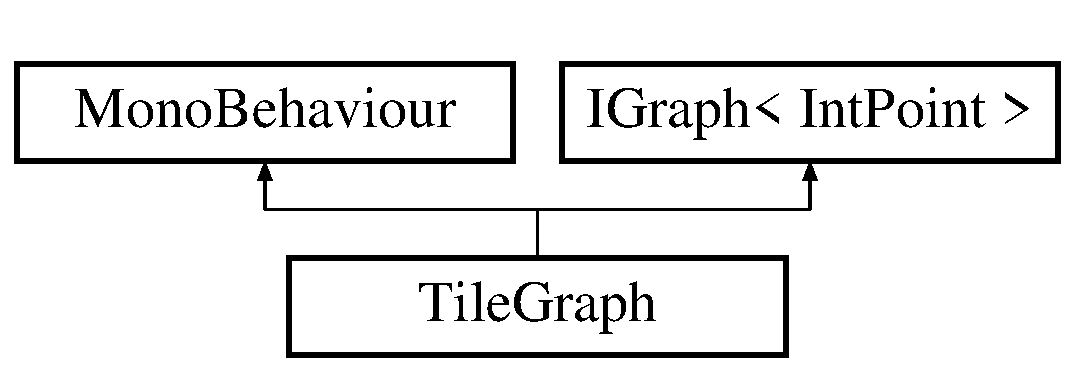
\includegraphics[height=2.000000cm]{class_tile_graph}
\end{center}
\end{figure}
\subsection*{Public Member Functions}
\begin{DoxyCompactItemize}
\item 
void \mbox{\hyperlink{class_tile_graph_a4e921f79aca67d58cad7367227fe8c06}{Awake}} ()
\item 
void \mbox{\hyperlink{class_tile_graph_a349a2602be0a8c9473aed6103955a2a6}{Init}} ()
\item 
void \mbox{\hyperlink{class_tile_graph_a839b7d0deee777d52006ad5678170694}{Init\+Height\+Field}} ()
\item 
\mbox{\hyperlink{struct_int_point}{Int\+Point}} \mbox{\hyperlink{class_tile_graph_a470894695f1deb2d9c127a1e50d0b859}{World\+To\+Tile}} (Vector2 world\+Position)
\item 
\mbox{\hyperlink{struct_int_point}{Int\+Point}} \mbox{\hyperlink{class_tile_graph_a121a3327fefcf7009e2dc3c5d1c9d310}{World\+To\+Tile}} (Vector3 world\+Position)
\item 
Vector3 \mbox{\hyperlink{class_tile_graph_ae13070f1638b7409ad1d63b5551bc3fa}{Tile\+To\+World}} (\mbox{\hyperlink{struct_int_point}{Int\+Point}} tile\+Position)
\item 
Vector3 \mbox{\hyperlink{class_tile_graph_a23609e10dfa34c3b498c3c0a35548e0f}{World\+To\+Tile\+Center}} (Vector3 world\+Position)
\item 
void \mbox{\hyperlink{class_tile_graph_a36cabbaca38766f02b95a82ee0967ebc}{Get\+Connections}} (\mbox{\hyperlink{struct_int_point}{Int\+Point}} from\+Node, out List$<$ \mbox{\hyperlink{interface_i_connection}{I\+Connection}}$<$ \mbox{\hyperlink{struct_int_point}{Int\+Point}} $>$$>$ connections)
\begin{DoxyCompactList}\small\item\em Fills connections with node connections that can be reached from from\+Node \end{DoxyCompactList}\item 
bool \mbox{\hyperlink{class_tile_graph_a9213b3332566a8e720dd28a05376001c}{Is\+Tile\+Blocked}} (\mbox{\hyperlink{struct_int_point}{Int\+Point}} tile\+Coords)
\end{DoxyCompactItemize}
\subsection*{Public Attributes}
\begin{DoxyCompactItemize}
\item 
float \mbox{\hyperlink{class_tile_graph_ae6728f48acf48baa4400f8829cc29bc3}{tile\+Size}} = 1.\+0f
\item 
Vector3 \mbox{\hyperlink{class_tile_graph_a2d996c82ced0508bb04cbdf1a45ba144}{graph\+Size}} = new Vector3(40, 1, 40)
\item 
string \mbox{[}$\,$\mbox{]} \mbox{\hyperlink{class_tile_graph_a882d4a8adc35cb6a66f4d29d63dcb0c0}{blocking}} = new string\mbox{[}1\mbox{]}
\item 
float \mbox{[},\mbox{]} \mbox{\hyperlink{class_tile_graph_a5e585742f9ecd6ce5e3a0abb55a9f89b}{height\+Values}}
\item 
Terrain \mbox{\hyperlink{class_tile_graph_a064f51b86f086091ec4b9fff14c554e2}{terrain}}
\end{DoxyCompactItemize}


\subsection{Member Function Documentation}
\mbox{\Hypertarget{class_tile_graph_a4e921f79aca67d58cad7367227fe8c06}\label{class_tile_graph_a4e921f79aca67d58cad7367227fe8c06}} 
\index{Tile\+Graph@{Tile\+Graph}!Awake@{Awake}}
\index{Awake@{Awake}!Tile\+Graph@{Tile\+Graph}}
\subsubsection{\texorpdfstring{Awake()}{Awake()}}
{\footnotesize\ttfamily void Tile\+Graph.\+Awake (\begin{DoxyParamCaption}{ }\end{DoxyParamCaption})}

\mbox{\Hypertarget{class_tile_graph_a36cabbaca38766f02b95a82ee0967ebc}\label{class_tile_graph_a36cabbaca38766f02b95a82ee0967ebc}} 
\index{Tile\+Graph@{Tile\+Graph}!Get\+Connections@{Get\+Connections}}
\index{Get\+Connections@{Get\+Connections}!Tile\+Graph@{Tile\+Graph}}
\subsubsection{\texorpdfstring{Get\+Connections()}{GetConnections()}}
{\footnotesize\ttfamily void Tile\+Graph.\+Get\+Connections (\begin{DoxyParamCaption}\item[{\mbox{\hyperlink{struct_int_point}{Int\+Point}}}]{from\+Node,  }\item[{out List$<$ \mbox{\hyperlink{interface_i_connection}{I\+Connection}}$<$ \mbox{\hyperlink{struct_int_point}{Int\+Point}} $>$$>$}]{connections }\end{DoxyParamCaption})}



Fills connections with node connections that can be reached from from\+Node 


\begin{DoxyParams}{Parameters}
{\em from\+Node} & The tile coordinates of the node to find connections for.\\
\hline
{\em connections} & The resulting set of connections\\
\hline
\end{DoxyParams}
\mbox{\Hypertarget{class_tile_graph_a349a2602be0a8c9473aed6103955a2a6}\label{class_tile_graph_a349a2602be0a8c9473aed6103955a2a6}} 
\index{Tile\+Graph@{Tile\+Graph}!Init@{Init}}
\index{Init@{Init}!Tile\+Graph@{Tile\+Graph}}
\subsubsection{\texorpdfstring{Init()}{Init()}}
{\footnotesize\ttfamily void Tile\+Graph.\+Init (\begin{DoxyParamCaption}{ }\end{DoxyParamCaption})}

\mbox{\Hypertarget{class_tile_graph_a839b7d0deee777d52006ad5678170694}\label{class_tile_graph_a839b7d0deee777d52006ad5678170694}} 
\index{Tile\+Graph@{Tile\+Graph}!Init\+Height\+Field@{Init\+Height\+Field}}
\index{Init\+Height\+Field@{Init\+Height\+Field}!Tile\+Graph@{Tile\+Graph}}
\subsubsection{\texorpdfstring{Init\+Height\+Field()}{InitHeightField()}}
{\footnotesize\ttfamily void Tile\+Graph.\+Init\+Height\+Field (\begin{DoxyParamCaption}{ }\end{DoxyParamCaption})}

\mbox{\Hypertarget{class_tile_graph_a9213b3332566a8e720dd28a05376001c}\label{class_tile_graph_a9213b3332566a8e720dd28a05376001c}} 
\index{Tile\+Graph@{Tile\+Graph}!Is\+Tile\+Blocked@{Is\+Tile\+Blocked}}
\index{Is\+Tile\+Blocked@{Is\+Tile\+Blocked}!Tile\+Graph@{Tile\+Graph}}
\subsubsection{\texorpdfstring{Is\+Tile\+Blocked()}{IsTileBlocked()}}
{\footnotesize\ttfamily bool Tile\+Graph.\+Is\+Tile\+Blocked (\begin{DoxyParamCaption}\item[{\mbox{\hyperlink{struct_int_point}{Int\+Point}}}]{tile\+Coords }\end{DoxyParamCaption})}

\mbox{\Hypertarget{class_tile_graph_ae13070f1638b7409ad1d63b5551bc3fa}\label{class_tile_graph_ae13070f1638b7409ad1d63b5551bc3fa}} 
\index{Tile\+Graph@{Tile\+Graph}!Tile\+To\+World@{Tile\+To\+World}}
\index{Tile\+To\+World@{Tile\+To\+World}!Tile\+Graph@{Tile\+Graph}}
\subsubsection{\texorpdfstring{Tile\+To\+World()}{TileToWorld()}}
{\footnotesize\ttfamily Vector3 Tile\+Graph.\+Tile\+To\+World (\begin{DoxyParamCaption}\item[{\mbox{\hyperlink{struct_int_point}{Int\+Point}}}]{tile\+Position }\end{DoxyParamCaption})}

\mbox{\Hypertarget{class_tile_graph_a470894695f1deb2d9c127a1e50d0b859}\label{class_tile_graph_a470894695f1deb2d9c127a1e50d0b859}} 
\index{Tile\+Graph@{Tile\+Graph}!World\+To\+Tile@{World\+To\+Tile}}
\index{World\+To\+Tile@{World\+To\+Tile}!Tile\+Graph@{Tile\+Graph}}
\subsubsection{\texorpdfstring{World\+To\+Tile()}{WorldToTile()}\hspace{0.1cm}{\footnotesize\ttfamily [1/2]}}
{\footnotesize\ttfamily \mbox{\hyperlink{struct_int_point}{Int\+Point}} Tile\+Graph.\+World\+To\+Tile (\begin{DoxyParamCaption}\item[{Vector2}]{world\+Position }\end{DoxyParamCaption})}

\mbox{\Hypertarget{class_tile_graph_a121a3327fefcf7009e2dc3c5d1c9d310}\label{class_tile_graph_a121a3327fefcf7009e2dc3c5d1c9d310}} 
\index{Tile\+Graph@{Tile\+Graph}!World\+To\+Tile@{World\+To\+Tile}}
\index{World\+To\+Tile@{World\+To\+Tile}!Tile\+Graph@{Tile\+Graph}}
\subsubsection{\texorpdfstring{World\+To\+Tile()}{WorldToTile()}\hspace{0.1cm}{\footnotesize\ttfamily [2/2]}}
{\footnotesize\ttfamily \mbox{\hyperlink{struct_int_point}{Int\+Point}} Tile\+Graph.\+World\+To\+Tile (\begin{DoxyParamCaption}\item[{Vector3}]{world\+Position }\end{DoxyParamCaption})}

\mbox{\Hypertarget{class_tile_graph_a23609e10dfa34c3b498c3c0a35548e0f}\label{class_tile_graph_a23609e10dfa34c3b498c3c0a35548e0f}} 
\index{Tile\+Graph@{Tile\+Graph}!World\+To\+Tile\+Center@{World\+To\+Tile\+Center}}
\index{World\+To\+Tile\+Center@{World\+To\+Tile\+Center}!Tile\+Graph@{Tile\+Graph}}
\subsubsection{\texorpdfstring{World\+To\+Tile\+Center()}{WorldToTileCenter()}}
{\footnotesize\ttfamily Vector3 Tile\+Graph.\+World\+To\+Tile\+Center (\begin{DoxyParamCaption}\item[{Vector3}]{world\+Position }\end{DoxyParamCaption})}



\subsection{Member Data Documentation}
\mbox{\Hypertarget{class_tile_graph_a882d4a8adc35cb6a66f4d29d63dcb0c0}\label{class_tile_graph_a882d4a8adc35cb6a66f4d29d63dcb0c0}} 
\index{Tile\+Graph@{Tile\+Graph}!blocking@{blocking}}
\index{blocking@{blocking}!Tile\+Graph@{Tile\+Graph}}
\subsubsection{\texorpdfstring{blocking}{blocking}}
{\footnotesize\ttfamily string \mbox{[}$\,$\mbox{]} Tile\+Graph.\+blocking = new string\mbox{[}1\mbox{]}}

\mbox{\Hypertarget{class_tile_graph_a2d996c82ced0508bb04cbdf1a45ba144}\label{class_tile_graph_a2d996c82ced0508bb04cbdf1a45ba144}} 
\index{Tile\+Graph@{Tile\+Graph}!graph\+Size@{graph\+Size}}
\index{graph\+Size@{graph\+Size}!Tile\+Graph@{Tile\+Graph}}
\subsubsection{\texorpdfstring{graph\+Size}{graphSize}}
{\footnotesize\ttfamily Vector3 Tile\+Graph.\+graph\+Size = new Vector3(40, 1, 40)}

\mbox{\Hypertarget{class_tile_graph_a5e585742f9ecd6ce5e3a0abb55a9f89b}\label{class_tile_graph_a5e585742f9ecd6ce5e3a0abb55a9f89b}} 
\index{Tile\+Graph@{Tile\+Graph}!height\+Values@{height\+Values}}
\index{height\+Values@{height\+Values}!Tile\+Graph@{Tile\+Graph}}
\subsubsection{\texorpdfstring{height\+Values}{heightValues}}
{\footnotesize\ttfamily float \mbox{[},\mbox{]} Tile\+Graph.\+height\+Values}

\mbox{\Hypertarget{class_tile_graph_a064f51b86f086091ec4b9fff14c554e2}\label{class_tile_graph_a064f51b86f086091ec4b9fff14c554e2}} 
\index{Tile\+Graph@{Tile\+Graph}!terrain@{terrain}}
\index{terrain@{terrain}!Tile\+Graph@{Tile\+Graph}}
\subsubsection{\texorpdfstring{terrain}{terrain}}
{\footnotesize\ttfamily Terrain Tile\+Graph.\+terrain}

\mbox{\Hypertarget{class_tile_graph_ae6728f48acf48baa4400f8829cc29bc3}\label{class_tile_graph_ae6728f48acf48baa4400f8829cc29bc3}} 
\index{Tile\+Graph@{Tile\+Graph}!tile\+Size@{tile\+Size}}
\index{tile\+Size@{tile\+Size}!Tile\+Graph@{Tile\+Graph}}
\subsubsection{\texorpdfstring{tile\+Size}{tileSize}}
{\footnotesize\ttfamily float Tile\+Graph.\+tile\+Size = 1.\+0f}



The documentation for this class was generated from the following file\+:\begin{DoxyCompactItemize}
\item 
/\+Users/sabienambrose/\+Documents/\+Coding/\+Unity\+Mechanical\+Turk/\+Mechanical\+Turk/\+Assets/\+Scripts/\+Util/\+Containers/\+Graphs/\+Tile\+Graphs/\mbox{\hyperlink{_tile_graph_8cs}{Tile\+Graph.\+cs}}\end{DoxyCompactItemize}

\hypertarget{struct_tile_record}{}\section{Tile\+Record Struct Reference}
\label{struct_tile_record}\index{Tile\+Record@{Tile\+Record}}
\subsection*{Public Attributes}
\begin{DoxyCompactItemize}
\item 
\mbox{\hyperlink{interface_i_connection}{I\+Connection}}$<$ \mbox{\hyperlink{struct_int_point}{Int\+Point}} $>$ \mbox{\hyperlink{struct_tile_record_acf607b02b02de7d586a00a75f341fe5e}{edge}}
\item 
float \mbox{\hyperlink{struct_tile_record_ab47bc9e2be8dc1b0a165147d2fc11d2f}{cost\+So\+Far}}
\item 
float \mbox{\hyperlink{struct_tile_record_ab2f27c5059450f78975ed349cd671b70}{estimated\+Total\+Cost}}
\item 
\mbox{\hyperlink{_graph_types_8cs_aeaefcb909e173fc6cbac62eca33b14f9}{Node\+Category}} \mbox{\hyperlink{struct_tile_record_ab64ecbc183f80275df4199c6215224bd}{category}}
\end{DoxyCompactItemize}


\subsection{Member Data Documentation}
\mbox{\Hypertarget{struct_tile_record_ab64ecbc183f80275df4199c6215224bd}\label{struct_tile_record_ab64ecbc183f80275df4199c6215224bd}} 
\index{Tile\+Record@{Tile\+Record}!category@{category}}
\index{category@{category}!Tile\+Record@{Tile\+Record}}
\subsubsection{\texorpdfstring{category}{category}}
{\footnotesize\ttfamily \mbox{\hyperlink{_graph_types_8cs_aeaefcb909e173fc6cbac62eca33b14f9}{Node\+Category}} Tile\+Record.\+category}

\mbox{\Hypertarget{struct_tile_record_ab47bc9e2be8dc1b0a165147d2fc11d2f}\label{struct_tile_record_ab47bc9e2be8dc1b0a165147d2fc11d2f}} 
\index{Tile\+Record@{Tile\+Record}!cost\+So\+Far@{cost\+So\+Far}}
\index{cost\+So\+Far@{cost\+So\+Far}!Tile\+Record@{Tile\+Record}}
\subsubsection{\texorpdfstring{cost\+So\+Far}{costSoFar}}
{\footnotesize\ttfamily float Tile\+Record.\+cost\+So\+Far}

\mbox{\Hypertarget{struct_tile_record_acf607b02b02de7d586a00a75f341fe5e}\label{struct_tile_record_acf607b02b02de7d586a00a75f341fe5e}} 
\index{Tile\+Record@{Tile\+Record}!edge@{edge}}
\index{edge@{edge}!Tile\+Record@{Tile\+Record}}
\subsubsection{\texorpdfstring{edge}{edge}}
{\footnotesize\ttfamily \mbox{\hyperlink{interface_i_connection}{I\+Connection}}$<$\mbox{\hyperlink{struct_int_point}{Int\+Point}}$>$ Tile\+Record.\+edge}

\mbox{\Hypertarget{struct_tile_record_ab2f27c5059450f78975ed349cd671b70}\label{struct_tile_record_ab2f27c5059450f78975ed349cd671b70}} 
\index{Tile\+Record@{Tile\+Record}!estimated\+Total\+Cost@{estimated\+Total\+Cost}}
\index{estimated\+Total\+Cost@{estimated\+Total\+Cost}!Tile\+Record@{Tile\+Record}}
\subsubsection{\texorpdfstring{estimated\+Total\+Cost}{estimatedTotalCost}}
{\footnotesize\ttfamily float Tile\+Record.\+estimated\+Total\+Cost}



The documentation for this struct was generated from the following file\+:\begin{DoxyCompactItemize}
\item 
/\+Users/sabienambrose/\+Documents/\+Coding/\+Unity\+Mechanical\+Turk/\+Mechanical\+Turk/\+Assets/\+Scripts/\+Util/\+Containers/\+Graphs/\mbox{\hyperlink{_graph_types_8cs}{Graph\+Types.\+cs}}\end{DoxyCompactItemize}

\hypertarget{class_tile_world}{}\section{Tile\+World Class Reference}
\label{class_tile_world}\index{Tile\+World@{Tile\+World}}
Inheritance diagram for Tile\+World\+:\begin{figure}[H]
\begin{center}
\leavevmode
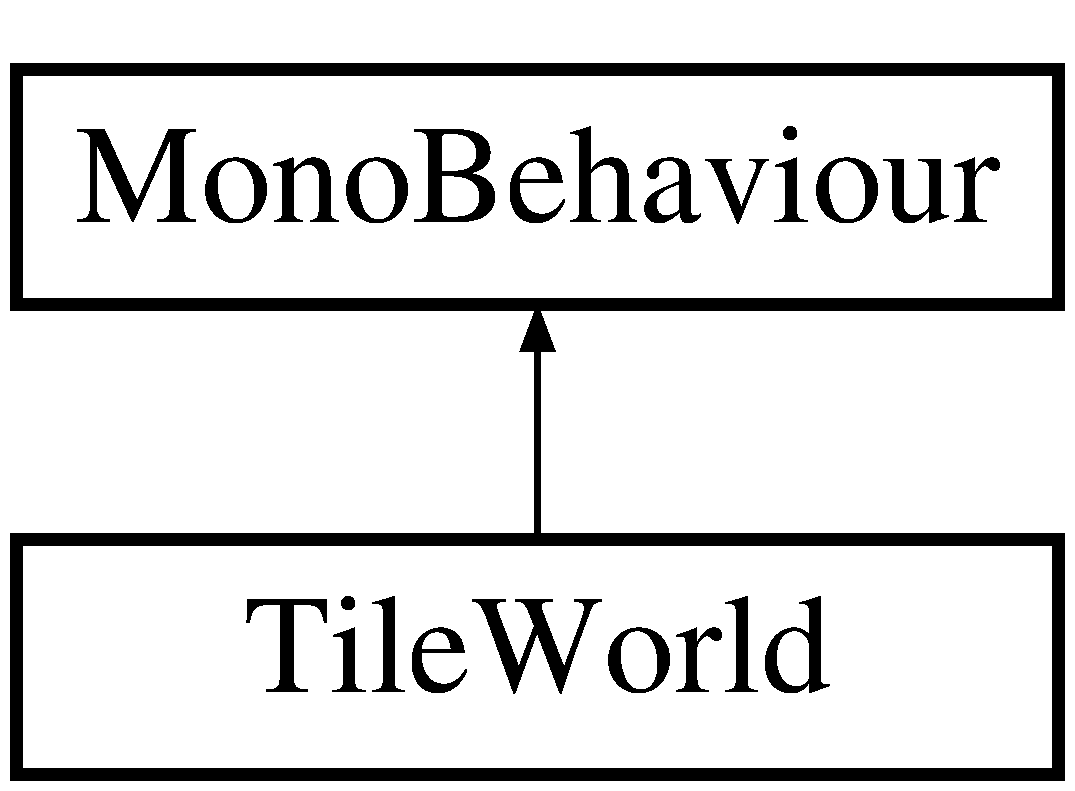
\includegraphics[height=2.000000cm]{class_tile_world}
\end{center}
\end{figure}
\subsection*{Public Member Functions}
\begin{DoxyCompactItemize}
\item 
void \mbox{\hyperlink{class_tile_world_ac42e3485b2e38601dd47dcb12b5af1d8}{Awake}} ()
\item 
void \mbox{\hyperlink{class_tile_world_ad236fe1c3f6a9f3bd6f1811962e8d849}{Init}} ()
\item 
void \mbox{\hyperlink{class_tile_world_a1888b1fe49ca8b7a58b982cb25ddd7f0}{Clear\+Nodes}} ()
\item 
void \mbox{\hyperlink{class_tile_world_a377f2b3e756ec6d9eee11fad9fb3688f}{Set\+Node\+Category}} (\mbox{\hyperlink{struct_int_point}{Int\+Point}} node, \mbox{\hyperlink{_graph_types_8cs_aeaefcb909e173fc6cbac62eca33b14f9}{Node\+Category}} category)
\item 
\mbox{\hyperlink{struct_tile_record}{Tile\+Record}} \mbox{\hyperlink{class_tile_world_aeeb99a43018c8bcbc49054e248429291}{Get\+Record\+At}} (\mbox{\hyperlink{struct_int_point}{Int\+Point}} node)
\item 
void \mbox{\hyperlink{class_tile_world_ad06ad6b7b31c633d59cd494747070d9b}{On\+Draw\+Gizmos}} ()
\end{DoxyCompactItemize}
\subsection*{Public Attributes}
\begin{DoxyCompactItemize}
\item 
\mbox{\hyperlink{class_tile_graph}{Tile\+Graph}} \mbox{\hyperlink{class_tile_world_af281625545d4b1aaeaf5053a62b1d519}{tile\+Graph}}
\item 
bool \mbox{\hyperlink{class_tile_world_af3b21e656a6ba363f41fe128a7e02be2}{draw\+Records}} = false
\item 
bool \mbox{\hyperlink{class_tile_world_abcf86ec3be82b6a58b64f7dad278b1e0}{draw\+Blocking}} = false
\item 
\mbox{\hyperlink{struct_tile_record}{Tile\+Record}} \mbox{[},\mbox{]} \mbox{\hyperlink{class_tile_world_a8f7c8f36d84d1bd4086078e690a08ce3}{node\+Array}}
\end{DoxyCompactItemize}


\subsection{Member Function Documentation}
\mbox{\Hypertarget{class_tile_world_ac42e3485b2e38601dd47dcb12b5af1d8}\label{class_tile_world_ac42e3485b2e38601dd47dcb12b5af1d8}} 
\index{Tile\+World@{Tile\+World}!Awake@{Awake}}
\index{Awake@{Awake}!Tile\+World@{Tile\+World}}
\subsubsection{\texorpdfstring{Awake()}{Awake()}}
{\footnotesize\ttfamily void Tile\+World.\+Awake (\begin{DoxyParamCaption}{ }\end{DoxyParamCaption})}

\mbox{\Hypertarget{class_tile_world_a1888b1fe49ca8b7a58b982cb25ddd7f0}\label{class_tile_world_a1888b1fe49ca8b7a58b982cb25ddd7f0}} 
\index{Tile\+World@{Tile\+World}!Clear\+Nodes@{Clear\+Nodes}}
\index{Clear\+Nodes@{Clear\+Nodes}!Tile\+World@{Tile\+World}}
\subsubsection{\texorpdfstring{Clear\+Nodes()}{ClearNodes()}}
{\footnotesize\ttfamily void Tile\+World.\+Clear\+Nodes (\begin{DoxyParamCaption}{ }\end{DoxyParamCaption})}

\mbox{\Hypertarget{class_tile_world_aeeb99a43018c8bcbc49054e248429291}\label{class_tile_world_aeeb99a43018c8bcbc49054e248429291}} 
\index{Tile\+World@{Tile\+World}!Get\+Record\+At@{Get\+Record\+At}}
\index{Get\+Record\+At@{Get\+Record\+At}!Tile\+World@{Tile\+World}}
\subsubsection{\texorpdfstring{Get\+Record\+At()}{GetRecordAt()}}
{\footnotesize\ttfamily \mbox{\hyperlink{struct_tile_record}{Tile\+Record}} Tile\+World.\+Get\+Record\+At (\begin{DoxyParamCaption}\item[{\mbox{\hyperlink{struct_int_point}{Int\+Point}}}]{node }\end{DoxyParamCaption})}

\mbox{\Hypertarget{class_tile_world_ad236fe1c3f6a9f3bd6f1811962e8d849}\label{class_tile_world_ad236fe1c3f6a9f3bd6f1811962e8d849}} 
\index{Tile\+World@{Tile\+World}!Init@{Init}}
\index{Init@{Init}!Tile\+World@{Tile\+World}}
\subsubsection{\texorpdfstring{Init()}{Init()}}
{\footnotesize\ttfamily void Tile\+World.\+Init (\begin{DoxyParamCaption}{ }\end{DoxyParamCaption})}

\mbox{\Hypertarget{class_tile_world_ad06ad6b7b31c633d59cd494747070d9b}\label{class_tile_world_ad06ad6b7b31c633d59cd494747070d9b}} 
\index{Tile\+World@{Tile\+World}!On\+Draw\+Gizmos@{On\+Draw\+Gizmos}}
\index{On\+Draw\+Gizmos@{On\+Draw\+Gizmos}!Tile\+World@{Tile\+World}}
\subsubsection{\texorpdfstring{On\+Draw\+Gizmos()}{OnDrawGizmos()}}
{\footnotesize\ttfamily void Tile\+World.\+On\+Draw\+Gizmos (\begin{DoxyParamCaption}{ }\end{DoxyParamCaption})}

\mbox{\Hypertarget{class_tile_world_a377f2b3e756ec6d9eee11fad9fb3688f}\label{class_tile_world_a377f2b3e756ec6d9eee11fad9fb3688f}} 
\index{Tile\+World@{Tile\+World}!Set\+Node\+Category@{Set\+Node\+Category}}
\index{Set\+Node\+Category@{Set\+Node\+Category}!Tile\+World@{Tile\+World}}
\subsubsection{\texorpdfstring{Set\+Node\+Category()}{SetNodeCategory()}}
{\footnotesize\ttfamily void Tile\+World.\+Set\+Node\+Category (\begin{DoxyParamCaption}\item[{\mbox{\hyperlink{struct_int_point}{Int\+Point}}}]{node,  }\item[{\mbox{\hyperlink{_graph_types_8cs_aeaefcb909e173fc6cbac62eca33b14f9}{Node\+Category}}}]{category }\end{DoxyParamCaption})}



\subsection{Member Data Documentation}
\mbox{\Hypertarget{class_tile_world_abcf86ec3be82b6a58b64f7dad278b1e0}\label{class_tile_world_abcf86ec3be82b6a58b64f7dad278b1e0}} 
\index{Tile\+World@{Tile\+World}!draw\+Blocking@{draw\+Blocking}}
\index{draw\+Blocking@{draw\+Blocking}!Tile\+World@{Tile\+World}}
\subsubsection{\texorpdfstring{draw\+Blocking}{drawBlocking}}
{\footnotesize\ttfamily bool Tile\+World.\+draw\+Blocking = false}

\mbox{\Hypertarget{class_tile_world_af3b21e656a6ba363f41fe128a7e02be2}\label{class_tile_world_af3b21e656a6ba363f41fe128a7e02be2}} 
\index{Tile\+World@{Tile\+World}!draw\+Records@{draw\+Records}}
\index{draw\+Records@{draw\+Records}!Tile\+World@{Tile\+World}}
\subsubsection{\texorpdfstring{draw\+Records}{drawRecords}}
{\footnotesize\ttfamily bool Tile\+World.\+draw\+Records = false}

\mbox{\Hypertarget{class_tile_world_a8f7c8f36d84d1bd4086078e690a08ce3}\label{class_tile_world_a8f7c8f36d84d1bd4086078e690a08ce3}} 
\index{Tile\+World@{Tile\+World}!node\+Array@{node\+Array}}
\index{node\+Array@{node\+Array}!Tile\+World@{Tile\+World}}
\subsubsection{\texorpdfstring{node\+Array}{nodeArray}}
{\footnotesize\ttfamily \mbox{\hyperlink{struct_tile_record}{Tile\+Record}} \mbox{[},\mbox{]} Tile\+World.\+node\+Array}

\mbox{\Hypertarget{class_tile_world_af281625545d4b1aaeaf5053a62b1d519}\label{class_tile_world_af281625545d4b1aaeaf5053a62b1d519}} 
\index{Tile\+World@{Tile\+World}!tile\+Graph@{tile\+Graph}}
\index{tile\+Graph@{tile\+Graph}!Tile\+World@{Tile\+World}}
\subsubsection{\texorpdfstring{tile\+Graph}{tileGraph}}
{\footnotesize\ttfamily \mbox{\hyperlink{class_tile_graph}{Tile\+Graph}} Tile\+World.\+tile\+Graph}



The documentation for this class was generated from the following file\+:\begin{DoxyCompactItemize}
\item 
/\+Users/sabienambrose/\+Documents/\+Coding/\+Unity\+Mechanical\+Turk/\+Mechanical\+Turk/\+Assets/\+Scripts/\+Util/\+Containers/\+Graphs/\+Tile\+Graphs/\mbox{\hyperlink{_tile_world_8cs}{Tile\+World.\+cs}}\end{DoxyCompactItemize}

\hypertarget{class_utility_system_1_1_utility_properties}{}\section{Utility\+System.\+Utility\+Properties Class Reference}
\label{class_utility_system_1_1_utility_properties}\index{Utility\+System.\+Utility\+Properties@{Utility\+System.\+Utility\+Properties}}
Inheritance diagram for Utility\+System.\+Utility\+Properties\+:\begin{figure}[H]
\begin{center}
\leavevmode
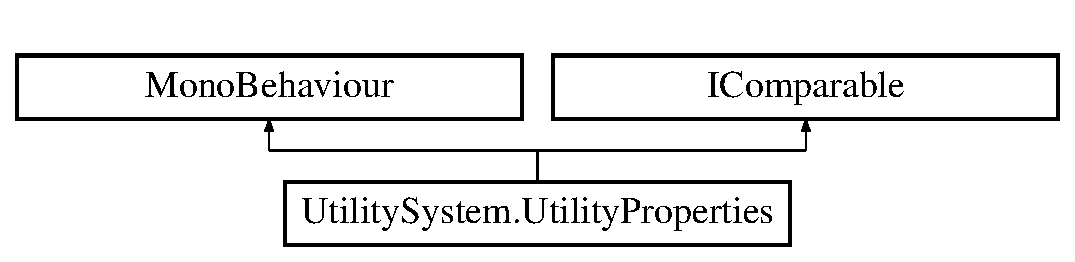
\includegraphics[height=2.000000cm]{class_utility_system_1_1_utility_properties}
\end{center}
\end{figure}
\subsection*{Public Member Functions}
\begin{DoxyCompactItemize}
\item 
void \mbox{\hyperlink{class_utility_system_1_1_utility_properties_a9919d860fe70280710b938d2946a7d0a}{Start}} ()
\item 
void \mbox{\hyperlink{class_utility_system_1_1_utility_properties_ac37ea8be2246d96257bf94ff9b22ec98}{On\+Validate}} ()
\item 
virtual float \mbox{\hyperlink{class_utility_system_1_1_utility_properties_a8a6f5a57649bcd38f2e880a4afcd719d}{Get\+Utility}} ()
\item 
int \mbox{\hyperlink{class_utility_system_1_1_utility_properties_a0b6edfa9fe4c35ca1f2b2ce91b27b379}{Compare\+To}} (object obj)
\item 
int \mbox{\hyperlink{class_utility_system_1_1_utility_properties_a152bc86d4852fe36a2bee38e478b44ad}{Compare\+To}} (\mbox{\hyperlink{class_utility_system_1_1_utility_properties}{Utility\+Properties}} other)
\end{DoxyCompactItemize}
\subsection*{Public Attributes}
\begin{DoxyCompactItemize}
\item 
float \mbox{[}$\,$\mbox{]} \mbox{\hyperlink{class_utility_system_1_1_utility_properties_abb078a8e18ca126eec98a9cc1dd3f703}{weights}}
\end{DoxyCompactItemize}


\subsection{Member Function Documentation}
\mbox{\Hypertarget{class_utility_system_1_1_utility_properties_a0b6edfa9fe4c35ca1f2b2ce91b27b379}\label{class_utility_system_1_1_utility_properties_a0b6edfa9fe4c35ca1f2b2ce91b27b379}} 
\index{Utility\+System\+::\+Utility\+Properties@{Utility\+System\+::\+Utility\+Properties}!Compare\+To@{Compare\+To}}
\index{Compare\+To@{Compare\+To}!Utility\+System\+::\+Utility\+Properties@{Utility\+System\+::\+Utility\+Properties}}
\subsubsection{\texorpdfstring{Compare\+To()}{CompareTo()}\hspace{0.1cm}{\footnotesize\ttfamily [1/2]}}
{\footnotesize\ttfamily int Utility\+System.\+Utility\+Properties.\+Compare\+To (\begin{DoxyParamCaption}\item[{object}]{obj }\end{DoxyParamCaption})}

\mbox{\Hypertarget{class_utility_system_1_1_utility_properties_a152bc86d4852fe36a2bee38e478b44ad}\label{class_utility_system_1_1_utility_properties_a152bc86d4852fe36a2bee38e478b44ad}} 
\index{Utility\+System\+::\+Utility\+Properties@{Utility\+System\+::\+Utility\+Properties}!Compare\+To@{Compare\+To}}
\index{Compare\+To@{Compare\+To}!Utility\+System\+::\+Utility\+Properties@{Utility\+System\+::\+Utility\+Properties}}
\subsubsection{\texorpdfstring{Compare\+To()}{CompareTo()}\hspace{0.1cm}{\footnotesize\ttfamily [2/2]}}
{\footnotesize\ttfamily int Utility\+System.\+Utility\+Properties.\+Compare\+To (\begin{DoxyParamCaption}\item[{\mbox{\hyperlink{class_utility_system_1_1_utility_properties}{Utility\+Properties}}}]{other }\end{DoxyParamCaption})}

\mbox{\Hypertarget{class_utility_system_1_1_utility_properties_a8a6f5a57649bcd38f2e880a4afcd719d}\label{class_utility_system_1_1_utility_properties_a8a6f5a57649bcd38f2e880a4afcd719d}} 
\index{Utility\+System\+::\+Utility\+Properties@{Utility\+System\+::\+Utility\+Properties}!Get\+Utility@{Get\+Utility}}
\index{Get\+Utility@{Get\+Utility}!Utility\+System\+::\+Utility\+Properties@{Utility\+System\+::\+Utility\+Properties}}
\subsubsection{\texorpdfstring{Get\+Utility()}{GetUtility()}}
{\footnotesize\ttfamily virtual float Utility\+System.\+Utility\+Properties.\+Get\+Utility (\begin{DoxyParamCaption}{ }\end{DoxyParamCaption})\hspace{0.3cm}{\ttfamily [virtual]}}

\mbox{\Hypertarget{class_utility_system_1_1_utility_properties_ac37ea8be2246d96257bf94ff9b22ec98}\label{class_utility_system_1_1_utility_properties_ac37ea8be2246d96257bf94ff9b22ec98}} 
\index{Utility\+System\+::\+Utility\+Properties@{Utility\+System\+::\+Utility\+Properties}!On\+Validate@{On\+Validate}}
\index{On\+Validate@{On\+Validate}!Utility\+System\+::\+Utility\+Properties@{Utility\+System\+::\+Utility\+Properties}}
\subsubsection{\texorpdfstring{On\+Validate()}{OnValidate()}}
{\footnotesize\ttfamily void Utility\+System.\+Utility\+Properties.\+On\+Validate (\begin{DoxyParamCaption}{ }\end{DoxyParamCaption})}

\mbox{\Hypertarget{class_utility_system_1_1_utility_properties_a9919d860fe70280710b938d2946a7d0a}\label{class_utility_system_1_1_utility_properties_a9919d860fe70280710b938d2946a7d0a}} 
\index{Utility\+System\+::\+Utility\+Properties@{Utility\+System\+::\+Utility\+Properties}!Start@{Start}}
\index{Start@{Start}!Utility\+System\+::\+Utility\+Properties@{Utility\+System\+::\+Utility\+Properties}}
\subsubsection{\texorpdfstring{Start()}{Start()}}
{\footnotesize\ttfamily void Utility\+System.\+Utility\+Properties.\+Start (\begin{DoxyParamCaption}{ }\end{DoxyParamCaption})}



\subsection{Member Data Documentation}
\mbox{\Hypertarget{class_utility_system_1_1_utility_properties_abb078a8e18ca126eec98a9cc1dd3f703}\label{class_utility_system_1_1_utility_properties_abb078a8e18ca126eec98a9cc1dd3f703}} 
\index{Utility\+System\+::\+Utility\+Properties@{Utility\+System\+::\+Utility\+Properties}!weights@{weights}}
\index{weights@{weights}!Utility\+System\+::\+Utility\+Properties@{Utility\+System\+::\+Utility\+Properties}}
\subsubsection{\texorpdfstring{weights}{weights}}
{\footnotesize\ttfamily float \mbox{[}$\,$\mbox{]} Utility\+System.\+Utility\+Properties.\+weights}



The documentation for this class was generated from the following file\+:\begin{DoxyCompactItemize}
\item 
/\+Users/sabienambrose/\+Documents/\+Coding/\+Unity\+Mechanical\+Turk/\+Mechanical\+Turk/\+Assets/\+Scripts/\+Pathfinding/\+Utility/\mbox{\hyperlink{_utility_properties_8cs}{Utility\+Properties.\+cs}}\end{DoxyCompactItemize}

\hypertarget{class_world_gen_context}{}\section{World\+Gen\+Context Class Reference}
\label{class_world_gen_context}\index{World\+Gen\+Context@{World\+Gen\+Context}}
Inheritance diagram for World\+Gen\+Context\+:\begin{figure}[H]
\begin{center}
\leavevmode
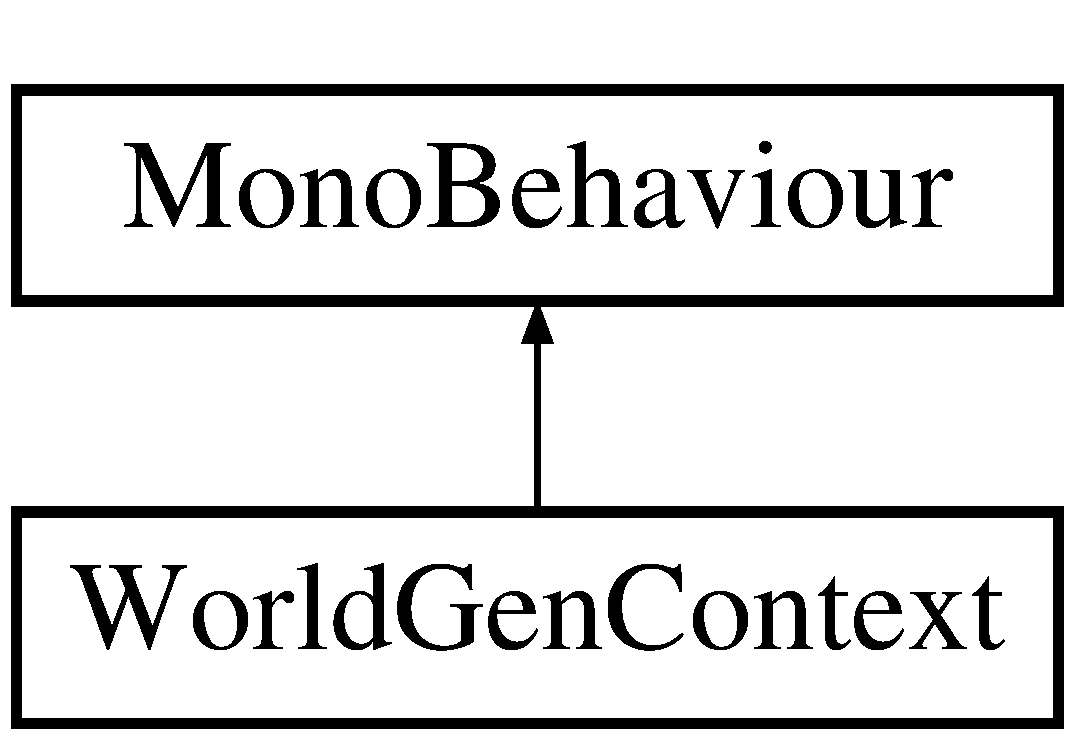
\includegraphics[height=2.000000cm]{class_world_gen_context}
\end{center}
\end{figure}


The documentation for this class was generated from the following file\+:\begin{DoxyCompactItemize}
\item 
/\+Users/sabienambrose/\+Documents/\+Coding/\+Unity\+Mechanical\+Turk/\+Mechanical\+Turk/\+Assets/\+Scripts/\+Pathfinding/\+Utility/\+Context/\mbox{\hyperlink{_world_gen_context_8cs}{World\+Gen\+Context.\+cs}}\end{DoxyCompactItemize}

\chapter{File Documentation}
\hypertarget{_city_generator_8cs}{}\section{/\+Users/sabienambrose/\+Documents/\+Coding/\+Unity\+Mechanical\+Turk/\+Mechanical\+Turk/\+Assets/\+Scripts/\+Framework/\+Generation/\+City\+Generator.cs File Reference}
\label{_city_generator_8cs}\index{/\+Users/sabienambrose/\+Documents/\+Coding/\+Unity\+Mechanical\+Turk/\+Mechanical\+Turk/\+Assets/\+Scripts/\+Framework/\+Generation/\+City\+Generator.\+cs@{/\+Users/sabienambrose/\+Documents/\+Coding/\+Unity\+Mechanical\+Turk/\+Mechanical\+Turk/\+Assets/\+Scripts/\+Framework/\+Generation/\+City\+Generator.\+cs}}
\subsection*{Classes}
\begin{DoxyCompactItemize}
\item 
class \mbox{\hyperlink{class_city_generator}{City\+Generator}}
\end{DoxyCompactItemize}

\hypertarget{_generation_algorithm_8cs}{}\section{/\+Users/sabienambrose/\+Documents/\+Coding/\+Unity\+Mechanical\+Turk/\+Mechanical\+Turk/\+Assets/\+Scripts/\+Framework/\+Generation/\+Generation\+Algorithm.cs File Reference}
\label{_generation_algorithm_8cs}\index{/\+Users/sabienambrose/\+Documents/\+Coding/\+Unity\+Mechanical\+Turk/\+Mechanical\+Turk/\+Assets/\+Scripts/\+Framework/\+Generation/\+Generation\+Algorithm.\+cs@{/\+Users/sabienambrose/\+Documents/\+Coding/\+Unity\+Mechanical\+Turk/\+Mechanical\+Turk/\+Assets/\+Scripts/\+Framework/\+Generation/\+Generation\+Algorithm.\+cs}}
\subsection*{Classes}
\begin{DoxyCompactItemize}
\item 
class \mbox{\hyperlink{class_generation_algorithm}{Generation\+Algorithm}}
\begin{DoxyCompactList}\small\item\em Wrapper for various generation algorithms that adds events. \end{DoxyCompactList}\end{DoxyCompactItemize}

\hypertarget{_generation_controller_8cs}{}\section{/\+Users/sabienambrose/\+Documents/\+Coding/\+Unity\+Mechanical\+Turk/\+Mechanical\+Turk/\+Assets/\+Scripts/\+Framework/\+Generation/\+Generation\+Controller.cs File Reference}
\label{_generation_controller_8cs}\index{/\+Users/sabienambrose/\+Documents/\+Coding/\+Unity\+Mechanical\+Turk/\+Mechanical\+Turk/\+Assets/\+Scripts/\+Framework/\+Generation/\+Generation\+Controller.\+cs@{/\+Users/sabienambrose/\+Documents/\+Coding/\+Unity\+Mechanical\+Turk/\+Mechanical\+Turk/\+Assets/\+Scripts/\+Framework/\+Generation/\+Generation\+Controller.\+cs}}
\subsection*{Classes}
\begin{DoxyCompactItemize}
\item 
class \mbox{\hyperlink{class_generation_controller}{Generation\+Controller}}
\begin{DoxyCompactList}\small\item\em Manages Random Seed, Generation Sequences. \end{DoxyCompactList}\end{DoxyCompactItemize}

\hypertarget{_generation_sequence_8cs}{}\section{/\+Users/sabienambrose/\+Documents/\+Coding/\+Unity\+Mechanical\+Turk/\+Mechanical\+Turk/\+Assets/\+Scripts/\+Framework/\+Generation/\+Generation\+Sequence.cs File Reference}
\label{_generation_sequence_8cs}\index{/\+Users/sabienambrose/\+Documents/\+Coding/\+Unity\+Mechanical\+Turk/\+Mechanical\+Turk/\+Assets/\+Scripts/\+Framework/\+Generation/\+Generation\+Sequence.\+cs@{/\+Users/sabienambrose/\+Documents/\+Coding/\+Unity\+Mechanical\+Turk/\+Mechanical\+Turk/\+Assets/\+Scripts/\+Framework/\+Generation/\+Generation\+Sequence.\+cs}}
\subsection*{Classes}
\begin{DoxyCompactItemize}
\item 
class \mbox{\hyperlink{class_generation_sequence}{Generation\+Sequence}}
\end{DoxyCompactItemize}

\hypertarget{_noise_generator_8cs}{}\section{/\+Users/sabienambrose/\+Documents/\+Coding/\+Unity\+Mechanical\+Turk/\+Mechanical\+Turk/\+Assets/\+Scripts/\+Framework/\+Generation/\+Noise\+Generator.cs File Reference}
\label{_noise_generator_8cs}\index{/\+Users/sabienambrose/\+Documents/\+Coding/\+Unity\+Mechanical\+Turk/\+Mechanical\+Turk/\+Assets/\+Scripts/\+Framework/\+Generation/\+Noise\+Generator.\+cs@{/\+Users/sabienambrose/\+Documents/\+Coding/\+Unity\+Mechanical\+Turk/\+Mechanical\+Turk/\+Assets/\+Scripts/\+Framework/\+Generation/\+Noise\+Generator.\+cs}}
\subsection*{Classes}
\begin{DoxyCompactItemize}
\item 
class \mbox{\hyperlink{class_noise_generator}{Noise\+Generator}}
\end{DoxyCompactItemize}

\hypertarget{_object_picker_8cs}{}\section{/\+Users/sabienambrose/\+Documents/\+Coding/\+Unity\+Mechanical\+Turk/\+Mechanical\+Turk/\+Assets/\+Scripts/\+Framework/\+Generation/\+Object\+Picker.cs File Reference}
\label{_object_picker_8cs}\index{/\+Users/sabienambrose/\+Documents/\+Coding/\+Unity\+Mechanical\+Turk/\+Mechanical\+Turk/\+Assets/\+Scripts/\+Framework/\+Generation/\+Object\+Picker.\+cs@{/\+Users/sabienambrose/\+Documents/\+Coding/\+Unity\+Mechanical\+Turk/\+Mechanical\+Turk/\+Assets/\+Scripts/\+Framework/\+Generation/\+Object\+Picker.\+cs}}
\subsection*{Classes}
\begin{DoxyCompactItemize}
\item 
class \mbox{\hyperlink{class_object_picker}{Object\+Picker}}
\end{DoxyCompactItemize}
\subsection*{Enumerations}
\begin{DoxyCompactItemize}
\item 
enum \mbox{\hyperlink{_object_picker_8cs_a2dcef18caa6de91171bf235b9189206d}{Selection\+Method}} \{ \mbox{\hyperlink{_object_picker_8cs_a2dcef18caa6de91171bf235b9189206da64663f4646781c9c0110838b905daa23}{Selection\+Method.\+Random}}, 
\mbox{\hyperlink{_object_picker_8cs_a2dcef18caa6de91171bf235b9189206da8d6c94f57a81f3b1499c9785061cae42}{Selection\+Method.\+Min\+Utility}}, 
\mbox{\hyperlink{_object_picker_8cs_a2dcef18caa6de91171bf235b9189206daec0eedda0a9f5b2769c2c4f472069c72}{Selection\+Method.\+Max\+Utility}}
 \}
\end{DoxyCompactItemize}


\subsection{Enumeration Type Documentation}
\mbox{\Hypertarget{_object_picker_8cs_a2dcef18caa6de91171bf235b9189206d}\label{_object_picker_8cs_a2dcef18caa6de91171bf235b9189206d}} 
\index{Object\+Picker.\+cs@{Object\+Picker.\+cs}!Selection\+Method@{Selection\+Method}}
\index{Selection\+Method@{Selection\+Method}!Object\+Picker.\+cs@{Object\+Picker.\+cs}}
\subsubsection{\texorpdfstring{Selection\+Method}{SelectionMethod}}
{\footnotesize\ttfamily enum \mbox{\hyperlink{_object_picker_8cs_a2dcef18caa6de91171bf235b9189206d}{Selection\+Method}}\hspace{0.3cm}{\ttfamily [strong]}}

\begin{DoxyEnumFields}{Enumerator}
\raisebox{\heightof{T}}[0pt][0pt]{\index{Random@{Random}!Object\+Picker.\+cs@{Object\+Picker.\+cs}}\index{Object\+Picker.\+cs@{Object\+Picker.\+cs}!Random@{Random}}}\mbox{\Hypertarget{_object_picker_8cs_a2dcef18caa6de91171bf235b9189206da64663f4646781c9c0110838b905daa23}\label{_object_picker_8cs_a2dcef18caa6de91171bf235b9189206da64663f4646781c9c0110838b905daa23}} 
Random&\\
\hline

\raisebox{\heightof{T}}[0pt][0pt]{\index{Min\+Utility@{Min\+Utility}!Object\+Picker.\+cs@{Object\+Picker.\+cs}}\index{Object\+Picker.\+cs@{Object\+Picker.\+cs}!Min\+Utility@{Min\+Utility}}}\mbox{\Hypertarget{_object_picker_8cs_a2dcef18caa6de91171bf235b9189206da8d6c94f57a81f3b1499c9785061cae42}\label{_object_picker_8cs_a2dcef18caa6de91171bf235b9189206da8d6c94f57a81f3b1499c9785061cae42}} 
Min\+Utility&\\
\hline

\raisebox{\heightof{T}}[0pt][0pt]{\index{Max\+Utility@{Max\+Utility}!Object\+Picker.\+cs@{Object\+Picker.\+cs}}\index{Object\+Picker.\+cs@{Object\+Picker.\+cs}!Max\+Utility@{Max\+Utility}}}\mbox{\Hypertarget{_object_picker_8cs_a2dcef18caa6de91171bf235b9189206daec0eedda0a9f5b2769c2c4f472069c72}\label{_object_picker_8cs_a2dcef18caa6de91171bf235b9189206daec0eedda0a9f5b2769c2c4f472069c72}} 
Max\+Utility&\\
\hline

\end{DoxyEnumFields}

\hypertarget{_point_generator_8cs}{}\section{/\+Users/sabienambrose/\+Documents/\+Coding/\+Unity\+Mechanical\+Turk/\+Mechanical\+Turk/\+Assets/\+Scripts/\+Framework/\+Generation/\+Point\+Generator.cs File Reference}
\label{_point_generator_8cs}\index{/\+Users/sabienambrose/\+Documents/\+Coding/\+Unity\+Mechanical\+Turk/\+Mechanical\+Turk/\+Assets/\+Scripts/\+Framework/\+Generation/\+Point\+Generator.\+cs@{/\+Users/sabienambrose/\+Documents/\+Coding/\+Unity\+Mechanical\+Turk/\+Mechanical\+Turk/\+Assets/\+Scripts/\+Framework/\+Generation/\+Point\+Generator.\+cs}}
\subsection*{Classes}
\begin{DoxyCompactItemize}
\item 
class \mbox{\hyperlink{class_point_generator}{Point\+Generator}}
\end{DoxyCompactItemize}

\hypertarget{_consideration_8cs}{}\section{/\+Users/sabienambrose/\+Documents/\+Coding/\+Unity\+Mechanical\+Turk/\+Mechanical\+Turk/\+Assets/\+Scripts/\+Framework/\+Utility/\+Consideration.cs File Reference}
\label{_consideration_8cs}\index{/\+Users/sabienambrose/\+Documents/\+Coding/\+Unity\+Mechanical\+Turk/\+Mechanical\+Turk/\+Assets/\+Scripts/\+Framework/\+Utility/\+Consideration.\+cs@{/\+Users/sabienambrose/\+Documents/\+Coding/\+Unity\+Mechanical\+Turk/\+Mechanical\+Turk/\+Assets/\+Scripts/\+Framework/\+Utility/\+Consideration.\+cs}}
\subsection*{Classes}
\begin{DoxyCompactItemize}
\item 
class \mbox{\hyperlink{class_utility_system_1_1_consideration}{Utility\+System.\+Consideration}}
\end{DoxyCompactItemize}
\subsection*{Namespaces}
\begin{DoxyCompactItemize}
\item 
namespace \mbox{\hyperlink{namespace_utility_system}{Utility\+System}}
\end{DoxyCompactItemize}

\hypertarget{_decision_8cs}{}\section{/\+Users/sabienambrose/\+Documents/\+Coding/\+Unity\+Mechanical\+Turk/\+Mechanical\+Turk/\+Assets/\+Scripts/\+Framework/\+Utility/\+Decision.cs File Reference}
\label{_decision_8cs}\index{/\+Users/sabienambrose/\+Documents/\+Coding/\+Unity\+Mechanical\+Turk/\+Mechanical\+Turk/\+Assets/\+Scripts/\+Framework/\+Utility/\+Decision.\+cs@{/\+Users/sabienambrose/\+Documents/\+Coding/\+Unity\+Mechanical\+Turk/\+Mechanical\+Turk/\+Assets/\+Scripts/\+Framework/\+Utility/\+Decision.\+cs}}
\subsection*{Classes}
\begin{DoxyCompactItemize}
\item 
class \mbox{\hyperlink{class_utility_system_1_1_decision}{Utility\+System.\+Decision}}
\end{DoxyCompactItemize}
\subsection*{Namespaces}
\begin{DoxyCompactItemize}
\item 
namespace \mbox{\hyperlink{namespace_utility_system}{Utility\+System}}
\end{DoxyCompactItemize}

\hypertarget{_decision_context_8cs}{}\section{/\+Users/sabienambrose/\+Documents/\+Coding/\+Unity\+Mechanical\+Turk/\+Mechanical\+Turk/\+Assets/\+Scripts/\+Framework/\+Utility/\+Decision\+Context.cs File Reference}
\label{_decision_context_8cs}\index{/\+Users/sabienambrose/\+Documents/\+Coding/\+Unity\+Mechanical\+Turk/\+Mechanical\+Turk/\+Assets/\+Scripts/\+Framework/\+Utility/\+Decision\+Context.\+cs@{/\+Users/sabienambrose/\+Documents/\+Coding/\+Unity\+Mechanical\+Turk/\+Mechanical\+Turk/\+Assets/\+Scripts/\+Framework/\+Utility/\+Decision\+Context.\+cs}}
\subsection*{Classes}
\begin{DoxyCompactItemize}
\item 
class \mbox{\hyperlink{class_utility_system_1_1_decision_context}{Utility\+System.\+Decision\+Context}}
\end{DoxyCompactItemize}
\subsection*{Namespaces}
\begin{DoxyCompactItemize}
\item 
namespace \mbox{\hyperlink{namespace_utility_system}{Utility\+System}}
\end{DoxyCompactItemize}

\hypertarget{_decision_maker_8cs}{}\section{/\+Users/sabienambrose/\+Documents/\+Coding/\+Unity\+Mechanical\+Turk/\+Mechanical\+Turk/\+Assets/\+Scripts/\+Framework/\+Utility/\+Decision\+Maker.cs File Reference}
\label{_decision_maker_8cs}\index{/\+Users/sabienambrose/\+Documents/\+Coding/\+Unity\+Mechanical\+Turk/\+Mechanical\+Turk/\+Assets/\+Scripts/\+Framework/\+Utility/\+Decision\+Maker.\+cs@{/\+Users/sabienambrose/\+Documents/\+Coding/\+Unity\+Mechanical\+Turk/\+Mechanical\+Turk/\+Assets/\+Scripts/\+Framework/\+Utility/\+Decision\+Maker.\+cs}}
\subsection*{Classes}
\begin{DoxyCompactItemize}
\item 
class \mbox{\hyperlink{class_utility_system_1_1_decision_maker}{Utility\+System.\+Decision\+Maker}}
\end{DoxyCompactItemize}
\subsection*{Namespaces}
\begin{DoxyCompactItemize}
\item 
namespace \mbox{\hyperlink{namespace_utility_system}{Utility\+System}}
\end{DoxyCompactItemize}

\hypertarget{_decision_score_evaluator_8cs}{}\section{/\+Users/sabienambrose/\+Documents/\+Coding/\+Unity\+Mechanical\+Turk/\+Mechanical\+Turk/\+Assets/\+Scripts/\+Framework/\+Utility/\+Decision\+Score\+Evaluator.cs File Reference}
\label{_decision_score_evaluator_8cs}\index{/\+Users/sabienambrose/\+Documents/\+Coding/\+Unity\+Mechanical\+Turk/\+Mechanical\+Turk/\+Assets/\+Scripts/\+Framework/\+Utility/\+Decision\+Score\+Evaluator.\+cs@{/\+Users/sabienambrose/\+Documents/\+Coding/\+Unity\+Mechanical\+Turk/\+Mechanical\+Turk/\+Assets/\+Scripts/\+Framework/\+Utility/\+Decision\+Score\+Evaluator.\+cs}}
\subsection*{Classes}
\begin{DoxyCompactItemize}
\item 
class \mbox{\hyperlink{class_utility_system_1_1_decision_score_evaluator}{Utility\+System.\+Decision\+Score\+Evaluator}}
\end{DoxyCompactItemize}
\subsection*{Namespaces}
\begin{DoxyCompactItemize}
\item 
namespace \mbox{\hyperlink{namespace_utility_system}{Utility\+System}}
\end{DoxyCompactItemize}

\hypertarget{_biome_generator_8cs}{}\section{/\+Users/sabienambrose/\+Documents/\+Coding/\+Unity\+Mechanical\+Turk/\+Mechanical\+Turk/\+Assets/\+Scripts/\+Generation/\+Biome\+Generator.cs File Reference}
\label{_biome_generator_8cs}\index{/\+Users/sabienambrose/\+Documents/\+Coding/\+Unity\+Mechanical\+Turk/\+Mechanical\+Turk/\+Assets/\+Scripts/\+Generation/\+Biome\+Generator.\+cs@{/\+Users/sabienambrose/\+Documents/\+Coding/\+Unity\+Mechanical\+Turk/\+Mechanical\+Turk/\+Assets/\+Scripts/\+Generation/\+Biome\+Generator.\+cs}}
\subsection*{Classes}
\begin{DoxyCompactItemize}
\item 
class \mbox{\hyperlink{class_biome_generator}{Biome\+Generator}}
\end{DoxyCompactItemize}

\hypertarget{_clutter_placement_8cs}{}\section{/\+Users/sabienambrose/\+Documents/\+Coding/\+Unity\+Mechanical\+Turk/\+Mechanical\+Turk/\+Assets/\+Scripts/\+Generation/\+Clutter\+Placement.cs File Reference}
\label{_clutter_placement_8cs}\index{/\+Users/sabienambrose/\+Documents/\+Coding/\+Unity\+Mechanical\+Turk/\+Mechanical\+Turk/\+Assets/\+Scripts/\+Generation/\+Clutter\+Placement.\+cs@{/\+Users/sabienambrose/\+Documents/\+Coding/\+Unity\+Mechanical\+Turk/\+Mechanical\+Turk/\+Assets/\+Scripts/\+Generation/\+Clutter\+Placement.\+cs}}
\subsection*{Classes}
\begin{DoxyCompactItemize}
\item 
class \mbox{\hyperlink{class_clutter_placement}{Clutter\+Placement}}
\end{DoxyCompactItemize}

\hypertarget{_map_generator_8cs}{}\section{/\+Users/sabienambrose/\+Documents/\+Coding/\+Unity\+Mechanical\+Turk/\+Mechanical\+Turk/\+Assets/\+Scripts/\+Generation/\+Map\+Generator.cs File Reference}
\label{_map_generator_8cs}\index{/\+Users/sabienambrose/\+Documents/\+Coding/\+Unity\+Mechanical\+Turk/\+Mechanical\+Turk/\+Assets/\+Scripts/\+Generation/\+Map\+Generator.\+cs@{/\+Users/sabienambrose/\+Documents/\+Coding/\+Unity\+Mechanical\+Turk/\+Mechanical\+Turk/\+Assets/\+Scripts/\+Generation/\+Map\+Generator.\+cs}}
\subsection*{Classes}
\begin{DoxyCompactItemize}
\item 
class \mbox{\hyperlink{class_map_generator}{Map\+Generator}}
\item 
struct \mbox{\hyperlink{struct_terrain_type}{Terrain\+Type}}
\end{DoxyCompactItemize}

\hypertarget{_mesh_generator_8cs}{}\section{/\+Users/sabienambrose/\+Documents/\+Coding/\+Unity\+Mechanical\+Turk/\+Mechanical\+Turk/\+Assets/\+Scripts/\+Generation/\+Mesh\+Generator.cs File Reference}
\label{_mesh_generator_8cs}\index{/\+Users/sabienambrose/\+Documents/\+Coding/\+Unity\+Mechanical\+Turk/\+Mechanical\+Turk/\+Assets/\+Scripts/\+Generation/\+Mesh\+Generator.\+cs@{/\+Users/sabienambrose/\+Documents/\+Coding/\+Unity\+Mechanical\+Turk/\+Mechanical\+Turk/\+Assets/\+Scripts/\+Generation/\+Mesh\+Generator.\+cs}}
\subsection*{Classes}
\begin{DoxyCompactItemize}
\item 
class {\bfseries Mesh\+Generator}
\item 
class \mbox{\hyperlink{class_mesh_data}{Mesh\+Data}}
\end{DoxyCompactItemize}

\hypertarget{_simplex_noise_8cs}{}\section{/\+Users/sabienambrose/\+Documents/\+Coding/\+Unity\+Mechanical\+Turk/\+Mechanical\+Turk/\+Assets/\+Scripts/\+Generation/\+Noise/\+Simplex\+Noise.cs File Reference}
\label{_simplex_noise_8cs}\index{/\+Users/sabienambrose/\+Documents/\+Coding/\+Unity\+Mechanical\+Turk/\+Mechanical\+Turk/\+Assets/\+Scripts/\+Generation/\+Noise/\+Simplex\+Noise.\+cs@{/\+Users/sabienambrose/\+Documents/\+Coding/\+Unity\+Mechanical\+Turk/\+Mechanical\+Turk/\+Assets/\+Scripts/\+Generation/\+Noise/\+Simplex\+Noise.\+cs}}
\subsection*{Classes}
\begin{DoxyCompactItemize}
\item 
class \mbox{\hyperlink{class_simplex_noise}{Simplex\+Noise}}
\item 
class \mbox{\hyperlink{class_simplex_noise_1_1_grad}{Simplex\+Noise.\+Grad}}
\end{DoxyCompactItemize}

\hypertarget{_noise_data_8cs}{}\section{/\+Users/sabienambrose/\+Documents/\+Coding/\+Unity\+Mechanical\+Turk/\+Mechanical\+Turk/\+Assets/\+Scripts/\+Generation/\+Noise\+Data.cs File Reference}
\label{_noise_data_8cs}\index{/\+Users/sabienambrose/\+Documents/\+Coding/\+Unity\+Mechanical\+Turk/\+Mechanical\+Turk/\+Assets/\+Scripts/\+Generation/\+Noise\+Data.\+cs@{/\+Users/sabienambrose/\+Documents/\+Coding/\+Unity\+Mechanical\+Turk/\+Mechanical\+Turk/\+Assets/\+Scripts/\+Generation/\+Noise\+Data.\+cs}}
\subsection*{Classes}
\begin{DoxyCompactItemize}
\item 
struct \mbox{\hyperlink{struct_noise_data}{Noise\+Data}}
\end{DoxyCompactItemize}

\hypertarget{_perlin_octaves_8cs}{}\section{/\+Users/sabienambrose/\+Documents/\+Coding/\+Unity\+Mechanical\+Turk/\+Mechanical\+Turk/\+Assets/\+Scripts/\+Generation/\+Perlin\+Octaves.cs File Reference}
\label{_perlin_octaves_8cs}\index{/\+Users/sabienambrose/\+Documents/\+Coding/\+Unity\+Mechanical\+Turk/\+Mechanical\+Turk/\+Assets/\+Scripts/\+Generation/\+Perlin\+Octaves.\+cs@{/\+Users/sabienambrose/\+Documents/\+Coding/\+Unity\+Mechanical\+Turk/\+Mechanical\+Turk/\+Assets/\+Scripts/\+Generation/\+Perlin\+Octaves.\+cs}}
\subsection*{Classes}
\begin{DoxyCompactItemize}
\item 
class \mbox{\hyperlink{class_perlin_octaves}{Perlin\+Octaves}}
\end{DoxyCompactItemize}

\hypertarget{_poisson_disk_sampling_8cs}{}\section{/\+Users/sabienambrose/\+Documents/\+Coding/\+Unity\+Mechanical\+Turk/\+Mechanical\+Turk/\+Assets/\+Scripts/\+Generation/\+Poisson\+Disk\+Sampling.cs File Reference}
\label{_poisson_disk_sampling_8cs}\index{/\+Users/sabienambrose/\+Documents/\+Coding/\+Unity\+Mechanical\+Turk/\+Mechanical\+Turk/\+Assets/\+Scripts/\+Generation/\+Poisson\+Disk\+Sampling.\+cs@{/\+Users/sabienambrose/\+Documents/\+Coding/\+Unity\+Mechanical\+Turk/\+Mechanical\+Turk/\+Assets/\+Scripts/\+Generation/\+Poisson\+Disk\+Sampling.\+cs}}
\subsection*{Classes}
\begin{DoxyCompactItemize}
\item 
class \mbox{\hyperlink{class_poisson_disk_sampling}{Poisson\+Disk\+Sampling}}
\end{DoxyCompactItemize}

\hypertarget{_simplex_terrain_generator_8cs}{}\section{/\+Users/sabienambrose/\+Documents/\+Coding/\+Unity\+Mechanical\+Turk/\+Mechanical\+Turk/\+Assets/\+Scripts/\+Generation/\+Simplex\+Terrain\+Generator.cs File Reference}
\label{_simplex_terrain_generator_8cs}\index{/\+Users/sabienambrose/\+Documents/\+Coding/\+Unity\+Mechanical\+Turk/\+Mechanical\+Turk/\+Assets/\+Scripts/\+Generation/\+Simplex\+Terrain\+Generator.\+cs@{/\+Users/sabienambrose/\+Documents/\+Coding/\+Unity\+Mechanical\+Turk/\+Mechanical\+Turk/\+Assets/\+Scripts/\+Generation/\+Simplex\+Terrain\+Generator.\+cs}}
\subsection*{Classes}
\begin{DoxyCompactItemize}
\item 
class \mbox{\hyperlink{class_simplex_terrain_generator}{Simplex\+Terrain\+Generator}}
\end{DoxyCompactItemize}

\hypertarget{_terrain_generator_8cs}{}\section{/\+Users/sabienambrose/\+Documents/\+Coding/\+Unity\+Mechanical\+Turk/\+Mechanical\+Turk/\+Assets/\+Scripts/\+Generation/\+Terrain\+Generator.cs File Reference}
\label{_terrain_generator_8cs}\index{/\+Users/sabienambrose/\+Documents/\+Coding/\+Unity\+Mechanical\+Turk/\+Mechanical\+Turk/\+Assets/\+Scripts/\+Generation/\+Terrain\+Generator.\+cs@{/\+Users/sabienambrose/\+Documents/\+Coding/\+Unity\+Mechanical\+Turk/\+Mechanical\+Turk/\+Assets/\+Scripts/\+Generation/\+Terrain\+Generator.\+cs}}
\subsection*{Classes}
\begin{DoxyCompactItemize}
\item 
class \mbox{\hyperlink{class_terrain_generator}{Terrain\+Generator}}
\end{DoxyCompactItemize}

\hypertarget{_texture_generator_8cs}{}\section{/\+Users/sabienambrose/\+Documents/\+Coding/\+Unity\+Mechanical\+Turk/\+Mechanical\+Turk/\+Assets/\+Scripts/\+Generation/\+Texture\+Generator.cs File Reference}
\label{_texture_generator_8cs}\index{/\+Users/sabienambrose/\+Documents/\+Coding/\+Unity\+Mechanical\+Turk/\+Mechanical\+Turk/\+Assets/\+Scripts/\+Generation/\+Texture\+Generator.\+cs@{/\+Users/sabienambrose/\+Documents/\+Coding/\+Unity\+Mechanical\+Turk/\+Mechanical\+Turk/\+Assets/\+Scripts/\+Generation/\+Texture\+Generator.\+cs}}
\subsection*{Classes}
\begin{DoxyCompactItemize}
\item 
class {\bfseries Texture\+Generator}
\end{DoxyCompactItemize}

\hypertarget{_l_system_generation_8cs}{}\section{/\+Users/sabienambrose/\+Documents/\+Coding/\+Unity\+Mechanical\+Turk/\+Mechanical\+Turk/\+Assets/\+Scripts/\+L\+System\+Generation.cs File Reference}
\label{_l_system_generation_8cs}\index{/\+Users/sabienambrose/\+Documents/\+Coding/\+Unity\+Mechanical\+Turk/\+Mechanical\+Turk/\+Assets/\+Scripts/\+L\+System\+Generation.\+cs@{/\+Users/sabienambrose/\+Documents/\+Coding/\+Unity\+Mechanical\+Turk/\+Mechanical\+Turk/\+Assets/\+Scripts/\+L\+System\+Generation.\+cs}}

\hypertarget{_map_display_8cs}{}\section{/\+Users/sabienambrose/\+Documents/\+Coding/\+Unity\+Mechanical\+Turk/\+Mechanical\+Turk/\+Assets/\+Scripts/\+Map\+Display.cs File Reference}
\label{_map_display_8cs}\index{/\+Users/sabienambrose/\+Documents/\+Coding/\+Unity\+Mechanical\+Turk/\+Mechanical\+Turk/\+Assets/\+Scripts/\+Map\+Display.\+cs@{/\+Users/sabienambrose/\+Documents/\+Coding/\+Unity\+Mechanical\+Turk/\+Mechanical\+Turk/\+Assets/\+Scripts/\+Map\+Display.\+cs}}
\subsection*{Classes}
\begin{DoxyCompactItemize}
\item 
class \mbox{\hyperlink{class_map_display}{Map\+Display}}
\end{DoxyCompactItemize}

\hypertarget{_euclidean_heuristic_8cs}{}\section{/\+Users/sabienambrose/\+Documents/\+Coding/\+Unity\+Mechanical\+Turk/\+Mechanical\+Turk/\+Assets/\+Scripts/\+Pathfinding/\+Heuristics/\+Euclidean\+Heuristic.cs File Reference}
\label{_euclidean_heuristic_8cs}\index{/\+Users/sabienambrose/\+Documents/\+Coding/\+Unity\+Mechanical\+Turk/\+Mechanical\+Turk/\+Assets/\+Scripts/\+Pathfinding/\+Heuristics/\+Euclidean\+Heuristic.\+cs@{/\+Users/sabienambrose/\+Documents/\+Coding/\+Unity\+Mechanical\+Turk/\+Mechanical\+Turk/\+Assets/\+Scripts/\+Pathfinding/\+Heuristics/\+Euclidean\+Heuristic.\+cs}}
\subsection*{Classes}
\begin{DoxyCompactItemize}
\item 
class \mbox{\hyperlink{class_euclidean_heuristic}{Euclidean\+Heuristic}}
\end{DoxyCompactItemize}

\hypertarget{_heuristic_8cs}{}\section{/\+Users/sabienambrose/\+Documents/\+Coding/\+Unity\+Mechanical\+Turk/\+Mechanical\+Turk/\+Assets/\+Scripts/\+Pathfinding/\+Heuristics/\+Heuristic.cs File Reference}
\label{_heuristic_8cs}\index{/\+Users/sabienambrose/\+Documents/\+Coding/\+Unity\+Mechanical\+Turk/\+Mechanical\+Turk/\+Assets/\+Scripts/\+Pathfinding/\+Heuristics/\+Heuristic.\+cs@{/\+Users/sabienambrose/\+Documents/\+Coding/\+Unity\+Mechanical\+Turk/\+Mechanical\+Turk/\+Assets/\+Scripts/\+Pathfinding/\+Heuristics/\+Heuristic.\+cs}}
\subsection*{Classes}
\begin{DoxyCompactItemize}
\item 
class \mbox{\hyperlink{class_heuristic}{Heuristic$<$ T $>$}}
\end{DoxyCompactItemize}

\hypertarget{_path_following_8cs}{}\section{/\+Users/sabienambrose/\+Documents/\+Coding/\+Unity\+Mechanical\+Turk/\+Mechanical\+Turk/\+Assets/\+Scripts/\+Pathfinding/\+Path\+Following.cs File Reference}
\label{_path_following_8cs}\index{/\+Users/sabienambrose/\+Documents/\+Coding/\+Unity\+Mechanical\+Turk/\+Mechanical\+Turk/\+Assets/\+Scripts/\+Pathfinding/\+Path\+Following.\+cs@{/\+Users/sabienambrose/\+Documents/\+Coding/\+Unity\+Mechanical\+Turk/\+Mechanical\+Turk/\+Assets/\+Scripts/\+Pathfinding/\+Path\+Following.\+cs}}
\subsection*{Classes}
\begin{DoxyCompactItemize}
\item 
class \mbox{\hyperlink{class_path_following}{Path\+Following}}
\end{DoxyCompactItemize}

\hypertarget{_path_smoother_8cs}{}\section{/\+Users/sabienambrose/\+Documents/\+Coding/\+Unity\+Mechanical\+Turk/\+Mechanical\+Turk/\+Assets/\+Scripts/\+Pathfinding/\+Path\+Smoother.cs File Reference}
\label{_path_smoother_8cs}\index{/\+Users/sabienambrose/\+Documents/\+Coding/\+Unity\+Mechanical\+Turk/\+Mechanical\+Turk/\+Assets/\+Scripts/\+Pathfinding/\+Path\+Smoother.\+cs@{/\+Users/sabienambrose/\+Documents/\+Coding/\+Unity\+Mechanical\+Turk/\+Mechanical\+Turk/\+Assets/\+Scripts/\+Pathfinding/\+Path\+Smoother.\+cs}}
\subsection*{Classes}
\begin{DoxyCompactItemize}
\item 
class \mbox{\hyperlink{class_path_smoother}{Path\+Smoother}}
\end{DoxyCompactItemize}

\hypertarget{_tile_a_star_8cs}{}\section{/\+Users/sabienambrose/\+Documents/\+Coding/\+Unity\+Mechanical\+Turk/\+Mechanical\+Turk/\+Assets/\+Scripts/\+Pathfinding/\+Tile\+A\+Star.cs File Reference}
\label{_tile_a_star_8cs}\index{/\+Users/sabienambrose/\+Documents/\+Coding/\+Unity\+Mechanical\+Turk/\+Mechanical\+Turk/\+Assets/\+Scripts/\+Pathfinding/\+Tile\+A\+Star.\+cs@{/\+Users/sabienambrose/\+Documents/\+Coding/\+Unity\+Mechanical\+Turk/\+Mechanical\+Turk/\+Assets/\+Scripts/\+Pathfinding/\+Tile\+A\+Star.\+cs}}
\subsection*{Classes}
\begin{DoxyCompactItemize}
\item 
class \mbox{\hyperlink{class_tile_a_star}{Tile\+A\+Star}}
\end{DoxyCompactItemize}

\hypertarget{_world_gen_context_8cs}{}\section{/\+Users/sabienambrose/\+Documents/\+Coding/\+Unity\+Mechanical\+Turk/\+Mechanical\+Turk/\+Assets/\+Scripts/\+Pathfinding/\+Utility/\+Context/\+World\+Gen\+Context.cs File Reference}
\label{_world_gen_context_8cs}\index{/\+Users/sabienambrose/\+Documents/\+Coding/\+Unity\+Mechanical\+Turk/\+Mechanical\+Turk/\+Assets/\+Scripts/\+Pathfinding/\+Utility/\+Context/\+World\+Gen\+Context.\+cs@{/\+Users/sabienambrose/\+Documents/\+Coding/\+Unity\+Mechanical\+Turk/\+Mechanical\+Turk/\+Assets/\+Scripts/\+Pathfinding/\+Utility/\+Context/\+World\+Gen\+Context.\+cs}}
\subsection*{Classes}
\begin{DoxyCompactItemize}
\item 
class \mbox{\hyperlink{class_world_gen_context}{World\+Gen\+Context}}
\end{DoxyCompactItemize}

\hypertarget{_spawn_decision_8cs}{}\section{/\+Users/sabienambrose/\+Documents/\+Coding/\+Unity\+Mechanical\+Turk/\+Mechanical\+Turk/\+Assets/\+Scripts/\+Pathfinding/\+Utility/\+Decisions/\+Spawn\+Decision.cs File Reference}
\label{_spawn_decision_8cs}\index{/\+Users/sabienambrose/\+Documents/\+Coding/\+Unity\+Mechanical\+Turk/\+Mechanical\+Turk/\+Assets/\+Scripts/\+Pathfinding/\+Utility/\+Decisions/\+Spawn\+Decision.\+cs@{/\+Users/sabienambrose/\+Documents/\+Coding/\+Unity\+Mechanical\+Turk/\+Mechanical\+Turk/\+Assets/\+Scripts/\+Pathfinding/\+Utility/\+Decisions/\+Spawn\+Decision.\+cs}}
\subsection*{Classes}
\begin{DoxyCompactItemize}
\item 
class \mbox{\hyperlink{class_spawn_decision}{Spawn\+Decision}}
\end{DoxyCompactItemize}

\hypertarget{_utility_properties_8cs}{}\section{/\+Users/sabienambrose/\+Documents/\+Coding/\+Unity\+Mechanical\+Turk/\+Mechanical\+Turk/\+Assets/\+Scripts/\+Pathfinding/\+Utility/\+Utility\+Properties.cs File Reference}
\label{_utility_properties_8cs}\index{/\+Users/sabienambrose/\+Documents/\+Coding/\+Unity\+Mechanical\+Turk/\+Mechanical\+Turk/\+Assets/\+Scripts/\+Pathfinding/\+Utility/\+Utility\+Properties.\+cs@{/\+Users/sabienambrose/\+Documents/\+Coding/\+Unity\+Mechanical\+Turk/\+Mechanical\+Turk/\+Assets/\+Scripts/\+Pathfinding/\+Utility/\+Utility\+Properties.\+cs}}
\subsection*{Classes}
\begin{DoxyCompactItemize}
\item 
class \mbox{\hyperlink{class_utility_system_1_1_utility_properties}{Utility\+System.\+Utility\+Properties}}
\end{DoxyCompactItemize}
\subsection*{Namespaces}
\begin{DoxyCompactItemize}
\item 
namespace \mbox{\hyperlink{namespace_utility_system}{Utility\+System}}
\end{DoxyCompactItemize}

\hypertarget{_base_connection_8cs}{}\section{/\+Users/sabienambrose/\+Documents/\+Coding/\+Unity\+Mechanical\+Turk/\+Mechanical\+Turk/\+Assets/\+Scripts/\+Util/\+Containers/\+Graphs/\+Base\+Connection.cs File Reference}
\label{_base_connection_8cs}\index{/\+Users/sabienambrose/\+Documents/\+Coding/\+Unity\+Mechanical\+Turk/\+Mechanical\+Turk/\+Assets/\+Scripts/\+Util/\+Containers/\+Graphs/\+Base\+Connection.\+cs@{/\+Users/sabienambrose/\+Documents/\+Coding/\+Unity\+Mechanical\+Turk/\+Mechanical\+Turk/\+Assets/\+Scripts/\+Util/\+Containers/\+Graphs/\+Base\+Connection.\+cs}}
\subsection*{Classes}
\begin{DoxyCompactItemize}
\item 
class \mbox{\hyperlink{class_base_connection}{Base\+Connection$<$ T $>$}}
\end{DoxyCompactItemize}

\hypertarget{_graph_builder_8cs}{}\section{/\+Users/sabienambrose/\+Documents/\+Coding/\+Unity\+Mechanical\+Turk/\+Mechanical\+Turk/\+Assets/\+Scripts/\+Util/\+Containers/\+Graphs/\+Graph\+Builder.cs File Reference}
\label{_graph_builder_8cs}\index{/\+Users/sabienambrose/\+Documents/\+Coding/\+Unity\+Mechanical\+Turk/\+Mechanical\+Turk/\+Assets/\+Scripts/\+Util/\+Containers/\+Graphs/\+Graph\+Builder.\+cs@{/\+Users/sabienambrose/\+Documents/\+Coding/\+Unity\+Mechanical\+Turk/\+Mechanical\+Turk/\+Assets/\+Scripts/\+Util/\+Containers/\+Graphs/\+Graph\+Builder.\+cs}}
\subsection*{Classes}
\begin{DoxyCompactItemize}
\item 
class \mbox{\hyperlink{class_graph_builder}{Graph\+Builder}}
\end{DoxyCompactItemize}

\hypertarget{_graph_types_8cs}{}\section{/\+Users/sabienambrose/\+Documents/\+Coding/\+Unity\+Mechanical\+Turk/\+Mechanical\+Turk/\+Assets/\+Scripts/\+Util/\+Containers/\+Graphs/\+Graph\+Types.cs File Reference}
\label{_graph_types_8cs}\index{/\+Users/sabienambrose/\+Documents/\+Coding/\+Unity\+Mechanical\+Turk/\+Mechanical\+Turk/\+Assets/\+Scripts/\+Util/\+Containers/\+Graphs/\+Graph\+Types.\+cs@{/\+Users/sabienambrose/\+Documents/\+Coding/\+Unity\+Mechanical\+Turk/\+Mechanical\+Turk/\+Assets/\+Scripts/\+Util/\+Containers/\+Graphs/\+Graph\+Types.\+cs}}
\subsection*{Classes}
\begin{DoxyCompactItemize}
\item 
interface \mbox{\hyperlink{interface_i_graph}{I\+Graph$<$ T $>$}}
\item 
interface \mbox{\hyperlink{interface_i_has_connections}{I\+Has\+Connections$<$ T $>$}}
\item 
interface \mbox{\hyperlink{interface_i_connection}{I\+Connection$<$ T $>$}}
\item 
struct \mbox{\hyperlink{struct_int_point}{Int\+Point}}
\item 
struct \mbox{\hyperlink{struct_tile_record}{Tile\+Record}}
\end{DoxyCompactItemize}
\subsection*{Enumerations}
\begin{DoxyCompactItemize}
\item 
enum \mbox{\hyperlink{_graph_types_8cs_aeaefcb909e173fc6cbac62eca33b14f9}{Node\+Category}} \{ \mbox{\hyperlink{_graph_types_8cs_aeaefcb909e173fc6cbac62eca33b14f9ae33407e06cfe52e8f4e91f330ba4079d}{Node\+Category.\+Unvisited}}, 
\mbox{\hyperlink{_graph_types_8cs_aeaefcb909e173fc6cbac62eca33b14f9ac3bf447eabe632720a3aa1a7ce401274}{Node\+Category.\+Open}}, 
\mbox{\hyperlink{_graph_types_8cs_aeaefcb909e173fc6cbac62eca33b14f9a03f4a47830f97377a35321051685071e}{Node\+Category.\+Closed}}
 \}
\end{DoxyCompactItemize}


\subsection{Enumeration Type Documentation}
\mbox{\Hypertarget{_graph_types_8cs_aeaefcb909e173fc6cbac62eca33b14f9}\label{_graph_types_8cs_aeaefcb909e173fc6cbac62eca33b14f9}} 
\index{Graph\+Types.\+cs@{Graph\+Types.\+cs}!Node\+Category@{Node\+Category}}
\index{Node\+Category@{Node\+Category}!Graph\+Types.\+cs@{Graph\+Types.\+cs}}
\subsubsection{\texorpdfstring{Node\+Category}{NodeCategory}}
{\footnotesize\ttfamily enum \mbox{\hyperlink{_graph_types_8cs_aeaefcb909e173fc6cbac62eca33b14f9}{Node\+Category}}\hspace{0.3cm}{\ttfamily [strong]}}

\begin{DoxyEnumFields}{Enumerator}
\raisebox{\heightof{T}}[0pt][0pt]{\index{Unvisited@{Unvisited}!Graph\+Types.\+cs@{Graph\+Types.\+cs}}\index{Graph\+Types.\+cs@{Graph\+Types.\+cs}!Unvisited@{Unvisited}}}\mbox{\Hypertarget{_graph_types_8cs_aeaefcb909e173fc6cbac62eca33b14f9ae33407e06cfe52e8f4e91f330ba4079d}\label{_graph_types_8cs_aeaefcb909e173fc6cbac62eca33b14f9ae33407e06cfe52e8f4e91f330ba4079d}} 
Unvisited&\\
\hline

\raisebox{\heightof{T}}[0pt][0pt]{\index{Open@{Open}!Graph\+Types.\+cs@{Graph\+Types.\+cs}}\index{Graph\+Types.\+cs@{Graph\+Types.\+cs}!Open@{Open}}}\mbox{\Hypertarget{_graph_types_8cs_aeaefcb909e173fc6cbac62eca33b14f9ac3bf447eabe632720a3aa1a7ce401274}\label{_graph_types_8cs_aeaefcb909e173fc6cbac62eca33b14f9ac3bf447eabe632720a3aa1a7ce401274}} 
Open&\\
\hline

\raisebox{\heightof{T}}[0pt][0pt]{\index{Closed@{Closed}!Graph\+Types.\+cs@{Graph\+Types.\+cs}}\index{Graph\+Types.\+cs@{Graph\+Types.\+cs}!Closed@{Closed}}}\mbox{\Hypertarget{_graph_types_8cs_aeaefcb909e173fc6cbac62eca33b14f9a03f4a47830f97377a35321051685071e}\label{_graph_types_8cs_aeaefcb909e173fc6cbac62eca33b14f9a03f4a47830f97377a35321051685071e}} 
Closed&\\
\hline

\end{DoxyEnumFields}

\hypertarget{_game_node_8cs}{}\section{/\+Users/sabienambrose/\+Documents/\+Coding/\+Unity\+Mechanical\+Turk/\+Mechanical\+Turk/\+Assets/\+Scripts/\+Util/\+Containers/\+Graphs/\+Grids/\+Game\+Node.cs File Reference}
\label{_game_node_8cs}\index{/\+Users/sabienambrose/\+Documents/\+Coding/\+Unity\+Mechanical\+Turk/\+Mechanical\+Turk/\+Assets/\+Scripts/\+Util/\+Containers/\+Graphs/\+Grids/\+Game\+Node.\+cs@{/\+Users/sabienambrose/\+Documents/\+Coding/\+Unity\+Mechanical\+Turk/\+Mechanical\+Turk/\+Assets/\+Scripts/\+Util/\+Containers/\+Graphs/\+Grids/\+Game\+Node.\+cs}}
\subsection*{Classes}
\begin{DoxyCompactItemize}
\item 
class \mbox{\hyperlink{class_game_node}{Game\+Node}}
\end{DoxyCompactItemize}

\hypertarget{_grid_face_8cs}{}\section{/\+Users/sabienambrose/\+Documents/\+Coding/\+Unity\+Mechanical\+Turk/\+Mechanical\+Turk/\+Assets/\+Scripts/\+Util/\+Containers/\+Graphs/\+Grids/\+Grid\+Face.cs File Reference}
\label{_grid_face_8cs}\index{/\+Users/sabienambrose/\+Documents/\+Coding/\+Unity\+Mechanical\+Turk/\+Mechanical\+Turk/\+Assets/\+Scripts/\+Util/\+Containers/\+Graphs/\+Grids/\+Grid\+Face.\+cs@{/\+Users/sabienambrose/\+Documents/\+Coding/\+Unity\+Mechanical\+Turk/\+Mechanical\+Turk/\+Assets/\+Scripts/\+Util/\+Containers/\+Graphs/\+Grids/\+Grid\+Face.\+cs}}
\subsection*{Classes}
\begin{DoxyCompactItemize}
\item 
class \mbox{\hyperlink{class_grid_face}{Grid\+Face}}
\end{DoxyCompactItemize}

\hypertarget{_grid_factory_8cs}{}\section{/\+Users/sabienambrose/\+Documents/\+Coding/\+Unity\+Mechanical\+Turk/\+Mechanical\+Turk/\+Assets/\+Scripts/\+Util/\+Containers/\+Graphs/\+Grids/\+Grid\+Factory.cs File Reference}
\label{_grid_factory_8cs}\index{/\+Users/sabienambrose/\+Documents/\+Coding/\+Unity\+Mechanical\+Turk/\+Mechanical\+Turk/\+Assets/\+Scripts/\+Util/\+Containers/\+Graphs/\+Grids/\+Grid\+Factory.\+cs@{/\+Users/sabienambrose/\+Documents/\+Coding/\+Unity\+Mechanical\+Turk/\+Mechanical\+Turk/\+Assets/\+Scripts/\+Util/\+Containers/\+Graphs/\+Grids/\+Grid\+Factory.\+cs}}
\subsection*{Classes}
\begin{DoxyCompactItemize}
\item 
struct \mbox{\hyperlink{struct_square_grid_params}{Square\+Grid\+Params}}
\item 
class \mbox{\hyperlink{class_grid_factory}{Grid\+Factory}}
\end{DoxyCompactItemize}
\subsection*{Enumerations}
\begin{DoxyCompactItemize}
\item 
enum \mbox{\hyperlink{_grid_factory_8cs_a2323f67766c1d3ce0bbfafaa00c21a78}{Grid\+Type}} \{ \mbox{\hyperlink{_grid_factory_8cs_a2323f67766c1d3ce0bbfafaa00c21a78a5e5500cb2b82eb72d550de644bd1b64b}{Grid\+Type.\+Triangle}} = 0, 
\mbox{\hyperlink{_grid_factory_8cs_a2323f67766c1d3ce0bbfafaa00c21a78aceb46ca115d05c51aa5a16a8867c3304}{Grid\+Type.\+Square}} = 1, 
\mbox{\hyperlink{_grid_factory_8cs_a2323f67766c1d3ce0bbfafaa00c21a78a4c0a11247d92f73fb84baa51e37a3263}{Grid\+Type.\+Polygon}} = 2
 \}
\end{DoxyCompactItemize}


\subsection{Enumeration Type Documentation}
\mbox{\Hypertarget{_grid_factory_8cs_a2323f67766c1d3ce0bbfafaa00c21a78}\label{_grid_factory_8cs_a2323f67766c1d3ce0bbfafaa00c21a78}} 
\index{Grid\+Factory.\+cs@{Grid\+Factory.\+cs}!Grid\+Type@{Grid\+Type}}
\index{Grid\+Type@{Grid\+Type}!Grid\+Factory.\+cs@{Grid\+Factory.\+cs}}
\subsubsection{\texorpdfstring{Grid\+Type}{GridType}}
{\footnotesize\ttfamily enum \mbox{\hyperlink{_grid_factory_8cs_a2323f67766c1d3ce0bbfafaa00c21a78}{Grid\+Type}}\hspace{0.3cm}{\ttfamily [strong]}}

\begin{DoxyEnumFields}{Enumerator}
\raisebox{\heightof{T}}[0pt][0pt]{\index{Triangle@{Triangle}!Grid\+Factory.\+cs@{Grid\+Factory.\+cs}}\index{Grid\+Factory.\+cs@{Grid\+Factory.\+cs}!Triangle@{Triangle}}}\mbox{\Hypertarget{_grid_factory_8cs_a2323f67766c1d3ce0bbfafaa00c21a78a5e5500cb2b82eb72d550de644bd1b64b}\label{_grid_factory_8cs_a2323f67766c1d3ce0bbfafaa00c21a78a5e5500cb2b82eb72d550de644bd1b64b}} 
Triangle&\\
\hline

\raisebox{\heightof{T}}[0pt][0pt]{\index{Square@{Square}!Grid\+Factory.\+cs@{Grid\+Factory.\+cs}}\index{Grid\+Factory.\+cs@{Grid\+Factory.\+cs}!Square@{Square}}}\mbox{\Hypertarget{_grid_factory_8cs_a2323f67766c1d3ce0bbfafaa00c21a78aceb46ca115d05c51aa5a16a8867c3304}\label{_grid_factory_8cs_a2323f67766c1d3ce0bbfafaa00c21a78aceb46ca115d05c51aa5a16a8867c3304}} 
Square&\\
\hline

\raisebox{\heightof{T}}[0pt][0pt]{\index{Polygon@{Polygon}!Grid\+Factory.\+cs@{Grid\+Factory.\+cs}}\index{Grid\+Factory.\+cs@{Grid\+Factory.\+cs}!Polygon@{Polygon}}}\mbox{\Hypertarget{_grid_factory_8cs_a2323f67766c1d3ce0bbfafaa00c21a78a4c0a11247d92f73fb84baa51e37a3263}\label{_grid_factory_8cs_a2323f67766c1d3ce0bbfafaa00c21a78a4c0a11247d92f73fb84baa51e37a3263}} 
Polygon&\\
\hline

\end{DoxyEnumFields}

\hypertarget{_node_8cs}{}\section{/\+Users/sabienambrose/\+Documents/\+Coding/\+Unity\+Mechanical\+Turk/\+Mechanical\+Turk/\+Assets/\+Scripts/\+Util/\+Containers/\+Graphs/\+Grids/\+Node.cs File Reference}
\label{_node_8cs}\index{/\+Users/sabienambrose/\+Documents/\+Coding/\+Unity\+Mechanical\+Turk/\+Mechanical\+Turk/\+Assets/\+Scripts/\+Util/\+Containers/\+Graphs/\+Grids/\+Node.\+cs@{/\+Users/sabienambrose/\+Documents/\+Coding/\+Unity\+Mechanical\+Turk/\+Mechanical\+Turk/\+Assets/\+Scripts/\+Util/\+Containers/\+Graphs/\+Grids/\+Node.\+cs}}
\subsection*{Classes}
\begin{DoxyCompactItemize}
\item 
class \mbox{\hyperlink{class_node}{Node}}
\end{DoxyCompactItemize}

\hypertarget{_node_edge_8cs}{}\section{/\+Users/sabienambrose/\+Documents/\+Coding/\+Unity\+Mechanical\+Turk/\+Mechanical\+Turk/\+Assets/\+Scripts/\+Util/\+Containers/\+Graphs/\+Grids/\+Node\+Edge.cs File Reference}
\label{_node_edge_8cs}\index{/\+Users/sabienambrose/\+Documents/\+Coding/\+Unity\+Mechanical\+Turk/\+Mechanical\+Turk/\+Assets/\+Scripts/\+Util/\+Containers/\+Graphs/\+Grids/\+Node\+Edge.\+cs@{/\+Users/sabienambrose/\+Documents/\+Coding/\+Unity\+Mechanical\+Turk/\+Mechanical\+Turk/\+Assets/\+Scripts/\+Util/\+Containers/\+Graphs/\+Grids/\+Node\+Edge.\+cs}}
\subsection*{Classes}
\begin{DoxyCompactItemize}
\item 
class \mbox{\hyperlink{class_node_edge}{Node\+Edge}}
\end{DoxyCompactItemize}

\hypertarget{_poly_grid_8cs}{}\section{/\+Users/sabienambrose/\+Documents/\+Coding/\+Unity\+Mechanical\+Turk/\+Mechanical\+Turk/\+Assets/\+Scripts/\+Util/\+Containers/\+Graphs/\+Grids/\+Poly\+Grid.cs File Reference}
\label{_poly_grid_8cs}\index{/\+Users/sabienambrose/\+Documents/\+Coding/\+Unity\+Mechanical\+Turk/\+Mechanical\+Turk/\+Assets/\+Scripts/\+Util/\+Containers/\+Graphs/\+Grids/\+Poly\+Grid.\+cs@{/\+Users/sabienambrose/\+Documents/\+Coding/\+Unity\+Mechanical\+Turk/\+Mechanical\+Turk/\+Assets/\+Scripts/\+Util/\+Containers/\+Graphs/\+Grids/\+Poly\+Grid.\+cs}}
\subsection*{Classes}
\begin{DoxyCompactItemize}
\item 
class \mbox{\hyperlink{class_poly_grid}{Poly\+Grid}}
\end{DoxyCompactItemize}

\hypertarget{_tile_graph_8cs}{}\section{/\+Users/sabienambrose/\+Documents/\+Coding/\+Unity\+Mechanical\+Turk/\+Mechanical\+Turk/\+Assets/\+Scripts/\+Util/\+Containers/\+Graphs/\+Tile\+Graphs/\+Tile\+Graph.cs File Reference}
\label{_tile_graph_8cs}\index{/\+Users/sabienambrose/\+Documents/\+Coding/\+Unity\+Mechanical\+Turk/\+Mechanical\+Turk/\+Assets/\+Scripts/\+Util/\+Containers/\+Graphs/\+Tile\+Graphs/\+Tile\+Graph.\+cs@{/\+Users/sabienambrose/\+Documents/\+Coding/\+Unity\+Mechanical\+Turk/\+Mechanical\+Turk/\+Assets/\+Scripts/\+Util/\+Containers/\+Graphs/\+Tile\+Graphs/\+Tile\+Graph.\+cs}}
\subsection*{Classes}
\begin{DoxyCompactItemize}
\item 
class \mbox{\hyperlink{class_tile_graph}{Tile\+Graph}}
\end{DoxyCompactItemize}

\hypertarget{_tile_world_8cs}{}\section{/\+Users/sabienambrose/\+Documents/\+Coding/\+Unity\+Mechanical\+Turk/\+Mechanical\+Turk/\+Assets/\+Scripts/\+Util/\+Containers/\+Graphs/\+Tile\+Graphs/\+Tile\+World.cs File Reference}
\label{_tile_world_8cs}\index{/\+Users/sabienambrose/\+Documents/\+Coding/\+Unity\+Mechanical\+Turk/\+Mechanical\+Turk/\+Assets/\+Scripts/\+Util/\+Containers/\+Graphs/\+Tile\+Graphs/\+Tile\+World.\+cs@{/\+Users/sabienambrose/\+Documents/\+Coding/\+Unity\+Mechanical\+Turk/\+Mechanical\+Turk/\+Assets/\+Scripts/\+Util/\+Containers/\+Graphs/\+Tile\+Graphs/\+Tile\+World.\+cs}}
\subsection*{Classes}
\begin{DoxyCompactItemize}
\item 
class \mbox{\hyperlink{class_tile_world}{Tile\+World}}
\end{DoxyCompactItemize}

\hypertarget{_delaunay_triangulation_8cs}{}\section{/\+Users/sabienambrose/\+Documents/\+Coding/\+Unity\+Mechanical\+Turk/\+Mechanical\+Turk/\+Assets/\+Scripts/\+Util/\+Containers/\+Graphs/\+Triangle\+Graphs/\+Delaunay\+Triangulation.cs File Reference}
\label{_delaunay_triangulation_8cs}\index{/\+Users/sabienambrose/\+Documents/\+Coding/\+Unity\+Mechanical\+Turk/\+Mechanical\+Turk/\+Assets/\+Scripts/\+Util/\+Containers/\+Graphs/\+Triangle\+Graphs/\+Delaunay\+Triangulation.\+cs@{/\+Users/sabienambrose/\+Documents/\+Coding/\+Unity\+Mechanical\+Turk/\+Mechanical\+Turk/\+Assets/\+Scripts/\+Util/\+Containers/\+Graphs/\+Triangle\+Graphs/\+Delaunay\+Triangulation.\+cs}}
\subsection*{Classes}
\begin{DoxyCompactItemize}
\item 
struct \mbox{\hyperlink{struct_circum_circ}{Circum\+Circ}}
\item 
struct \mbox{\hyperlink{struct_int_triangle}{Int\+Triangle}}
\item 
struct \mbox{\hyperlink{struct_delaunay_triangle}{Delaunay\+Triangle}}
\item 
class \mbox{\hyperlink{class_delaunay_triangulation}{Delaunay\+Triangulation}}
\end{DoxyCompactItemize}

\hypertarget{_grid2_d_8cs}{}\section{/\+Users/sabienambrose/\+Documents/\+Coding/\+Unity\+Mechanical\+Turk/\+Mechanical\+Turk/\+Assets/\+Scripts/\+Util/\+Containers/\+Grid2D.cs File Reference}
\label{_grid2_d_8cs}\index{/\+Users/sabienambrose/\+Documents/\+Coding/\+Unity\+Mechanical\+Turk/\+Mechanical\+Turk/\+Assets/\+Scripts/\+Util/\+Containers/\+Grid2\+D.\+cs@{/\+Users/sabienambrose/\+Documents/\+Coding/\+Unity\+Mechanical\+Turk/\+Mechanical\+Turk/\+Assets/\+Scripts/\+Util/\+Containers/\+Grid2\+D.\+cs}}
\subsection*{Classes}
\begin{DoxyCompactItemize}
\item 
struct \mbox{\hyperlink{struct_grid2_d}{Grid2D}}
\end{DoxyCompactItemize}

\hypertarget{_noise_map_8cs}{}\section{/\+Users/sabienambrose/\+Documents/\+Coding/\+Unity\+Mechanical\+Turk/\+Mechanical\+Turk/\+Assets/\+Scripts/\+Util/\+Containers/\+Noise\+Map.cs File Reference}
\label{_noise_map_8cs}\index{/\+Users/sabienambrose/\+Documents/\+Coding/\+Unity\+Mechanical\+Turk/\+Mechanical\+Turk/\+Assets/\+Scripts/\+Util/\+Containers/\+Noise\+Map.\+cs@{/\+Users/sabienambrose/\+Documents/\+Coding/\+Unity\+Mechanical\+Turk/\+Mechanical\+Turk/\+Assets/\+Scripts/\+Util/\+Containers/\+Noise\+Map.\+cs}}
\subsection*{Classes}
\begin{DoxyCompactItemize}
\item 
class \mbox{\hyperlink{class_noise_map}{Noise\+Map}}
\begin{DoxyCompactList}\small\item\em 2D Array with indexers \end{DoxyCompactList}\end{DoxyCompactItemize}

\hypertarget{_random_queue_8cs}{}\section{/\+Users/sabienambrose/\+Documents/\+Coding/\+Unity\+Mechanical\+Turk/\+Mechanical\+Turk/\+Assets/\+Scripts/\+Util/\+Containers/\+Random\+Queue.cs File Reference}
\label{_random_queue_8cs}\index{/\+Users/sabienambrose/\+Documents/\+Coding/\+Unity\+Mechanical\+Turk/\+Mechanical\+Turk/\+Assets/\+Scripts/\+Util/\+Containers/\+Random\+Queue.\+cs@{/\+Users/sabienambrose/\+Documents/\+Coding/\+Unity\+Mechanical\+Turk/\+Mechanical\+Turk/\+Assets/\+Scripts/\+Util/\+Containers/\+Random\+Queue.\+cs}}
\subsection*{Classes}
\begin{DoxyCompactItemize}
\item 
class \mbox{\hyperlink{class_random_queue}{Random\+Queue$<$ T $>$}}
\end{DoxyCompactItemize}

\hypertarget{_math_ops_8cs}{}\section{/\+Users/sabienambrose/\+Documents/\+Coding/\+Unity\+Mechanical\+Turk/\+Mechanical\+Turk/\+Assets/\+Scripts/\+Util/\+Math\+Ops.cs File Reference}
\label{_math_ops_8cs}\index{/\+Users/sabienambrose/\+Documents/\+Coding/\+Unity\+Mechanical\+Turk/\+Mechanical\+Turk/\+Assets/\+Scripts/\+Util/\+Math\+Ops.\+cs@{/\+Users/sabienambrose/\+Documents/\+Coding/\+Unity\+Mechanical\+Turk/\+Mechanical\+Turk/\+Assets/\+Scripts/\+Util/\+Math\+Ops.\+cs}}
\subsection*{Classes}
\begin{DoxyCompactItemize}
\item 
class \mbox{\hyperlink{class_math_ops}{Math\+Ops}}
\end{DoxyCompactItemize}

%--- End generated contents ---

% Index
\backmatter
\newpage
\phantomsection
\clearemptydoublepage
\addcontentsline{toc}{chapter}{Index}
\printindex

\end{document}
